

%\renewcommand*{\bibname}{References}
%\renewcommand*{\thechapter}{B}  % use A, B, C for chapter numbers
%\renewcommand{\chaptername}{Paper} % A chapter is now called Paper
%\renewcommand\thesection{\arabic{section}}
%\renewcommand*{\thepage}{B\arabic{page}}
%\setcounter{page}{1}

%%% Paper content

\chapter{
	\centering{Using Variational Multi-View Learning for Classification of Grocery Items}
}\label{paperB}
\chaptermark{Multi-View Learning for Grocery Classification}
\vspace{-5mm}
\begin{center}
	\large{\textbf{Marcus Klasson$^{*}$, Cheng Zhang$^{\dagger}$, Hedvig Kjellström$^{*}$}} \\[2mm]
	\small{$^{*}$KTH Royal Institute of Technology, Stockholm, Sweden} \\
	\small{$^{\dagger}$Microsoft Research, Cambridge, United Kingdom} \\
\end{center}


%%%%%%%%%%%%%%%%%%%%%%%%%%%%%%%%%%%%%%%%%%%%%%%%%%%%%%%%%%%%%%%%%%%%%%%%%%%%%%%%
%%%%%%%%%%%%%%%%%%%%%%%%%%%%%%%%%%%%%%%%%%%%%%%%%%%%%%%%%%%%%%%%%%%%%%%%%%%%%%%%
\begin{abstract}
	%\printinunitsof{in}\prntlen{\linewidth}
	\noindent An essential task for computer vision-based assistive technologies is to help visually impaired people to recognize objects in constrained environments, for instance, recognizing food items in grocery stores. In this paper, we introduce a novel dataset with natural images of groceries -- fruits, vegetables, and packaged products -- where all images have been taken inside grocery stores to resemble a shopping scenario. Additionally, we download iconic images and text descriptions for each item that can be utilized for better representation learning of groceries. We select a multi-view generative model, which can combine the different item information into lower-dimensional representations. The experiments show that utilizing the additional information yields higher accuracies on classifying grocery items over only using the natural images. We observe that iconic images help to construct representations separated by visual differences of the items, while text descriptions enable the model to distinguish between visually similar items by different ingredients.
\end{abstract}

%%% Contents
\section{Introduction}
\label{paperB:sec:introduction}

%\renewcommand{\thefootnote}{\fnsymbol{footnote}}
In recent years, computer vision-based assistive technologies have been developed for supporting people with visual impairments.
Such technologies exist in the form of mobile applications, e.g., Microsoft's Seeing AI~\citeB{B:seeingAImicrosoft} and Aipoly Vision~\citeB{B:aipolyvision}, and as wearable artificial vision devices, e.g., Orcam MyEye~\citeB{B:orcam}, Transsense~\citeB{B:transsense}, and the Sound of Vision system~\citeB{B:caraiman2017soundofvision}. These products can support people with visual impairments in many different situations, such as reading text documents, describing the user's environment, and recognizing people the user may know. 
%Such technologies exist in the form of mobile applications, e.g., Microsoft's Seeing AI ({\small \url{https://www.microsoft.com/en-us/seeing-ai/}}) and Aipoly Vision ({\small \url{https://www.aipoly.com/}}), and as wearable artificial vision devices, e.g., Orcam MyEye ({\small \url{https://www.orcam.com/en/}}), Transsense ({\small \url{https://www.transsense.ai/}}), and the Sound of Vision system~\citeB{caraiman2017soundofvision}. These products can support people with visual impairments in many different situations, such as reading text documents, describing the user's environment, and recognizing people the user may know. 
In this paper, we focus on an application that is essential for assistive vision, namely visual support when shopping for grocery items considering a large range of eatable objects, including fruits, vegetables, and refrigerated products, e.g., milk and juice packages.

Grocery shopping with low vision capabilities can be difficult for various reasons. For example, in grocery store sections for raw groceries, the items are often stacked in large bins as shown in Figure \ref{fig:dataset_figures}(a-f). Additionally, similar items are usually stacked next to each other, and therefore, items are can be misplaced into neighboring bins. Humans can distinguish between groceries without vision to some degree, e.g., by touch and smell, but it requires prior knowledge about texture and fragrance of food items. 
Furthermore, packaged items, e.g., milk, juice, and yoghurt cartons, can only be differentiated with the help of visual information (see Figure \ref{fig:dataset_figures}(g-i)). 
Such items usually have barcodes, that are readable using the existing assistive vision devices described above. 
Even if using a barcode detector is a clever solution, it can be inconvenient and exhausting always having to detect barcodes of packaged items.
Therefore, an assistive vision device that relies on natural images would be of significant value for a visually impaired person in a grocery store. 

%%% Figure 1 and 2


\begin{figure}[t] 
	\centering
	\begin{minipage}[b]{0.47\textwidth}
    	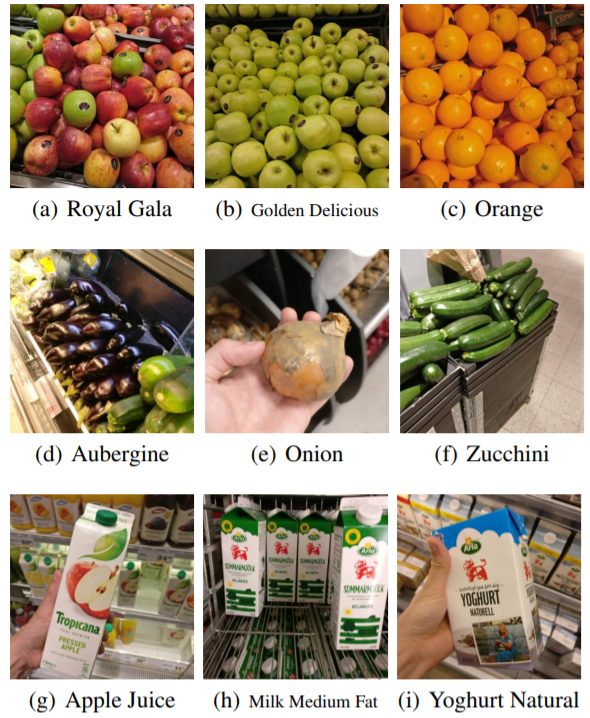
\includegraphics[scale=0.5]{PaperB/figures_and_tables/figure1.png}
		\caption{Examples of natural images in our dataset, where each image has been taken inside a grocery store. Image examples of fruits, vegetables, and refrigerated products are presented in each row respectively.}
		\label{fig:dataset_figures}
	\end{minipage}
	\hspace{10pt}
	%\vspace{-10mm}
	\begin{minipage}[b]{0.47\textwidth}
		\centering
	    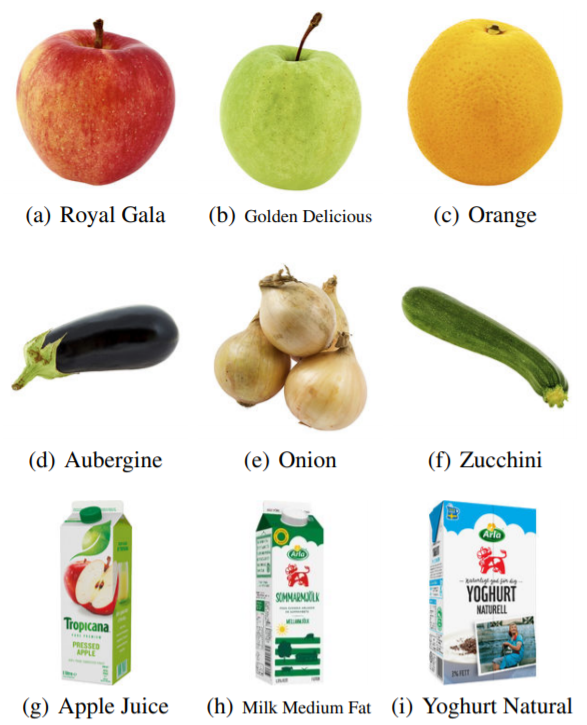
\includegraphics[scale=0.5]{PaperB/figures_and_tables/figure2.png}
		\caption{Examples of iconic images downloaded from a grocery shopping website, which corresponds to the target items in the images in Figure \ref{fig:dataset_figures}. \newline}
		\label{fig:iconic_image_figures}
	\end{minipage} 
	\vspace{-2mm}
\end{figure}



\begin{comment}

\begin{figure}
    \centering
    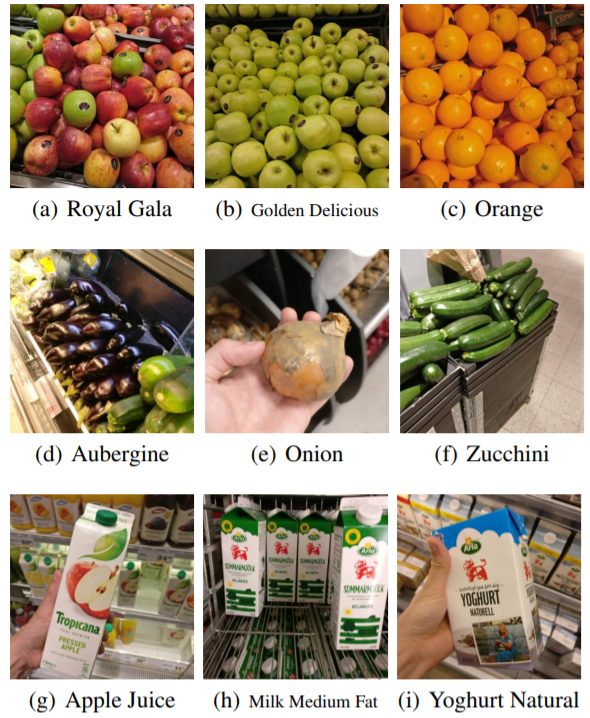
\includegraphics[scale=0.5]{PaperB/figures_and_tables/figure1.png}
    \caption{Examples of natural images in our dataset, where each image has been taken inside a grocery store. Image examples of fruits, vegetables, and refrigerated products are presented in each row respectively.}
    \label{fig:dataset_figures}
\end{figure}

\begin{figure}
    \centering
    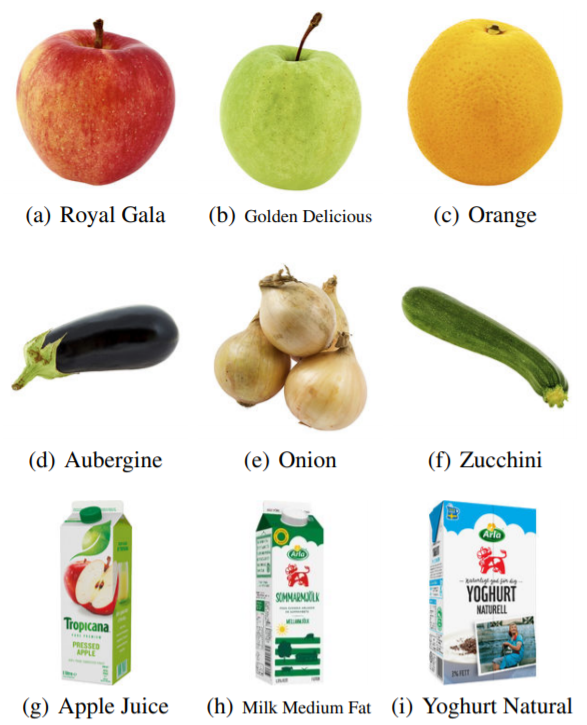
\includegraphics[scale=0.5]{PaperB/figures_and_tables/figure2.png}
    \caption{Examples of iconic images downloaded from a grocery shopping website, which corresponds to the target items in the images in Figure \ref{fig:dataset_figures}.}
    \label{fig:iconic_image_figures}
\end{figure}.
\end{comment}



For an image classification model to be capable of recognizing grocery items in the setting of grocery shopping, we need image data from grocery store environments. 
In our previous work~\citeB{B:klasson2019hierarchical}, we addressed this by collecting a novel dataset containing natural images of various raw grocery items and refrigerated products, where all images have been taken with a smartphone camera inside grocery stores to simulate a realistic shopping scenario.
In addition to the natural images, we also looked upon alternative types of grocery item data that could facilitate the classification task.
Grocery store chains commonly maintain websites where they store information about the grocery items they sell and are currently available in the store for online grocery shopping. 
For every item, there is usually an iconic image of the item with white background, a text description about the item, and also information about nutrition values, origin country, etc.
We downloaded such information from an online grocery shopping website to complement the natural images in the dataset.

To utilize the available information from the dataset for grocery item classification, we use a multi-view generative model Variational Canonical Correlation Analysis (VCCA)~\citeB{B:wang2016deep} that learns a shared representation of the natural images and the downloaded information. A view can be defined as any signal or data measured by some appropriate sensor and combining information from multiple views has previously been shown to be helpful for various image classification tasks~\citeB{B:donahue2015long-term, B:frome2013DeVISE, B:karpathy2015deep, B:kulkarni2013babytalk, B:lu2018neural, B:lu2016hierarchical, B:parikh2011relative, B:srivastava2014multimodal}. However, naively adding more additional information may not lead to improved results and even harm the performance of the model~\citeB{B:guler2014whats,B:ngiam2011multimodal}. We, therefore, perform an ablation study over the available views in the dataset with VCCA to gain insights into how each view can affect the classification performance. Moreover, VCCA allows separating the latent space into shared and private components, where the private latent spaces should hold information about a single view. This might prove useful for reducing view-specific noise in the shared latent space, which can ease the learning process of the representations we want to use for classification. We investigate the effects each view has on the learned representations of VCCA by measuring classification performances as well as visualizing the latent space for the different model settings. The contributions of this paper are the following:

\begin{itemize}[topsep=1pt, leftmargin=*] 
    \item We present a novel dataset with natural images of grocery items as well as iconic images and text descriptions for every item class (see Section 
    %subsection The Grocery Store Dataset in Results)~\citeB{B:klasson2019hierarchical}.
    \ref{paperB:sec:grocery_store_dataset})~\citeB{B:klasson2019hierarchical}.
    The natural images are taken in grocery stores in different lighting conditions and backgrounds that can be challenging settings for a computer vision-based assistive device. The additional iconic images and text descriptions make the dataset suitable for multi-view learning by combining the natural images with the extra information to obtain better classification performance.  
    
    \item We investigate how to use information from different views for the task of grocery item classification with the deep generative model VCCA (see Section \ref{paperB:sec:methods}). %subsection Methods in Experimental Procedures).
    %\ref{sec:methods}).
    This model combines information from multiple views into a low-dimensional latent representation that can be used for classification. We also select a variant of VCCA denoted VCCA-private that separates shared and private information about each view through factorization of the latent representation (see subsection Extracting Private Information of Views with VCCA-private in Experimental Procedures). 
    %\ref{sec:extracting_private_information}). 
    Furthermore, we use a standard multi-view autoencoder model called Split Autoencoder (SplitAE)~\citeB{B:ngiam2011multimodal, B:wang2015deep} for benchmarking against VCCA and VCCA-private on classification.
    
    \item We conduct experiments with SplitAE, VCCA, and VCCA-private on the task of grocery item classification with our dataset (Results).
    %Section \ref{sec:results}).
    We perform a thorough ablation study over all views in the dataset to demonstrate how each view contributes to enhancing the classification performance and conclude that utilizing the web-scraped views yields better classification results than only using the natural images (see subsection Classification Results in Results).
    % Section \ref{sec:classification_results}). 
    To gain further insights into the results, we visualize the learned latent representations of the VCCA models and discuss how the iconic images and textual descriptions impose different structures on the latent space that are beneficial for classification (see subsection Investigation of the Learned Representations in Results).
    %Section \ref{sec:investigation_of_the_learned_representations}). 
    
\end{itemize}
This work is an extended version of Klasson \etal~\citeB{B:klasson2019hierarchical}, where we first presented this dataset. In this paper, we have added a validation set of natural images from two stores that were not present in the training and test set splits from \citeB{B:klasson2019hierarchical} to avoid overfitting effects. We also demonstrate how the text descriptions can be utilized alone and along with the iconic images in a multi-view setting, while \citeB{B:klasson2019hierarchical} only experimented with the combination of natural and iconic images to build better representations of grocery items. Finally, we decode iconic images from unseen natural images as an alternative to evaluate the usefulness of the latent representations (see subsection Decoding Iconic Images from Unseen Natural Images in Results).
%(see Section \ref{sec:decoding_iconic_images}). 
As we only evaluated the decoded iconic images qualitatively in Klasson \etal~\citeB{B:klasson2019hierarchical}, we have extended the assessment by comparing the quality of the decoded images from different VCCA models with multiple image similarity metrics. 

%% RELATED WORK
Next, we discuss image datasets, food datasets, and multi-view models related to our work:

\vspace{-3mm}
\paragraph{Image Datasets} Many image datasets used in computer vision have been collected by downloading images from the web \citeB{B:deng2009imagenet, B:everingham2010pascal, B:gebru2017finegrained, B:griffin2007caltech256, B:krishna2016visualgenome, B:Krizhevsky2009cifar100, B:Lin2014MicrosoftCoco, B:nilsback2008flowers, B:song2016deep, B:WahCUB_200_2011, B:xiao2010sundatabase, B:young2014flickr30k}. 
Some datasets~\citeB{B:deng2009imagenet, B:griffin2007caltech256, B:Krizhevsky2009cifar100, B:nilsback2008flowers, B:WahCUB_200_2011} use search words with the object category in isolation, which typically returns high-quality images where the searched object is large and centered. To collect images from more real-world scenarios, searching for combinations of object categories usually returns images of two searched categories but also numerous other categories~\citeB{B:Lin2014MicrosoftCoco, B:young2014flickr30k}. 
The simplest annotation of these images is to provide a class label for the present objects. Occasionally, the dataset can use a hierarchical labeling structure and provide a fine- and coarse-grained label to objects where it is applicable. 
The annotators can also be asked to increase the possible level of supervision for the objects by, for instance, providing bounding boxes, segmentation masks, keypoints, text captions that describe the scene, and reference images of the objects~\citeB{B:gebru2017finegrained, B:krishna2016visualgenome, B:Lin2014MicrosoftCoco, B:nilsback2008flowers, B:WahCUB_200_2011, B:young2014flickr30k}. Our dataset includes reference (iconic) images of the objects that were web-scraped from a grocery store website. We also downloaded text descriptions that describe general attributes of the grocery items, such as flavor and texture, rather than the whole visual scene. The grocery items have also been labeled hierarchically in a fine- and coarse-grained manner if there exist multiple variants of specific items. For example, fine-grained classes of apples such as \textit{Golden Delicious} or \textit{Royal Gala} belongs to the coarse-grained class \textit{apple}.

\vspace{-3mm}
\paragraph{Food Datasets} 
Recognizing grocery items in their natural environments, such as grocery stores, shelves, and kitchens, have been addressed in plenty of previous works \citeB{B:geng2018fine, B:george2014recognizing, B:hsiao2010making, B:jund2016freiburg, B:klasson2019hierarchical, B:lai2011large, B:merler2007recognizing, B:singh2014bigbird, B:waltner2015mango, B:wei2019rpc, B:winlock2010toward, B:yu2018take}. The addressed tasks range from hierarchical classification, object detection, segmentation, and 3D model generation. Most of these works collect a dataset that resembles shopping or cooking scenarios, where the datasets vary in the degree of labeling, different camera views, and the data domain difference between the training and test set. 
The training sets in GroZi-120~\citeB{B:merler2007recognizing}, Grocery Products~\citeB{B:george2014recognizing}, and CAPG-GP~\citeB{B:geng2018fine} datasets were obtained by web-scraping product images of single instances on grocery web stores, while the test sets were collected in grocery stores where there can be single and multiple instances of the same item and other different items.
The RPC~\citeB{B:wei2019rpc} and TGFS~\citeB{B:yu2018take} datasets are used for object detection and classification of grocery products, where RPC is targeted for automatic checkout systems and TGFS is for the task of recognizing items purchased from self-service vending machines.
The BigBIRD~\citeB{B:singh2014bigbird} dataset and datasets from~\citeB{B:hsiao2010making, lai2011large} contain images of grocery items from multiple camera views, segmentation masks, and depth maps for 3D reconstruction of various items. 
The Freiburg Groceries~\citeB{B:jund2016freiburg} dataset contains images taken with smartphone cameras of items inside grocery stores, while its test set consists of smartphone photos in home environments with single or multiple instances from different kinds of items. The dataset presented in~\citeB{B:waltner2015mango} also contains images taken with smartphone cameras inside grocery stores to develop a mobile application for recognizing raw food items and provide details about the item, such as nutrition values and recommendations of similar items. Other works that collected datasets of raw food items, such as fruits and vegetables, focused on the standard image classification task~\citeB{B:muresan2017fruit, B:marko2013fids30} and on detecting fruits in orchards for robotic harvesting~\citeB{B:bargoti2017deepfruitdetection, B:sa2016deepfruits}. Our dataset -- the Grocery Store dataset -- shares many similarities with the mentioned works above, for instance, that all images of groceries are taken in their natural environment, the hierarchical labeling of the classes, and the iconic product images for each item in the dataset. Additionally, we have provided a text description for each item that was web-scraped along with the iconic image. As most grocery item datasets only include packaged products, we have also collected images of different fruit and vegetable classes along with packages in our dataset. 

Other examples of food datasets are those with images of food dishes, where \citeB{B:min2019survey} provides a summary of existing benchmark food datasets. The contents of these datasets range from images of food dishes~\citeB{B:bossard2014food101, B:kawano2014automatic, B:min2019ingredient, B:rich2016towards}, cooking videos~\citeB{B:damen2018scaling}, recipes~\citeB{B:marin2019learning, B:salvador2017learning, B:yagcioglu2018recipeqa}, and also restaurant-oriented information~\citeB{B:beijbom2015menu, B:xu2015geolocalized}. One major difference between recognizing groceries and food dishes is the appearance of the object categories in the images. For instance, a fruit or vegetable is usually intact and present in the image, while ingredients that are significant for recognizing a food dish may not be visible at all depending on the recipe. However, recognizing raw food items and dishes share similarities since they can appear with many different visual features in the images compared to packaged groceries, e.g., carton boxes, cans, and bottles, where the object classes have identical shape and texture. 
Another key difference is the natural environments and scenes where the images of grocery items and food dishes have been taken. Food dish images usually show the food on a plate placed on a table and, occasionally, with cutlery and a glass next to the plate. Images taken in grocery stores can cover many instances of the same item stacked close to each other in shelves, baskets, and refrigerators, while there can be multiple different kinds of items next to each other in a kitchen environment. 
To summarize, recognizing grocery items and food dishes are both challenging tasks because examples from the same category can look very different and also appear in various realistic settings in images.

\vspace{-3mm}
\paragraph{Multi-View Learning Models} There exist lots of multi-view learning approaches for data fusion of multiple features~\citeB{B:baltruvsaitis2018multimodal, B:cremer2018importance, B:frome2013DeVISE, B:fu2016semi, B:karpathy2015deep, B:ngiam2011multimodal, B:pieropan2014audio,  B:salzmann2010factorized, B:shi2019variational, B:suzuki2016joint, B:tsai2018learning, B:vedantam2017generative, B:wang2016deep, B:wu2018multimodal, B:xian2018zero, B:xu2013survey, B:zhang2016inter, B:zhao2017multi}. A common approach is to obtain a shared latent space for all views with the assumption that each view has been generated from this shared space~\citeB{B:xu2013survey}. A popular example of this is approach is Canonical Correlation Analysis (CCA)~\citeB{B:hotelling1936relations}, which aims to project two sets of variables (views) into a lower-dimensional space so that the correlation between the projections is maximized. Similar methods propose maximizing other alignment objectives for embedding the views, such as ranking losses~\citeB{B:frome2013DeVISE, B:fu2016semi, B:karpathy2015deep, B:xian2018zero}. 
There exist nonlinear extensions of CCA, e.g., Kernel CCA~\citeB{B:akaho2006kernel} and Deep CCA~\citeB{B:andrew2013deep}, that optimize their nonlinear feature mappings based on the CCA objective. 
Deep Canonically Correlated Autoencoders (DCCAE)~\citeB{B:wang2015deep} is a Deep CCA model with an autoencoding part, which aims to maximize the canonical correlation between the extracted features as well as reconstructing the input data. 
Removing the CCA objective reduces DCCAE to a standard multi-view autoencoder, e.g., Bimodal Autoencoders and Split Autoencoders (SplitAEs)~\citeB{B:ngiam2011multimodal, B:wang2015deep}, that only aim to learn a representation that best reconstructs the input data. SplitAEs aim to reconstruct two views from a representation encoded from one of the views. This approach was empirically shown to work better than Bimodal Autoencoders in \citeB{B:ngiam2011multimodal} in situations where only a single view is present at both training and test time.

Variational CCA (VCCA)~\citeB{B:wang2016deep} can be seen as an extension of CCA to deep generative models, but can also be described as a probabilistic version of SplitAEs.
VCCA uses the amortized inference procedure from Variational Autoencoders (VAEs)~\citeB{B:kingma2013auto, B:zhang2018advances} to learn the shared latent space by maximizing a lower bound on the data log-likelihood of the views. Succeeding works have proposed new learning objectives and inference methods for enabling conditional generation of views, e.g., generating an image conditioned on some text and vice versa~\citeB{B:cremer2018importance, B:shi2019variational, B:suzuki2016joint, B:vedantam2017generative, B:wu2018multimodal}. These approaches rely on fusing the views into the shared latent space as the inference procedure, which often requires tailored training and testing paradigms when views are missing. However, adding information from multiple views may not lead to improved results and can even make the model perform worse on the targeted task~\citeB{B:guler2014whats, B:ngiam2011multimodal}. This is especially the case when views have noisy observations, which complicates learning a shared latent space that combines the commonalities between the views. To avoid disturbing the shared latent space with noise from single views, some works design models which extend the shared latent space with private latent spaces for each view that should contain the view-specific variations to make learning the shared variations easier~\citeB{B:hyvarinen2000independent, B:salzmann2010factorized, B:tsai2018learning, B:wang2016deep, B:zhang2016inter}. VCCA can be extended to extract shared and private information between different views through factorization of the latent space into shared and private parts. In this paper, we investigate if the classification performance of grocery items in natural images can be improved by extracting the view-specific variations in the additional views (iconic images and product descriptions) from the shared latent space with this variant of VCCA called VCCA-private. We will experiment with treating each data point as pairs of natural images and either iconic images or text descriptions as well as triplets of natural images, iconic images, and text descriptions.
A difference between how we apply VCCA to our dataset compared to the works above is that the iconic image and text description are the same for every natural image of a specific class.  




%
\section{Related Work}\label{paperD:sec:related_work}

%In this section, we describe works in continual learning, especially memory-based, generalization in reinforcement learning, and human learning concepts related to our method.

\paragraph{Continual Learning.} One of the main goals of CL methods is to mitigate catastrophically forgetting previous tasks when learning new tasks. Approaches for retaining knowledge of previously learned tasks can be broadly divided into regularization-based methods~\citeD{D:kirkpatrick2017overcoming, D:li2017learning, D:nguyen2017variational, D:schwarz2018progress}, dynamic architectures~\citeD{D:ebrahimi2020adversarial, D:rusu2016progressive, D:yoon2017lifelong}, and memory-based methods~\citeD{D:chaudhry2019tiny, D:hayes2020remind, D:lopez2017gradient}, where the latter is the approach we focus on in this paper. Regularization-based methods put constraints on parameters important for previous tasks to mitigate forgetting and use less salient parameters for learning new tasks. Dynamic architecture approaches increase the capacity of the network by adding more parameters as new tasks are encountered. Memory-based methods mitigate forgetting by replaying samples from old tasks that are stored in a small memory buffer. This work is based on memory-based approaches, but in contrast to the traditional CL setting, we assume that we have a large amount of storage for historical data and can therefore fill the replay memory with historical data from the storage before learning new tasks~\citeD{D:klasson2021learn}. Due to processing time constraints, we need a method for selecting which historical tasks to replay at every time step.   

\paragraph{Large and Changing Action Spaces in RL.} 
Several works focus on bringing RL closer to real-world scenarios where the action spaces are large as well as can change size over time or given certain states. \citeD{D:dulac2015deep} proposes to learn action embeddings where $k$-nearest neighbors are used for selecting valid actions which the policy can select from to enable RL in large action spaces. \citeD{D:chandak2019learning} proposes to let the agent reason about which actions to take in a lower-dimensional representation space and transforms decisions in this space into actual actions which improve generalization in large action spaces when the agent infers outcomes of actions that are similar to actions already taken. \citeD{D:jain2020generalization} takes this a step further and learns action representations that should generalize to completely new actions in a zero-shot setting. \citeD{D:boutilier2018planning, chandak2020reinforcement} present how RL can be applied to stochastic action sets, while \citeD{D:chandak2020lifelong} proposes algorithms that adapt to action spaces where the set of available actions changes over time.  
Several attempts have been made to scale up Q-learning to high-dimensional or continuous action spaces. \citeD{D:he2015deep} applies Q-learning to action spaces for natural language where the Q-function is approximated by the dot-product between state and action embeddings for measuring the relevance of performing the action. \citeD{D:van2020q} comes around the maximization over all actions by instead taking the maximization over a subset of actions sampled from a learned proposal distribution, and \citeD{D:metz2017discrete} discretizes each action dimension into bins where the maximization is performed and predicts Q-value for each dimension sequentially. 
We assume that the structure of the action space is known as the number of tasks to replay grows linearly with every seen task. Since we also assume the task-horizon is known, we know the number of available actions at the end of the episodes which allows us to use a static architecture and use masking for selecting valid actions. 

\paragraph{Generalization in RL.} 
Generalization in RL is an active research field where much focus has been put on developing proper benchmark datasets for evaluating generalization capabilities of RL agents~\citeD{cobbe2019quantifying, cobbe2020leveraging, nichol2018gotta, yu2020meta}. 
Regularization techniques from supervised learning have been used to investigate whether these can enhance generalization in RL~\citeD{D:cobbe2019quantifying, farebrother2018generalization, igl2019generalization}, and also how variations in the environments help to obtain agents that generalize better~\citeD{D:packer2018assessing, zhang2018dissection}. The survey by ~\citeD{D:kirk2021survey} focuses on zero-shot policy transfer where a policy is evaluated on environments different from it was trained on. Furthermore, access to rewards or additional training is disallowed in the test environments with the aim to enable RL in real-world scenarios~\citeD{D:yang2019single}. We evaluate our learned policies on the zero-shot policy transfer setting where the goal is to mitigate catastrophic forgetting in new CL scenarios. The rewards are accessible through accuracies calculated on validation datasets, however, fine-tuning the policy during CL training is prohibited.  


%There are also works that try to learn in large action spaces and also generalize fast to new actions [add references].  

%\MK{Mention zero-shot policy transfer and what it is.}



%\paragraph{Human Learning.} We draw inspiration from human learning techniques, especially spaced repetition~\citep{dempster1989spacing}, in our approach for learning replay scheduling policies. 

%\MK{
%Some links on human learning and ML with spaced repetition 
%\begin{itemize}
%    \item Enhancing human learning via spaced repetition optimization, Tabibian et al. \url{https://www.pnas.org/content/pnas/116/10/3988.full.pdf}, \url{http://learning.mpi-sws.org/memorize/}
%    \item Accelerating Human Learning with Deep Reinforcement Learning, Reddy et al.
%    \item Unbounded Human Learning: Optimal Scheduling for Spaced Repetition Reddy et al. \url{https://dl.acm.org/doi/abs/10.1145/2939672.2939850}
%\end{itemize}}
%
\section{Method}\label{paperC:sec:method}


In this section, we describe our new problem setting in CL where historical data are available while the processing time is limited when learning new tasks. To this end, we present our method for learning replay schedules in CL where the idea is to learn schedules of which tasks the network should replay at different times. 
%In this section, we describe our method for learning replay schedules in CL. The idea is to learn schedules of which tasks %memory examples 
%the network should replay at different times. 
We use Monte Carlo tree search (MCTS)~\citeC{C:coulom2006efficient} to learn a scheduling policy by encouraging searches for promising replay schedules based on the classification accuracy. 


\subsection{Problem Setting}\label{paperC:sec:problem_setting}

We focus on a slightly new setting, considering the needs for CL in the real-world where all historical data can be available since data storage is cheap. 
However, as this data volume is typically huge, we are often prohibited from replaying all historical data due to processing time constraints. 
Therefore, the goal is to determine which historical tasks to revisit and sample a small replay memory from the selected tasks to mitigate catastrophic forgetting as efficiently as possible. 

\setlength{\abovedisplayskip}{0pt}
\setlength{\belowdisplayskip}{0pt}
\setlength{\abovedisplayshortskip}{0pt}
\setlength{\belowdisplayshortskip}{0pt}

Here, we introduce the notation of our problem setting which resembles the traditional CL setting for image classification. We let a neural network $f_{\vtheta}$, parameterized by $\vtheta$, learn $T$ tasks sequentially from the datasets $\gD_1, \dots, \gD_T$ arriving one at a time. 
The $t$-th dataset $\gD_t = \{(\vx_{t}^{(i)}, y_{t}^{(i)})\}_{i=1}^{N_{t}}$ consists of $N_t$ samples where $\vx_{t}^{(i)}$ and $y_{t}^{(i)}$ are the $i$-th data point and class label respectively. The training objective at task $t$ is given by 
\begin{align}
	\underset{\vtheta}{\text{min}} \sum_{i=1}^{N_t} \ell(f_{\vtheta}(\vx_t^{(i)}), y_{t}^{(i)}),
\end{align}
where $\ell(\cdot)$ is the loss function, e.g., cross-entropy loss in our case. 
When learning task $t$, the network $f_{\vtheta}$ is at risk of catastrophically forgetting the previous $t-1$ tasks. Next, we describe our method for constructing this replay memory.  

We assume that historical data from old tasks are accessible at any time step $t$. 
However, due to processing time constraints, we can only fill a small replay memory $\gM$ with $M$ historical samples for replay. 
The challenge then becomes how to select the $M$ replay samples to efficiently retain knowledge of old tasks. We focus on selecting the samples on task-level by deciding on the task proportion $(p_1, \dots, p_{t-1})$ of samples to fetch from each task, where $p_{i} \geq 0$ is the proportion of $M$ samples from task $i$ to place in $\gM$ and $\sum_{i=1}^{t-1} p_i = 1$. To simplify the selection of which tasks to replay, we construct a discrete set of possible task proportions that can be used for constructing $\gM$.



 %%% RS-MCTS EXAMPLE FIGURE 
\begin{figure*}[t]
\centering 
\setlength{\figwidth}{.77\textwidth}
\setlength{\figheight}{.3\textheight}
\definecolor{color0}{rgb}{0.945098039215686,0.435294117647059,0.125490196078431}
\definecolor{color1}{rgb}{0.843137254901961,0.6,0.133333333333333}
\definecolor{color2}{rgb}{0.250980392156863,0.337254901960784,0.631372549019608}
\definecolor{color3}{rgb}{1,0.498039215686275,0}
\definecolor{color4}{rgb}{0.94509803921,0.23529411764,0.12549019607}
\definecolor{color5}{rgb}{0.94509803921,0.23529411764,0.12549019607}

\resizebox{0.95\textwidth}{!}{
\begin{tikzpicture}[
    roundnode/.style={circle, draw=color3, text=color3, very thick, minimum size=7mm},
    squarednode/.style={rectangle, draw=black, fill=white, text=black, very thick, minimum size=7mm, align=center, rounded corners},
    %tasknode/.style={rectangle, draw=blue!50, fill=blue!10, text=black, very thick, minimum size=7mm, align=center, depth=2cm, rounded corners},
    %task/.style={rectangle, rounded corners, thick,inner sep=3pt},
    ]
    %%% Task 1 level
    \draw[draw=blue!50, fill=blue!10, very thick, rounded corners] (0,0) rectangle (16,-2);
    \node[squarednode] (dataset1) at (1.,-1) { \textbf{Task 1} \\ 
\includegraphics[width=0.08\textwidth]{PaperC/figures/mcts_tikz/dataset_two_images/dataset1.eps}};
    \node[squarednode] (v1) at (9,-1) {\large $\emptyset$};
    
    %%% Task 2 level
    \draw[draw=red!50, fill=red!10, very thick, rounded corners] (0,-2) rectangle (16,-4);
    
    \node[squarednode] (dataset2) at (1.,-3) { \textbf{Task 2} \\ 
\includegraphics[width=0.08\textwidth]{PaperC/figures/mcts_tikz/dataset_two_images/dataset2.eps}};
    \node[squarednode, text=color3] (v2) at (9,-3) {
\includegraphics[width=0.045\textwidth]{PaperC/figures/mcts_tikz/vertical_rs/task1_only.eps}};
    \draw[<-] (v2) -- (v1);
    
    %%% Task 3 level
    \draw[draw=color3!50, fill=color3!10, very thick, rounded corners] (0,-4) rectangle (16,-6);
    \node[squarednode] (dataset3) at (1.,-5) { \textbf{Task 3} \\ 
\includegraphics[width=0.08\textwidth]{PaperC/figures/mcts_tikz/dataset_two_images/dataset3.eps}};
    \node[squarednode, text=color3] (v3_beg) at (5,-5) {
\includegraphics[width=0.045\textwidth]{PaperC/figures/mcts_tikz/vertical_rs/task1_only.eps}};
    \draw[<-, blue, very thick] (v3_beg) -- (v2);
    
    \node[squarednode, text=color3] (v3_mid) at (9,-5) {
\includegraphics[width=0.045\textwidth]{PaperC/figures/mcts_tikz/vertical_rs/equal_task3.eps}};
    \draw[<-, red, very thick] (v3_mid) -- (v2);
    
    \node[squarednode, text=color3] (v3_end) at (13,-5) {
\includegraphics[width=0.045\textwidth]{PaperC/figures/mcts_tikz/vertical_rs/task2_only.eps}};
    \draw[<-, purple, very thick] (v3_end) -- (v2);
    
    %%% Task 4 level
    \draw[draw=magenta!50, fill=magenta!10, very thick, rounded corners] (0,-6) rectangle (16,-8);
    
    \node[squarednode] (dataset4) at (1.,-7) { \textbf{Task 4} \\ 
\includegraphics[width=0.08\textwidth]{PaperC/figures/mcts_tikz/dataset_two_images/dataset4.eps}};
    
    \node[squarednode, text=color3] (v41_beg) at (4,-7) {
\includegraphics[width=0.045\textwidth]{PaperC/figures/mcts_tikz/vertical_rs/task1_only.eps}};
    \draw[<-, blue, very thick] (v41_beg) -- (v3_beg);
    %\draw[<-] (v4_beg) -- (v3_mid);
    %\draw[<-] (v4_beg) -- (v3_end);
    
    \node[] (v41_dots) at (5,-7) {\large $\cdots$};
    %\draw[<-] (v4_dots1) -- (v3_beg);%\draw[<-, dashed] (v4_dots1) -- (v3_beg);
    %\draw[<-] (v4_dots1) -- (v3_mid);
    %\draw[<-] (v4_dots1) -- (v3_end);
    
    \node[squarednode, text=color3] (v41_end) at (6,-7) {
\includegraphics[width=0.045\textwidth]{PaperC/figures/mcts_tikz/vertical_rs/task3_only.eps}};
    \draw[<-] (v41_end) -- (v3_beg);
    
    \node[squarednode, text=color3] (v42_beg) at (7.1,-7) {
\includegraphics[width=0.045\textwidth]{PaperC/figures/mcts_tikz/vertical_rs/task1_only.eps}};
    \draw[<-] (v42_beg) -- (v3_mid);
    
    \node[] (v42_dots1) at (8,-7) {\large $\cdots$};
    
    \node[squarednode, text=color3] (v42_mid) at (9,-7) {
\includegraphics[width=0.045\textwidth]{PaperC/figures/mcts_tikz/vertical_rs/equal_task4.eps}};
    \draw[<-, red, very thick] (v42_mid) -- (v3_mid);
    
    \node[] (v42_dots2) at (10,-7) {\large $\cdots$};
    
    \node[squarednode, text=color3] (v42_end) at (11,-7) {
\includegraphics[width=0.045\textwidth]{PaperC/figures/mcts_tikz/vertical_rs/task3_only.eps}};
    \draw[<-] (v42_end) -- (v3_mid);
    %\node[squarednode, text=color3] (v4_end1) at (6.5,-7) {
\includegraphics[width=0.08\textwidth]{PaperC/figures/mcts_tikz/replay_batches/task3_only.eps}};
    %\draw[<-] (v4_end1) -- (v3_beg);
    
    \node[squarednode, text=color3] (v43_beg) at (12.1,-7) {
\includegraphics[width=0.045\textwidth]{PaperC/figures/mcts_tikz/vertical_rs/task1_only.eps}};
    \draw[<-] (v43_beg) -- (v3_end);
    
    \node[] (v43_dots) at (13,-7) {\large $\cdots$};
    %\draw[<-] (v4_dots2) -- (v3_beg);
    %\draw[<-] (v4_dots2) -- (v3_mid);
    %\draw[<-] (v4_dots2) -- (v3_end);
    
    \node[squarednode, text=color3] (v43_end) at (14,-7) {
\includegraphics[width=0.045\textwidth]{PaperC/figures/mcts_tikz/vertical_rs/task3_only.eps}};
    \draw[<-, purple, very thick] (v43_end) -- (v3_end);
    %\draw[<-] (v4_end) -- (v3_mid);
    %\draw[<-, purple, very thick] (v4_end) -- (v3_end);


    %%% Task 5 level
    \draw[draw=green!50, fill=green!10, very thick, rounded corners] (0,-8) rectangle (16,-10);
    \node[squarednode] (dataset5) at (1.,-9) { \textbf{Task 5} \\ 
\includegraphics[width=0.08\textwidth]{PaperC/figures/mcts_tikz/dataset_two_images/dataset5.eps}};
    
    \node[squarednode, text=color3] (v51_beg) at (3,-9) {
\includegraphics[width=0.045\textwidth]{PaperC/figures/mcts_tikz/vertical_rs/task1_only.eps}};
    \draw[<-, blue, very thick] (v51_beg) -- (v41_beg);
    %\draw[<-] (v5_beg) -- (v4_dots1);
    %\draw[<-] (v5_beg) -- (v4_mid);
    %\draw[<-] (v5_beg) -- (v4_dots2);
    %\draw[<-] (v5_beg) -- (v4_end);
    
    \node[] (v51_dots) at (4,-9) {\large $\cdots$};
    %\draw[<-] (v5_dots1) -- (v4_beg1);
    %\draw[<-] (v5_dots1) -- (v4_dots1);
    %\draw[<-] (v5_dots1) -- (v4_mid);
    %\draw[<-] (v5_dots1) -- (v4_dots2);
    %\draw[<-] (v5_dots1) -- (v4_end);
    
    \node[squarednode, text=color3] (v51_end) at (5,-9) {
\includegraphics[width=0.045\textwidth]{PaperC/figures/mcts_tikz/vertical_rs/task4_only.eps}};
    \draw[<-] (v51_end) -- (v41_beg);
    
    %\node[squarednode, text=color3] (v52_beg) at (5,-9) {
\includegraphics[width=0.045\textwidth]{PaperC/figures/mcts_tikz/vertical_rs/task1_only.eps}};
    
    %\node[squarednode, text=color3] (v5_mid_low) at (6,-9) {\includegraphics[width=0.06\textwidth]{PaperC/figures/mcts_tikz/replay_batches/task5_middle0.eps}};
    %\draw[<-] (v5_mid_low) -- (v4_beg);
    %\draw[<-] (v5_mid_low) -- (v4_dots1);
    %\draw[<-] (v5_mid_low) -- (v4_mid);
    %\draw[<-] (v5_mid_low) -- (v4_dots2);
    %\draw[<-] (v5_mid_low) -- (v4_end);
    
    \node[] (v52_dots) at (6,-9) {\large $\cdots$};
    \draw[<-, dashed] (v52_dots) -- (v41_end);
    
    \node[] (v53_dots) at (7.1,-9) {\large $\cdots$};
    \draw[<-, dashed] (v53_dots) -- (v42_beg);
    
     \node[] (v54_dots) at (8,-9) {\large $\cdots$};
    %\draw[<-] (v5_dots2) -- (v4_beg);
    %\draw[<-] (v5_dots2) -- (v4_dots1);
    %\draw[<-] (v5_dots2) -- (v4_mid);
    %\draw[<-] (v5_dots2) -- (v4_dots2);
    %\draw[<-] (v5_dots2) -- (v4_end);
    
    \node[squarednode, text=color3] (v52_mid) at (9,-9) {
\includegraphics[width=0.045\textwidth]{PaperC/figures/mcts_tikz/vertical_rs/equal_task5.eps}};
    \draw[<-, red, very thick] (v52_mid) -- (v42_mid);
    %\draw[<-] (v5_mid) -- (v4_beg);
    %\draw[<-] (v5_mid) -- (v4_dots1);
    %\draw[<-, red, very thick] (v5_mid) -- (v4_mid);
    %\draw[<-] (v5_mid) -- (v4_dots2);
    %\draw[<-] (v5_mid) -- (v4_end);
    
    \node[] (v55_dots) at (10,-9) {\large $\cdots$};
    
    \node[] (v56_dots) at (11,-9) {\large $\cdots$};
    \draw[<-, dashed] (v56_dots) -- (v42_end);
    
    \node[] (v57_dots) at (12.1,-9) {\large $\cdots$};
    \draw[<-, dashed] (v57_dots) -- (v43_beg);
    %\draw[<-] (v5_dots3) -- (v4_beg);
    %\draw[<-] (v5_dots3) -- (v4_dots1);
    %\draw[<-] (v5_dots3) -- (v4_mid);
    %\draw[<-] (v5_dots3) -- (v4_dots2);
    %\draw[<-] (v5_dots3) -- (v4_end);
    
    %\node[squarednode, text=color3] (v5_mid_high) at (12,-9) {\includegraphics[width=0.06\textwidth]{PaperC/figures/mcts_tikz/replay_batches/task5_middle1.eps}};
    %\draw[<-] (v5_mid_high) -- (v4_beg);
    %\draw[<-] (v5_mid_high) -- (v4_dots1);
    %\draw[<-] (v5_mid_high) -- (v4_mid);
    %\draw[<-] (v5_mid_high) -- (v4_dots2);
    %\draw[<-] (v5_mid_high) -- (v4_end);
    
    \node[squarednode, text=color3] (v53_beg) at (13,-9) {
\includegraphics[width=0.045\textwidth]{PaperC/figures/mcts_tikz/vertical_rs/task1_only.eps}};
    \draw[<-] (v53_beg) -- (v43_end);
    
    \node[black] (v58_dots) at (14,-9) {\large $\cdots$};
    
    %\draw[--, dashed] (v5_dots4) -- (v43_dots);
    %\draw[<-] (v5_dots4) -- (v4_mid);
    %\draw[<-] (v5_dots4) -- (v4_dots2);
    %\draw[<-] (v5_dots4) -- (v4_end);
    
    \node[squarednode, text=color3] (v53_end) at (15,-9) {
\includegraphics[width=0.045\textwidth]{PaperC/figures/mcts_tikz/vertical_rs/task4_only.eps}};
    \draw[<-, purple, very thick] (v53_end) -- (v43_end);
    %\draw[<-] (v5_end) -- (v4_beg);
    %\draw[<-] (v5_end) -- (v4_dots1);
    %\draw[<-] (v5_end) -- (v4_mid);
    %\draw[<-] (v5_end) -- (v4_dots2);
    %\draw[<-, purple, very thick] (v5_end) -- (v4_end);
\end{tikzpicture}
}
  % \tikzexternalenable
  % \vspace{-15pt}
  % \includegraphics[width=0.95\linewidth]{pixeldag.png}
  % \vspace{-15pt}

\vspace{-2mm}
\caption{An exemplar tree of replay memory compositions from the proposed discretization method described in Section \ref{sec:replay_scheduling_in_continual_learning} for Split MNIST. The replay memories from one replay schedule are found by traversing from task 1-5 through the tree on the right hand side. The replay memory compositions have been structured according to the task where they can be used for replay. Note that the replay memory at task 1 is the empty set, i.e., $\gM = \emptyset$. Example images for each task are shown on the left.
}
\vspace{-3mm}
\label{fig:replay_scheduling_mcts_tree_example}
\end{figure*}



\subsection{Replay Scheduling in Continual Learning}\label{sec:replay_scheduling_in_continual_learning}

In this section, 
we describe our replay scheduling method for selecting the replay memory at different time steps. We define a replay schedule as a sequence $S = (\va_1, \dots, \va_{T-1})$, where $\va_i = (a_1, \dots, a_{T-1})$ for $1 \leq i \leq T-1$ is the sequence of task proportions used for determining how many samples per task to fill the replay memory with at task $i$. To make the selection of task proportions tractable, we construct an action space with a discrete number of choices for %the 
task proportions from old tasks. 
We use the following method to construct this action space: At the time to learn task $t$, we have $t-1$ historical tasks that we can choose from. We create $t-1$ bins $\vb_t = [b_1, \dots, b_{t-1}]$ and choose a task index to sample for each bin $b_i \in \{1, \dots, t-1 \}$. We treat the bins as interchangeable and only keep the unique choices. 
For example, at task 3, we have seen task 1 and 2, so the unique choices of vectors are $[1,1], [1,2], [2,2]$, where $[1,1]$ indicates that all memory samples are from task 1, $[1,2]$ indicates that half memory is from task 1 and the other half are from task etc. The task proportions are then computed by counting the number of occurrences of each task index in $\vb_t$ and dividing by $t-1$, such that $\va_t = \texttt{bincount}(\vb_t) / (t-1)$. 
If the memory size $M$ is not divisible by the task proportion value for task $i$, we round the number of replay samples from task $i$, i.e., $a_i \cdot M$, up or down accordingly while keeping the memory size fixed.
From this specification, we can build a tree of different replay schedules to evaluate with the network.


Figure \ref{fig:replay_scheduling_mcts_tree_example} shows an example of a replay schedule tree with Split MNIST~\citep{zenke2017continual} 
where the memory size is $M=8$. %where the memory size has been set to $M=8$. 
The figure shows the current tasks with example images of the task classes on the left, and the right side shows examples of possible replay memories that can be evaluated. The memory starts as the empty set, i.e. $\gM_1 = \emptyset$, at task 1. Before learning task 2, $\gM_2$ is filled with $M$ task 1 examples since this is the only task seen so far. At task 3, the memory compositions we can choose from are $M$ examples from either task 1 or 2, as well as equally filling $\gM_3$ with four examples each from both tasks. 
A replay schedule is represented as a path traversal of different replay memory compositions from task 1 to task 5. We have color-coded three examples of possible schedules in Figure \ref{fig:replay_scheduling_mcts_tree_example} to use for illustration: the \textcolor{blue}{blue} path represents a replay schedule where only task 1 examples are replayed. %at all future tasks. 
The \textcolor{red}{red} path represents using an equally distributed amount of memory samples per task in the memory, and the \textcolor{purple}{purple} path represents a schedule where the memory is filled $M$ examples from the previously visited task. Note that all other possible paths in the tree are also valid replay schedules. 






\subsection{Monte Carlo Tree Search for Replay Schedules}
\label{paperC:sec:mcts_for_replay_scheduling}

In this section, we describe how we enable using MCTS for studying the benefits of replay scheduling in CL scenarios.
The tree-shaped action space of task proportions described in Section \ref{paperC:sec:replay_scheduling_in_continual_learning} grows fast with the number of tasks, which complicates studying replay scheduling in datasets with longer task-horizons. Since the search space is too big for using exhaustive searches, 
we need a scalable method that enables tree searches in large action spaces.
To this end, we propose to use MCTS since it has been successful in applications with large action spaces~\citeC{C:browne2012survey, C:chaudhry2018feature, C:gelly2006modification, C:silver2016mastering}. In our case, MCTS concentrates the search for replay schedules in directions with promising CL performance in the environment. We use MCTS in an ideal CL setting, wherein multiple episodes are allowed, for demonstration purposes to show that replay scheduling can be critical for the CL performance. 

Each memory composition in the action space corresponds to a node that can be visited by MCTS. For example, in Figure \ref{fig:replay_scheduling_mcts_tree_example}, the nodes correspond to the possible memory examples which can be visited during the MCTS rollouts.
At task $t$, the node $v_t$ is related to a task proportions $\va_{t}$ used for retrieving a replay memory from the historical data. 
We store the related task proportion $\va_t$ from every visited node $v_t$ in the replay schedule $S$. 
The final replay schedule is then used for constructing the replay memories at each task during the CL training.  
Next, we briefly outline the MCTS steps for performing the replay schedule search (more details in Appendix \ref{app:rs_mcts_algorithm}):

\vspace{-1mm}
\begin{itemize}[leftmargin=*, topsep=0pt, noitemsep, label={}]
	\item {\bf Selection.} During a rollout, the current node $v_t$ either moves randomly to unvisited children, or selects the next node by evaluating the Upper Confidence Tree (UCT)~\citeC{C:kocsis2006bandit} if all children has been visited earlier.
	The child $v_{t+1}$ with the highest UCT score is selected using the function from \cite{chaudhry2018feature}:
	\begin{align}\label{eq:uct}
		UCT(v_t, v_{t+1}) = \text{max}(q(v_{t+1})) + C \sqrt{\frac{2 \log(n(v_{t}))}{n(v_{t+1})}},
	\end{align}
	where $q(\cdot)$ is the reward function, $C$ the exploration constant, and $n(\cdot)$ the number of node visits. 
	
	\item {\bf Expansion.} Whenever the current node $v_t$ has unvisited child nodes, the search tree is expanded with one of the unvisited child nodes $v_{t+1}$ selected with uniform sampling. 
	
	\item {\bf Simulation and Reward.} After expansion, the succeeding nodes are selected randomly until reaching a terminal node $v_T$. The task proportions from the visited nodes in the rollout constitutes the replay schedule $S$. After training the network using $S$ for replay, we calculate the reward for the rollout is given by $r = \frac{1}{T} \sum_{i=1}^T A_{T, i}^{(val)}$, where $A_{T, i}^{(val)}$ is the validation accuracy of task $i$ at task $T$.  
	
	\item {\bf Backpropagation.} Reward $r$ is backpropagated from the expanded node $v_t$ to the root $v_1$, where the reward function $q(\cdot)$ and number of visits $n(\cdot)$ are updated at each node. 
\end{itemize}










%
\section{Experiments}\label{paperD:sec:experiments}


We evaluate our RL-based framework using DQN~\citeD{D:mnih2013playing, D:mnih2015human} and A2C~\citeD{D:mnih2016asynchronous} for learning policies that generalize to new CL scenarios. We show that the learned policies can efficiently mitigate catastrophic forgetting in CL environments with new task orders and datasets that are unseen during training. Full details on experimental settings and additional results are in Appendix \ref{paperD:app:experimental_settings} and \ref{paperD:app:additional_experimental_results}. Code will be made publicly available upon acceptance. 


\vspace{-3mm}
\paragraph{Datasets and Network Architectures.} We conduct experiments on four CL benchmark datasets: Split MNIST~\citeD{D:lecun1998gradient, D:zenke2017continual}, FashionMNIST~\citeD{D:xiao2017fashion}, Split notMNIST~\citeD{D:bulatov2011notMNIST}, Permuted MNIST~\citeD{D:goodfellow2013empirical}, and Split CIFAR-10~\citeD{D:krizhevsky2009learning}. We randomly sample 15\% of training data for each task to use for validation, and keep the original test sets intact. 
We use multi-head output layers for all datasets and assume task labels are available at test time~\citeD{D:van2019three}. A 2-layer MLP with 256 hidden units for Split MNIST, Split FashionMNIST, and Split notMNIST. For Split CIFAR-10, we the same ConvNet architecture used in \citeD{D:adel2019continual, D:schwarz2018progress, D:vinyals2016matching}.

\vspace{-3mm}
\paragraph{Generating CL Environments.} We generate multiple CL environments with pre-set random seeds for initializing the network parameters $\vphi$ and shuffling the task order. See Appendix \ref{paperD:app:experimental_settings} for details on the pre-set seeds. 
%The pre-set random seeds are in the range $0-49$, such that we have 50 environments for each dataset. 
We shuffle the task order by permuting the class order and then split the classes into 5 pairs (tasks) with 2 classes/pair. 
%For environments with seed $0$, we keep the original task order in the dataset. 
Taking a step at task $t$ in the CL environments involves training the CL network on the $t$-th dataset with a replay memory $\gM_t$ from the discrete action space described in Appendix \ref{paperD:app:action_space}. 
To speed up the experiments with the RL algorithms, we run a breadth-first search (BFS) through the discrete action space and save the classification results for re-use during policy learning. Note that the action space has 1050 possible paths of replay schedules for the 5-task datasets, which makes the environment generation time-consuming. More specifically, generating a CL environment for one seed with Split MNIST took on around 9.5 hours on average on a NVIDIA GeForce RTW 2080Ti.   
Hence, we only generate environments where the replay memory size $M=10$ have been used, and leave analysis of different memory sizes as future work. 
%The CL environments that we used will be provided in the public code. 

\begin{figure}[t]
	\centering
	\setlength{\figwidth}{0.26\textwidth}
	\setlength{\figheight}{.14\textheight}
	\begin{subfigure}[t]{0.48\textwidth}
		\centering
		



\pgfplotsset{every axis title/.append style={at={(0.5,0.85)}}}
\pgfplotsset{every tick label/.append style={font=\tiny}}
\pgfplotsset{every major tick/.append style={major tick length=2pt}}
\pgfplotsset{every minor tick/.append style={minor tick length=1pt}}
\pgfplotsset{every axis x label/.append style={at={(0.5,-0.22)}}}
\pgfplotsset{every axis y label/.append style={at={(-0.30,0.5)}}}
\begin{tikzpicture}
\tikzstyle{every node}=[font=\scriptsize]
\definecolor{color0}{rgb}{0.12156862745098,0.466666666666667,0.705882352941177}
\definecolor{color1}{rgb}{1,0.498039215686275,0.0549019607843137}
\definecolor{color2}{rgb}{0.172549019607843,0.627450980392157,0.172549019607843}
\definecolor{color3}{rgb}{0.83921568627451,0.152941176470588,0.156862745098039}
\definecolor{color4}{rgb}{0.580392156862745,0.403921568627451,0.741176470588235}
\definecolor{color5}{rgb}{0.549019607843137,0.337254901960784,0.294117647058824}
\definecolor{color6}{rgb}{0.890196078431372,0.466666666666667,0.76078431372549}

\begin{groupplot}[group style={group size= 2 by 1, horizontal sep=1.00cm, vertical sep=1.20cm}]

\nextgroupplot[title=Seed 11,
height=\figheight,
legend cell align={left},
legend columns=-1, 
legend style={
	nodes={scale=0.85},
	fill opacity=0.8,
	draw opacity=1,
	text opacity=1,
    at={(-0.13,1.36)},%at={(0.10,1.29)},
    anchor=south west,
    draw=white!80!black
},
minor xtick={25, 75},
minor ytick={},
tick align=outside,
tick pos=left,
%title={Labels: [[7, 8], [2, 6], [4, 5], [1, 3], [0, 9]]},
width=\figwidth,
x grid style={white!69.0196078431373!black},
xlabel={Eval. Steps},
xminorgrids,
xmajorgrids,
xmin=-3.95, xmax=104.95,
xtick style={color=black},
xtick={-25,0,50,100,125},
xticklabels={-25,0,50,100,125},
y grid style={white!69.0196078431373!black},
%ylabel={ACC},
ymajorgrids,
ymin=0.908595944220984, ymax=0.972076868974256,
ytick style={color=black},
ytick={0.9,0.91,0.92,0.93,0.94,0.95,0.96,0.97,0.98},
yticklabels={90,91,92,93,94,95,96,97,98}
]
\addplot [semithick, color0]
table {%
	1 0.949812457561493
	2 0.949775466918945
	3 0.960892503261566
	4 0.956866431236267
	5 0.945231194496155
	6 0.945613367557526
	7 0.94686802148819
	8 0.952512142658234
	9 0.943398241996765
	10 0.944289662837982
	11 0.930401303768158
	12 0.950187075138092
	13 0.946467769145966
	14 0.943979327678681
	15 0.942831747531891
	16 0.943993356227875
	17 0.944837226867676
	18 0.941551671028137
	19 0.931446702480316
	20 0.949583513736725
	21 0.953074641227722
	22 0.952990527153015
	23 0.939547181129456
	24 0.942692797183991
	25 0.956659049987793
	26 0.954558956623077
	27 0.956728446483612
	28 0.952419261932373
	29 0.953414702415466
	30 0.949406821727753
	31 0.96032018661499
	32 0.938822565078735
	33 0.941302559375763
	34 0.945325396060944
	35 0.949670062065124
	36 0.940685608386993
	37 0.946110789775848
	38 0.936599233150482
	39 0.952321965694427
	40 0.948934230804443
	41 0.942440538406372
	42 0.938124449253082
	43 0.949964995384216
	44 0.942903997898102
	45 0.954234335422516
	46 0.95132431268692
	47 0.948090310096741
	48 0.938373746871948
	49 0.942048320770264
	50 0.950774230957031
	51 0.948220450878143
	52 0.944915144443512
	53 0.934470863342285
	54 0.946825733184814
	55 0.947917900085449
	56 0.931744492053986
	57 0.948268630504608
	58 0.940266535282135
	59 0.949667906761169
	60 0.941861910820007
	61 0.946911418437958
	62 0.949336833953857
	63 0.93532523393631
	64 0.944827678203583
	65 0.944855451583862
	66 0.943393461704254
	67 0.941029033660889
	68 0.939231975078583
	69 0.938024179935455
	70 0.940667865276337
	71 0.933951034545898
	72 0.942696425914764
	73 0.946916031837463
	74 0.937888109683991
	75 0.940196809768677
	76 0.936573145389557
	77 0.932672383785248
	78 0.942083840370178
	79 0.936137390136719
	80 0.941790580749512
	81 0.941255300045013
	82 0.937389364242554
	83 0.903695275783539
	84 0.940915014743805
	85 0.938173484802246
	86 0.934200079441071
	87 0.943309750556946
	88 0.940444509983063
	89 0.93537590265274
	90 0.931826453208923
	91 0.936913092136383
	92 0.938212811946869
	93 0.946724779605866
	94 0.928359398841858
	95 0.941560471057892
	96 0.930597925186157
	97 0.93455456495285
	98 0.934019336700439
	99 0.928332870006561
	100 0.940782828330994
};
\addlegendentry{DQN}
\addplot [semithick, color1]
table {%
	1 0.930601587295532
	2 0.966550159454346
	3 0.966550159454346
	4 0.966192562580109
	5 0.969191372394562
	6 0.96504182100296
	7 0.948443615436554
	8 0.948443615436554
	9 0.948443615436554
	10 0.948443615436554
	11 0.961694481372833
	12 0.958381764888763
	13 0.965007197856903
	14 0.965007197856903
	15 0.961694481372833
	16 0.965007197856903
	17 0.961694481372833
	18 0.958381764888763
	19 0.961694481372833
	20 0.965007197856903
	21 0.958381764888763
	22 0.958381764888763
	23 0.955069048404694
	24 0.958381764888763
	25 0.965007197856903
	26 0.958381764888763
	27 0.958381764888763
	28 0.961694481372833
	29 0.961694481372833
	30 0.955069048404694
	31 0.965007197856903
	32 0.958381764888763
	33 0.958381764888763
	34 0.958381764888763
	35 0.955069048404694
	36 0.958381764888763
	37 0.955069048404694
	38 0.955069048404694
	39 0.951756331920624
	40 0.955069048404694
	41 0.948443615436554
	42 0.955069048404694
	43 0.955069048404694
	44 0.955069048404694
	45 0.948443615436554
	46 0.951756331920624
	47 0.948443615436554
	48 0.955069048404694
	49 0.958381764888763
	50 0.951756331920624
	51 0.951756331920624
	52 0.958381764888763
	53 0.951756331920624
	54 0.958381764888763
	55 0.955069048404694
	56 0.951756331920624
	57 0.958381764888763
	58 0.955069048404694
	59 0.958381764888763
	60 0.958381764888763
	61 0.961694481372833
	62 0.958381764888763
	63 0.958381764888763
	64 0.958381764888763
	65 0.958381764888763
	66 0.961694481372833
	67 0.961694481372833
	68 0.951756331920624
	69 0.958381764888763
	70 0.961694481372833
	71 0.961694481372833
	72 0.958381764888763
	73 0.961694481372833
	74 0.961694481372833
	75 0.960777387619019
	76 0.961694481372833
	77 0.961694481372833
	78 0.958381764888763
	79 0.961694481372833
	80 0.961694481372833
	81 0.961694481372833
	82 0.960777387619019
	83 0.965007197856903
	84 0.965007197856903
	85 0.964090104103088
	86 0.958381764888763
	87 0.964090104103088
	88 0.964090104103088
	89 0.962255916595459
	90 0.965007197856903
	91 0.961694481372833
	92 0.964090104103088
	93 0.964090104103088
	94 0.965007197856903
	95 0.963173010349274
	96 0.964090104103088
	97 0.963173010349274
	98 0.964090104103088
	99 0.959860293865204
	100 0.964090104103088
};
\addlegendentry{A2C}
\addplot [semithick, color2]
table {%
	1 0.941761815547943
	2 0.941761815547943
	3 0.941761815547943
	4 0.943232760429382
	5 0.943232760429382
	6 0.956506490707397
	7 0.957273149490356
	8 0.958714089393616
	9 0.958714089393616
	10 0.956937248706818
	11 0.95984382390976
	12 0.958714089393616
	13 0.958714089393616
	14 0.958714089393616
	15 0.958714089393616
	16 0.960152294635773
	17 0.95927184343338
	18 0.95927184343338
	19 0.954713544845581
	20 0.956052875518799
	21 0.9589133477211
	22 0.9589133477211
	23 0.9589133477211
	24 0.9589133477211
	25 0.9589133477211
	26 0.9589133477211
	27 0.9589133477211
	28 0.958693928718567
	29 0.956346516609192
	30 0.9589133477211
	31 0.9589133477211
	32 0.9589133477211
	33 0.9589133477211
	34 0.9589133477211
	35 0.9589133477211
	36 0.960173325538635
	37 0.9589133477211
	38 0.953893489837647
	39 0.952666237354279
	40 0.954494125843048
	41 0.958400287628174
	42 0.957150495052338
	43 0.958693928718567
	44 0.958693928718567
	45 0.958400287628174
	46 0.958400287628174
	47 0.958693928718567
	48 0.958693928718567
	49 0.958693928718567
	50 0.958693928718567
	51 0.958693928718567
	52 0.958693928718567
	53 0.958693928718567
	54 0.95981064081192
	55 0.955153148174286
	56 0.958693928718567
	57 0.958343198299408
	58 0.958693928718567
	59 0.958773958683014
	60 0.959471101760864
	61 0.959471101760864
	62 0.958773958683014
	63 0.957524166107178
	64 0.959471101760864
	65 0.958773958683014
	66 0.958773958683014
	67 0.955211129188538
	68 0.958773958683014
	69 0.958773958683014
	70 0.955211129188538
	71 0.958773958683014
	72 0.958773958683014
	73 0.959526281356812
	74 0.958856613636017
	75 0.959702248573303
	76 0.958773958683014
	77 0.956346516609192
	78 0.955211129188538
	79 0.958773958683014
	80 0.956346516609192
	81 0.951848232746124
	82 0.96026933670044
	83 0.959973311424255
	84 0.961511354446411
	85 0.958299555778503
	86 0.960509932041168
	87 0.958011574745178
	88 0.958094229698181
	89 0.958551387786865
	90 0.955022370815277
	91 0.956802217960358
	92 0.955577042102814
	93 0.956882247924805
	94 0.956882247924805
	95 0.957371439933777
	96 0.957371439933777
	97 0.956955509185791
	98 0.955022370815277
	99 0.956882247924805
	100 0.958062195777893
};
\addlegendentry{SAC}
\addplot [semithick, color3]
table {%
	1 0.92125960952966
	100 0.92125960952966
};
\addlegendentry{Random}
\addplot [semithick, color4]
table {%
	1 0.937675110453656
	100 0.937675110453656
};
\addlegendentry{ETS}
\addplot [semithick, color5]
table {%
	1 0.913359966355126
	100 0.913359966355126
};
\addlegendentry{Heur-GD}
\addplot [semithick, color6, dash pattern=on 1pt off 3pt on 3pt off 3pt]
table {%
	1 0.913359966355126
	100 0.913359966355126
};
\addlegendentry{Heur-LD}
\addplot [semithick, white!49.8039215686275!black, dashed]
table {%
	1 0.913359966355126
	100 0.913359966355126
};
\addlegendentry{Heur-AT}


\nextgroupplot[title=Seed 13,
height=\figheight,
legend cell align={left},
legend style={
  fill opacity=0.8,
  draw opacity=1,
  text opacity=1,
  at={(0.97,0.03)},
  anchor=south east,
  draw=white!80!black
},
minor xtick={25, 75},
minor ytick={},
tick align=outside,
tick pos=left,
%title={Labels: [[3, 5], [6, 1], [4, 7], [8, 9], [0, 2]]},
width=\figwidth,
x grid style={white!69.0196078431373!black},
xlabel={Eval. Steps},
xminorgrids,
xmajorgrids,
xmin=-3.95, xmax=104.95,
xtick style={color=black},
xtick={-25,0,50,100,125},
xticklabels={-25,0,50,100,125},
y grid style={white!69.0196078431373!black},
%ylabel={ACC},
ymajorgrids,
ymin=0.91, ymax=0.965336399277051,
ytick style={color=black},
ytick={0.91,0.92,0.93,0.94,0.95,0.96,0.97},
yticklabels={91,92,93,94,95,96,97}
]
\addplot [semithick, color0]
table {%
	1 0.94407958984375
	2 0.936318454742432
	3 0.947445096969604
	4 0.946504876613617
	5 0.944883387088776
	6 0.942895493507385
	7 0.953645408153534
	8 0.956253445148468
	9 0.942046263217926
	10 0.955559017658233
	11 0.959160966873169
	12 0.946965930461883
	13 0.951435182094574
	14 0.935411803722382
	15 0.928654100894928
	16 0.944909629821777
	17 0.9371990275383
	18 0.947445607185364
	19 0.948051402568817
	20 0.95228022813797
	21 0.947926814556122
	22 0.95360830783844
	23 0.944389894008636
	24 0.958125319480896
	25 0.940531749725342
	26 0.954730541706085
	27 0.956690919399261
	28 0.957412021160126
	29 0.941255302429199
	30 0.951203615665436
	31 0.955989248752594
	32 0.960922265052795
	33 0.957080857753754
	34 0.954466605186462
	35 0.96093279838562
	36 0.961934671401978
	37 0.955538847446442
	38 0.959152238368988
	39 0.949690964221954
	40 0.961638457775116
	41 0.960985457897186
	42 0.961805782318115
	43 0.964418361186981
	44 0.955766880512238
	45 0.947572944164276
	46 0.957326240539551
	47 0.955383372306824
	48 0.946119985580444
	49 0.955771377086639
	50 0.954218716621399
	51 0.954565784931183
	52 0.961631319522858
	53 0.962026016712189
	54 0.962096524238586
	55 0.958655517101288
	56 0.954666602611542
	57 0.956585283279419
	58 0.954020566940308
	59 0.953756141662598
	60 0.953353888988495
	61 0.948602015972138
	62 0.953735647201538
	63 0.955932664871216
	64 0.957354364395142
	65 0.954616487026215
	66 0.954616487026215
	67 0.954616487026215
	68 0.954179191589355
	69 0.951076197624207
	70 0.945662777423859
	71 0.940962488651276
	72 0.945419273376465
	73 0.945866641998291
	74 0.950721111297608
	75 0.954346742630005
	76 0.961702144145966
	77 0.952450807094574
	78 0.960819141864777
	79 0.961248767375946
	80 0.961818206310272
	81 0.961489198207855
	82 0.953463044166565
	83 0.958222694396973
	84 0.960931057929993
	85 0.946363959312439
	86 0.956439669132233
	87 0.955210733413696
	88 0.955375337600708
	89 0.961282110214233
	90 0.952119126319885
	91 0.954131832122803
	92 0.952647817134857
	93 0.956467955112457
	94 0.953886413574219
	95 0.954470994472504
	96 0.955059974193573
	97 0.954469792842865
	98 0.951070246696472
	99 0.959129455089569
	100 0.955949988365173
};
%\addlegendentry{DQN}
\addplot [semithick, color1]
table {%
	1 0.944150683879852
	2 0.927731931209564
	3 0.927731931209564
	4 0.920855252742767
	5 0.951843798160553
	6 0.952179987430572
	7 0.953524744510651
	8 0.953524744510651
	9 0.953524744510651
	10 0.954770562648773
	11 0.955601108074188
	12 0.954770562648773
	13 0.955601108074188
	14 0.955601108074188
	15 0.955601108074188
	16 0.955601108074188
	17 0.955601108074188
	18 0.955601108074188
	19 0.955185835361481
	20 0.955601108074188
	21 0.955601108074188
	22 0.955601108074188
	23 0.955601108074188
	24 0.955601108074188
	25 0.955601108074188
	26 0.955601108074188
	27 0.955601108074188
	28 0.955601108074188
	29 0.955185835361481
	30 0.955185835361481
	31 0.955601108074188
	32 0.955601108074188
	33 0.955601108074188
	34 0.955601108074188
	35 0.955185835361481
	36 0.955601108074188
	37 0.955601108074188
	38 0.955601108074188
	39 0.955185835361481
	40 0.955185835361481
	41 0.955601108074188
	42 0.955601108074188
	43 0.955601108074188
	44 0.955601108074188
	45 0.955601108074188
	46 0.955601108074188
	47 0.955601108074188
	48 0.955601108074188
	49 0.955601108074188
	50 0.955601108074188
	51 0.955601108074188
	52 0.955601108074188
	53 0.955601108074188
	54 0.955601108074188
	55 0.955601108074188
	56 0.955601108074188
	57 0.955601108074188
	58 0.955601108074188
	59 0.955601108074188
	60 0.955601108074188
	61 0.955601108074188
	62 0.955601108074188
	63 0.955601108074188
	64 0.955601108074188
	65 0.955601108074188
	66 0.955601108074188
	67 0.955601108074188
	68 0.955601108074188
	69 0.955601108074188
	70 0.955601108074188
	71 0.955601108074188
	72 0.955601108074188
	73 0.955601108074188
	74 0.955601108074188
	75 0.955601108074188
	76 0.955601108074188
	77 0.955601108074188
	78 0.955601108074188
	79 0.955601108074188
	80 0.955601108074188
	81 0.955601108074188
	82 0.955601108074188
	83 0.955601108074188
	84 0.955601108074188
	85 0.951601815223694
	86 0.955601108074188
	87 0.955601108074188
	88 0.955601108074188
	89 0.955601108074188
	90 0.955601108074188
	91 0.955601108074188
	92 0.955601108074188
	93 0.955601108074188
	94 0.955601108074188
	95 0.951601815223694
	96 0.955601108074188
	97 0.955601108074188
	98 0.955601108074188
	99 0.951601815223694
	100 0.955601108074188
};
%\addlegendentry{A2C}
\addplot [semithick, color2]
table {%
	1 0.930442702770233
	2 0.930442702770233
	3 0.930442702770233
	4 0.952474148273468
	5 0.950748896598816
	6 0.949119729995727
	7 0.950843458175659
	8 0.950136177539825
	9 0.951857967376709
	10 0.95024603843689
	11 0.950173184871674
	12 0.950748896598816
	13 0.945724830627441
	14 0.94609114408493
	15 0.94626357793808
	16 0.951838912963867
	17 0.948444013595581
	18 0.950290250778198
	19 0.945353112220764
	20 0.949614534378052
	21 0.941955187320709
	22 0.944135622978211
	23 0.944207589626312
	24 0.94626357793808
	25 0.947478041648865
	26 0.943668842315674
	27 0.945539875030518
	28 0.94571346282959
	29 0.946388025283813
	30 0.945297605991363
	31 0.943910708427429
	32 0.947478041648865
	33 0.946926772594452
	34 0.944342844486237
	35 0.937194030284882
	36 0.946979253292084
	37 0.944207589626312
	38 0.949217069149017
	39 0.943359439373016
	40 0.943359439373016
	41 0.944369931221008
	42 0.938633408546448
	43 0.940450468063355
	44 0.941231484413147
	45 0.945649735927582
	46 0.948648562431335
	47 0.945929379463196
	48 0.945649735927582
	49 0.949092161655426
	50 0.946497886180878
	51 0.948755192756653
	52 0.947648365497589
	53 0.941329603195191
	54 0.949217069149017
	55 0.950193929672241
	56 0.948012070655823
	57 0.947492482662201
	58 0.946053104400635
	59 0.948648562431335
	60 0.948469343185425
	61 0.946058089733124
	62 0.944457406997681
	63 0.94754955291748
	64 0.947878115177155
	65 0.939720222949982
	66 0.947029964923859
	67 0.946058089733124
	68 0.94754955291748
	69 0.945841383934021
	70 0.937805330753326
	71 0.953019323348999
	72 0.946058089733124
	73 0.94698915719986
	74 0.951645109653473
	75 0.942948222160339
	76 0.949625422954559
	77 0.946293520927429
	78 0.946058089733124
	79 0.945314204692841
	80 0.937803988456726
	81 0.942382569313049
	82 0.940201199054718
	83 0.942329154014587
	84 0.943834238052368
	85 0.942792782783508
	86 0.935607047080994
	87 0.934986724853516
	88 0.927268800735474
	89 0.920120820999145
	90 0.919708261489868
	91 0.9261123919487
	92 0.929396755695343
	93 0.926806282997131
	94 0.931878700256348
	95 0.94122706413269
	96 0.94122706413269
	97 0.9406689286232
	98 0.930901839733124
	99 0.928182656764984
	100 0.930901839733124
};
%\addlegendentry{SAC}
\addplot [semithick, color3]
table {%
	1 0.936537616435732
	100 0.936537616435732
};
%\addlegendentry{Random}
\addplot [semithick, color4]
table {%
	1 0.949541405667153
	100 0.949541405667153
};
%\addlegendentry{ETS}
\addplot [semithick, color5]
table {%
	1 0.946626678641995
	100 0.946626678641995
};
%\addlegendentry{Heur-GD}
\addplot [semithick, color6, dash pattern=on 1pt off 3pt on 3pt off 3pt]
table {%
	1 0.931740421926683
	100 0.931740421926683
};
%\addlegendentry{Heur-LD}
\addplot [semithick, white!49.8039215686275!black, dashed]
table {%
	1 0.946626678641995
	100 0.946626678641995
};
%\addlegendentry{Heur-AT}

%\nextgroupplot[title=Seed 11,
height=\figheight,
legend cell align={left},
legend columns=-1,
legend style={
  fill opacity=0.8,
  draw opacity=1,
  text opacity=1,
  at={(-0.13,1.36)},
  anchor=south west,
  draw=white!80!black
},
minor xtick={25, 75},
minor ytick={},
tick align=outside,
tick pos=left,
%title={Labels: [[7, 8], [2, 6], [4, 5], [1, 3], [0, 9]]},
width=\figwidth,
x grid style={white!69.0196078431373!black},
xlabel={Eval. Steps},
xminorgrids,
xmajorgrids,
xmin=-3.95, xmax=104.95,
xtick style={color=black},
xtick={-25,0,50,100,125},
xticklabels={-25,0,50,100,125},
y grid style={white!69.0196078431373!black},
ylabel={ACC (\%)},
ymajorgrids,
ymin=0.908595944220984, ymax=0.972076868974256,
ytick style={color=black},
ytick={0.9,0.91,0.92,0.93,0.94,0.95,0.96,0.97,0.98},
yticklabels={90,91,92,93,94,95,96,97,98}
]
\addplot [semithick, color0]
table {%
1 0.93025412162145
2 0.966550159454346
3 0.966550159454346
4 0.966692364215851
5 0.969191372394562
6 0.962275453408559
7 0.948443615436554
8 0.948443615436554
9 0.948443615436554
10 0.948443615436554
11 0.959486003716787
12 0.959486003716787
13 0.965007197856903
14 0.965007197856903
15 0.959486003716787
16 0.965007197856903
17 0.959486003716787
18 0.95396480957667
19 0.959486003716787
20 0.965007197856903
21 0.95396480957667
22 0.95396480957667
23 0.95396480957667
24 0.959486003716787
25 0.965007197856903
26 0.959486003716787
27 0.959486003716787
28 0.959486003716787
29 0.959486003716787
30 0.948443615436554
31 0.965007197856903
32 0.959486003716787
33 0.959486003716787
34 0.95396480957667
35 0.959486003716787
36 0.959486003716787
37 0.95396480957667
38 0.948443615436554
39 0.948443615436554
40 0.95396480957667
41 0.948443615436554
42 0.95396480957667
43 0.948443615436554
44 0.95396480957667
45 0.948443615436554
46 0.948443615436554
47 0.948443615436554
48 0.948443615436554
49 0.959486003716787
50 0.95396480957667
51 0.95396480957667
52 0.95396480957667
53 0.948443615436554
54 0.95396480957667
55 0.95396480957667
56 0.95396480957667
57 0.959486003716787
58 0.959486003716787
59 0.959486003716787
60 0.95396480957667
61 0.959486003716787
62 0.959486003716787
63 0.95396480957667
64 0.959486003716787
65 0.95396480957667
66 0.959486003716787
67 0.959486003716787
68 0.948443615436554
69 0.95396480957667
70 0.959486003716787
71 0.959486003716787
72 0.95396480957667
73 0.959486003716787
74 0.959486003716787
75 0.957957514127096
76 0.959486003716787
77 0.959486003716787
78 0.95396480957667
79 0.959486003716787
80 0.959486003716787
81 0.959486003716787
82 0.959486003716787
83 0.965007197856903
84 0.965007197856903
85 0.965007197856903
86 0.959486003716787
87 0.963478708267212
88 0.963478708267212
89 0.963478708267212
90 0.965007197856903
91 0.959486003716787
92 0.965007197856903
93 0.963478708267212
94 0.965007197856903
95 0.961950218677521
96 0.963478708267212
97 0.963478708267212
98 0.965007197856903
99 0.957957514127096
100 0.965007197856903
};
\addlegendentry{A2C}
\addplot [semithick, color1]
table {%
1 0.96431310971578
2 0.947577182451884
3 0.963807964324951
4 0.955493418375651
5 0.948687259356181
6 0.950334775447845
7 0.939556757609049
8 0.954793548583984
9 0.946726353963216
10 0.951599208513896
11 0.938393529256185
12 0.950230268637339
13 0.94481037457784
14 0.949019559224447
15 0.935358583927155
16 0.951525259017944
17 0.940329086780548
18 0.940207115809123
19 0.922030778725942
20 0.948713715871175
21 0.957756658395131
22 0.960303183396657
23 0.938515782356262
24 0.948169044653575
25 0.955965439478556
26 0.95956890185674
27 0.96104736328125
28 0.952626403172811
29 0.962253185113271
30 0.956047920385997
31 0.964518328507741
32 0.931204243501027
33 0.929132302602132
34 0.948770991961161
35 0.963231945037842
36 0.941038012504578
37 0.952184021472931
38 0.942987537384033
39 0.952572186787923
40 0.957016579310099
41 0.949736539522807
42 0.946119463443756
43 0.951970009009043
44 0.955394093195597
45 0.959692927201589
46 0.949527859687805
47 0.948845533529917
48 0.942819035053253
49 0.939798788229624
50 0.952979226907094
51 0.950085671742757
52 0.942322667439779
53 0.954101105531057
54 0.947761142253876
55 0.942485264937083
56 0.929199473063151
57 0.944249415397644
58 0.93682914574941
59 0.946581542491913
60 0.932097168763479
61 0.93991638024648
62 0.943958739439646
63 0.923537639776866
64 0.945287108421326
65 0.954377587636312
66 0.936274802684784
67 0.936135284105937
68 0.93285071849823
69 0.929466696580251
70 0.936135284105937
71 0.929581614335378
72 0.934962407747904
73 0.936412342389425
74 0.933721160888672
75 0.930947049458822
76 0.924756940205892
77 0.91840633948644
78 0.931870416800181
79 0.927693076928457
80 0.93285071849823
81 0.932711199919383
82 0.929779700438181
83 0.916820474465688
84 0.93285071849823
85 0.931086568037669
86 0.925060860315959
87 0.936135284105937
88 0.935468244552612
89 0.936063508192698
90 0.93014775911967
91 0.941006112098694
92 0.934696197509766
93 0.945628194014231
94 0.914729758103689
95 0.943353490034739
96 0.925372048219045
97 0.926104430357615
98 0.921393620967865
99 0.924325120449066
100 0.945107527573903
};
\addlegendentry{DQN}
\addplot [semithick, color2]
table {%
1 0.911481440800678
100 0.911481440800678
};
\addlegendentry{Random}
\addplot [semithick, color3]
table {%
1 0.937675110453656
100 0.937675110453656
};
\addlegendentry{ETS}
\addplot [semithick, color4]
table {%
1 0.913359966355126
100 0.913359966355126
};
\addlegendentry{Heur-GD}
\addplot [semithick, color5, dash pattern=on 1pt off 3pt on 3pt off 3pt]
table {%
1 0.913359966355126
100 0.913359966355126
};
\addlegendentry{Heur-LD}
\addplot [semithick, color6, dashed]
table {%
1 0.913359966355126
100 0.913359966355126
};
\addlegendentry{Heur-AT}


%\nextgroupplot[title=Seed 13,
height=\figheight,
legend cell align={left},
legend style={
  fill opacity=0.8,
  draw opacity=1,
  text opacity=1,
  at={(0.97,0.03)},
  anchor=south east,
  draw=white!80!black
},
minor xtick={25, 75},
minor ytick={},
tick align=outside,
tick pos=left,
%title={Labels: [[3, 5], [6, 1], [4, 7], [8, 9], [0, 2]]},
width=\figwidth,
x grid style={white!69.0196078431373!black},
xlabel={Eval. Steps},
xminorgrids,
xmajorgrids,
xmin=-3.95, xmax=104.95,
xtick style={color=black},
xtick={-25,0,50,100,125},
xticklabels={-25,0,50,100,125},
y grid style={white!69.0196078431373!black},
%ylabel={ACC},
ymajorgrids,
ymin=0.91, ymax=0.965336399277051,
ytick style={color=black},
ytick={0.91,0.92,0.93,0.94,0.95,0.96,0.97},
yticklabels={91,92,93,94,95,96,97}
]
\addplot [semithick, color0]
table {%
1 0.958892095088959
2 0.927731931209564
3 0.927731931209564
4 0.926020010312398
5 0.951843798160553
6 0.952404113610586
7 0.953524744510651
8 0.953524744510651
9 0.953524744510651
10 0.954908986886342
11 0.955601108074188
12 0.954908986886342
13 0.955601108074188
14 0.955601108074188
15 0.955601108074188
16 0.955601108074188
17 0.955601108074188
18 0.955601108074188
19 0.954908986886342
20 0.955601108074188
21 0.955601108074188
22 0.955601108074188
23 0.955601108074188
24 0.955601108074188
25 0.955601108074188
26 0.955601108074188
27 0.955601108074188
28 0.955601108074188
29 0.954908986886342
30 0.954908986886342
31 0.955601108074188
32 0.955601108074188
33 0.955601108074188
34 0.955601108074188
35 0.955601108074188
36 0.955601108074188
37 0.955601108074188
38 0.955601108074188
39 0.954908986886342
40 0.954908986886342
41 0.955601108074188
42 0.955601108074188
43 0.955601108074188
44 0.955601108074188
45 0.955601108074188
46 0.955601108074188
47 0.955601108074188
48 0.955601108074188
49 0.955601108074188
50 0.955601108074188
51 0.955601108074188
52 0.955601108074188
53 0.955601108074188
54 0.955601108074188
55 0.955601108074188
56 0.955601108074188
57 0.955601108074188
58 0.955601108074188
59 0.955601108074188
60 0.955601108074188
61 0.955601108074188
62 0.955601108074188
63 0.955601108074188
64 0.955601108074188
65 0.955601108074188
66 0.955601108074188
67 0.955601108074188
68 0.955601108074188
69 0.955601108074188
70 0.955601108074188
71 0.955601108074188
72 0.955601108074188
73 0.955601108074188
74 0.955601108074188
75 0.955601108074188
76 0.955601108074188
77 0.955601108074188
78 0.955601108074188
79 0.955601108074188
80 0.955601108074188
81 0.955601108074188
82 0.955601108074188
83 0.955601108074188
84 0.955601108074188
85 0.955601108074188
86 0.955601108074188
87 0.955601108074188
88 0.955601108074188
89 0.955601108074188
90 0.955601108074188
91 0.955601108074188
92 0.955601108074188
93 0.955601108074188
94 0.955601108074188
95 0.948935619990031
96 0.955601108074188
97 0.955601108074188
98 0.955601108074188
99 0.955601108074188
100 0.955601108074188
};
%\addlegendentry{a2c, gae, envs=10, lr=0.0001, act=tanh}
\addplot [semithick, color1]
table {%
1 0.933407004674276
2 0.937932419776916
3 0.954649058977763
4 0.961123502254486
5 0.95722488562266
6 0.942374416192373
7 0.950480616092682
8 0.961699668566386
9 0.943480225404103
10 0.955883808930715
11 0.956374084949493
12 0.959676849842071
13 0.948708780606588
14 0.944969435532888
15 0.913432319959005
16 0.931162516276042
17 0.943092469374339
18 0.940680503845215
19 0.942775996526082
20 0.956619517008463
21 0.942394459247589
22 0.946318423748016
23 0.944139118989309
24 0.957575619220734
25 0.938874761263529
26 0.95983213186264
27 0.953909071286519
28 0.955866559346517
29 0.926699916521708
30 0.94729376633962
31 0.954144303003947
32 0.962319982051849
33 0.960712897777557
34 0.953486160437266
35 0.960502135753632
36 0.962137055397034
37 0.952059765656789
38 0.96156572898229
39 0.943518360455831
40 0.962864776452382
41 0.962342516581217
42 0.9601815422376
43 0.962748356660207
44 0.951329282919566
45 0.951728876431783
46 0.952638248602549
47 0.949295699596405
48 0.949307278792063
49 0.951911683877309
50 0.949323916435242
51 0.949902363618215
52 0.96167825460434
53 0.961225545406342
54 0.962453595797221
55 0.95560804605484
56 0.948268922170003
57 0.95331920782725
58 0.949323916435242
59 0.948883207639058
60 0.948212786515554
61 0.939271815617879
62 0.948849050203959
63 0.952510746320089
64 0.953439458211263
65 0.95031711657842
66 0.95031711657842
67 0.95031711657842
68 0.949876407782237
69 0.943306096394857
70 0.93539426724116
71 0.943306096394857
72 0.93498842716217
73 0.935734041531881
74 0.943824823697408
75 0.948426755269368
76 0.961105362574259
77 0.946707650025686
78 0.960985124111176
79 0.959930129845937
80 0.962319982051849
81 0.961771635214488
82 0.948682828744253
83 0.95632746219635
84 0.959820218880971
85 0.936562903722127
86 0.953355753421783
87 0.950977277755737
88 0.952244818210602
89 0.96241968870163
90 0.947033035755157
91 0.95017230908076
92 0.953453322251638
93 0.959820218880971
94 0.94997851451238
95 0.950737579663595
96 0.951719212532043
97 0.948948093255361
98 0.943282183011373
99 0.958789797623952
100 0.953202569484711
};
%\addlegendentry{DQN, n train envs=30, lr=0.0001}
\addplot [semithick, color2]
table {%
1 0.925438288168189
100 0.925438288168189
};
%\addlegendentry{Random}
\addplot [semithick, color3]
table {%
1 0.949541405667153
100 0.949541405667153
};
%\addlegendentry{ETS}
\addplot [semithick, color4]
table {%
1 0.946626678641995
100 0.946626678641995
};
%\addlegendentry{Heur-GD}
\addplot [semithick, color5, dash pattern=on 1pt off 3pt on 3pt off 3pt]
table {%
1 0.931740421926683
100 0.931740421926683
};
%\addlegendentry{Heur-LD}
\addplot [semithick, color6, dashed]
table {%
1 0.946626678641995
100 0.946626678641995
};
%\addlegendentry{Heur-AT}



\end{groupplot}

\end{tikzpicture}
		\vspace{-4mm} % hack to get captions aligned...
		\caption{Split MNIST}
		\label{fig:rewards_mnist_2envs}
	\end{subfigure}%
	\begin{subfigure}[t]{0.48\textwidth}
		\centering
		



\pgfplotsset{every axis title/.append style={at={(0.5,0.85)}}}
\pgfplotsset{every tick label/.append style={font=\tiny}}
\pgfplotsset{every major tick/.append style={major tick length=2pt}}
\pgfplotsset{every minor tick/.append style={minor tick length=1pt}}
\pgfplotsset{every axis x label/.append style={at={(0.5,-0.22)}}}
\pgfplotsset{every axis y label/.append style={at={(-0.30,0.5)}}}
\begin{tikzpicture}
\tikzstyle{every node}=[font=\scriptsize]
\definecolor{color0}{rgb}{0.12156862745098,0.466666666666667,0.705882352941177}
\definecolor{color1}{rgb}{1,0.498039215686275,0.0549019607843137}
\definecolor{color2}{rgb}{0.172549019607843,0.627450980392157,0.172549019607843}
\definecolor{color3}{rgb}{0.83921568627451,0.152941176470588,0.156862745098039}
\definecolor{color4}{rgb}{0.580392156862745,0.403921568627451,0.741176470588235}
\definecolor{color5}{rgb}{0.549019607843137,0.337254901960784,0.294117647058824}
\definecolor{color6}{rgb}{0.890196078431372,0.466666666666667,0.76078431372549}

\begin{groupplot}[group style={group size= 2 by 1, horizontal sep=1.00cm, vertical sep=1.20cm}]
\nextgroupplot[title=Seed 11,
height=\figheight,
legend cell align={left},
legend style={
  fill opacity=0.8,
  draw opacity=1,
  text opacity=1,
  at={(0.03,0.03)},
  anchor=south west,
  draw=white!80!black
},
minor xtick={25, 75},
minor ytick={},
tick align=outside,
tick pos=left,
%title={Labels: [[7, 8], [2, 6], [4, 5], [1, 3], [0, 9]]},
width=\figwidth,
x grid style={white!69.0196078431373!black},
xlabel={Eval. Steps},
xminorgrids,
xmajorgrids,
xmin=-3.95, xmax=104.95,
xtick style={color=black},
xtick={-25,0,50,100,125},
xticklabels={-25,0,50,100,125},
y grid style={white!69.0196078431373!black},
%ylabel={ACC},
ymajorgrids,
ymin=0.908595944220984, ymax=0.972076868974256,
ytick style={color=black},
ytick={0.9,0.91,0.92,0.93,0.94,0.95,0.96,0.97,0.98},
yticklabels={90,91,92,93,94,95,96,97,98}
]
\addplot [semithick, color0]
table {%
	1 0.949812457561493
	2 0.949775466918945
	3 0.960892503261566
	4 0.956866431236267
	5 0.945231194496155
	6 0.945613367557526
	7 0.94686802148819
	8 0.952512142658234
	9 0.943398241996765
	10 0.944289662837982
	11 0.930401303768158
	12 0.950187075138092
	13 0.946467769145966
	14 0.943979327678681
	15 0.942831747531891
	16 0.943993356227875
	17 0.944837226867676
	18 0.941551671028137
	19 0.931446702480316
	20 0.949583513736725
	21 0.953074641227722
	22 0.952990527153015
	23 0.939547181129456
	24 0.942692797183991
	25 0.956659049987793
	26 0.954558956623077
	27 0.956728446483612
	28 0.952419261932373
	29 0.953414702415466
	30 0.949406821727753
	31 0.96032018661499
	32 0.938822565078735
	33 0.941302559375763
	34 0.945325396060944
	35 0.949670062065124
	36 0.940685608386993
	37 0.946110789775848
	38 0.936599233150482
	39 0.952321965694427
	40 0.948934230804443
	41 0.942440538406372
	42 0.938124449253082
	43 0.949964995384216
	44 0.942903997898102
	45 0.954234335422516
	46 0.95132431268692
	47 0.948090310096741
	48 0.938373746871948
	49 0.942048320770264
	50 0.950774230957031
	51 0.948220450878143
	52 0.944915144443512
	53 0.934470863342285
	54 0.946825733184814
	55 0.947917900085449
	56 0.931744492053986
	57 0.948268630504608
	58 0.940266535282135
	59 0.949667906761169
	60 0.941861910820007
	61 0.946911418437958
	62 0.949336833953857
	63 0.93532523393631
	64 0.944827678203583
	65 0.944855451583862
	66 0.943393461704254
	67 0.941029033660889
	68 0.939231975078583
	69 0.938024179935455
	70 0.940667865276337
	71 0.933951034545898
	72 0.942696425914764
	73 0.946916031837463
	74 0.937888109683991
	75 0.940196809768677
	76 0.936573145389557
	77 0.932672383785248
	78 0.942083840370178
	79 0.936137390136719
	80 0.941790580749512
	81 0.941255300045013
	82 0.937389364242554
	83 0.903695275783539
	84 0.940915014743805
	85 0.938173484802246
	86 0.934200079441071
	87 0.943309750556946
	88 0.940444509983063
	89 0.93537590265274
	90 0.931826453208923
	91 0.936913092136383
	92 0.938212811946869
	93 0.946724779605866
	94 0.928359398841858
	95 0.941560471057892
	96 0.930597925186157
	97 0.93455456495285
	98 0.934019336700439
	99 0.928332870006561
	100 0.940782828330994
};
%\addlegendentry{DQN}
\addplot [semithick, color1]
table {%
	1 0.930601587295532
	2 0.966550159454346
	3 0.966550159454346
	4 0.966192562580109
	5 0.969191372394562
	6 0.96504182100296
	7 0.948443615436554
	8 0.948443615436554
	9 0.948443615436554
	10 0.948443615436554
	11 0.961694481372833
	12 0.958381764888763
	13 0.965007197856903
	14 0.965007197856903
	15 0.961694481372833
	16 0.965007197856903
	17 0.961694481372833
	18 0.958381764888763
	19 0.961694481372833
	20 0.965007197856903
	21 0.958381764888763
	22 0.958381764888763
	23 0.955069048404694
	24 0.958381764888763
	25 0.965007197856903
	26 0.958381764888763
	27 0.958381764888763
	28 0.961694481372833
	29 0.961694481372833
	30 0.955069048404694
	31 0.965007197856903
	32 0.958381764888763
	33 0.958381764888763
	34 0.958381764888763
	35 0.955069048404694
	36 0.958381764888763
	37 0.955069048404694
	38 0.955069048404694
	39 0.951756331920624
	40 0.955069048404694
	41 0.948443615436554
	42 0.955069048404694
	43 0.955069048404694
	44 0.955069048404694
	45 0.948443615436554
	46 0.951756331920624
	47 0.948443615436554
	48 0.955069048404694
	49 0.958381764888763
	50 0.951756331920624
	51 0.951756331920624
	52 0.958381764888763
	53 0.951756331920624
	54 0.958381764888763
	55 0.955069048404694
	56 0.951756331920624
	57 0.958381764888763
	58 0.955069048404694
	59 0.958381764888763
	60 0.958381764888763
	61 0.961694481372833
	62 0.958381764888763
	63 0.958381764888763
	64 0.958381764888763
	65 0.958381764888763
	66 0.961694481372833
	67 0.961694481372833
	68 0.951756331920624
	69 0.958381764888763
	70 0.961694481372833
	71 0.961694481372833
	72 0.958381764888763
	73 0.961694481372833
	74 0.961694481372833
	75 0.960777387619019
	76 0.961694481372833
	77 0.961694481372833
	78 0.958381764888763
	79 0.961694481372833
	80 0.961694481372833
	81 0.961694481372833
	82 0.960777387619019
	83 0.965007197856903
	84 0.965007197856903
	85 0.964090104103088
	86 0.958381764888763
	87 0.964090104103088
	88 0.964090104103088
	89 0.962255916595459
	90 0.965007197856903
	91 0.961694481372833
	92 0.964090104103088
	93 0.964090104103088
	94 0.965007197856903
	95 0.963173010349274
	96 0.964090104103088
	97 0.963173010349274
	98 0.964090104103088
	99 0.959860293865204
	100 0.964090104103088
};
%\addlegendentry{A2C}
\addplot [semithick, color2]
table {%
	1 0.941761815547943
	2 0.941761815547943
	3 0.941761815547943
	4 0.943232760429382
	5 0.943232760429382
	6 0.956506490707397
	7 0.957273149490356
	8 0.958714089393616
	9 0.958714089393616
	10 0.956937248706818
	11 0.95984382390976
	12 0.958714089393616
	13 0.958714089393616
	14 0.958714089393616
	15 0.958714089393616
	16 0.960152294635773
	17 0.95927184343338
	18 0.95927184343338
	19 0.954713544845581
	20 0.956052875518799
	21 0.9589133477211
	22 0.9589133477211
	23 0.9589133477211
	24 0.9589133477211
	25 0.9589133477211
	26 0.9589133477211
	27 0.9589133477211
	28 0.958693928718567
	29 0.956346516609192
	30 0.9589133477211
	31 0.9589133477211
	32 0.9589133477211
	33 0.9589133477211
	34 0.9589133477211
	35 0.9589133477211
	36 0.960173325538635
	37 0.9589133477211
	38 0.953893489837647
	39 0.952666237354279
	40 0.954494125843048
	41 0.958400287628174
	42 0.957150495052338
	43 0.958693928718567
	44 0.958693928718567
	45 0.958400287628174
	46 0.958400287628174
	47 0.958693928718567
	48 0.958693928718567
	49 0.958693928718567
	50 0.958693928718567
	51 0.958693928718567
	52 0.958693928718567
	53 0.958693928718567
	54 0.95981064081192
	55 0.955153148174286
	56 0.958693928718567
	57 0.958343198299408
	58 0.958693928718567
	59 0.958773958683014
	60 0.959471101760864
	61 0.959471101760864
	62 0.958773958683014
	63 0.957524166107178
	64 0.959471101760864
	65 0.958773958683014
	66 0.958773958683014
	67 0.955211129188538
	68 0.958773958683014
	69 0.958773958683014
	70 0.955211129188538
	71 0.958773958683014
	72 0.958773958683014
	73 0.959526281356812
	74 0.958856613636017
	75 0.959702248573303
	76 0.958773958683014
	77 0.956346516609192
	78 0.955211129188538
	79 0.958773958683014
	80 0.956346516609192
	81 0.951848232746124
	82 0.96026933670044
	83 0.959973311424255
	84 0.961511354446411
	85 0.958299555778503
	86 0.960509932041168
	87 0.958011574745178
	88 0.958094229698181
	89 0.958551387786865
	90 0.955022370815277
	91 0.956802217960358
	92 0.955577042102814
	93 0.956882247924805
	94 0.956882247924805
	95 0.957371439933777
	96 0.957371439933777
	97 0.956955509185791
	98 0.955022370815277
	99 0.956882247924805
	100 0.958062195777893
};
%\addlegendentry{SAC}
\addplot [semithick, color3]
table {%
	1 0.92125960952966
	100 0.92125960952966
};
%\addlegendentry{Random}
\addplot [semithick, color4]
table {%
	1 0.937675110453656
	100 0.937675110453656
};
%\addlegendentry{ETS}
\addplot [semithick, color5]
table {%
	1 0.913359966355126
	100 0.913359966355126
};
%\addlegendentry{Heur-GD}
\addplot [semithick, color6, dash pattern=on 1pt off 3pt on 3pt off 3pt]
table {%
	1 0.913359966355126
	100 0.913359966355126
};
%\addlegendentry{Heur-LD}
\addplot [semithick, white!49.8039215686275!black, dashed]
table {%
	1 0.913359966355126
	100 0.913359966355126
};
%\addlegendentry{Heur-AT}


\nextgroupplot[title=Seed 13,
height=\figheight,
legend cell align={left},
legend style={
  fill opacity=0.8,
  draw opacity=1,
  text opacity=1,
  at={(0.97,0.03)},
  anchor=south east,
  draw=white!80!black
},
minor xtick={25, 75},
minor ytick={},
tick align=outside,
tick pos=left,
%title={Labels: [[3, 5], [6, 1], [4, 7], [8, 9], [0, 2]]},
width=\figwidth,
x grid style={white!69.0196078431373!black},
xlabel={Eval. Steps},
xminorgrids,
xmajorgrids,
xmin=-3.95, xmax=104.95,
xtick style={color=black},
xtick={-25,0,50,100,125},
xticklabels={-25,0,50,100,125},
y grid style={white!69.0196078431373!black},
%ylabel={ACC},
ymajorgrids,
ymin=0.91, ymax=0.965336399277051,
ytick style={color=black},
ytick={0.91,0.92,0.93,0.94,0.95,0.96,0.97},
yticklabels={91,92,93,94,95,96,97}
]
\addplot [semithick, color0]
table {%
	1 0.94407958984375
	2 0.936318454742432
	3 0.947445096969604
	4 0.946504876613617
	5 0.944883387088776
	6 0.942895493507385
	7 0.953645408153534
	8 0.956253445148468
	9 0.942046263217926
	10 0.955559017658233
	11 0.959160966873169
	12 0.946965930461883
	13 0.951435182094574
	14 0.935411803722382
	15 0.928654100894928
	16 0.944909629821777
	17 0.9371990275383
	18 0.947445607185364
	19 0.948051402568817
	20 0.95228022813797
	21 0.947926814556122
	22 0.95360830783844
	23 0.944389894008636
	24 0.958125319480896
	25 0.940531749725342
	26 0.954730541706085
	27 0.956690919399261
	28 0.957412021160126
	29 0.941255302429199
	30 0.951203615665436
	31 0.955989248752594
	32 0.960922265052795
	33 0.957080857753754
	34 0.954466605186462
	35 0.96093279838562
	36 0.961934671401978
	37 0.955538847446442
	38 0.959152238368988
	39 0.949690964221954
	40 0.961638457775116
	41 0.960985457897186
	42 0.961805782318115
	43 0.964418361186981
	44 0.955766880512238
	45 0.947572944164276
	46 0.957326240539551
	47 0.955383372306824
	48 0.946119985580444
	49 0.955771377086639
	50 0.954218716621399
	51 0.954565784931183
	52 0.961631319522858
	53 0.962026016712189
	54 0.962096524238586
	55 0.958655517101288
	56 0.954666602611542
	57 0.956585283279419
	58 0.954020566940308
	59 0.953756141662598
	60 0.953353888988495
	61 0.948602015972138
	62 0.953735647201538
	63 0.955932664871216
	64 0.957354364395142
	65 0.954616487026215
	66 0.954616487026215
	67 0.954616487026215
	68 0.954179191589355
	69 0.951076197624207
	70 0.945662777423859
	71 0.940962488651276
	72 0.945419273376465
	73 0.945866641998291
	74 0.950721111297608
	75 0.954346742630005
	76 0.961702144145966
	77 0.952450807094574
	78 0.960819141864777
	79 0.961248767375946
	80 0.961818206310272
	81 0.961489198207855
	82 0.953463044166565
	83 0.958222694396973
	84 0.960931057929993
	85 0.946363959312439
	86 0.956439669132233
	87 0.955210733413696
	88 0.955375337600708
	89 0.961282110214233
	90 0.952119126319885
	91 0.954131832122803
	92 0.952647817134857
	93 0.956467955112457
	94 0.953886413574219
	95 0.954470994472504
	96 0.955059974193573
	97 0.954469792842865
	98 0.951070246696472
	99 0.959129455089569
	100 0.955949988365173
};
%\addlegendentry{DQN}
\addplot [semithick, color1]
table {%
	1 0.944150683879852
	2 0.927731931209564
	3 0.927731931209564
	4 0.920855252742767
	5 0.951843798160553
	6 0.952179987430572
	7 0.953524744510651
	8 0.953524744510651
	9 0.953524744510651
	10 0.954770562648773
	11 0.955601108074188
	12 0.954770562648773
	13 0.955601108074188
	14 0.955601108074188
	15 0.955601108074188
	16 0.955601108074188
	17 0.955601108074188
	18 0.955601108074188
	19 0.955185835361481
	20 0.955601108074188
	21 0.955601108074188
	22 0.955601108074188
	23 0.955601108074188
	24 0.955601108074188
	25 0.955601108074188
	26 0.955601108074188
	27 0.955601108074188
	28 0.955601108074188
	29 0.955185835361481
	30 0.955185835361481
	31 0.955601108074188
	32 0.955601108074188
	33 0.955601108074188
	34 0.955601108074188
	35 0.955185835361481
	36 0.955601108074188
	37 0.955601108074188
	38 0.955601108074188
	39 0.955185835361481
	40 0.955185835361481
	41 0.955601108074188
	42 0.955601108074188
	43 0.955601108074188
	44 0.955601108074188
	45 0.955601108074188
	46 0.955601108074188
	47 0.955601108074188
	48 0.955601108074188
	49 0.955601108074188
	50 0.955601108074188
	51 0.955601108074188
	52 0.955601108074188
	53 0.955601108074188
	54 0.955601108074188
	55 0.955601108074188
	56 0.955601108074188
	57 0.955601108074188
	58 0.955601108074188
	59 0.955601108074188
	60 0.955601108074188
	61 0.955601108074188
	62 0.955601108074188
	63 0.955601108074188
	64 0.955601108074188
	65 0.955601108074188
	66 0.955601108074188
	67 0.955601108074188
	68 0.955601108074188
	69 0.955601108074188
	70 0.955601108074188
	71 0.955601108074188
	72 0.955601108074188
	73 0.955601108074188
	74 0.955601108074188
	75 0.955601108074188
	76 0.955601108074188
	77 0.955601108074188
	78 0.955601108074188
	79 0.955601108074188
	80 0.955601108074188
	81 0.955601108074188
	82 0.955601108074188
	83 0.955601108074188
	84 0.955601108074188
	85 0.951601815223694
	86 0.955601108074188
	87 0.955601108074188
	88 0.955601108074188
	89 0.955601108074188
	90 0.955601108074188
	91 0.955601108074188
	92 0.955601108074188
	93 0.955601108074188
	94 0.955601108074188
	95 0.951601815223694
	96 0.955601108074188
	97 0.955601108074188
	98 0.955601108074188
	99 0.951601815223694
	100 0.955601108074188
};
%\addlegendentry{A2C}
\addplot [semithick, color2]
table {%
	1 0.930442702770233
	2 0.930442702770233
	3 0.930442702770233
	4 0.952474148273468
	5 0.950748896598816
	6 0.949119729995727
	7 0.950843458175659
	8 0.950136177539825
	9 0.951857967376709
	10 0.95024603843689
	11 0.950173184871674
	12 0.950748896598816
	13 0.945724830627441
	14 0.94609114408493
	15 0.94626357793808
	16 0.951838912963867
	17 0.948444013595581
	18 0.950290250778198
	19 0.945353112220764
	20 0.949614534378052
	21 0.941955187320709
	22 0.944135622978211
	23 0.944207589626312
	24 0.94626357793808
	25 0.947478041648865
	26 0.943668842315674
	27 0.945539875030518
	28 0.94571346282959
	29 0.946388025283813
	30 0.945297605991363
	31 0.943910708427429
	32 0.947478041648865
	33 0.946926772594452
	34 0.944342844486237
	35 0.937194030284882
	36 0.946979253292084
	37 0.944207589626312
	38 0.949217069149017
	39 0.943359439373016
	40 0.943359439373016
	41 0.944369931221008
	42 0.938633408546448
	43 0.940450468063355
	44 0.941231484413147
	45 0.945649735927582
	46 0.948648562431335
	47 0.945929379463196
	48 0.945649735927582
	49 0.949092161655426
	50 0.946497886180878
	51 0.948755192756653
	52 0.947648365497589
	53 0.941329603195191
	54 0.949217069149017
	55 0.950193929672241
	56 0.948012070655823
	57 0.947492482662201
	58 0.946053104400635
	59 0.948648562431335
	60 0.948469343185425
	61 0.946058089733124
	62 0.944457406997681
	63 0.94754955291748
	64 0.947878115177155
	65 0.939720222949982
	66 0.947029964923859
	67 0.946058089733124
	68 0.94754955291748
	69 0.945841383934021
	70 0.937805330753326
	71 0.953019323348999
	72 0.946058089733124
	73 0.94698915719986
	74 0.951645109653473
	75 0.942948222160339
	76 0.949625422954559
	77 0.946293520927429
	78 0.946058089733124
	79 0.945314204692841
	80 0.937803988456726
	81 0.942382569313049
	82 0.940201199054718
	83 0.942329154014587
	84 0.943834238052368
	85 0.942792782783508
	86 0.935607047080994
	87 0.934986724853516
	88 0.927268800735474
	89 0.920120820999145
	90 0.919708261489868
	91 0.9261123919487
	92 0.929396755695343
	93 0.926806282997131
	94 0.931878700256348
	95 0.94122706413269
	96 0.94122706413269
	97 0.9406689286232
	98 0.930901839733124
	99 0.928182656764984
	100 0.930901839733124
};
%\addlegendentry{SAC}
\addplot [semithick, color3]
table {%
	1 0.936537616435732
	100 0.936537616435732
};
%\addlegendentry{Random}
\addplot [semithick, color4]
table {%
	1 0.949541405667153
	100 0.949541405667153
};
%\addlegendentry{ETS}
\addplot [semithick, color5]
table {%
	1 0.946626678641995
	100 0.946626678641995
};
%\addlegendentry{Heur-GD}
\addplot [semithick, color6, dash pattern=on 1pt off 3pt on 3pt off 3pt]
table {%
	1 0.931740421926683
	100 0.931740421926683
};
%\addlegendentry{Heur-LD}
\addplot [semithick, white!49.8039215686275!black, dashed]
table {%
	1 0.946626678641995
	100 0.946626678641995
};
%\addlegendentry{Heur-AT}


%\nextgroupplot[title=Seed 11,
height=\figheight,
legend cell align={left},
legend columns=-1,
legend style={
  fill opacity=0.8,
  draw opacity=1,
  text opacity=1,
  at={(0.10,1.29)},
  anchor=south west,
  draw=white!80!black
},
minor xtick={25, 75},
minor ytick={},
tick align=outside,
tick pos=left,
%title={Labels: [[7, 8], [2, 6], [4, 5], [1, 3], [0, 9]]},
width=\figwidth,
x grid style={white!69.0196078431373!black},
xlabel={Eval. Steps},
xminorgrids,
xmajorgrids,
xmin=-3.95, xmax=104.95,
xtick style={color=black},
xtick={-25,0,50,100,125},
xticklabels={-25,0,50,100,125},
y grid style={white!69.0196078431373!black},
ylabel={ACC (\%)},
ymajorgrids,
ymin=0.725908333004316, ymax=0.84,
ytick style={color=black},
ytick={0.72,0.74,0.76,0.78,0.8,0.82,0.84},
yticklabels={72,74,76,78,80,82,84}
]
\addplot [semithick, color0]
table {%
1 0.800666662057241
2 0.798399996757507
3 0.800233328342438
4 0.783200005690257
5 0.784200000762939
6 0.764900004863739
7 0.792166666189829
8 0.804733331998189
9 0.81146666208903
10 0.82279999256134
11 0.82279999256134
12 0.794466666380564
13 0.82279999256134
14 0.784200000762939
15 0.813766662279765
16 0.82279999256134
17 0.80349999666214
18 0.82279999256134
19 0.792166666189829
20 0.775166670481364
21 0.784200000762939
22 0.794466666380564
23 0.81146666208903
24 0.794466666380564
25 0.80349999666214
26 0.794466666380564
27 0.783133335908254
28 0.772866670290629
29 0.805566668510437
30 0.772866670290629
31 0.764900004863739
32 0.824866664409637
33 0.824866664409637
34 0.829000008106232
35 0.807633340358734
36 0.815833334128062
37 0.817066673437754
38 0.786266672611237
39 0.829000008106232
40 0.807633340358734
41 0.829000008106232
42 0.807633340358734
43 0.829000008106232
44 0.831433339913686
45 0.807633340358734
46 0.817066673437754
47 0.803899999459584
48 0.807633340358734
49 0.831433339913686
50 0.817066673437754
51 0.829000008106232
52 0.800233336289724
53 0.829000008106232
54 0.809666669368744
55 0.817066673437754
56 0.829000008106232
57 0.807633340358734
58 0.829000008106232
59 0.807633340358734
60 0.829000008106232
61 0.829000008106232
62 0.805133338769277
63 0.829000008106232
64 0.821600004037221
65 0.817066673437754
66 0.829000008106232
67 0.829000008106232
68 0.817066673437754
69 0.829000008106232
70 0.829000008106232
71 0.815400012334188
72 0.829000008106232
73 0.819300003846486
74 0.829000008106232
75 0.817066673437754
76 0.829000008106232
77 0.829000008106232
78 0.829000008106232
79 0.829000008106232
80 0.829000008106232
81 0.829000008106232
82 0.812166666984558
83 0.829000008106232
84 0.829000008106232
85 0.829000008106232
86 0.829000008106232
87 0.829000008106232
88 0.817066673437754
89 0.829000008106232
90 0.812166666984558
91 0.829000008106232
92 0.829000008106232
93 0.812166666984558
94 0.829000008106232
95 0.812166666984558
96 0.817066673437754
97 0.829000008106232
98 0.812166666984558
99 0.829000008106232
100 0.829000008106232
};
%\addlegendentry{a2c, gae, envs=10, lr=0.0003, act=tanh}
\addplot [semithick, color1]
table {%
1 0.798399996757507
2 0.800266659259796
3 0.795066658655803
4 0.820999999841054
5 0.791233332951864
6 0.787599996725718
7 0.799466665585836
8 0.800099996725718
9 0.789166680971781
10 0.794499997297923
11 0.787333333492279
12 0.795866668224335
13 0.790433327356974
14 0.811800003051758
15 0.781266661485036
16 0.800833340485891
17 0.800066661834717
18 0.788900005817413
19 0.798366657892863
20 0.791633335749308
21 0.781833326816559
22 0.790300003687541
23 0.809833339850108
24 0.808933333555857
25 0.772366658846537
26 0.806666664282481
27 0.800066657861074
28 0.795866656303406
29 0.801366662979126
30 0.811433327198029
31 0.806099998950958
32 0.794733329614004
33 0.791699993610382
34 0.792500003178914
35 0.804166666666667
36 0.794733329614004
37 0.790799999237061
38 0.794100002447764
39 0.808566665649414
40 0.784766666094462
41 0.7996333360672
42 0.812066666285197
43 0.7996333360672
44 0.7996333360672
45 0.804766658941905
46 0.79760000705719
47 0.795700005690257
48 0.7996333360672
49 0.795800002415975
50 0.796566657225291
51 0.795600001017253
52 0.790133325258891
53 0.801466663678487
54 0.801466663678487
55 0.806966666380564
56 0.80313333272934
57 0.788266662756602
58 0.806966666380564
59 0.801499994595845
60 0.797666660944621
61 0.801466663678487
62 0.801499994595845
63 0.800066661834717
64 0.806966666380564
65 0.809033326307932
66 0.809033326307932
67 0.805133338769277
68 0.809033326307932
69 0.805199992656708
70 0.806966666380564
71 0.803199998537699
72 0.806966666380564
73 0.806966666380564
74 0.796866659323375
75 0.795033331712087
76 0.806966666380564
77 0.809033326307932
78 0.795033331712087
79 0.795033331712087
80 0.795033331712087
81 0.796866659323375
82 0.797666660944621
83 0.795033331712087
84 0.791199998060862
85 0.795033331712087
86 0.795033331712087
87 0.798900000254313
88 0.791199998060862
89 0.795033331712087
90 0.799433334668477
91 0.791199998060862
92 0.787366664409637
93 0.791199998060862
94 0.795033331712087
95 0.791199998060862
96 0.791199998060862
97 0.791199998060862
98 0.791199998060862
99 0.79303332567215
100 0.791199998060862
};
%\addlegendentry{DQN, n train envs=10, lr=0.00003}
\addplot [semithick, color2]
table {%
1 0.730933333333333
100 0.730933333333333
};
%\addlegendentry{Random}
\addplot [semithick, color3]
table {%
1 0.7516
100 0.7516
};
%\addlegendentry{ETS}
\addplot [semithick, color4]
table {%
1 0.7945
100 0.7945
};
%\addlegendentry{Heur-GD}
\addplot [semithick, color5, dash pattern=on 1pt off 3pt on 3pt off 3pt]
table {%
1 0.8164
100 0.8164
};
%\addlegendentry{Heur-LD}
\addplot [semithick, color6, dashed]
table {%
1 0.8112
100 0.8112
};
%\addlegendentry{Heur-AT}


%\nextgroupplot[title=Seed 13,
height=\figheight,
legend cell align={left},
legend style={
  fill opacity=0.8,
  draw opacity=1,
  text opacity=1,
  at={(0.5,0.09)},
  anchor=south,
  draw=white!80!black
},
minor xtick={25, 75},
minor ytick={},
tick align=outside,
tick pos=left,
%title={Labels: [[3, 5], [6, 1], [4, 7], [8, 9], [0, 2]]},
width=\figwidth,
x grid style={white!69.0196078431373!black},
xlabel={Eval. Steps},
xminorgrids,
xmajorgrids,
xmin=-3.95, xmax=104.95,
xtick style={color=black},
xtick={-25,0,50,100,125},
xticklabels={-25,0,50,100,125},
y grid style={white!69.0196078431373!black},
%ylabel={ACC},
ymajorgrids,
ymin=0.766089999723435, ymax=0.82,
ytick style={color=black},
ytick={0.76,0.77,0.78,0.79,0.8,0.81,0.82},
yticklabels={76,77,78,79,80,81,82}
]
\addplot [semithick, color0]
table {%
1 0.795866672197978
2 0.78270001411438
3 0.797366674741109
4 0.812333337465922
5 0.807566654682159
6 0.809599999586741
7 0.809599999586741
8 0.812633331616719
9 0.811666671435038
10 0.811733333269755
11 0.81170000632604
12 0.810566659768422
13 0.813033334414164
14 0.81453332901001
15 0.816333333651225
16 0.81453332901001
17 0.815499997138977
18 0.815499997138977
19 0.815499997138977
20 0.815499997138977
21 0.815499997138977
22 0.815499997138977
23 0.815499997138977
24 0.815499997138977
25 0.815499997138977
26 0.815499997138977
27 0.815499997138977
28 0.815499997138977
29 0.815499997138977
30 0.815499997138977
31 0.815499997138977
32 0.815499997138977
33 0.816300002733866
34 0.816700005531311
35 0.816700005531311
36 0.816700005531311
37 0.816700005531311
38 0.816700005531311
39 0.816700005531311
40 0.816700005531311
41 0.816700005531311
42 0.816700005531311
43 0.816700005531311
44 0.816700005531311
45 0.816700005531311
46 0.816700005531311
47 0.816700005531311
48 0.816700005531311
49 0.816700005531311
50 0.816700005531311
51 0.816700005531311
52 0.816700005531311
53 0.816700005531311
54 0.816700005531311
55 0.816700005531311
56 0.816700005531311
57 0.816700005531311
58 0.816700005531311
59 0.811466670036316
60 0.816700005531311
61 0.816700005531311
62 0.815466666221619
63 0.811466670036316
64 0.815466666221619
65 0.815466666221619
66 0.812999987602234
67 0.815466666221619
68 0.814233326911926
69 0.815466666221619
70 0.814233326911926
71 0.816266667842865
72 0.814233326911926
73 0.812999987602234
74 0.814233326911926
75 0.814233326911926
76 0.812999987602234
77 0.814233326911926
78 0.812999987602234
79 0.8128666639328
80 0.811933322747548
81 0.812099993228912
82 0.813866662979126
83 0.814233326911926
84 0.811933322747548
85 0.812999987602234
86 0.813166662057241
87 0.814233326911926
88 0.812999987602234
89 0.813166658083598
90 0.812999987602234
91 0.812633323669434
92 0.812999987602234
93 0.812999987602234
94 0.815033328533173
95 0.812999987602234
96 0.812999987602234
97 0.812999987602234
98 0.812999987602234
99 0.812999987602234
100 0.811933322747548
};
%\addlegendentry{a2c, gae, envs=10, lr=0.0003, act=tanh}
\addplot [semithick, color1]
table {%
1 0.799166663487752
2 0.800333336989085
3 0.804266663392385
4 0.790233329931895
5 0.804466660817464
6 0.808233336607615
7 0.805666665236155
8 0.810966674486796
9 0.804799997806549
10 0.803966661294301
11 0.809100008010864
12 0.81096666653951
13 0.809766670068105
14 0.805333340167999
15 0.809500002861023
16 0.813900009791056
17 0.809100008010864
18 0.805400005976359
19 0.812933333714803
20 0.810566675662994
21 0.812766671180725
22 0.809799993038178
23 0.811933322747548
24 0.809799993038178
25 0.814133334159851
26 0.813966663678487
27 0.809799993038178
28 0.816000004609426
29 0.811033328374227
30 0.811366657416026
31 0.809966659545898
32 0.812933325767517
33 0.812933325767517
34 0.813333328564962
35 0.812833329041799
36 0.811699990431468
37 0.814533336957296
38 0.810666664441427
39 0.812933325767517
40 0.814133334159851
41 0.811066667238871
42 0.807533331712087
43 0.807766664028168
44 0.812966664632161
45 0.811233337720235
46 0.81096666653951
47 0.811033328374227
48 0.812666658560435
49 0.81306666135788
50 0.812133324146271
51 0.811466658115387
52 0.811633328596751
53 0.809266666571299
54 0.81096666653951
55 0.811199998855591
56 0.811199998855591
57 0.810466667016347
58 0.810466667016347
59 0.810466667016347
60 0.802399996916453
61 0.80313333272934
62 0.800266667207082
63 0.796600008010864
64 0.808199997742971
65 0.807833329836527
66 0.802066663901011
67 0.810466667016347
68 0.807833329836527
69 0.810466667016347
70 0.802399996916453
71 0.812866671880086
72 0.809233331680298
73 0.809233331680298
74 0.800266667207082
75 0.801500002543131
76 0.800266667207082
77 0.809233331680298
78 0.809233331680298
79 0.812333329518636
80 0.806166660785675
81 0.800266667207082
82 0.805699992179871
83 0.814299996693929
84 0.801500002543131
85 0.810466667016347
86 0.812966668605804
87 0.801500002543131
88 0.810466667016347
89 0.810433328151703
90 0.810466667016347
91 0.810466667016347
92 0.810466667016347
93 0.809933332602183
94 0.805166665712992
95 0.810799996058146
96 0.800199997425079
97 0.801566664377848
98 0.799500000476837
99 0.803733336925507
100 0.808066662152608
};
%\addlegendentry{DQN, n train envs=10, lr=0.00003}
\addplot [semithick, color2]
table {%
1 0.7985
100 0.7985
};
%\addlegendentry{Random}
\addplot [semithick, color3]
table {%
1 0.7685
100 0.7685
};
%\addlegendentry{ETS}
\addplot [semithick, color4]
table {%
1 0.7893
100 0.7893
};
%\addlegendentry{Heur-GD}
\addplot [semithick, color5, dash pattern=on 1pt off 3pt on 3pt off 3pt]
table {%
1 0.8081
100 0.8081
};
%\addlegendentry{Heur-LD}
\addplot [semithick, color6, dashed]
table {%
1 0.8019
100 0.8019
};
%\addlegendentry{Heur-AT}



\end{groupplot}

\end{tikzpicture}
		%\vspace{-2mm}
		\caption{Split CIFAR-10}
		\label{fig:rewards_cifar10_2envs}
	\end{subfigure}
	\vspace{-2mm}
	\caption{Performance progress measured in ACC (\%) for all methods in the 2 test environments with (a) {\bf Split MNIST} and (b) {\bf Split CIFAR-10} in the New Task Orders experiment. We plot the performance progress for the RL algorithms for 100 evaluation steps equidistantly distributed over the training episodes. The performance for the Random, ETS, and Heuristic scheduling baselines are plotted as straight lines.  }
	\label{fig:rewards_new_task_orders_2envs}
	\vspace{-2mm}
\end{figure}


\vspace{-3mm}
\paragraph{DQN and A2C Architectures.}
The input layer has size $T-1$ where each unit is inputting the task performances since the states are represented by the validation accuracies $s_t = [A_{t, 1}^{(val)}, ..., A_{t, t}^{(val)}, 0, ..., 0]$. The current task can therefore be determined by the number of non-zero state inputs. The output layer has 35 units representing the possible actions at $T=5$ in the discrete action space (see Appendix \ref{paperD:app:action_space}). We use action masking on the output units to prevent the network from selection invalid actions for constructing the replay memory at the current task. The DQN is a 2-layer MLP with 512 hidden units and ReLU activations. For A2C, we use separate networks for parameterizing the policy and the value function, where both networks are 2-layer MLPs with 64 hidden units of Tanh activations. 

\vspace{-3mm}
\paragraph{Baselines.} We compare our proposed method to the following scheduling baselines: 
\begin{itemize}[topsep=0pt]%,leftmargin=*, ]
	\item {\bf Random.} Random policy that randomly selects task proportions from the action space on how to structure the replay memory at every task. 
	\item {\bf Equal Task Schedule (ETS).} Policy that selects equal task proportion such that the replay memory aims to fill the memory with an equal number of samples from every seen task. 
	\item {\bf Heuristic Global Drop (Heur-GD).} Heuristic policy that replays tasks with validation accuracy below a certain threshold proportional to the best achieved validation accuracy on the task.
	\item {\bf Heuristic Local Drop (Heur-LD).} Heuristic policy that replays tasks with validation accuracy below a threshold proportional to the previous achieved validation accuracy on the task. 
	\item {\bf Heuristic Accuracy Threshold (Heur-AT).} Heuristic policy that replays tasks with validation accuracy below a fixed threshold. 
\end{itemize}
The heuristics are based on the intuition that forgotten tasks should be replayed. They fill the replay memory with $M/k$ samples per task where $k$ is the number of selected tasks. If $k=0$, then replay is skipped at the current task. 

\vspace{-3mm}
\paragraph{Evaluation Protocol.} We use the average test accuracy over all tasks after learning the final task, i.e., $\ACC = \frac{1}{T} \sum_{i=1}^{T} A_{T, i}^{test}$ where $A_{T, i}^{test}$ is the test accuracy of task $i$ after learning task $T$. 
To assess generalization capability, we use a ranking method based on the $\ACC$ between the methods in every test environment for comparison (see Appendix \ref{paperD:app:ranking_method} for more details). 


\begin{comment}
\begin{table}[t]
	\footnotesize%\small
	\centering
	\caption{Average ranking (lower is better) for experiments on generalizing policies to environments with new task orders or a new dataset. %'S' stands for 'Split'%We train the DQN on 30 training Split MNIST environments and evaluate on 10 test environments. 
		We average the results over 10 test environments. %as well as 3 seeds for DQN and A2C.
	}
	\label{tab:average_ranking_rl_experiment}
	%\resizebox{\textwidth}{!}{
		\begin{tabular}{l c c c c c}
			\toprule %\toprule
			& \multicolumn{3}{c}{ {\bf New Task Order}} & \multicolumn{2}{c}{ {\bf New Dataset}}\\
			\cmidrule(lr){2-4}  \cmidrule(lr){5-6}
			{\bf Method} & S-MNIST & S-FashionMNIST & S-CIFAR-10 & S-notMNIST & S-FashionMNIST  \\ 
			\midrule
			Random         & 4.23   & 3.60 & 5.03 & 3.87 & 3.95\\ 
			ETS            & 3.80 & 4.57 & 5.37 & 4.27 & 3.63 \\
			\midrule 
			Heur-GD        & 4.48 & 4.25 & 3.98 & 4.58 & {\bf 2.77} \\
			Heur-LD        & 4.65 & 3.65 & 3.75 & 4.97 & 5.10 \\
			Heur-AT        & 4.33 & 3.87 & 3.43 & 4.28 & 3.72 \\
			\midrule
			DQN (Ours)     & {\bf 3.23} & {\bf 3.55} & 3.68 & 3.20 & 4.37 \\
			A2C (Ours)     & 3.27 & 4.52 & {\bf 2.75} & {\bf 2.83} & 4.47 \\
			\bottomrule %\bottomrule
		\end{tabular}
		%}
	\vspace{-2mm}
\end{table}
\end{comment}


\begin{table}[t]
	\centering
	\caption{Average ranking (lower is better) across methods in the policy generalization experiments. The best and second-best ranks are colored in \textcolor{forestgreen}{green} and \textcolor{orange}{orange} respectively.}
	\vspace{-3mm}
	\resizebox{0.98\textwidth}{!}{
	\begin{tabular}{lcccccc}
\toprule	
	& \multicolumn{4}{c}{\textbf{New Task Order}}        & \multicolumn{2}{c}{\textbf{New Dataset}} \\
	\cmidrule(lr){2-5} \cmidrule(lr){6-7}
	\textbf{Method} & S-MNIST & S-FashionMNIST & S-notMNIST & S-CIFAR-10 & S-FashionMNIST        & S-notMNIST       \\
	\midrule
	Random          & 4.58    & \textcolor{orange}{3.9}            & 4.14       & 5.57       & 4.53                  & 4.62             \\
	ETS             & 4.5     & 5.24           & 5.0          & 6.2        & \textcolor{orange}{4.14}                  & 4.76             \\
	\midrule
	Heur-GD         & 5.07    & 4.91           & \textcolor{forestgreen}{3.74}       & 4.63       & \textcolor{forestgreen}{3.26}                  & 5.31             \\
	Heur-LD         & 5.27    & 4.17           & 4.38       & 4.21       & 5.68                  & 5.68             \\
	Heur-AT         & 4.92    & 4.6            & 6.28       & 3.89       & 4.21                  & 4.97             \\
	\midrule 
	DQN (Ours)      & \textcolor{orange}{4.0}       & 4.26           & 3.97       & 4.47       & 4.97                  & 4.08             \\
	A2C (Ours)      & \textcolor{forestgreen}{3.56}    & 5.23           & \textcolor{orange}{3.84}       & \textcolor{forestgreen}{3.21}       & 4.76                  & \textcolor{orange}{3.38}             \\
	SAC (Ours)      & 4.1     & \textcolor{forestgreen}{3.69}           & 4.65       & \textcolor{orange}{3.82}       & 4.45                  & \textcolor{forestgreen}{3.2} \\
	\bottomrule             
\end{tabular}
	}
	\label{tab:average_ranking_rl_experiment}
	\vspace{-3mm}
\end{table}


\subsection{Policy Generalization to New Continual Learning Scenarios}\label{paperD:sec:results_on_policy_generalization}

In this section, we show that the policies learned with our RL-based framework using DQN and A2C are capable of generalizing across CL environments with new task orders and datasets unseen during training. 

\vspace{-3mm}
\begin{wrapfigure}{r}{0.5\textwidth}
	%\centering
	\setlength{\figwidth}{0.26\textwidth}
	\setlength{\figheight}{.14\textheight}
	\vspace{-2mm}
	\begin{subfigure}[b]{0.48\textwidth}
		\centering
		
%\pgfplotsset{every axis title/.append style={at={(0.5,0.82)}}} %{at={(0.5,0.84)}}}
%\pgfplotsset{every tick label/.append style={font=\tiny}}
%\pgfplotsset{every major tick/.append style={major tick length=2pt}}
%\pgfplotsset{every minor tick/.append style={minor tick length=1pt}}
%\pgfplotsset{every axis x label/.append style={at={(0.5,-0.27)}}}
%\pgfplotsset{every axis y label/.append style={at={(-0.17,0.5)}}}
%\pgfplotsset{scaled x ticks=false} % switching off scientific notation for x ticks

\begin{tikzpicture}
\tikzstyle{every node}=[font=\scriptsize]
\definecolor{color0}{rgb}{0.12156862745098,0.466666666666667,0.705882352941177}
\definecolor{color1}{rgb}{1,0.498039215686275,0.0549019607843137}
\definecolor{color2}{rgb}{0.172549019607843,0.627450980392157,0.172549019607843}
\definecolor{color3}{rgb}{0.83921568627451,0.152941176470588,0.156862745098039}
\definecolor{color4}{rgb}{0.580392156862745,0.403921568627451,0.741176470588235}
\definecolor{color5}{rgb}{0.549019607843137,0.337254901960784,0.294117647058824}


\begin{groupplot}[group style={group size= 2 by 1, horizontal sep=1.2cm, vertical sep=1.2cm}]

% This file was created with tikzplotlib v0.9.17.
%\begin{tikzpicture}

%\definecolor{color0}{rgb}{0.12156862745098,0.466666666666667,0.705882352941177}
%\definecolor{color1}{rgb}{1,0.498039215686275,0.0549019607843137}
%\definecolor{color2}{rgb}{0.172549019607843,0.627450980392157,0.172549019607843}
%\definecolor{color3}{rgb}{0.83921568627451,0.152941176470588,0.156862745098039}
%\definecolor{color4}{rgb}{0.580392156862745,0.403921568627451,0.741176470588235}

\nextgroupplot[ %begin{axis}[
height=\figheight,
legend cell align={left},
legend columns=-1,
legend style={
  nodes={scale=0.87},
  fill opacity=0.8,
  draw opacity=1,
  text opacity=1,
  at={(-0.43,1.36)},
  anchor=south west,
  draw=white!80!black
},
minor xtick={},
minor ytick={},
tick align=outside,
tick pos=left,
title={},
width=\figwidth,
x grid style={white!69.0196078431373!black},
xlabel={Task},
xmajorgrids,
xmin=0.8, xmax=5.2,
xtick style={color=black},
xtick={1,2,3,4,5},
xticklabels={1,2,3,4,5},
y grid style={white!69.0196078431373!black},
ylabel={Accuracy (\%)},
ymajorgrids,
ymin=0.7, ymax=1.01, %ymin=0.5, ymax=1.01,
ytick style={color=black},
ytick={0.5,0.6,0.7,0.8,0.9,1,1.1},
yticklabels={50,60,70,80,90,100,110}
]
\addplot [line width=1.5pt, color0, mark=*, mark size=1.5, mark options={solid}]
table {%
1 0.973999977111816
2 0.922500014305115
3 0.909500002861023
4 0.846000015735626
5 0.882499992847443
};
\addlegendentry{T1}
\addplot [line width=1.5pt, color1, mark=*, mark size=1.5, mark options={solid}]
table {%
2 0.966000020503998
3 0.828000009059906
4 0.755500018596649
5 0.904500007629395
};
\addlegendentry{T2}
\addplot [line width=1.5pt, color2, mark=*, mark size=1.5, mark options={solid}]
table {%
3 0.986999988555908
4 0.920000016689301
5 0.886500000953674
};
\addlegendentry{T3}
\addplot [line width=1.5pt, color3, mark=*, mark size=1.5, mark options={solid}]
table {%
4 0.94650000333786
5 0.840499997138977
};
\addlegendentry{T4}
\addplot [line width=1.5pt, color4, mark=*, mark size=1.5, mark options={solid}]
table {%
5 0.97350001335144
};
\addlegendentry{T5}
%\end{axis}

%\end{tikzpicture}




\nextgroupplot[title={},
height=\figheight,
minor xtick={},
minor ytick={},
tick align=outside,
tick pos=left,
width=\figwidth,
x grid style={white!69.0196078431373!black},
grid=major,
xlabel={Current Task},
xmin=1.5, xmax=5.5,
xtick style={color=black},
xtick={2,3,4,5},
xticklabels={2,3,4,5},
%xticklabel style = {font=\tiny},
y grid style={white!69.0196078431373!black},
ylabel={Replayed Task},
%ylabel style={at={(-0.17,0.0)},
ymin=0.45, ymax=4.5,
ytick style={color=black},
ytick={1,2,3,4},
yticklabels={1,2,3,4},
%yticklabel style = {font=\tiny},
]
\addplot+[
mark=*,
only marks,
scatter,
scatter src=explicit,
scatter/@pre marker code/.code={%
  \expanded{%
    \noexpand\definecolor{thispointdrawcolor}{RGB}{\drawcolor}%
    \noexpand\definecolor{thispointfillcolor}{RGB}{\fillcolor}%
  }%
  \scope[draw=thispointdrawcolor, fill=thispointfillcolor]%
},
visualization depends on={\thisrow{sizedata}/5 \as \perpointmarksize},
visualization depends on={value \thisrow{draw} \as \drawcolor},
visualization depends on={value \thisrow{fill} \as \fillcolor},
%visualization depends on=
%{5*cos(deg(x)) \as \perpointmarksize},
scatter/@pre marker code/.append style=
{/tikz/mark size=\perpointmarksize}
]
table[x=x, y=y, meta=sizedata]{
x  y  draw  fill  sizedata
2 1 31,119,180 31,119,180 17.841241161527712
3 1 31,119,180 31,119,180 17.841241161527712
4 1 31,119,180 31,119,180 10.300645387285055
5 1 31,119,180 31,119,180 8.920620580763856

3 2 255,127,14 255,127,14 0.0
4 2 255,127,14 255,127,14 14.567312407894388
5 2 255,127,14 255,127,14 15.450968080927584

4 3 44,160,44 44,160,44 0.0
5 3 44,160,44 44,160,44 0.0

};

\end{groupplot}

\end{tikzpicture}

		\vspace{-4mm}
		\caption{A2C - ACC: 89.75\%}
		\label{fig:policy_cifar10_a2c}
	\end{subfigure}
	\\[1mm]
	\begin{subfigure}[b]{0.48\textwidth}
		\centering
		
%\pgfplotsset{every axis title/.append style={at={(0.5,0.82)}}} %{at={(0.5,0.84)}}}
%\pgfplotsset{every tick label/.append style={font=\tiny}}
%\pgfplotsset{every major tick/.append style={major tick length=2pt}}
%\pgfplotsset{every minor tick/.append style={minor tick length=1pt}}
%\pgfplotsset{every axis x label/.append style={at={(0.5,-0.27)}}}
%\pgfplotsset{every axis y label/.append style={at={(-0.17,0.5)}}}
%\pgfplotsset{scaled x ticks=false} % switching off scientific notation for x ticks

\begin{tikzpicture}
\tikzstyle{every node}=[font=\scriptsize]
\definecolor{color0}{rgb}{0.12156862745098,0.466666666666667,0.705882352941177}
\definecolor{color1}{rgb}{1,0.498039215686275,0.0549019607843137}
\definecolor{color2}{rgb}{0.172549019607843,0.627450980392157,0.172549019607843}
\definecolor{color3}{rgb}{0.83921568627451,0.152941176470588,0.156862745098039}
\definecolor{color4}{rgb}{0.580392156862745,0.403921568627451,0.741176470588235}
\definecolor{color5}{rgb}{0.549019607843137,0.337254901960784,0.294117647058824}


\begin{groupplot}[group style={group size= 2 by 1, horizontal sep=1.2cm, vertical sep=1.2cm}]

\nextgroupplot[
height=\figheight,
legend cell align={left},
legend style={
  fill opacity=0.8,
  draw opacity=1,
  text opacity=1,
  at={(0.03,0.03)},
  anchor=south west,
  draw=white!80!black
},
minor xtick={},
minor ytick={},
tick align=outside,
tick pos=left,
title={},
width=\figwidth,
x grid style={white!69.0196078431373!black},
xlabel={Task},
xmajorgrids,
xmin=0.8, xmax=5.2,
xtick style={color=black},
xtick={1,2,3,4,5},
xticklabels={1,2,3,4,5},
y grid style={white!69.0196078431373!black},
ylabel={Accuracy  (\%)},
ymajorgrids,
ymin=0.7, ymax=1.01, %ymin=0.5, ymax=1.01,
ytick style={color=black},
ytick={0.5,0.6,0.7,0.8,0.9,1,1.1},
yticklabels={50,60,70,80,90,100,110}
]
\addplot [line width=1.5pt, color0, mark=*, mark size=1.5, mark options={solid}]
table {%
1 0.9555
2 0.864
3 0.8995
4 0.8635
5 0.852
};
%\addlegendentry{Task 1}
\addplot [line width=1.5pt, color1, mark=*, mark size=1.5, mark options={solid}]
table {%
2 0.97
3 0.8725
4 0.7205
5 0.8205
};
%\addlegendentry{Task 2}
\addplot [line width=1.5pt, color2, mark=*, mark size=1.5, mark options={solid}]
table {%
3 0.981
4 0.8755
5 0.9325
};
%\addlegendentry{Task 3}
\addplot [line width=1.5pt, color3, mark=*, mark size=1.5, mark options={solid}]
table {%
4 0.946
5 0.84
};
%\addlegendentry{Task 4}
\addplot [line width=1.5pt, color4, mark=*, mark size=1.5, mark options={solid}]
table {%
5 0.971
};
%\addlegendentry{Task 5}





\nextgroupplot[title={},
height=\figheight,
minor xtick={},
minor ytick={},
tick align=outside,
tick pos=left,
width=\figwidth,
x grid style={white!69.0196078431373!black},
grid=major,
xlabel={Current Task},
xmin=1.5, xmax=5.5,
xtick style={color=black},
xtick={2,3,4,5},
xticklabels={2,3,4,5},
%xticklabel style = {font=\tiny},
y grid style={white!69.0196078431373!black},
ylabel={Replayed Task},
%ylabel style={at={(-0.17,0.0)},
ymin=0.45, ymax=4.5,
ytick style={color=black},
ytick={1,2,3,4},
yticklabels={1,2,3,4},
%yticklabel style = {font=\tiny},
]
\addplot+[
mark=*,
only marks,
scatter,
scatter src=explicit,
scatter/@pre marker code/.code={%
  \expanded{%
    \noexpand\definecolor{thispointdrawcolor}{RGB}{\drawcolor}%
    \noexpand\definecolor{thispointfillcolor}{RGB}{\fillcolor}%
  }%
  \scope[draw=thispointdrawcolor, fill=thispointfillcolor]%
},
visualization depends on={\thisrow{sizedata}/5 \as \perpointmarksize},
visualization depends on={value \thisrow{draw} \as \drawcolor},
visualization depends on={value \thisrow{fill} \as \fillcolor},
%visualization depends on=
%{5*cos(deg(x)) \as \perpointmarksize},
scatter/@pre marker code/.append style=
{/tikz/mark size=\perpointmarksize}
]
table[x=x, y=y, meta=sizedata]{
x  y  draw  fill  sizedata
2 1 31,119,180 31,119,180 17.841241161527712
3 1 31,119,180 31,119,180 12.6156626101008
4 1 31,119,180 31,119,180 10.300645387285055
5 1 31,119,180 31,119,180 8.920620580763856

3 2 255,127,14 255,127,14 12.6156626101008
4 2 255,127,14 255,127,14 10.300645387285055
5 2 255,127,14 255,127,14 8.920620580763856

4 3 44,160,44 44,160,44 10.300645387285055
5 3 44,160,44 44,160,44 8.920620580763856

5 4 214,39,40 214,39,40 8.920620580763856
};



\end{groupplot}

\end{tikzpicture}

		\vspace{-4mm}
		\caption{ETS - ACC: 88.32\%}
		\label{fig:policy_cifar10_ets}
	\end{subfigure}
	%\vspace{-3mm}
	\caption{Task accuracies and replay schedules for A2C and ETS for a Split CIFAR-10 environment.% The replay schedules are visualized as bubble plots and results are taken from 1 seed. %  Task order in environment is [[7, 9], [0, 4], [2, 1], [6, 5], [8, 3]].
	}
	\vspace{-3mm}
	\label{fig:policy_cifar10}
\end{wrapfigure}
\paragraph{Generalization to New Task Orders.} 
We show that the learned replay scheduling policies can generalize to CL environments with previously unseen task orders. We generate training and test environments with unique task orders for three datasets, namely, Split MNIST, FashionMNIST, and CIFAR-10. Table \ref{tab:average_ranking_rl_experiment} shows the average ranking for the DQN, A2C, and the baselines when being applied in 10 test environments. 
Our learned policies obtain the best average ranking across the datasets, where the DQN performs best for Split MNIST and FashionMNIST while A2C outperforms all methods on Split CIFAR-10. Figure \ref{fig:rewards_new_task_orders_2envs}(a) and (b) shows the performance progress for two test environments with Split MNIST and Split CIFAR-10 respectively (see Figure \ref{fig:policy_rewards_mnist_paperD} and \ref{fig:policy_rewards_cifar10_paperD} in Appendix \ref{paperD:app:additional_experimental_results} for all test environments). We observe that DQN exhibits noisier progress of the achieved ACC in these test environments than A2C. 
We provide further insights in the benefits of learning the replay scheduling policy by visualizing the replay schedule and task accuracy progress from A2C in one Split CIFAR-10 test environment in Figure \ref{fig:policy_cifar10}. Additionally, we show the replay schedule and task accuracies from the ETS baseline in the same environment. The replay schedules are visualized with bubble plots showing the selected task proportion to use for composing the replay memories at each task. Each circle color corresponds to a historical task and its size represents the proportion of replay samples at the current task. The sum of points in all circles at each column is fixed at all current tasks. In Figure \ref{fig:policy_cifar10_a2c}, we observe that A2C decides to replay task 2 more than task 1 as the performance on task 2 decreases, which results in a slightly better ACC metric achieved by A2C than ETS. These results show that the learned policy can flexibly consider replaying forgotten tasks to enhance the CL performance.
%or use other advanced RL methods which may generalize better. 

\begin{figure}[t]
	\centering
	\setlength{\figwidth}{0.26\textwidth}
	\setlength{\figheight}{.14\textheight}
	\begin{subfigure}[t]{0.48\textwidth}
		\centering
		



\pgfplotsset{every axis title/.append style={at={(0.5,0.85)}}}
\pgfplotsset{every tick label/.append style={font=\tiny}}
\pgfplotsset{every major tick/.append style={major tick length=2pt}}
\pgfplotsset{every minor tick/.append style={minor tick length=1pt}}
\pgfplotsset{every axis x label/.append style={at={(0.5,-0.22)}}}
\pgfplotsset{every axis y label/.append style={at={(-0.30,0.5)}}}
\begin{tikzpicture}
\tikzstyle{every node}=[font=\scriptsize]
\definecolor{color0}{rgb}{0.12156862745098,0.466666666666667,0.705882352941177}
\definecolor{color1}{rgb}{1,0.498039215686275,0.0549019607843137}
\definecolor{color2}{rgb}{0.172549019607843,0.627450980392157,0.172549019607843}
\definecolor{color3}{rgb}{0.83921568627451,0.152941176470588,0.156862745098039}
\definecolor{color4}{rgb}{0.580392156862745,0.403921568627451,0.741176470588235}
\definecolor{color5}{rgb}{0.549019607843137,0.337254901960784,0.294117647058824}
\definecolor{color6}{rgb}{0.890196078431372,0.466666666666667,0.76078431372549}

\begin{groupplot}[group style={group size= 2 by 1, horizontal sep=1.00cm, vertical sep=1.20cm}]

\nextgroupplot[title=Seed 1,
height=\figheight,
legend cell align={left},
legend columns=-1,
legend style={
  nodes={scale=0.85},
  fill opacity=0.8,
  draw opacity=1,
  text opacity=1,
  at={(-0.13,1.36)},%at={(0.10,1.29)},
  anchor=south west,
  draw=white!80!black
},
minor xtick={25, 75},
minor ytick={},
tick align=outside,
tick pos=left,
%title={Labels: [[2, 9], [6, 4], [0, 3], [1, 7], [8, 5]]},
width=\figwidth,
x grid style={white!69.0196078431373!black},
xlabel={Eval. Steps},
xminorgrids,
xmajorgrids,
xmin=-3.95, xmax=104.95,
xtick style={color=black},
xtick={-25,0,50,100,125},
xticklabels={-25,0,50,100,125},
y grid style={white!69.0196078431373!black},
%ylabel={ACC},
ymajorgrids,
ymin=0.854905004700025, ymax=0.962595010399818,
ytick style={color=black},
ytick={0.84,0.86,0.88,0.9,0.92,0.94,0.96,0.98},
yticklabels={84,86,88,90,92,94,96,98}
]
\addplot [semithick, color0]
table {%
	1 0.917259993553162
	2 0.924879999160767
	3 0.916719996929169
	4 0.925719995498657
	5 0.920299999713898
	6 0.883439996242523
	7 0.916079998016357
	8 0.881360001564026
	9 0.91722000837326
	10 0.90210000038147
	11 0.939179999828339
	12 0.911920003890991
	13 0.901460003852844
	14 0.902080008983612
	15 0.938520004749298
	16 0.933319997787476
	17 0.920500001907349
	18 0.939060006141663
	19 0.93204000711441
	20 0.942940003871918
	21 0.896760001182556
	22 0.926840002536774
	23 0.920659999847412
	24 0.919160003662109
	25 0.941320009231567
	26 0.893200001716614
	27 0.944400000572204
	28 0.916319999694824
	29 0.944599997997284
	30 0.926540002822876
	31 0.886360003948212
	32 0.926839997768402
	33 0.89592000246048
	34 0.93146000623703
	35 0.897980000972748
	36 0.926440002918243
	37 0.90826000213623
	38 0.907240002155304
	39 0.93864000082016
	40 0.93088000535965
	41 0.92206000328064
	42 0.938940002918243
	43 0.920299999713898
	44 0.91978000164032
	45 0.907599995136261
	46 0.90021999835968
	47 0.906599998474121
	48 0.907820000648499
	49 0.912699999809265
	50 0.908939998149872
	51 0.93558000087738
	52 0.923519999980927
	53 0.89058000087738
	54 0.92804000377655
	55 0.920520000457764
	56 0.900400002002716
	57 0.934879999160766
	58 0.937099997997284
	59 0.92944000005722
	60 0.916579995155334
	61 0.929479994773865
	62 0.93059999704361
	63 0.94061999797821
	64 0.88923999786377
	65 0.915999999046326
	66 0.897479994297028
	67 0.895119998455048
	68 0.904300000667572
	69 0.926180002689362
	70 0.940860004425049
	71 0.929560000896454
	72 0.916819996833801
	73 0.93566000699997
	74 0.928280003070831
	75 0.925940003395081
	76 0.942720000743866
	77 0.937740001678467
	78 0.936300001144409
	79 0.921600000858307
	80 0.9142999958992
	81 0.919479999542236
	82 0.931720006465912
	83 0.935860006809235
	84 0.936880004405975
	85 0.930080008506775
	86 0.931819996833801
	87 0.931480002403259
	88 0.932660005092621
	89 0.935340006351471
	90 0.939400007724762
	91 0.936740007400513
	92 0.936760005950928
	93 0.936740007400513
	94 0.910380005836487
	95 0.922379999160767
	96 0.922379999160767
	97 0.931099998950958
	98 0.930999999046326
	99 0.93364000082016
	100 0.937420003414154
};
\addlegendentry{DQN}
\addplot [semithick, color1]
table {%
	1 0.914759998321533
	2 0.913479995727539
	3 0.937900006771088
	4 0.941500008106232
	5 0.946800005435944
	6 0.946800007820129
	7 0.949060008525848
	8 0.950760009288788
	9 0.951480009555817
	10 0.946360008716583
	11 0.947020008563995
	12 0.951000010967255
	13 0.95120001077652
	14 0.95120001077652
	15 0.951000010967255
	16 0.951000010967255
	17 0.950880010128021
	18 0.95620001077652
	19 0.953400011062622
	20 0.951400010585785
	21 0.948360011577606
	22 0.953560011386871
	23 0.950940012931824
	24 0.942760007381439
	25 0.933920004367828
	26 0.9514200091362
	27 0.935140006542206
	28 0.937400004863739
	29 0.914279997348785
	30 0.939600005149841
	31 0.932460000514984
	32 0.92175999879837
	33 0.928800001144409
	34 0.906719992160797
	35 0.922199997901916
	36 0.915739996433258
	37 0.915599994659424
	38 0.922199997901916
	39 0.915599994659424
	40 0.922339999675751
	41 0.920060000419617
	42 0.935820009708404
	43 0.928940002918243
	44 0.922480001449585
	45 0.922339999675751
	46 0.915739996433258
	47 0.921879997253418
	48 0.929080004692078
	49 0.929080004692078
	50 0.942560014724731
	51 0.935960011482239
	52 0.934800002574921
	53 0.929220006465912
	54 0.929080004692078
	55 0.928619997501373
	56 0.935960011482239
	57 0.94256000995636
	58 0.935960001945496
	59 0.9353600025177
	60 0.922480001449585
	61 0.927459998130798
	62 0.922479996681213
	63 0.935960011482239
	64 0.929220006465912
	65 0.9353600025177
	66 0.941500008106232
	67 0.935360007286072
	68 0.922480001449585
	69 0.935360007286072
	70 0.929220006465912
	71 0.942700016498566
	72 0.935960011482239
	73 0.935360007286072
	74 0.935360007286072
	75 0.928400006294251
	76 0.942100012302399
	77 0.928620002269745
	78 0.934760003089905
	79 0.928620002269745
	80 0.93454000711441
	81 0.928620002269745
	82 0.941500008106232
	83 0.934159998893738
	84 0.940299999713898
	85 0.941500008106232
	86 0.941500008106232
	87 0.928019998073578
	88 0.940299999713898
	89 0.928019998073578
	90 0.934159998893738
	91 0.927419993877411
	92 0.933559994697571
	93 0.934159998893738
	94 0.921879997253418
	95 0.932999994754791
	96 0.934159998893738
	97 0.928019998073578
	98 0.927459998130798
	99 0.935220005512238
	100 0.928019998073578
};
\addlegendentry{A2C}
\addplot [semithick, color2]
table {%
	1 0.93659999370575
	2 0.93659999370575
	3 0.936879994869232
	4 0.937499997615814
	5 0.947880003452301
	6 0.950119998455048
	7 0.947580001354217
	8 0.953160002231598
	9 0.946860001087189
	10 0.946600005626678
	11 0.949720001220703
	12 0.949320001602173
	13 0.949180002212524
	14 0.949720001220703
	15 0.95084000825882
	16 0.949320001602173
	17 0.948520002365112
	18 0.945940008163452
	19 0.945900001525879
	20 0.946340000629425
	21 0.950719997882843
	22 0.949860002994537
	23 0.945799999237061
	24 0.947140002250671
	25 0.945880000591278
	26 0.94922000169754
	27 0.946619999408722
	28 0.947960002422333
	29 0.947960002422333
	30 0.942500007152557
	31 0.926960000991821
	32 0.945699999332428
	33 0.948320000171661
	34 0.948320000171661
	35 0.948320000171661
	36 0.947160000801086
	37 0.94460000038147
	38 0.947460005283356
	39 0.948320000171661
	40 0.948320000171661
	41 0.948320000171661
	42 0.945400004386902
	43 0.946540005207062
	44 0.947460005283356
	45 0.947460005283356
	46 0.947460005283356
	47 0.944240000247955
	48 0.942720003128052
	49 0.94686000585556
	50 0.940960001945496
	51 0.941680002212524
	52 0.943940002918243
	53 0.946260006427765
	54 0.944540004730225
	55 0.947460005283356
	56 0.946760005950928
	57 0.943940002918243
	58 0.946880002021789
	59 0.937200002670288
	60 0.937420003414154
	61 0.933480005264282
	62 0.933480005264282
	63 0.933480005264282
	64 0.933260004520416
	65 0.937380001544952
	66 0.93226000547409
	67 0.941920006275177
	68 0.933480005264282
	69 0.942740001678467
	70 0.933260004520416
	71 0.942740001678467
	72 0.941920006275177
	73 0.93164000749588
	74 0.942740001678467
	75 0.942740001678467
	76 0.942740001678467
	77 0.93164000749588
	78 0.942740001678467
	79 0.93164000749588
	80 0.941540002822876
	81 0.932280006408691
	82 0.941540002822876
	83 0.941920006275177
	84 0.940340003967285
	85 0.941540002822876
	86 0.935800006389618
	87 0.935580005645752
	88 0.943860003948212
	89 0.943840003013611
	90 0.935800006389618
	91 0.943860003948212
	92 0.935800006389618
	93 0.935580005645752
	94 0.935800006389618
	95 0.943860003948212
	96 0.943860003948212
	97 0.943860003948212
	98 0.943800003528595
	99 0.934460003376007
	100 0.943719999790191
};
\addlegendentry{SAC}
\addplot [semithick, color3]
table {%
	1 0.92262
	100 0.92262
};
\addlegendentry{Random}
\addplot [semithick, color4]
table {%
	1 0.941
	100 0.941
};
\addlegendentry{ETS}
\addplot [semithick, color5]
table {%
	1 0.9501
	100 0.9501
};
\addlegendentry{Heur-GD}
\addplot [semithick, color6, dash pattern=on 1pt off 3pt on 3pt off 3pt]
table {%
	1 0.9003
	100 0.9003
};
\addlegendentry{Heur-LD}
\addplot [semithick, white!49.8039215686275!black, dashed]
table {%
	1 0.9409
	100 0.9409
};
\addlegendentry{Heur-AT}


\nextgroupplot[title=Seed 9,
height=\figheight,
legend cell align={left},
legend style={
  fill opacity=0.8,
  draw opacity=1,
  text opacity=1,
  at={(0.5,0.91)},
  anchor=north,
  draw=white!80!black
},
minor xtick={25, 75},
minor ytick={},
tick align=outside,
tick pos=left,
%title={Labels: [[8, 4], [7, 2], [1, 9], [3, 0], [6, 5]]},
width=\figwidth,
x grid style={white!69.0196078431373!black},
xlabel={Eval. Steps},
xminorgrids,
xmajorgrids,
xmin=-3.95, xmax=104.95,
xtick style={color=black},
xtick={-25,0,50,100,125},
xticklabels={-25,0,50,100,125},
y grid style={white!69.0196078431373!black},
%ylabel={ACC},
ymajorgrids,
ymin=0.889279995059967, ymax=0.98,
ytick style={color=black},
ytick={0.88,0.9,0.92,0.94,0.96,0.98},
yticklabels={88,90,92,94,96,98}
]
\addplot [semithick, color0]
table {%
	1 0.925939996242523
	2 0.921499993801117
	3 0.937920000553131
	4 0.933399994373321
	5 0.928640003204346
	6 0.946819994449615
	7 0.948119995594025
	8 0.959260008335113
	9 0.941440005302429
	10 0.960839996337891
	11 0.947199997901917
	12 0.961319997310638
	13 0.923739998340607
	14 0.935899999141693
	15 0.935279994010925
	16 0.946059997081756
	17 0.907939994335175
	18 0.947039997577667
	19 0.919839999675751
	20 0.899259996414185
	21 0.955639996528626
	22 0.939659996032715
	23 0.963559987545013
	24 0.928619992733002
	25 0.953659992218017
	26 0.9196399974823
	27 0.949759998321533
	28 0.957060000896454
	29 0.958579998016358
	30 0.931440000534058
	31 0.933619999885559
	32 0.947920002937317
	33 0.959499995708466
	34 0.953819997310638
	35 0.942039999961853
	36 0.933619997501373
	37 0.952139999866486
	38 0.942719995975494
	39 0.93691999912262
	40 0.934539995193482
	41 0.928699996471405
	42 0.927340002059937
	43 0.922279996871948
	44 0.952459998130798
	45 0.950479996204376
	46 0.941559994220734
	47 0.943599996566772
	48 0.930439999103546
	49 0.93481999874115
	50 0.957319991588593
	51 0.917779998779297
	52 0.939059998989105
	53 0.947619998455048
	54 0.951699998378754
	55 0.931860001087189
	56 0.916979997158051
	57 0.951199994087219
	58 0.926960000991821
	59 0.949520001411438
	60 0.952779996395111
	61 0.958399996757507
	62 0.941259996891022
	63 0.932260003089905
	64 0.946459996700287
	65 0.953639996051788
	66 0.946840000152588
	67 0.947380001544952
	68 0.941039998531342
	69 0.935839993953705
	70 0.930980002880096
	71 0.933880002498627
	72 0.958019995689392
	73 0.945940001010895
	74 0.936260004043579
	75 0.953799996376038
	76 0.953839995861054
	77 0.959119999408722
	78 0.909100000858307
	79 0.939499998092651
	80 0.957119998931885
	81 0.929820001125336
	82 0.950239999294281
	83 0.942099997997284
	84 0.928659996986389
	85 0.937000005245209
	86 0.942519998550415
	87 0.955179994106293
	88 0.947699995040894
	89 0.941080000400543
	90 0.934680004119873
	91 0.928780000209808
	92 0.949599997997284
	93 0.939839999675751
	94 0.956979992389679
	95 0.934199995994568
	96 0.948380000591278
	97 0.949100000858307
	98 0.949499995708466
	99 0.945340001583099
	100 0.953159997463226
};
%\addlegendentry{DQN}
\addplot [semithick, color1]
table {%
	1 0.952539992332458
	2 0.94775999546051
	3 0.917819998264313
	4 0.914699995517731
	5 0.911399993896484
	6 0.942999994754791
	7 0.932299995422363
	8 0.925699996948242
	9 0.926859998703003
	10 0.924039995670319
	11 0.907859997749329
	12 0.914999997615814
	13 0.904299998283386
	14 0.904299998283386
	15 0.914999997615814
	16 0.914999997615814
	17 0.937299997806549
	18 0.896080000400543
	19 0.900539999008179
	20 0.914999997615814
	21 0.914099998474121
	22 0.900539999008179
	23 0.904299998283386
	24 0.900539999008179
	25 0.904299998283386
	26 0.896779999732971
	27 0.893020000457764
	28 0.900539999008179
	29 0.904299998283386
	30 0.900539999008179
	31 0.904299998283386
	32 0.896779999732971
	33 0.904299998283386
	34 0.904299998283386
	35 0.900539999008179
	36 0.904299998283386
	37 0.901439995765686
	38 0.904299998283386
	39 0.900539999008179
	40 0.896779999732971
	41 0.900539999008179
	42 0.897679996490478
	43 0.900539999008179
	44 0.904299998283386
	45 0.904299998283386
	46 0.904299998283386
	47 0.904299998283386
	48 0.904299998283386
	49 0.904299998283386
	50 0.904299998283386
	51 0.904299998283386
	52 0.904299998283386
	53 0.904299998283386
	54 0.904299998283386
	55 0.904299998283386
	56 0.904299998283386
	57 0.904299998283386
	58 0.904299998283386
	59 0.904299998283386
	60 0.904299998283386
	61 0.904299998283386
	62 0.904299998283386
	63 0.904299998283386
	64 0.904299998283386
	65 0.904299998283386
	66 0.904299998283386
	67 0.904299998283386
	68 0.904299998283386
	69 0.904299998283386
	70 0.904299998283386
	71 0.904299998283386
	72 0.904299998283386
	73 0.904299998283386
	74 0.904299998283386
	75 0.904299998283386
	76 0.904299998283386
	77 0.904299998283386
	78 0.904299998283386
	79 0.904299998283386
	80 0.904299998283386
	81 0.904299998283386
	82 0.904299998283386
	83 0.904299998283386
	84 0.904299998283386
	85 0.904299998283386
	86 0.904299998283386
	87 0.904299998283386
	88 0.904299998283386
	89 0.904299998283386
	90 0.904299998283386
	91 0.904299998283386
	92 0.904299998283386
	93 0.904299998283386
	94 0.904299998283386
	95 0.908699998855591
	96 0.904299998283386
	97 0.904299998283386
	98 0.904299998283386
	99 0.904299998283386
	100 0.913099999427796
};
%\addlegendentry{A2C}
\addplot [semithick, color2]
table {%
	1 0.958700001239777
	2 0.958700001239777
	3 0.957340004444122
	4 0.940739996433258
	5 0.931439998149872
	6 0.928639996051788
	7 0.92331999540329
	8 0.92331999540329
	9 0.922579996585846
	10 0.920219995975494
	11 0.92139999628067
	12 0.929859998226166
	13 0.925539996623993
	14 0.922579996585846
	15 0.922579996585846
	16 0.922579996585846
	17 0.922499997615814
	18 0.922579996585846
	19 0.922579996585846
	20 0.92139999628067
	21 0.92139999628067
	22 0.932759997844696
	23 0.932759997844696
	24 0.924139997959137
	25 0.922579996585846
	26 0.936499996185303
	27 0.936499996185303
	28 0.936499996185303
	29 0.919259996414185
	30 0.919259996414185
	31 0.919259996414185
	32 0.919259996414185
	33 0.927879996299744
	34 0.931199996471405
	35 0.931199996471405
	36 0.931199996471405
	37 0.948439996242523
	38 0.931199996471405
	39 0.939819996356964
	40 0.948439996242523
	41 0.948439996242523
	42 0.957059996128082
	43 0.948439996242523
	44 0.939819996356964
	45 0.947699997425079
	46 0.93907999753952
	47 0.956319997310638
	48 0.956319997310638
	49 0.956319997310638
	50 0.957059996128082
	51 0.955319998264313
	52 0.946959998607636
	53 0.947699997425079
	54 0.954839999675751
	55 0.946959998607636
	56 0.956319997310638
	57 0.946959998607636
	58 0.948519999980926
	59 0.955879998207092
	60 0.948519999980926
	61 0.948519999980926
	62 0.955879998207092
	63 0.955879998207092
	64 0.956619997024536
	65 0.948519999980926
	66 0.956619997024536
	67 0.947780001163483
	68 0.948519999980926
	69 0.947780001163483
	70 0.955879998207092
	71 0.948519999980926
	72 0.955879998207092
	73 0.948519999980926
	74 0.948519999980926
	75 0.948519999980926
	76 0.948519999980926
	77 0.94925999879837
	78 0.948519999980926
	79 0.948519999980926
	80 0.948519999980926
	81 0.948519999980926
	82 0.947780001163483
	83 0.947780001163483
	84 0.948519999980926
	85 0.948519999980926
	86 0.95311999797821
	87 0.952379999160767
	88 0.960479996204376
	89 0.95311999797821
	90 0.95311999797821
	91 0.952379999160767
	92 0.95311999797821
	93 0.952379999160767
	94 0.95311999797821
	95 0.952379999160767
	96 0.952379999160767
	97 0.95311999797821
	98 0.95311999797821
	99 0.95311999797821
	100 0.95311999797821
};
%\addlegendentry{SAC}
\addplot [semithick, color3]
table {%
	1 0.94812
	100 0.94812
};
%\addlegendentry{Random}
\addplot [semithick, color4]
table {%
	1 0.9671
	100 0.9671
};
%\addlegendentry{ETS}
\addplot [semithick, color5]
table {%
	1 0.9527
	100 0.9527
};
%\addlegendentry{Heur-GD}
\addplot [semithick, color6, dash pattern=on 1pt off 3pt on 3pt off 3pt]
table {%
	1 0.9002
	100 0.9002
};
%\addlegendentry{Heur-LD}
\addplot [semithick, white!49.8039215686275!black, dashed]
table {%
	1 0.9029
	100 0.9029
};
%\addlegendentry{Heur-AT}


%\nextgroupplot[title=Seed 1,
height=\figheight,
legend cell align={left},
legend columns=-1,
legend style={
  fill opacity=0.8,
  draw opacity=1,
  text opacity=1,
  at={(0.10,1.29)},
  anchor=south west,
  draw=white!80!black
},
minor xtick={25, 75},
minor ytick={},
tick align=outside,
tick pos=left,
%title={Labels: [[2, 9], [6, 4], [0, 3], [1, 7], [8, 5]]},
width=\figwidth,
x grid style={white!69.0196078431373!black},
xlabel={Eval. Steps},
xminorgrids,
xmajorgrids,
xmin=-3.95, xmax=104.95,
xtick style={color=black},
xtick={-25,0,50,100,125},
xticklabels={-25,0,50,100,125},
y grid style={white!69.0196078431373!black},
%ylabel={ACC},
ymajorgrids,
ymin=0.854905004700025, ymax=0.962595010399818,
ytick style={color=black},
ytick={0.84,0.86,0.88,0.9,0.92,0.94,0.96,0.98},
yticklabels={84,86,88,90,92,94,96,98}
]
\addplot [semithick, color0]
table {%
1 0.924066670735677
2 0.911366661389669
3 0.938500006993612
4 0.941500008106232
5 0.945533339182536
6 0.943866674105326
7 0.947966674963633
8 0.95060000816981
9 0.951466675599416
10 0.947033341725667
11 0.947033341725667
12 0.951000010967255
13 0.951333343982697
14 0.951000010967255
15 0.951000010967255
16 0.951000010967255
17 0.950800009568532
18 0.955333344141642
19 0.951000010967255
20 0.951666676998138
21 0.945600012938182
22 0.952300012111664
23 0.949600013097127
24 0.9550000111262
25 0.951266678174337
26 0.957700010140737
27 0.930266670385997
28 0.945333341757456
29 0.918533333142598
30 0.94900000890096
31 0.926099995772044
32 0.919266664981842
33 0.942000007629395
34 0.905199992656708
35 0.93100000222524
36 0.920233333110809
37 0.919999996821086
38 0.93100000222524
39 0.919999996821086
40 0.931233338514964
41 0.916199998060862
42 0.931466674804687
43 0.931233338514964
44 0.920233333110809
45 0.931233338514964
46 0.920233333110809
47 0.930466667811076
48 0.942466680208842
49 0.931233338514964
50 0.942700016498566
51 0.931466674804687
52 0.931466666857402
53 0.942700016498566
54 0.942466680208842
55 0.930466667811076
56 0.942700016498566
57 0.942466680208842
58 0.94270000855128
59 0.930466667811076
60 0.920233333110809
61 0.930466667811076
62 0.920233325163523
63 0.931466674804687
64 0.931466674804687
65 0.931466674804687
66 0.941700009504954
67 0.941700009504954
68 0.920233333110809
69 0.941700009504954
70 0.931466674804687
71 0.942700016498566
72 0.942700016498566
73 0.930466667811076
74 0.941700009504954
75 0.930100007851919
76 0.941700009504954
77 0.930466667811076
78 0.930466667811076
79 0.930466667811076
80 0.930100007851919
81 0.930466667811076
82 0.941700009504954
83 0.930466667811076
84 0.940700002511342
85 0.941700009504954
86 0.941700009504954
87 0.929466660817464
88 0.939699995517731
89 0.930466667811076
90 0.940700002511342
91 0.929466660817464
92 0.939699995517731
93 0.930466667811076
94 0.919233326117198
95 0.929466660817464
96 0.929466660817464
97 0.920233333110809
98 0.920233333110809
99 0.941700009504954
100 0.919233326117198
};
%\addlegendentry{a2c, gae, envs=10, lr=0.0003, act=tanh}
\addplot [semithick, color1]
table {%
1 0.900799989700317
2 0.912233340740204
3 0.91263333161672
4 0.928866664568583
5 0.908866663773855
6 0.90889999071757
7 0.927533332506816
8 0.891566665967305
9 0.899466673533122
10 0.914566667874654
11 0.937033327420553
12 0.910133334000905
13 0.914766669273376
14 0.907233341534933
15 0.934766670068105
16 0.927966666221618
17 0.921366663773855
18 0.93866666952769
19 0.940600005785624
20 0.939800004164378
21 0.89859999815623
22 0.936033336321513
23 0.93260000149409
24 0.941900006930033
25 0.944600009918213
26 0.859800004959106
27 0.941400003433227
28 0.924700001875559
29 0.941266667842865
30 0.921700004736583
31 0.888233335812887
32 0.931266665458679
33 0.904833336671193
34 0.930966671307882
35 0.895066666603088
36 0.925733335812887
37 0.894133337338765
38 0.911666671435038
39 0.931633329391479
40 0.922200004259745
41 0.9121333360672
42 0.938533333937327
43 0.909999998410543
44 0.90293333530426
45 0.9064333319664
46 0.916133332252502
47 0.922466667493184
48 0.922466667493184
49 0.922466667493184
50 0.916199998060862
51 0.933999999364217
52 0.937000000476837
53 0.893700003623962
54 0.920366668701172
55 0.940266664822896
56 0.906733334064484
57 0.932999996344248
58 0.943666660785675
59 0.923433331648509
60 0.940099994341532
61 0.929866659641266
62 0.941633331775665
63 0.94883333047231
64 0.89816666841507
65 0.925533334414164
66 0.905799996852875
67 0.896833332379659
68 0.890966665744782
69 0.927433335781097
70 0.943099999427795
71 0.941200006008148
72 0.922533329327901
73 0.94256667693456
74 0.913033334414164
75 0.942700012524923
76 0.94699999888738
77 0.938700000445048
78 0.936299999554952
79 0.914599998792013
80 0.915766664346059
81 0.908499999841054
82 0.927266673247019
83 0.927900008360545
84 0.928466665744781
85 0.920866676171621
86 0.928833325703939
87 0.928266668319702
88 0.921433333555857
89 0.933300006389618
90 0.932666671276093
91 0.928233337402344
92 0.928266668319702
93 0.928233337402344
94 0.891733336448669
95 0.913099996248881
96 0.913099996248881
97 0.927066663901011
98 0.927466662724813
99 0.929166666666667
100 0.929166666666667
};
%\addlegendentry{DQN, n train envs=30}
\addplot [semithick, color2]
table {%
1 0.938733333333333
100 0.938733333333333
};
%\addlegendentry{Random}
\addplot [semithick, color3]
table {%
1 0.941
100 0.941
};
%\addlegendentry{ETS}
\addplot [semithick, color4]
table {%
1 0.9501
100 0.9501
};
%\addlegendentry{Heur-GD}
\addplot [semithick, color5, dash pattern=on 1pt off 3pt on 3pt off 3pt]
table {%
1 0.9003
100 0.9003
};
%\addlegendentry{Heur-LD}
\addplot [semithick, color6, dashed]
table {%
1 0.9409
100 0.9409
};
%\addlegendentry{Heur-AT}


%\nextgroupplot[title=Seed 9,
height=\figheight,
legend cell align={left},
legend style={
  fill opacity=0.8,
  draw opacity=1,
  text opacity=1,
  at={(0.5,0.91)},
  anchor=north,
  draw=white!80!black
},
minor xtick={25, 75},
minor ytick={},
tick align=outside,
tick pos=left,
%title={Labels: [[8, 4], [7, 2], [1, 9], [3, 0], [6, 5]]},
width=\figwidth,
x grid style={white!69.0196078431373!black},
xlabel={Eval. Steps},
xminorgrids,
xmajorgrids,
xmin=-3.95, xmax=104.95,
xtick style={color=black},
xtick={-25,0,50,100,125},
xticklabels={-25,0,50,100,125},
y grid style={white!69.0196078431373!black},
%ylabel={ACC},
ymajorgrids,
ymin=0.889279995059967, ymax=0.98,
ytick style={color=black},
ytick={0.88,0.9,0.92,0.94,0.96,0.98},
yticklabels={88,90,92,94,96,98}
]
\addplot [semithick, color0]
table {%
1 0.94449999332428
2 0.95056666135788
3 0.917299997806549
4 0.914699995517731
5 0.902766660849253
6 0.933133327960968
7 0.933133327960968
8 0.939966662724813
9 0.925566665331523
10 0.929666662216187
11 0.91936666170756
12 0.904299998283386
13 0.904299998283386
14 0.904299998283386
15 0.9221333305041
16 0.9221333305041
17 0.939966662724813
18 0.89516666730245
19 0.898033332824707
20 0.9221333305041
21 0.904299998283386
22 0.904299998283386
23 0.904299998283386
24 0.898033332824707
25 0.904299998283386
26 0.898033332824707
27 0.898033332824707
28 0.898033332824707
29 0.904299998283386
30 0.904299998283386
31 0.904299998283386
32 0.898033332824707
33 0.904299998283386
34 0.904299998283386
35 0.898033332824707
36 0.904299998283386
37 0.899533327420552
38 0.904299998283386
39 0.904299998283386
40 0.898033332824707
41 0.904299998283386
42 0.893266661961873
43 0.904299998283386
44 0.904299998283386
45 0.904299998283386
46 0.904299998283386
47 0.904299998283386
48 0.904299998283386
49 0.904299998283386
50 0.904299998283386
51 0.904299998283386
52 0.904299998283386
53 0.904299998283386
54 0.904299998283386
55 0.904299998283386
56 0.904299998283386
57 0.904299998283386
58 0.904299998283386
59 0.904299998283386
60 0.904299998283386
61 0.904299998283386
62 0.904299998283386
63 0.904299998283386
64 0.904299998283386
65 0.904299998283386
66 0.904299998283386
67 0.904299998283386
68 0.904299998283386
69 0.904299998283386
70 0.904299998283386
71 0.904299998283386
72 0.904299998283386
73 0.904299998283386
74 0.904299998283386
75 0.904299998283386
76 0.904299998283386
77 0.904299998283386
78 0.904299998283386
79 0.904299998283386
80 0.904299998283386
81 0.904299998283386
82 0.904299998283386
83 0.904299998283386
84 0.904299998283386
85 0.904299998283386
86 0.904299998283386
87 0.904299998283386
88 0.904299998283386
89 0.904299998283386
90 0.904299998283386
91 0.904299998283386
92 0.904299998283386
93 0.904299998283386
94 0.904299998283386
95 0.911633332570394
96 0.904299998283386
97 0.904299998283386
98 0.904299998283386
99 0.904299998283386
100 0.911633332570394
};
%\addlegendentry{a2c, gae, envs=10, lr=0.0003, act=tanh}
\addplot [semithick, color1]
table {%
1 0.921499999364217
2 0.93506666024526
3 0.948166664441426
4 0.926099991798401
5 0.935066668192546
6 0.949166659514109
7 0.932433327039083
8 0.970266675949097
9 0.961166671911875
10 0.967199997107188
11 0.944033332665761
12 0.972833331425985
13 0.942299997806549
14 0.938566664854685
15 0.942966655890147
16 0.942166662216187
17 0.904133323828379
18 0.945999995867411
19 0.913666665554047
20 0.906133329868317
21 0.949299995104472
22 0.920733332633972
23 0.963966655731201
24 0.957366661230723
25 0.958799993991852
26 0.926366666952769
27 0.961699994405111
28 0.961366669336955
29 0.963899997870127
30 0.918666668732961
31 0.922300000985463
32 0.958633335431417
33 0.956299996376038
34 0.946833332379659
35 0.938366667429606
36 0.931699995199839
37 0.955200000603994
38 0.937466661135356
39 0.916633335749308
40 0.94283332824707
41 0.919699994723002
42 0.924333333969116
43 0.912799994150797
44 0.942533334096273
45 0.946099996566772
46 0.935499993960063
47 0.938499999046326
48 0.916999999682109
49 0.933266667524974
50 0.955699992179871
51 0.939299996693929
52 0.92960000038147
53 0.951266662279765
54 0.948366665840149
55 0.932000001271566
56 0.941633327802022
57 0.940266664822896
58 0.909233331680298
59 0.93566666841507
60 0.943066664536794
61 0.957133324940999
62 0.941066658496857
63 0.951933336257934
64 0.94706666469574
65 0.939433332284291
66 0.9246333360672
67 0.945233337084452
68 0.934666665395101
69 0.931433327992757
70 0.938433337211609
71 0.920500004291534
72 0.946366667747498
73 0.938933336734772
74 0.955033334096273
75 0.938499999046326
76 0.953533327579498
77 0.961133329073588
78 0.922599999109904
79 0.920166663328807
80 0.957799998919169
81 0.927099998792012
82 0.948866665363312
83 0.932533331712087
84 0.89883333047231
85 0.922233339150747
86 0.939733334382375
87 0.954999999205271
88 0.938366663455963
89 0.946866671244303
90 0.938933336734772
91 0.939300000667572
92 0.946666665871938
93 0.941399999459585
94 0.953966665267944
95 0.921233328183492
96 0.949600001176198
97 0.94686666727066
98 0.949466665585836
99 0.942700000603994
100 0.954933329423269
};
%\addlegendentry{DQN, n train envs=30}
\addplot [semithick, color2]
table {%
1 0.973
100 0.973
};
%\addlegendentry{Random}
\addplot [semithick, color3]
table {%
1 0.9671
100 0.9671
};
%\addlegendentry{ETS}
\addplot [semithick, color4]
table {%
1 0.9527
100 0.9527
};
%\addlegendentry{Heur-GD}
\addplot [semithick, color5, dash pattern=on 1pt off 3pt on 3pt off 3pt]
table {%
1 0.9002
100 0.9002
};
%\addlegendentry{Heur-LD}
\addplot [semithick, color6, dashed]
table {%
1 0.9029
100 0.9029
};
%\addlegendentry{Heur-AT}




\end{groupplot}

\end{tikzpicture}
		\vspace{-4mm} % hack to get captions aligned..
		%\vspace{-2mm}
		\caption{Split FashionMNIST}
		\label{fig:rewards_fashionmnist_2envs}
	\end{subfigure}%
	\begin{subfigure}[t]{0.48\textwidth}
		\centering
		



\pgfplotsset{every axis title/.append style={at={(0.5,0.85)}}}
\pgfplotsset{every tick label/.append style={font=\tiny}}
\pgfplotsset{every major tick/.append style={major tick length=2pt}}
\pgfplotsset{every minor tick/.append style={minor tick length=1pt}}
\pgfplotsset{every axis x label/.append style={at={(0.5,-0.22)}}}
\pgfplotsset{every axis y label/.append style={at={(-0.30,0.5)}}}
\begin{tikzpicture}
\tikzstyle{every node}=[font=\scriptsize]
\definecolor{color0}{rgb}{0.12156862745098,0.466666666666667,0.705882352941177}
\definecolor{color1}{rgb}{1,0.498039215686275,0.0549019607843137}
\definecolor{color2}{rgb}{0.172549019607843,0.627450980392157,0.172549019607843}
\definecolor{color3}{rgb}{0.83921568627451,0.152941176470588,0.156862745098039}
\definecolor{color4}{rgb}{0.580392156862745,0.403921568627451,0.741176470588235}
\definecolor{color5}{rgb}{0.549019607843137,0.337254901960784,0.294117647058824}
\definecolor{color6}{rgb}{0.890196078431372,0.466666666666667,0.76078431372549}

\begin{groupplot}[group style={group size= 2 by 1, horizontal sep=1.00cm, vertical sep=1.20cm}]

\nextgroupplot[title=Seed 1,
height=\figheight,
legend cell align={left},
legend style={
  fill opacity=0.8,
  draw opacity=1,
  text opacity=1,
  at={(0.5,0.09)},
  anchor=south,
  draw=white!80!black
},
minor xtick={25, 75},
minor ytick={},
tick align=outside,
tick pos=left,
%title={Labels: [[2, 9], [6, 4], [0, 3], [1, 7], [8, 5]]},
width=\figwidth,
x grid style={white!69.0196078431373!black},
xlabel={Eval. Steps},
xminorgrids,
xmajorgrids,
xmin=-3.95, xmax=104.95,
xtick style={color=black},
xtick={-25,0,50,100,125},
xticklabels={-25,0,50,100,125},
y grid style={white!69.0196078431373!black},
%ylabel={ACC},
ymajorgrids,
ymin=0.90963120704857, ymax=0.956657568043202,
ytick style={color=black},
ytick={0.89,0.9,0.91,0.92,0.93,0.94,0.95},
yticklabels={89,90,91,92,93,94,95}
]
\addplot [semithick, color0]
table {%
	1 0.926526477336884
	2 0.939247980117798
	3 0.935187644958496
	4 0.925645167827606
	5 0.935822265148163
	6 0.939189372062683
	7 0.941273808479309
	8 0.928815503120422
	9 0.931343376636505
	10 0.922736911773682
	11 0.937997064590454
	12 0.922509007453919
	13 0.938627438545227
	14 0.937414453029633
	15 0.928753695487976
	16 0.939214766025543
	17 0.931400475502014
	18 0.935029242038727
	19 0.935885074138641
	20 0.934611978530884
	21 0.932901191711426
	22 0.935550451278687
	23 0.93708690404892
	24 0.932933146953583
	25 0.936250669956207
	26 0.931883718967438
	27 0.937011017799377
	28 0.932685158252716
	29 0.929382679462433
	30 0.936874041557312
	31 0.932706274986267
	32 0.933693010807037
	33 0.935215861797333
	34 0.934235816001892
	35 0.935582404136658
	36 0.933670988082886
	37 0.931162846088409
	38 0.93810830116272
	39 0.93292852640152
	40 0.9316530418396
	41 0.932063701152802
	42 0.935461931228638
	43 0.935344345569611
	44 0.937480161190033
	45 0.934545674324036
	46 0.932980155944824
	47 0.930925192832947
	48 0.932422370910645
	49 0.928665611743927
	50 0.935880389213562
	51 0.936276979446411
	52 0.937418785095215
	53 0.936205298900604
	54 0.935460548400879
	55 0.935683145523071
	56 0.937961993217468
	57 0.935662438869476
	58 0.933530776500702
	59 0.933766539096832
	60 0.934950053691864
	61 0.935966205596924
	62 0.936140537261963
	63 0.938224914073944
	64 0.931714975833893
	65 0.933175549507141
	66 0.937365276813507
	67 0.933276283740997
	68 0.93775288105011
	69 0.934669761657715
	70 0.937860724925995
	71 0.93797271490097
	72 0.938591463565826
	73 0.939373638629913
	74 0.937480571269989
	75 0.937196063995361
	76 0.936227269172668
	77 0.935242385864258
	78 0.934577858448029
	79 0.935856518745422
	80 0.935378816127777
	81 0.937817645072937
	82 0.932884953022003
	83 0.936093189716339
	84 0.934577858448029
	85 0.938488738536835
	86 0.938327097892761
	87 0.937906632423401
	88 0.935758130550385
	89 0.936054382324219
	90 0.933709387779236
	91 0.934736795425415
	92 0.937888407707214
	93 0.935846648216248
	94 0.931536915302277
	95 0.937313776016235
	96 0.937313776016235
	97 0.938091804981232
	98 0.939286563396454
	99 0.935835523605347
	100 0.937874391078949
};
%\addlegendentry{DQN}
\addplot [semithick, color1]
table {%
	1 0.930518407821655
	2 0.921653783321381
	3 0.921653783321381
	4 0.921653783321381
	5 0.915469143390655
	6 0.922698998451233
	7 0.93472268819809
	8 0.925607373714447
	9 0.929355580806732
	10 0.929980828762054
	11 0.942404277324677
	12 0.926232621669769
	13 0.93372903585434
	14 0.924245316982269
	15 0.93369292974472
	16 0.934373958110809
	17 0.932124648094177
	18 0.932962191104889
	19 0.93327481508255
	20 0.939917254447937
	21 0.947221047878265
	22 0.935524125099182
	23 0.936901099681854
	24 0.936937205791473
	25 0.935106010437012
	26 0.939463033676147
	27 0.932613461017609
	28 0.932649567127228
	29 0.939881148338318
	30 0.941601326465607
	31 0.937355320453644
	32 0.934339165687561
	33 0.937319214344025
	34 0.937809541225433
	35 0.934757280349731
	36 0.940066323280334
	37 0.939463033676147
	38 0.937319214344025
	39 0.935186104774475
	40 0.936121282577515
	41 0.932672092914581
	42 0.933566796779633
	43 0.938965327739716
	44 0.934983205795288
	45 0.937080209255218
	46 0.937912096977234
	47 0.935219883918762
	48 0.936588568687439
	49 0.93774514913559
	50 0.936622190475464
	51 0.937250332832336
	52 0.937912096977234
	53 0.937936952114105
	54 0.935994048118591
	55 0.936622190475464
	56 0.938357827663422
	57 0.93588164806366
	58 0.938573861122131
	59 0.93064710855484
	60 0.936431012153625
	61 0.937092776298523
	62 0.937912096977234
	63 0.935253505706787
	64 0.935994048118591
	65 0.935994048118591
	66 0.937912096977234
	67 0.930266420841217
	68 0.932955932617187
	69 0.937833318710327
	70 0.936519591808319
	71 0.937912096977234
	72 0.937283954620361
	73 0.938573861122131
	74 0.935802869796753
	75 0.936568267345428
	76 0.933339321613312
	77 0.935141105651856
	78 0.931308872699737
	79 0.935700271129608
	80 0.935611691474915
	81 0.931206274032593
	82 0.931858236789703
	83 0.927364239692688
	84 0.926487762928009
	85 0.933505296707153
	86 0.933364176750183
	87 0.935175762176514
	88 0.926487762928009
	89 0.930075242519379
	90 0.933176734447479
	91 0.93049058675766
	92 0.927968847751617
	93 0.931907947063446
	94 0.9317471575737
	95 0.93264848947525
	96 0.932623634338379
	97 0.925333790779114
	98 0.927389094829559
	99 0.924521102905273
	100 0.93264848947525
};
%\addlegendentry{A2C}
\addplot [semithick, color2]
table {%
	1 0.93659999370575
	2 0.93659999370575
	3 0.93659999370575
	4 0.93659999370575
	5 0.93659999370575
	6 0.936879994869232
	7 0.937159996032715
	8 0.938099999427795
	9 0.93771999835968
	10 0.94579999923706
	11 0.947039999961853
	12 0.944980001449585
	13 0.940780005455017
	14 0.949740006923676
	15 0.952040002346039
	16 0.954140002727509
	17 0.942260000705719
	18 0.94646000623703
	19 0.947360005378723
	20 0.946820006370544
	21 0.947160000801086
	22 0.946400001049042
	23 0.940440006256104
	24 0.949100005626679
	25 0.943520004749298
	26 0.944160003662109
	27 0.946660006046295
	28 0.941040005683899
	29 0.943300006389618
	30 0.946700005531311
	31 0.943880004882813
	32 0.942480001449585
	33 0.95452000617981
	34 0.953320002555847
	35 0.953720002174377
	36 0.954120006561279
	37 0.947700002193451
	38 0.95190000295639
	39 0.95190000295639
	40 0.946280002593994
	41 0.947700002193451
	42 0.95190000295639
	43 0.947700002193451
	44 0.953320002555847
	45 0.947700002193451
	46 0.947700002193451
	47 0.946280002593994
	48 0.953320002555847
	49 0.948140006065369
	50 0.95190000295639
	51 0.94824000120163
	52 0.95190000295639
	53 0.95190000295639
	54 0.953860001564026
	55 0.95190000295639
	56 0.946280002593994
	57 0.951040008068085
	58 0.951040008068085
	59 0.951040008068085
	60 0.951040008068085
	61 0.95190000295639
	62 0.946280002593994
	63 0.946280002593994
	64 0.943360006809235
	65 0.943420007228851
	66 0.951040000915527
	67 0.945680005550384
	68 0.945680005550384
	69 0.945680005550384
	70 0.942800006866455
	71 0.945680005550384
	72 0.948500006198883
	73 0.95190000295639
	74 0.946280002593994
	75 0.948220002651215
	76 0.946280002593994
	77 0.940920007228851
	78 0.95190000295639
	79 0.950480003356934
	80 0.948160004615784
	81 0.948160004615784
	82 0.948160004615784
	83 0.93988000869751
	84 0.950860004425049
	85 0.949440004825592
	86 0.948020005226135
	87 0.950480003356934
	88 0.949620008468628
	89 0.95190000295639
	90 0.951040008068085
	91 0.950480003356934
	92 0.946280002593994
	93 0.951040008068085
	94 0.945420007705688
	95 0.95190000295639
	96 0.949620008468628
	97 0.95190000295639
	98 0.949620008468628
	99 0.951040008068085
	100 0.945420007705688
};
%\addlegendentry{SAC}
\addplot [semithick, color3]
table {%
	1 0.92133256344386
	100 0.92133256344386
};
%\addlegendentry{Random}
\addplot [semithick, color4]
table {%
	1 0.924611906166864
	100 0.924611906166864
};
%\addlegendentry{ETS}
\addplot [semithick, color5]
table {%
	1 0.911768768911962
	100 0.911768768911962
};
%\addlegendentry{Heur-GD}
\addplot [semithick, color6, dash pattern=on 1pt off 3pt on 3pt off 3pt]
table {%
	1 0.911768768911962
	100 0.911768768911962
};
%\addlegendentry{Heur-LD}
\addplot [semithick, white!49.8039215686275!black, dashed]
table {%
	1 0.911768768911962
	100 0.911768768911962
};
%\addlegendentry{Heur-AT}


\nextgroupplot[title=Seed 9,
height=\figheight,
legend cell align={left},
legend style={
  fill opacity=0.8,
  draw opacity=1,
  text opacity=1,
  at={(0.03,0.97)},
  anchor=north west,
  draw=white!80!black
},
minor xtick={25, 75},
minor ytick={},
tick align=outside,
tick pos=left,
%title={Labels: [[8, 4], [7, 2], [1, 9], [3, 0], [6, 5]]},
width=\figwidth,
x grid style={white!69.0196078431373!black},
xlabel={Eval. Steps},
xminorgrids,
xmajorgrids,
xmin=-3.95, xmax=104.95,
xtick style={color=black},
xtick={-25,0,50,100,125},
xticklabels={-25,0,50,100,125},
y grid style={white!69.0196078431373!black},
%ylabel={ACC},
ymajorgrids,
ymin=0.737830088791097, ymax=0.952696562415609,
ytick style={color=black},
ytick={0.7,0.75,0.8,0.85,0.9,0.95},
yticklabels={70,75,80,85,90,95}
]
\addplot [semithick, color0]
table {%
1 0.864580869674683
2 0.890737676620483
3 0.890737676620483
4 0.890737676620483
5 0.875396760304769
6 0.854225154717763
7 0.868369205792745
8 0.847537930806478
9 0.852605259418488
10 0.854225154717763
11 0.868369205792745
12 0.858234548568726
13 0.868369205792745
14 0.850215760866801
15 0.860912378629049
16 0.826918341716131
17 0.823584355910619
18 0.788934163252513
19 0.830271579821904
20 0.754264718294144
21 0.757598704099655
22 0.754264718294144
23 0.750930732488632
24 0.747596746683121
25 0.750930732488632
26 0.754264718294144
27 0.747596746683121
28 0.787314267953237
29 0.754264718294144
30 0.792268149058024
31 0.754264718294144
32 0.747596746683121
33 0.747596746683121
34 0.795471624533335
35 0.778237545490265
36 0.747596746683121
37 0.795471624533335
38 0.817509053150813
39 0.795471624533335
40 0.836809041102727
41 0.891221380233765
42 0.84334650238355
43 0.84334650238355
44 0.847002758582433
45 0.891221380233765
46 0.891221380233765
47 0.903750479221344
48 0.902299348513285
49 0.902299348513285
50 0.902299348513285
51 0.902299348513285
52 0.902299348513285
53 0.902299348513285
54 0.903779264291127
55 0.907838332653046
56 0.907838332653046
57 0.907838332653046
58 0.907838332653046
59 0.907838332653046
60 0.907838332653046
61 0.907838332653046
62 0.907838332653046
63 0.909289463361104
64 0.910740594069163
65 0.909289463361104
66 0.905085090796153
67 0.910740594069163
68 0.909289463361104
69 0.907838332653046
70 0.905085090796153
71 0.907838332653046
72 0.907838332653046
73 0.907838332653046
74 0.909289463361104
75 0.905085090796153
76 0.906536221504211
77 0.90233184893926
78 0.909289463361104
79 0.905085090796153
80 0.907838332653046
81 0.905085090796153
82 0.909289463361104
83 0.907838332653046
84 0.906536221504211
85 0.907838332653046
86 0.909289463361104
87 0.906536221504211
88 0.910740594069163
89 0.909289463361104
90 0.906536221504211
91 0.909289463361104
92 0.910740594069163
93 0.907838332653046
94 0.909289463361104
95 0.909289463361104
96 0.907838332653046
97 0.912191724777222
98 0.909289463361104
99 0.906536221504211
100 0.907838332653046
};
%\addlegendentry{a2c, gae, envs=10, lr=0.0001, act=tanh}
\addplot [semithick, color1]
table {%
1 0.82398406068484
2 0.819590324163437
3 0.805619784196218
4 0.842099557320277
5 0.847449709971746
6 0.862992805242539
7 0.862818151712418
8 0.815620054801305
9 0.838435190916062
10 0.828719919919968
11 0.837833952903748
12 0.83437171181043
13 0.809042167663574
14 0.811566481987635
15 0.802314128478368
16 0.768619201580683
17 0.76221762696902
18 0.775513849655787
19 0.821620704730352
20 0.788659310340881
21 0.755245093504588
22 0.80042626063029
23 0.796455224355062
24 0.784978888432185
25 0.830409242709478
26 0.766947452227275
27 0.794648689031601
28 0.819959839185079
29 0.821937431891759
30 0.774133729934692
31 0.78890484770139
32 0.820355375607808
33 0.78890484770139
34 0.824500423669815
35 0.754527072111766
36 0.763281941413879
37 0.754268834988276
38 0.772821555534999
39 0.763281941413879
40 0.783529005448024
41 0.784274286031723
42 0.797616587082545
43 0.799387564261754
44 0.808817382653554
45 0.822072672843933
46 0.780172135432561
47 0.798758753140767
48 0.767593346039454
49 0.810347509384155
50 0.82993229230245
51 0.814422140518824
52 0.817668300867081
53 0.815709577004115
54 0.830520842472712
55 0.818913745880127
56 0.76557908654213
57 0.833521642287572
58 0.832544392347336
59 0.863667800029119
60 0.826702016592026
61 0.792052586873372
62 0.78453009724617
63 0.859827069441478
64 0.797461128234863
65 0.803748973210653
66 0.814349021514257
67 0.833525441090266
68 0.822327238321304
69 0.836811979611715
70 0.765421374638875
71 0.785058705012004
72 0.801098960638046
73 0.83154648343722
74 0.805435031652451
75 0.83154648343722
76 0.787536863485972
77 0.849995064735413
78 0.786743950843811
79 0.784296961625417
80 0.799439497788747
81 0.787542967001597
82 0.794803486267726
83 0.787542967001597
84 0.808187987407048
85 0.799438212315242
86 0.810539462169012
87 0.748970190684001
88 0.801836121082306
89 0.846956340471903
90 0.841425973176956
91 0.829928729931514
92 0.833457630872727
93 0.815532783667246
94 0.828041472037633
95 0.815532783667246
96 0.819186894098918
97 0.828615017731984
98 0.794450050592422
99 0.810692767302195
100 0.815824488798777
};
%\addlegendentry{DQN, n train envs=30}
\addplot [semithick, color2]
table {%
1 0.917741544938917
100 0.917741544938917
};
%\addlegendentry{Random}
\addplot [semithick, color3]
table {%
1 0.942929904523586
100 0.942929904523586
};
%\addlegendentry{ETS}
\addplot [semithick, color4]
table {%
1 0.790914223232021
100 0.790914223232021
};
%\addlegendentry{Heur-GD}
\addplot [semithick, color5, dash pattern=on 1pt off 3pt on 3pt off 3pt]
table {%
1 0.790914223232021
100 0.790914223232021
};
%\addlegendentry{Heur-LD}
\addplot [semithick, color6, dashed]
table {%
1 0.790914223232021
100 0.790914223232021
};
%\addlegendentry{Heur-AT}


%\nextgroupplot[title=Seed 1,
height=\figheight,
legend cell align={left},
legend columns=-1,
legend style={
  fill opacity=0.8,
  draw opacity=1,
  text opacity=1,
  at={(0.10,1.29)},
  anchor=south west,
  draw=white!80!black
},
minor xtick={25, 75},
minor ytick={},
tick align=outside,
tick pos=left,
%title={Labels: [[2, 9], [6, 4], [0, 3], [1, 7], [8, 5]]},
width=\figwidth,
x grid style={white!69.0196078431373!black},
xlabel={Eval. Steps},
xminorgrids,
xmajorgrids,
xmin=-3.95, xmax=104.95,
xtick style={color=black},
xtick={-25,0,50,100,125},
xticklabels={-25,0,50,100,125},
y grid style={white!69.0196078431373!black},
ylabel={ACC (\%)},
ymajorgrids,
ymin=0.899988176226616, ymax=0.949457623759906,
ytick style={color=black},
ytick={0.89,0.9,0.91,0.92,0.93,0.94,0.95},
yticklabels={89,90,91,92,93,94,95}
]
\addplot [semithick, color0]
table {%
1 0.928993729750315
2 0.921653783321381
3 0.921653783321381
4 0.921653783321381
5 0.902236787478129
6 0.921563911437988
7 0.939947307109833
8 0.926932243506114
9 0.933179255326589
10 0.925797196229299
11 0.939947307109833
12 0.927453283468882
13 0.939947307109833
14 0.924141108989716
15 0.924662148952484
16 0.933640118439992
17 0.929370228449504
18 0.931287173430125
19 0.928235181172689
20 0.939305913448334
21 0.947209012508392
22 0.939887130260468
23 0.93860905567805
24 0.934339165687561
25 0.938669232527415
26 0.942878945668538
27 0.930766133467356
28 0.93509620030721
29 0.939305913448334
30 0.942172876993815
31 0.942939122517904
32 0.934339165687561
33 0.930766133467356
34 0.939366090297699
35 0.930766133467356
36 0.939305913448334
37 0.942878945668538
38 0.930766133467356
39 0.935750730832418
40 0.937000735600789
41 0.931074758370717
42 0.928604666392009
43 0.940329245726268
44 0.933692375818888
45 0.937187381585439
46 0.938573861122131
47 0.934218136469523
48 0.935265040397644
49 0.941492362817129
50 0.937470920880636
51 0.93636798063914
52 0.938573861122131
53 0.937512346108754
54 0.936424016952515
55 0.937470920880636
56 0.938213805357615
57 0.936236683527629
58 0.938573861122131
59 0.936236683527629
60 0.936236683527628
61 0.936105386416117
62 0.938573861122131
63 0.933039935429891
64 0.934274172782898
65 0.936424016952515
66 0.937470920880636
67 0.933452359835307
68 0.936424016952515
69 0.938573861122131
70 0.935150078932444
71 0.937470920880636
72 0.938573861122131
73 0.938573861122131
74 0.935189779599508
75 0.936465442180634
76 0.929849628607432
77 0.935321076711019
78 0.928615391254425
79 0.93625301917394
80 0.936105386416117
81 0.935018781820933
82 0.928615391254425
83 0.937339623769124
84 0.928388833999634
85 0.937339623769124
86 0.929849628607432
87 0.934144600232442
88 0.928388833999634
89 0.933133729298909
90 0.932047124703725
91 0.928656816482544
92 0.926877971490224
93 0.936146811644236
94 0.930126253763835
95 0.92993247906367
96 0.937381048997243
97 0.918975551923116
98 0.928656816482544
99 0.923876829942067
100 0.937381048997243
};
\addlegendentry{A2C}
\addplot [semithick, color1]
table {%
1 0.917090237140656
2 0.941090885798136
3 0.935193920135498
4 0.92663596868515
5 0.933226803938548
6 0.940216020743052
7 0.938880399862925
8 0.93150053024292
9 0.927185396353404
10 0.927726697921753
11 0.939616942405701
12 0.934015727043152
13 0.933697092533112
14 0.938335784276326
15 0.922370894749959
16 0.941266016165415
17 0.926876668135325
18 0.936521116892497
19 0.939547340075175
20 0.937949856122335
21 0.936437372366587
22 0.935050892829895
23 0.938372600078583
24 0.932349522908529
25 0.941066837310791
26 0.934335390726725
27 0.936019655068715
28 0.936847595373789
29 0.930208420753479
30 0.938615389664968
31 0.933179974555969
32 0.935184590021769
33 0.937681245803833
34 0.934714301427205
35 0.935290797551473
36 0.936282928784688
37 0.934310408433278
38 0.943678450584412
39 0.933089526494344
40 0.935127401351929
41 0.933108162879944
42 0.937339150905609
43 0.937936814626058
44 0.940008421738943
45 0.935417489210765
46 0.932427871227264
47 0.932951994736989
48 0.933705945809682
49 0.928139122327169
50 0.939642028013865
51 0.936670482158661
52 0.940031087398529
53 0.940705267588298
54 0.939265529314677
55 0.939835011959076
56 0.938107804457347
57 0.935274358590444
58 0.93172158797582
59 0.934811182816823
60 0.935215079784393
61 0.935780636469523
62 0.938767846425374
63 0.942241807778676
64 0.933221395810445
65 0.933172957102458
66 0.938112421830495
67 0.935823575655619
68 0.937325700124105
69 0.932510618368785
70 0.943464310963949
71 0.942089347044627
72 0.941985551516215
73 0.943289176623026
74 0.944119735558828
75 0.93965988556544
76 0.93918027083079
77 0.940389426549276
78 0.940416924158732
79 0.938562353452047
80 0.935225911935171
81 0.939959983030955
82 0.937595415115356
83 0.941985551516215
84 0.940416924158732
85 0.93918027083079
86 0.938146829605103
87 0.940416924158732
88 0.938398373126984
89 0.937329840660095
90 0.938716312249502
91 0.942265164852142
92 0.943464310963949
93 0.941005158424378
94 0.94091770251592
95 0.943162020047506
96 0.943162020047506
97 0.94087317387263
98 0.94271680911382
99 0.944096378485362
100 0.944096378485362
};
\addlegendentry{DQN}
\addplot [semithick, color2]
table {%
1 0.921745991773276
100 0.921745991773276
};
\addlegendentry{Random}
\addplot [semithick, color3]
table {%
1 0.924611906166864
100 0.924611906166864
};
\addlegendentry{ETS}
\addplot [semithick, color4]
table {%
1 0.911768768911962
100 0.911768768911962
};
\addlegendentry{Heur-GD}
\addplot [semithick, color5, dash pattern=on 1pt off 3pt on 3pt off 3pt]
table {%
1 0.911768768911962
100 0.911768768911962
};
\addlegendentry{Heur-LD}
\addplot [semithick, color6, dashed]
table {%
1 0.911768768911962
100 0.911768768911962
};
\addlegendentry{Heur-AT}


%\nextgroupplot[title=Seed 9,
height=\figheight,
legend cell align={left},
legend style={
  fill opacity=0.8,
  draw opacity=1,
  text opacity=1,
  at={(0.03,0.97)},
  anchor=north west,
  draw=white!80!black
},
minor xtick={25, 75},
minor ytick={},
tick align=outside,
tick pos=left,
%title={Labels: [[8, 4], [7, 2], [1, 9], [3, 0], [6, 5]]},
width=\figwidth,
x grid style={white!69.0196078431373!black},
xlabel={Eval. Steps},
xminorgrids,
xmajorgrids,
xmin=-3.95, xmax=104.95,
xtick style={color=black},
xtick={-25,0,50,100,125},
xticklabels={-25,0,50,100,125},
y grid style={white!69.0196078431373!black},
%ylabel={ACC},
ymajorgrids,
ymin=0.737830088791097, ymax=0.952696562415609,
ytick style={color=black},
ytick={0.7,0.75,0.8,0.85,0.9,0.95},
yticklabels={70,75,80,85,90,95}
]
\addplot [semithick, color0]
table {%
1 0.864580869674683
2 0.890737676620483
3 0.890737676620483
4 0.890737676620483
5 0.875396760304769
6 0.854225154717763
7 0.868369205792745
8 0.847537930806478
9 0.852605259418488
10 0.854225154717763
11 0.868369205792745
12 0.858234548568726
13 0.868369205792745
14 0.850215760866801
15 0.860912378629049
16 0.826918341716131
17 0.823584355910619
18 0.788934163252513
19 0.830271579821904
20 0.754264718294144
21 0.757598704099655
22 0.754264718294144
23 0.750930732488632
24 0.747596746683121
25 0.750930732488632
26 0.754264718294144
27 0.747596746683121
28 0.787314267953237
29 0.754264718294144
30 0.792268149058024
31 0.754264718294144
32 0.747596746683121
33 0.747596746683121
34 0.795471624533335
35 0.778237545490265
36 0.747596746683121
37 0.795471624533335
38 0.817509053150813
39 0.795471624533335
40 0.836809041102727
41 0.891221380233765
42 0.84334650238355
43 0.84334650238355
44 0.847002758582433
45 0.891221380233765
46 0.891221380233765
47 0.903750479221344
48 0.902299348513285
49 0.902299348513285
50 0.902299348513285
51 0.902299348513285
52 0.902299348513285
53 0.902299348513285
54 0.903779264291127
55 0.907838332653046
56 0.907838332653046
57 0.907838332653046
58 0.907838332653046
59 0.907838332653046
60 0.907838332653046
61 0.907838332653046
62 0.907838332653046
63 0.909289463361104
64 0.910740594069163
65 0.909289463361104
66 0.905085090796153
67 0.910740594069163
68 0.909289463361104
69 0.907838332653046
70 0.905085090796153
71 0.907838332653046
72 0.907838332653046
73 0.907838332653046
74 0.909289463361104
75 0.905085090796153
76 0.906536221504211
77 0.90233184893926
78 0.909289463361104
79 0.905085090796153
80 0.907838332653046
81 0.905085090796153
82 0.909289463361104
83 0.907838332653046
84 0.906536221504211
85 0.907838332653046
86 0.909289463361104
87 0.906536221504211
88 0.910740594069163
89 0.909289463361104
90 0.906536221504211
91 0.909289463361104
92 0.910740594069163
93 0.907838332653046
94 0.909289463361104
95 0.909289463361104
96 0.907838332653046
97 0.912191724777222
98 0.909289463361104
99 0.906536221504211
100 0.907838332653046
};
%\addlegendentry{a2c, gae, envs=10, lr=0.0001, act=tanh}
\addplot [semithick, color1]
table {%
1 0.82398406068484
2 0.819590324163437
3 0.805619784196218
4 0.842099557320277
5 0.847449709971746
6 0.862992805242539
7 0.862818151712418
8 0.815620054801305
9 0.838435190916062
10 0.828719919919968
11 0.837833952903748
12 0.83437171181043
13 0.809042167663574
14 0.811566481987635
15 0.802314128478368
16 0.768619201580683
17 0.76221762696902
18 0.775513849655787
19 0.821620704730352
20 0.788659310340881
21 0.755245093504588
22 0.80042626063029
23 0.796455224355062
24 0.784978888432185
25 0.830409242709478
26 0.766947452227275
27 0.794648689031601
28 0.819959839185079
29 0.821937431891759
30 0.774133729934692
31 0.78890484770139
32 0.820355375607808
33 0.78890484770139
34 0.824500423669815
35 0.754527072111766
36 0.763281941413879
37 0.754268834988276
38 0.772821555534999
39 0.763281941413879
40 0.783529005448024
41 0.784274286031723
42 0.797616587082545
43 0.799387564261754
44 0.808817382653554
45 0.822072672843933
46 0.780172135432561
47 0.798758753140767
48 0.767593346039454
49 0.810347509384155
50 0.82993229230245
51 0.814422140518824
52 0.817668300867081
53 0.815709577004115
54 0.830520842472712
55 0.818913745880127
56 0.76557908654213
57 0.833521642287572
58 0.832544392347336
59 0.863667800029119
60 0.826702016592026
61 0.792052586873372
62 0.78453009724617
63 0.859827069441478
64 0.797461128234863
65 0.803748973210653
66 0.814349021514257
67 0.833525441090266
68 0.822327238321304
69 0.836811979611715
70 0.765421374638875
71 0.785058705012004
72 0.801098960638046
73 0.83154648343722
74 0.805435031652451
75 0.83154648343722
76 0.787536863485972
77 0.849995064735413
78 0.786743950843811
79 0.784296961625417
80 0.799439497788747
81 0.787542967001597
82 0.794803486267726
83 0.787542967001597
84 0.808187987407048
85 0.799438212315242
86 0.810539462169012
87 0.748970190684001
88 0.801836121082306
89 0.846956340471903
90 0.841425973176956
91 0.829928729931514
92 0.833457630872727
93 0.815532783667246
94 0.828041472037633
95 0.815532783667246
96 0.819186894098918
97 0.828615017731984
98 0.794450050592422
99 0.810692767302195
100 0.815824488798777
};
%\addlegendentry{DQN, n train envs=30}
\addplot [semithick, color2]
table {%
1 0.917741544938917
100 0.917741544938917
};
%\addlegendentry{Random}
\addplot [semithick, color3]
table {%
1 0.942929904523586
100 0.942929904523586
};
%\addlegendentry{ETS}
\addplot [semithick, color4]
table {%
1 0.790914223232021
100 0.790914223232021
};
%\addlegendentry{Heur-GD}
\addplot [semithick, color5, dash pattern=on 1pt off 3pt on 3pt off 3pt]
table {%
1 0.790914223232021
100 0.790914223232021
};
%\addlegendentry{Heur-LD}
\addplot [semithick, color6, dashed]
table {%
1 0.790914223232021
100 0.790914223232021
};
%\addlegendentry{Heur-AT}




\end{groupplot}

\end{tikzpicture}
		\caption{Split notMNIST}
		\label{fig:rewards_notmnist_2envs}
	\end{subfigure}
	\vspace{-1mm}
	\caption{Performance progress measured in ACC (\%) for all methods in the 2 test environments with (a) {\bf Split FashionMNIST} and (b) {\bf Split notMNIST} in the New Dataset experiment. We plot the performance progress for the RL algorithms for 100 evaluation steps equidistantly distributed over the training episodes. The performance for the Random, ETS, and Heuristic scheduling baselines are plotted as straight lines.  }
	\label{fig:rewards_new_dataset_2envs}
	\vspace{-2mm}
\end{figure}

\vspace{-3mm}
\paragraph{Generalization to New Datasets.}
We show that the learned replay scheduling policy is capable of generalizing to CL environments with new datasets unseen in the training environments. We perform two sets of experiments:
\begin{enumerate}[topsep=1pt,noitemsep]
	\item Train with environments generated with Split MNIST and FashionMNIST, and test on environments generated with Split notMNIST.
	\item Train with environments generated with Split MNIST and notMNIST, and test on environments generated with Split FashionMNIST.
\end{enumerate}
%, 1) train with environments generated with Split MNIST and FashionMNIST and test on environments generated with Split notMNIST, and 2) train with environments generated with Split MNIST and notMNIST and test on environments generated with Split FashionMNIST.
%We perform experiments where the policies are applied in test environments containing either Split notMNIST or FashionMNIST datasets. To foster generalization, we enhance the diversity of the training environments by generating the environments with two types of datasets. For instance, when Split notMNIST is the target dataset, we train on environments with Split MNIST and FashionMNIST. Similarly, we use Split notMNIST for training when the test environments contain Split FashionMNIST. 
Table \ref{tab:average_ranking_rl_experiment} shows the average ranking for DQN, A2C, and the baselines when generalization to test environments with new datasets. We observe that both A2C and DQN successfully generalize to Split notMNIST environments outperforming all baselines. 
However, the learned policies have difficulties to generalize to Split FashionMNIST environments, which could be due to 
high variations in the dynamics between training and test environments.
To gain insights, we show the performance progress for two test environments with Split notMNIST and Split FashionMNIST datasets in Figure \ref{fig:rewards_new_dataset_2envs}(a) and (b) respectively (see Figure \ref{fig:policy_rewards_notmnist_new_dataset_paperD} and \ref{fig:policy_rewards_fashionmnist_new_dataset_paperD} in Appendix \ref{paperD:app:additional_experimental_results} for all test environments). 
In Figure \ref{fig:rewards_new_dataset_2envs}(b), we observe that both A2C and DQN has difficulties in converging to efficient replay scheduling policies, where A2C even collapses to a suboptimal replay schedule in second test environment (Seed 9).  
A possible reason could be that the policy encounters state transition dynamics in the test environments which has not been experienced during training, which makes generalization difficult for both DQN and A2C.
%The policy may exhibit state transition dynamics which has not been experienced during training, which makes generalization difficult for both DQN and A2C.
Potentially, the performance could be improved by generating more training environments for the agent to exhibit more variations in the CL scenarios or by using other advanced RL methods which may generalize better~\citeD{D:igl2019generalization}.






%
\section{Conclusions}\label{paperC:sec:conclusions}

We propose learning the time to learn, i.e.,~in a real-world CL context, learning schedules of which tasks to replay at different times. %what previous tasks to replay at different times. 
To the best of our knowledge, we are the first to consider the time to learn in machine learning inspired by human learning techniques. 
We illustrate with MCTS how replay schedules can be learned and show that they can produce significantly improved results when comparing against methods without learned scheduling under the same memory budgets.
%We demonstrate with an example method that learned replay schedules produce significantly improved results under the same memory budget when comparing with the method without scheduling.
Furthermore, the dynamic behavior of the learned schedules showed similarities to human learning techniques, such as spaced repetition, by replaying previous tasks with varying time intervals.  
Finally, we showed that replay scheduling can be combined with any replay-based method as well as utilize the memory efficiently even when the memory size is smaller than the number of classes. %allows for utilizing the memory more efficiently compared to standard benchmarks replaying all memory samples in the tiny memory setting.
%Finally, we showed that replay scheduling allows for utilizing the memory more efficiently compared to standard benchmarks replaying all memory samples in the tiny memory setting.


In future work, we would like to explore choosing memory samples on an instance level as the current work selects samples on task level. 
This would need a policy learning method that scales to large action spaces which is a research challenge by itself. 
Also, using MCTS for learning replay scheduling policies can be inefficient, %our demonstrated method with MCTS can be inefficient, 
especially in CL settings, 
in terms of training time and since it needs to learn for each dataset and application separately. 
In future work, we will incorporate reinforcement learning methods that generalize and extend to learning general policies that can be directly applied to any new application and domain.
%In future work, we will incorporate reinforcement learning methods that generalize. We will therefore extend replay scheduling to learn general policies that can be directly applied to any new application and domain.



%\begin{appendices}
%	
%%%%%%%%% BODY TEXT

\section*{Appendix}
This supplementary material is structured as follows: 
\begin{itemize}[noitemsep]
	\item Appendix \ref{paperC:app:rs_mcts_algorithm}: Pseudocode of MCTS in Algorithm \ref{alg:replay_scheduling_mcts} to provide more details about our method. 
	\item Appendix \ref{paperC:app:experimental_settings}: Full details of the experimental settings.
	%\item Appendix \ref{paperC:app:heuristic_scheduling_baseline} describes the Heuristic scheduling baseline.
	\item Appendix \ref{paperC:app:additional_experimental_results} shows additional experimental results. 
	%\item Appendix \ref{paperC:app:additional_figures} includes additional figures. 
	%\item Our code is provided in the zip-file {\footnotesize \texttt{code\_replay\_scheduling\_mcts\_icml22.zip}} as part of the supplementary material and will be made publicly available upon acceptance. 
\end{itemize}


%------------------------------------------------------------------------


\section[Replay Scheduling MCTS Algorithm]{Replay Scheduling Monte Carlo Tree Search Algorithm}\label{paperC:app:rs_mcts_algorithm}

%%% MCTS ALGORITHMS


In this section, we provide more details on the methodology for replay scheduling with MCTS. Algorithm \ref{paperC:alg:action_space_discretization} outlines the steps for how we discretized the action space of task proportions to enable searching for replay schedules (Section \ref{paperC:sec:replay_scheduling_in_continual_learning}). Furthermore, we provide pseudo-code in Algorithm \ref{alg:replay_scheduling_mcts} outlining the steps for our method Replay Scheduling Monte Carlo tree search (RS-MCTS) described Section \ref{paperC:sec:mcts_for_replay_scheduling}. %in the main paper (Section \ref{paperC:sec:mcts_for_replay_scheduling}). 

In Algorithm \ref{alg:replay_scheduling_mcts}, the MCTS procedure selects actions over which task proportions to fill the replay memory with at every task, where the selected task proportions are stored in the replay schedule $S$. The schedule is then passed to 
the function \textsc{EvaluateReplaySchedule$(\cdot)$} 
where the continual learning part executes the training with replay memories filled according to the schedule. The reward for the schedule $S$ is the average validation accuracy over all tasks after learning task $T$, i.e., ACC, which is backpropagated through the tree to update the statistics of the selected nodes. The schedule $S_{best}$ yielding the best ACC score is returned to be used for evaluation on the held-out test sets. The function $\textsc{GetReplayMemory}(\cdot)$ is the policy for retrieving the replay memory $\gM$ from the historical data given the task proportion $\va$. The number of samples per task determined by the task proportions are rounded up or down accordingly to fill $\gM$ with $M$ replay samples in total. 
The function $\textsc{GetTaskProportion}(\cdot)$ simply returns the task proportion that is related to given node.



\begin{algorithm}[h!]
	\small
	\caption{Discretization of action space with task proportions}
	\label{paperC:alg:action_space_discretization}
	\begin{algorithmic}[1]
		\Require Number of tasks $T$
		\State $\gT = ()$ \Comment{Initialize sequence for storing actions}
		\For{$i = 1, \dots, T-1$}
		\State $\gP_i = \{\}$ \Comment{Set for storing task proportions at $i$}
		\State $\gB = \texttt{combinations}([1:i], i)$ \Comment{Get bin vectors of size $i$ with bins $1, ..., i$}
		\State $\bar{\gB} = \texttt{unique}(\texttt{sort}(\gB))$ \Comment{Only keep unique bin vectors}
		\For{$\vb_i \in \hat{\gB}$}
		\State $\va_i = \texttt{bincount}(\vb_i) / i$ \Comment{Calculate task proportion}
		\State $\gP_i = \gP_i \cup \{ \va_i \}$ \Comment{Add task proportion to set}
		\EndFor
		\State $\gT[i] = \gP_i$ \Comment{Add set of task proportions to action sequence}
		\EndFor
		\State \Return $\gT$ \Comment{Return action sequence as discrete action space}
	\end{algorithmic}
\end{algorithm}



\begin{algorithm}[h!]
\caption{Replay Scheduling Monte Carlo tree search}
\label{alg:replay_scheduling_mcts}
\algrenewcommand\alglinenumber[1]{\tiny #1:}
\scriptsize
\begin{algorithmic}[1]
\Require Tree nodes $v_{1:T}$, Datasets $\gD_{1:T}$, Learning rate $\eta$
\Require Replay memory size $M$ %, Historical data sample size $H$
%\State Initialize historical data $\gH$ using $\gD_{1:T}$
%\State Initialize model $\vtheta_0$
\State $\textnormal{ACC}_{best} \leftarrow 0$, $S_{best} \leftarrow ()$
%\State $\vtheta_1 \leftarrow \textsc{TrainModel}(\gD_1, \vtheta_0)$
\While{within computational budget}
    \State $S \leftarrow ()$
    \State $v_{t}, S \leftarrow \textsc{TreePolicy}(v_1, S)$%\State $v_{t}, \vtheta_t \leftarrow \textsc{TreePolicy}(v_1, \vtheta_1, \gD_{1:T}, \gH, M)$
    \State $v_{T}, S \leftarrow \textsc{DefaultPolicy}(v_{t}, S)$%\State $v_{t}, \vtheta_T, \textnormal{acc} \leftarrow \textsc{DefaultPolicy}(v_{t}, \vtheta_t, \gD_{1:T}, \gH, M)$
    \State ACC $\leftarrow \textsc{EvaluateReplaySchedule}(\gD_{1:T}, S, M)$
    \State $\textsc{Backpropagate}(v_{t}, \textnormal{ACC})$
    \If{$\textnormal{ACC} > \textnormal{ACC}_{best}$}
        %\State $v_T^{best} \leftarrow v_T$
        %\State $\vtheta_T^{best} \leftarrow \vtheta_{T}$
        \State $\textnormal{ACC}_{best} \leftarrow \textnormal{ACC}$
        \State $S_{best} \leftarrow S$
    \EndIf
\EndWhile
\State \Return $\textnormal{ACC}_{best}, S_{best}$

\Statex 
\vspace{-3pt}
\Function{TreePolicy}{$v_t, S$}
\While{$v_t$ is non-terminal}  
\If{$v_t$ not fully expanded}
    \State \Return $\textsc{Expansion}(v_t, S)$
\Else
    \State $v_{t} \leftarrow \textsc{BestChild}(v_t)$
    %\State $\va_{t} \leftarrow \textsc{GetTaskProportion}(v_t)$
    \State $S$.append$(\va_{t})$, where $\va_{t} \leftarrow \textsc{GetTaskProportion}(v_t)$
\EndIf
\EndWhile
\State \Return $v_t, S$
\EndFunction

\Statex

\Function{Expansion}{$v_t, S$}
\State Sample $v_{t+1}$ uniformly among unvisited children of $v_t$
%\State $\gM \stackrel{M}{\sim} \gH$ using memory combination in $v_{t+1}$
%\State $\vtheta_{t+1} \leftarrow \textsc{TrainModel}(\gD_{t+1} \cup \gM, \vtheta_{t})$
%\State $\va_{t+1} \leftarrow \textsc{GetTaskProportion}(v_{t+1})$
\State $S$.append$(\va_{t+1})$, where $\va_{t+1} \leftarrow \textsc{GetTaskProportion}(v_{t+1})$
\State Add new child $v_{t+1}$ to node $v_{t}$%\State Add new child $v_{t+1}$ with model $\vtheta_{t+1}$ to node $v_{t}$
\State \Return $v_{t+1}, S$
\EndFunction

\Statex 

\Function{BestChild}{$v_t$}
    \State $v_{t+1} =   \argmax\limits_{v_{t+1} \in \text{ children of } v} \text{max}(Q(v_{t+1})) + C \sqrt{\frac{2 \log(N(v_{t}))}{N(v_{t+1})}}$
    %\State Get model $\vtheta_{t+1}$ from node $v_{t+1}$
    \State \Return $v_{t+1}$
\EndFunction

\Statex 

\Function{DefaultPolicy}{$v_t, S$}
\While{$v_t$ is non-terminal}  
    \State Sample $v_{t+1}$ uniformly among children of $v_t$
    %\State $\va_{t+1} \leftarrow \textsc{GetTaskProportion}(v_{t+1})$
    \State $S$.append$(\va_{t+1})$, where $\va_{t+1} \leftarrow \textsc{GetTaskProportion}(v_{t+1})$
    %\State $\gM \stackrel{M}{\sim} \gH$ using memory combination in $v_{t+1}$
    %\State $\vtheta_{t+1} \leftarrow \textsc{TrainModel}(\gD_{t+1} \cup \gM, \vtheta_{t})$
    \State Update $v_{t} \leftarrow v_{t+1}$ %, $\vtheta_{t} \leftarrow \vtheta_{t+1}$
\EndWhile
%\State $\textnormal{acc} \leftarrow \textsc{TestModel}(\gD_{1:T}, \vtheta_{t})$
\State \Return $v_t, S$
\EndFunction

\Statex

\Function{EvaluateReplaySchedule}{$\gD_{1:T}, S, M$}
\State Initialize neural network $f_{\vtheta}$
%\State $\gH \leftarrow \{\}$
\For{$t = 1, \dots, T$}  
    \State $\va \leftarrow S[t-1]$
    \State $\gM \leftarrow \textsc{GetReplayMemory}(M, \va)$
    \For{$ \gB \sim \gD_t^{(train)}$}  
        \State $\vtheta \leftarrow SGD(\gB \cup \gM, \vtheta, \eta)$ 
        %\State $Q(v_t) \leftarrow R$
        %\State $v_t \leftarrow$ parent of $v_t$
    \EndFor
    %\State $\gH \leftarrow \textsc{UpdateHistoricalData}(\gD_t^{(train)}, H)$
\EndFor
\State $A_{1:T}^{(val)} \leftarrow \textsc{EvaluateAccuracy}(f_{\vtheta}, \gD_{1:T}^{(val)})$
\State $\textnormal{ACC} \leftarrow \frac{1}{T} \sum_{i=1}^{T} A_{T,i}^{(val)}$
\State \Return ACC
\EndFunction

\Statex

\Function{Backpropagate}{$v_t, R$}
\While{$v_t$ is not root}  
    \State $N(v_t) \leftarrow N(v_t)+1$
    \State $Q(v_t) \leftarrow R$
    \State $v_t \leftarrow$ parent of $v_t$
\EndWhile
\EndFunction
\end{algorithmic}
\end{algorithm}







\clearpage



\section{Experimental Settings}\label{app:experimental_settings}

In this section, we describe the full details of the experimental settings used in this paper. 

\vspace{-2mm}
\paragraph{Datasets.}
We conduct experiments on six datasets commonly used in the continual learning literature. Split MNIST~\citeC{C:zenke2017continual} is a variant of the MNIST~\citeC{C:lecun1998gradient} dataset where the classes have been divided into 5 tasks incoming in the order 0/1, 2/3, 4/5, 6/7, and 8/9. Split Fashion-MNIST~\citeC{C:xiao2017fashion} is of similar size to MNIST and consists of grayscale images of different clothes, where the classes have been divided into the 5 tasks T-shirt/Trouser, Pullover/Dress, Coat/Sandals, Shirt/Sneaker, and Bag/Ankle boots. Similar to MNIST, Split notMNIST~\citeC{C:bulatov2011notMNIST} consists of 10 classes of the letters A-J with various fonts, where the classes are divided into the 5 tasks A/B, C/D, E/F, G/H, and I/J. We use training/test split provided by \citetC{C:ebrahimi2020adversarial} for Split notMNIST. Permuted MNIST~\citeC{C:goodfellow2013empirical} dataset consists of applying a unique random permutation of the pixels of the images in original MNIST to create each task, except for the first task that is to learn the original MNIST dataset. We reduce the original MNIST dataset to 10k samples and create 9 unique random permutations to get a 10-task version of Permuted MNIST. In Split CIFAR-100~\citeC{C:krizhevsky2009learning}, the 100 classes are divided into 20 tasks with 5 classes for each task~\citeC{C:lopez2017gradient, rebuffi2017icarl}. Similarly, Split miniImagenet~\citeC{C:vinyals2016matching} consists of 100 classes randomly chosen from the original Imagenet dataset where the 100 classes are divided into 20 tasks with 5 classes per task.

\vspace{-2mm}
\paragraph{Network Architectures.} We use a 2-layer MLP with 256 hidden units and ReLU activation for Split MNIST, Split FashionMNIST, Split notMNIST, and Permuted MNIST. We use a multi-head output layer for each dataset except Permuted MNIST where the network uses single-head output layer. For Split CIFAR-100, we use a multi-head CNN architecture built according to the CNN in \citeC{C:adel2019continual, C:schwarz2018progress, C:vinyals2016matching}, which consists of four 3x3 convolutional blocks, i.e. convolutional layer followed by batch normalization~\citeC{C:ioffe2015batch}, with 64 filters, ReLU activations, and 2x2 Max-pooling. For Split mniImagenet, we use the reduced ResNet-18 from \citeC{C:lopez2017gradient} with multi-head output layer. 

\vspace{-2mm}
\paragraph{Hyperparameters.} We train all networks with the Adam optimizer~\citeC{C:kingma2014adam} with learning rate $\eta = 0.001$ and hyperparameters $\beta_1 = 0.9$ and $\beta_2 = 0.999$. Note that the learning rate for Adam is not reset before training on a new task. Next, we give details on number of training epochs and batch sizes specific for each dataset:
\begin{itemize}[topsep=1pt]
    \item Split MNIST: 10 epochs/task, batch size 128.
    \item Split FashionMNIST: 30 epochs/task, batch size 128.
    \item Split notMNIST: 50 epochs/task, batch size 128.
    \item Permuted MNIST: 20 epochs/task, batch size 128.
    \item Split CIFAR-100: 25 epochs/task, batch size 256.
    \item Split miniImagenet: 1 epoch/task (task 1 trained for 5 epochs as warm up), batch size 32.
\end{itemize}

\vspace{-2mm}
\paragraph{Monte Carlo Tree Search.} We run RS-MCTS for 100 iterations in all experiments. The replay schedules used in the reported results on the held-out test sets are from the replay schedule that gave the highest reward on the validation sets. The exploration constant for UCT in Equation \ref{eq:uct} is set to $C=0.1$ in all experiments~\citeC{C:chaudhry2018feature}.

\vspace{-2mm}
\paragraph{Computational Cost.} All experiments were performed on one NVIDIA GeForce RTW 2080Ti. The wall clock time for ETS on Split MNIST was around 1.5 minutes, and RS-MCTS and BFS takes 40 seconds on average to run one iteration, where BFS runs 1050 iterations in total for Split MNIST. 


\vspace{-2mm}
\paragraph{Implementations.} We adapted the implementation released by Borsos \etal~\citeC{C:borsos2020coresets} for the memory selection strategies Uniform sampling, $k$-means clustering, $k$-center clustering~\citeC{C:nguyen2017variational}, and Mean-of-Features~\citeC{C:rebuffi2017icarl}. For HAL~\citeC{C:chaudhry2021using}, MER~\citeC{C:riemer2018learning}, DER~\citeC{C:buzzega2020dark}, and DER++, we follow the implementations released by \citeC{C:buzzega2020dark} for each method to apply them to our replay scheduling methods. Furthermore, we follow the implementations released by \citetC{C:chaudhry2019tiny} and \citetC{C:mirzadeh2021cl-gym} for A-GEM~\citeC{C:chaudhry2018efficient} and ER-Ring~\citeC{C:chaudhry2019tiny}. For MCTS, we adapted the implementation from {\footnotesize \url{https://github.com/int8/monte-carlo-tree-search}} to search for replay schedules.

\vspace{-2mm}
\paragraph{Experimental Settings for Single Task Replay Memory Experiment.} We motivated the need for replay scheduling in continual learning with Figure \ref{fig:single_task_replay_with_M10} in Section \ref{paperC:sec:introduction}. This simple experiment was performed on Split MNIST where the replay memory only contains samples from the first task, i.e., learning the classes 0/1. Furthermore, the memory can only be replayed at one point in time and we show the performance on each task when the memory is replayed at different time steps. We set the memory size to $M=10$ samples such that the memory holds 5 samples from both classes. We use the same network architecture and hyperparameters as described above for Split MNIST. The ACC metric above each subfigure corresponds to the ACC for training a network with the single task memory replay at different tasks. We observe that choosing different time points to replay the same memory leads to noticeably different results in the final performance, and in this example, the best final performance is achieved when the memory is used when learning task 5. Therefore, we argue that finding the proper schedule of what tasks to replay at what time in the fixed memory situation can be critical for continual learning. 





\section{Additional Experimental Results}
\label{app:additional_experimental_results}

In this section, we bring more insights to the benefits of replay scheduling in Section \ref{app:replay_schedule_visualization_for_split_mnist} as well as provide metrics for catastrophic forgetting in Section \ref{app:analysis_of_catastrophic_forgetting}.

\subsection{Replay Schedule Visualization for Split MNIST}
\label{app:replay_schedule_visualization_for_split_mnist}

In Figure \ref{fig:split_mnist_task_accuracies_and_bubble_plot}, we show the progress in test classification performance for each task when using ETS and RS-MCTS with memory size $M=10$ on Split MNIST. For comparison, we also show the performance from a network that is fine-tuning on the current task without using replay. Both ETS and RS-MCTS overcome catastrophic forgetting to a large degree compared to the fine-tuning network. Our method RS-MCTS further improves the performance compared to ETS with the same memory, which indicates that learning the time to learn can be more efficient against catastrophic forgetting. Especially, Task 1 and 2 seems to be the most difficult task to remember since it has the lowest final performance using the fine-tuning network. Both ETS and RS-MCTS manage to retain their performance on Task 1 using replay, however, RS-MCTS remembers Task 2 better than ETS by around 5\%. 

To bring more insights to this behavior, we have visualized the task proportions of the replay examples using a bubble plot showing the corresponding replay schedule from RS-MCTS in Figure \ref{fig:split_mnist_task_accuracies_and_bubble_plot}(right). At Task 3 and 4, we see that the schedule fills the memory with data from Task 2 and discards replaying Task 1. This helps the network to retain knowledge about Task 2 better than ETS at the cost of forgetting Task 3 slightly when learning Task 4. This shows that the learned policy has considered the difficulty level of different tasks. At the next task, the RS-MCTS schedule has decided to rehearse Task 3 and reduces replaying Task 2 when learning Task 5. This behavior is similar to spaced repetition, where increasing the time interval between rehearsals helps memory retention.
We emphasize that even on datasets with few tasks, using learned replay schedules can overcome catastrophic forgetting better than standard ETS approaches.



\begin{figure}[t]
  \centering
  \setlength{\figwidth}{0.25\textwidth}
  \setlength{\figheight}{.14\textheight}
  



\pgfplotsset{every axis title/.append style={at={(0.5,0.80)}}}
\pgfplotsset{every tick label/.append style={font=\tiny}}
\pgfplotsset{every major tick/.append style={major tick length=2pt}}
\pgfplotsset{every minor tick/.append style={minor tick length=1pt}}
\pgfplotsset{every axis x label/.append style={at={(0.5,-0.25)}}}
\pgfplotsset{every axis y label/.append style={at={(-0.22,0.5)}}}
\begin{tikzpicture}
\tikzstyle{every node}=[font=\tiny]
\definecolor{color0}{rgb}{0.12156862745098,0.466666666666667,0.705882352941177}
\definecolor{color1}{rgb}{1,0.498039215686275,0.0549019607843137}
\definecolor{color2}{rgb}{0.172549019607843,0.627450980392157,0.172549019607843}
\definecolor{color3}{rgb}{0.83921568627451,0.152941176470588,0.156862745098039}
\definecolor{color4}{rgb}{0.580392156862745,0.403921568627451,0.741176470588235}

\begin{groupplot}[group style={group size= 4 by 1, horizontal sep=1.05cm, vertical sep=0.9cm}]

\input{PaperC/appendix/figures/bubble_plots/mnist/seed3/finetune}

\input{PaperC/appendix/figures/bubble_plots/mnist/seed3/ets}

\input{PaperC/appendix/figures/bubble_plots/mnist/seed3/rs_mcts}

\input{PaperC/appendix/figures/bubble_plots/mnist/seed3/bubble_plot}

\end{groupplot}

\end{tikzpicture}
  \vspace{-3mm}
  \caption{ Comparison of test classification accuracies for Task 1-5 on Split MNIST from a network trained without replay (Fine-tuning), ETS, and RS-MCTS. The ACC metric for each method is shown on top of each figure. We also visualize the replay schedule found by RS-MCTS as a bubble plot to the right. The memory size is set to $M=10$ with uniform memory selection for ETS and RS-MCTS. Results are shown for 1 seed. 
  }
  \vspace{-3mm}
  \label{fig:split_mnist_task_accuracies_and_bubble_plot}
\end{figure}

\subsection{Analysis of Catastrophic Forgetting}\label{app:analysis_of_catastrophic_forgetting}

We have compared the degree of catastrophic forgetting for our method against the baselines by measuring the backward transfer (BWT) metric from \citet{lopez2017gradient}, which is given by
\begin{align}
    \textnormal{BWT} = \frac{1}{T-1} \sum_{i=1}^{T-1} A_{T, i} - A_{i, i},
\end{align}
where $A_{t, i}$ is the test accuracy for task $t$ after learning task $i$. Table \ref{tab:bwt_alternative_memory_selection} shows the ACC and BWT metrics for the experiments in Section \ref{sec:alternative_memory_selection_methods}. In general, the BWT metric is consistently better when the corresponding ACC is better. We find an exception in Table \ref{tab:bwt_alternative_memory_selection} on Split CIFAR-100 and Split miniImagenet between Ours and Heuristic with uniform selection method, where Heuristic has better BWT while its mean of ACC is slightly lower than ACC for Ours. Table \ref{tab:bwt_efficiency_of_replay_scheduling} shows the ACC and BWT metrics for the experiments in Section \ref{sec:efficiency_of_replay_scheduling}, where we see a similar pattern that better ACC yields better BWT. The BWT of RS-MCTS is on par with the other baselines except on Split CIFAR-100 where the ACC on our method was a bit lower than the best baselines.



\subsection{Applying Scheduling to Recent Replay Methods}
\label{app:apply_scheduling_to_recent_replay_methods}

In Section \ref{sec:applying_scheduling_to_recent_replay_methods}, we showed that RS-MCTS can be applied to any replay method. We combined RS-MCTS together with four recent replay methods, namely Hindsight Anchor Learning (HAL)~\citeC{C:chaudhry2021using}, Meta Experience Replay (MER)~\citeC{C:riemer2018learning}, and Dark Experience Replay (DER)~\citeC{C:buzzega2020dark}. Table \ref{tab:bwt_sota_models_applied_to_rsmcts} shows the ACC and BWT for all methods combined with the scheduling from Random, ETS, Heuristic, and RS-MCTS. We observe that RS-MCTS can further improve the performance for each of the replay methods across the different datasets.  

\paragraph{Hyperparameters.} We present the hyperparameters used for each method below. We used the same architectures and hyperparameters as described in Appendix \ref{app:experimental_settings} for all datasets if not mentioned otherwise. We used the Adam optimizer with learning rate $\eta=0.001$ for MER, DER, and DER++. For HAL, we used the SGD optimizer since using Adam made the model diverge in our experiments.  

\begin{itemize}
    \item Hindsight Anchor Learning (HAL):
    \begin{itemize}
        \item Split MNIST: learning rate $\eta = 0.1$, regularization $\lambda=0.1$, mean embedding strength $\gamma = 0.5$, decay rate $\beta=0.7$, gradient steps on anchors $k=100$
        \item Split FashionMNIST: learning rate $\eta = 0.1$, regularization $\lambda=0.1$, mean embedding strength $\gamma = 0.1$, decay rate $\beta=0.5$, gradient steps on anchors $k=100$
        \item Split notMNIST: learning rate $\eta = 0.1$, regularization $\lambda=0.1$, mean embedding strength $\gamma = 0.1$, decay rate $\beta=0.5$, gradient steps on anchors $k=100$
        \item Permuted MNIST: learning rate $\eta = 0.1$, regularization $\lambda=0.1$, mean embedding strength $\gamma = 0.1$, decay rate $\beta=0.5$, gradient steps on anchors $k=100$
        \item Split CIFAR-100: learning rate $\eta = 0.03$, regularization $\lambda=1.0$, mean embedding strength $\gamma = 0.1$, decay rate $\beta=0.5$, gradient steps on anchors $k=100$
        \item Split miniImagenet: learning rate $\eta = 0.03$, regularization $\lambda=0.3$, mean embedding strength $\gamma = 0.1$, decay rate $\beta=0.5$, gradient steps on anchors $k=100$
    \end{itemize}
    \item Meta Experience Replay (MER):
    \begin{itemize}
        \item Split MNIST: across batch meta-learning rate $\gamma = 1.0$, within batch meta-learning rate $\beta=1.0$ 
        \item Split FashionMNIST: across batch meta-learning rate $\gamma = 1.0$, within batch meta-learning rate $\beta=0.01$ 
        \item Split notMNIST: across batch meta-learning rate $\gamma = 1.0$, within batch meta-learning rate $\beta=1.0$ 
        \item Permuted MNIST: across batch meta-learning rate $\gamma = 1.0$, within batch meta-learning rate $\beta=1.0$ 
        \item Split CIFAR-100: across batch meta-learning rate $\gamma = 1.0$, within batch meta-learning rate $\beta=0.1$ 
        \item Split miniImagenet: across batch meta-learning rate $\gamma = 1.0$, within batch meta-learning rate $\beta=0.1$ 
    \end{itemize}
    \item Dark Experience Replay (DER):
    \begin{itemize}
        \item Split MNIST: loss coefficient memory logits $\alpha=0.2$
        \item Split FashionMNIST: loss coefficient memory logits $\alpha=0.2$
        \item Split notMNIST: loss coefficient memory logits $\alpha=0.1$
        \item Permuted MNIST: loss coefficient memory logits $\alpha=1.0$
        \item Split CIFAR-100: loss coefficient memory logits $\alpha=1.0$
        \item Split miniImagenet: loss coefficient memory logits $\alpha=0.1$
    \end{itemize}
    \item Dark Experience Replay++ (DER++):
    \begin{itemize}
        \item Split MNIST: loss coefficient memory logits $\alpha=0.2$, loss coefficient memory labels $\beta=1.0$
        \item Split FashionMNIST: loss coefficient memory logits $\alpha=0.2$, loss coefficient memory labels $\beta=1.0$
        \item Split notMNIST: loss coefficient memory logits $\alpha=0.1$, loss coefficient memory labels $\beta=1.0$
        \item Permuted MNIST: loss coefficient memory logits $\alpha=1.0$, loss coefficient memory labels $\beta=1.0$
        \item Split CIFAR-100: loss coefficient memory logits $\alpha=1.0$, loss coefficient memory labels $\beta=1.0$
        \item Split miniImagenet: loss coefficient memory logits $\alpha=0.1$, loss coefficient memory labels $\beta=1.0$
    \end{itemize}
\end{itemize}



%%% TABLE


\begin{table}[t]
    %\footnotesize
    \centering
    \caption{
    Performance comparison with ACC and BWT metrics for all datasets between MCTS (Ours) and the baselines with various memory selection methods. We provide the metrics for training on all seen task datasets jointly (Joint) as an upper bound. Furthermore, we include the results from a breadth-first search (BFS) with Uniform memory selection for the 5-task datasets. 
	The memory size is set to $M=10$ and $M=100$ for the 5-task and 10/20-task datasets respectively. We report the mean and standard deviation of ACC and BWT, where all results have been averaged over 5 seeds. MCTS performs better or on par than the baselines on most datasets and selection methods, where MoF yields the best performance in general.
    }
    \vspace{-3mm}
    \resizebox{0.95\textwidth}{!}{
    \begin{tabular}{l l c c c c c c}
        \toprule
         & & \multicolumn{2}{c}{{\bf Split MNIST} } & \multicolumn{2}{c}{{\bf Split FashionMNIST} } & \multicolumn{2}{c}{{\bf Split notMNIST} } \\
         \cmidrule(lr){3-4} \cmidrule(lr){5-6} \cmidrule(lr){7-8} %\cline{3-8}
         {\bf Selection} & {\bf Method} & ACC(\%)$\uparrow$ & BWT(\%)$\uparrow$ & ACC(\%)$\uparrow$ & BWT(\%)$\uparrow$ & ACC(\%)$\uparrow$ & BWT(\%)$\uparrow$ \\
        \midrule 
        \multicolumn{1}{c}{--} & Joint & 99.75 ($\pm$ 0.06) & 0.01 ($\pm$ 0.06) & 99.34 ($\pm$ 0.08) & -0.01 ($\pm$ 0.14) & 96.12 ($\pm$ 0.57) & -0.21 ($\pm$ 0.71) \\
		Uniform & BFS & 98.28 ($\pm$ 0.49) & -1.84 ($\pm$ 0.63) & 98.51 ($\pm$ 0.23) & -1.03 ($\pm$ 0.28) & 95.54 ($\pm$ 0.67) & -1.04 ($\pm$ 0.87) \\
		\midrule 
        \multirow{4}{*}{Uniform} & Random & 95.91 ($\pm$ 1.56) & -4.79 ($\pm$ 1.95) & 95.82 ($\pm$ 1.45) & -4.35 ($\pm$ 1.79 ) & 92.39 ($\pm$ 1.29) & -4.56 ($\pm$ 1.29) \\
         & ETS & 94.02 ($\pm$ 4.25) & -7.22 ($\pm$ 5.33) & 95.81 ($\pm$ 3.53) & -4.45 ($\pm$ 4.34) & 91.01 ($\pm$ 1.39) & -6.16 ($\pm$ 1.82) \\
         & Heuristic & 96.02 ($\pm$ 2.32) & -4.64 ($\pm$ 2.90) & 97.09 ($\pm$ 0.62) & -2.82 ($\pm$ 0.84) & 91.26 ($\pm$ 3.99) & -6.06 ($\pm$ 4.70) \\
         & Ours & 97.93 ($\pm$ 0.56) & -2.27 ($\pm$ 0.71) & 98.27 ($\pm$ 0.17) & -1.29 ($\pm$ 0.20) & 94.64 ($\pm$ 0.39) & -1.47 ($\pm$ 0.79) \\
        \midrule 
        \multirow{4}{*}{$k$-means} & Random & 94.24 ($\pm$ 3.20) & -6.88 ($\pm$ 4.00) & 96.30 ($\pm$ 1.62) & -3.77 ($\pm$ 2.05) & 91.64 ($\pm$ 1.39) & -5.64 ($\pm$ 1.77) \\
         & ETS & 92.89 ($\pm$ 3.53) & -8.66 ($\pm$ 4.42) & 96.47 ($\pm$ 0.85) & -3.55 ($\pm$ 1.07) & 93.80 ($\pm$ 0.82) & -2.84 ($\pm$ 0.81) \\
         & Heuristic & 96.28 ($\pm$ 1.68) & -4.32 ($\pm$ 2.11) & 95.78 ($\pm$ 1.50) & -4.46 ($\pm$ 1.87) & 91.75 ($\pm$ 0.94) & -5.60 ($\pm$ 2.07) \\
         & Ours & 98.20 ($\pm$ 0.16) & -1.94 ($\pm$ 0.22) & 98.48 ($\pm$ 0.26) & -1.04 ($\pm$ 0.31) & 93.61 ($\pm$ 0.71) & -3.11 ($\pm$ 0.55) \\
        \midrule 
        \multirow{4}{*}{$k$-center} & Random & 96.40 ($\pm$ 0.68) & -4.21 ($\pm$ 0.84) & 95.57 ($\pm$ 3.16) & -7.20 ($\pm$ 3.93) & 92.61 ($\pm$ 1.70) & -4.14 ($\pm$ 2.37) \\
         & ETS & 94.84 ($\pm$ 1.40) & -6.20 ($\pm$ 1.77) & 97.28 ($\pm$ 0.50) & -2.58 ($\pm$ 0.66) & 91.08 ($\pm$ 2.48) & -6.39 ($\pm$ 3.46) \\
         & Heuristic & 94.55 ($\pm$ 2.79) & -6.47 ($\pm$ 3.50) & 94.08 ($\pm$ 3.72) & -6.59 ($\pm$ 4.57) & 92.06 ($\pm$ 1.20) & -4.70 ($\pm$ 2.09) \\
         & Ours & 98.24 ($\pm$ 0.36) & -1.93 ($\pm$ 0.44) & 98.06 ($\pm$ 0.35) & -1.59 ($\pm$ 0.45) & 94.26 ($\pm$ 0.37) & -1.97 ($\pm$ 1.02) \\
        \midrule
        \multirow{4}{*}{MoF} & Random & 95.18 ($\pm$ 3.18) & -5.73 ($\pm$ 3.95) & 95.76 ($\pm$ 1.41) & -4.41 ($\pm$ 1.75) & 91.33 ($\pm$ 1.75) & -5.94 ($\pm$ 1.92) \\
         & ETS & 97.04 ($\pm$ 1.23) & -3.46 ($\pm$ 1.50) & 96.48 ($\pm$ 1.33) & -3.55 ($\pm$ 1.73) & 92.64 ($\pm$ 0.87) & -4.57 ($\pm$ 1.59) \\
         & Heuristic & 96.46 ($\pm$ 2.41) & -4.09 ($\pm$ 3.01) & 95.84 ($\pm$ 0.89) & -4.39 ($\pm$ 1.15) & 93.24 ($\pm$ 0.77) & -3.48 ($\pm$ 1.37) \\
         & Ours & 98.37 ($\pm$ 0.24) & -1.70 ($\pm$ 0.28) & 97.84 ($\pm$ 0.32) & -1.81 ($\pm$ 0.39) & 94.62 ($\pm$ 0.42) & -1.80 ($\pm$ 0.56) \\
        \bottomrule
        \toprule
         & & \multicolumn{2}{c}{{\bf Permuted MNIST} } & \multicolumn{2}{c}{{\bf Split CIFAR-100} } & \multicolumn{2}{c}{{\bf Split miniImagenet} } \\
         \cmidrule(lr){3-4} \cmidrule(lr){5-6} \cmidrule(lr){7-8} %\cline{3-8}
         {\bf Selection} & {\bf Method} & ACC(\%)$\uparrow$ & BWT(\%)$\uparrow$ & ACC(\%)$\uparrow$ & BWT(\%)$\uparrow$ & ACC(\%)$\uparrow$ & BWT(\%)$\uparrow$ \\
        \midrule 
        \multicolumn{1}{c}{--} & Joint & 95.34 ($\pm$ 0.13) & 0.17 ($\pm$ 0.18) & 84.73 ($\pm$ 0.81) & -1.06 ($\pm$ 0.81) & 74.03 ($\pm$ 0.83) & 9.70 ($\pm$ 0.68) \\
		\midrule
        \multirow{4}{*}{Uniform} & Random & 72.44 ($\pm$ 1.15) & -25.56 ($\pm$ 1.39) & 53.99 ($\pm$ 0.51) & -34.19 ($\pm$ 0.66) & 48.08 ($\pm$ 1.36) & -15.98 ($\pm$ 1.08) \\
         & ETS & 71.09 ($\pm$ 2.31) & -27.39 ($\pm$ 2.59) & 47.70 ($\pm$ 2.16) & -41.68 ($\pm$ 2.37) & 46.97 ($\pm$ 1.24) & -18.32 ($\pm$ 1.34) \\
         & Heuristic & 76.68 ($\pm$ 2.13) & -20.82 ($\pm$ 2.41) & 57.31 ($\pm$ 1.21) & -30.76 ($\pm$ 1.45) & 49.66 ($\pm$ 1.10) & -12.04 ($\pm$ 0.59) \\
         & Ours & 76.34 ($\pm$ 0.98) & -21.21 ($\pm$ 1.16) & 56.60 ($\pm$ 1.13) & -31.39 ($\pm$ 1.11) & 50.20 ($\pm$ 0.72) & -13.46 ($\pm$ 1.22) \\
        \midrule 
        \multirow{4}{*}{$k$-means} & Random & 74.30 ($\pm$ 1.43) & -23.50 ($\pm$ 1.64) & 53.18 ($\pm$ 1.66) & -35.15 ($\pm$ 1.61) & 49.47 ($\pm$ 2.70) & -14.10 ($\pm$ 2.71) \\
         & ETS & 69.40 ($\pm$ 1.32) & -29.23 ($\pm$ 1.47) & 47.51 ($\pm$ 1.14) & -41.77 ($\pm$ 1.30) & 45.82 ($\pm$ 0.92) & -19.53 ($\pm$ 1.10) \\
         & Heuristic & 75.57 ($\pm$ 1.18) & -22.11 ($\pm$ 1.22) & 54.31 ($\pm$ 3.94) & -33.80 ($\pm$ 4.24) & 49.25 ($\pm$ 1.00) & -12.92 ($\pm$ 1.22) \\
         & Ours & 77.74 ($\pm$ 0.80) & -19.66 ($\pm$ 0.95) & 56.95 ($\pm$ 0.92) & -30.92 ($\pm$ 0.83) & 50.47 ($\pm$ 0.85) & -13.31 ($\pm$ 1.24) \\
        \midrule 
        \multirow{4}{*}{$k$-center} & Random & 71.41 ($\pm$ 2.75) & -26.73 ($\pm$ 3.11) & 48.46 ($\pm$ 0.31) & -39.89 ($\pm$ 0.27) & 44.76 ($\pm$ 0.96) & -18.72 ($\pm$ 1.17) \\
         & ETS & 69.11 ($\pm$ 1.69) & -29.58 ($\pm$ 1.81) & 44.13 ($\pm$ 1.06) & -45.28 ($\pm$ 1.04) & 41.35 ($\pm$ 0.96) & -23.71 ($\pm$ 1.45) \\
         & Heuristic & 74.33 ($\pm$ 2.00) & -23.45 ($\pm$ 2.27) & 50.32 ($\pm$ 1.97) & -37.99 ($\pm$ 2.14) & 44.13 ($\pm$ 0.95) & -18.26 ($\pm$ 1.05) \\
         & Ours & 76.55 ($\pm$ 1.16) & -21.06 ($\pm$ 1.32) & 51.37 ($\pm$ 1.63) & -37.01 ($\pm$ 1.62) & 46.76 ($\pm$ 0.96) & -16.56 ($\pm$ 0.90) \\
        \midrule
        \multirow{4}{*}{MoF} & Random & 77.96 ($\pm$ 1.84) & -19.44 ($\pm$ 2.13) & 61.93 ($\pm$ 1.05) & -25.89 ($\pm$ 1.07) & 54.50 ($\pm$ 1.33) & -8.64 ($\pm$ 1.26) \\
         & ETS & 77.62 ($\pm$ 1.12) & -20.10 ($\pm$ 1.26) & 60.43 ($\pm$ 1.17) & -28.22 ($\pm$ 1.26) & 56.12 ($\pm$ 1.12) & -8.93 ($\pm$ 0.83) \\
         & Heuristic & 77.27 ($\pm$ 1.45) & -20.15 ($\pm$ 1.63) & 55.60 ($\pm$ 2.70) & -32.57 ($\pm$ 2.77) & 52.30 ($\pm$ 0.59) & -9.61 ($\pm$ 0.67) \\
         & Ours & 81.58 ($\pm$ 0.75) & -15.41 ($\pm$ 0.86) & 64.22 ($\pm$ 0.65) & -23.48 ($\pm$ 1.02) & 57.70 ($\pm$ 0.51) & -5.31 ($\pm$ 0.55) \\
        \bottomrule
    \end{tabular}
    }
    \vspace{-2mm}
    \label{tab:bwt_alternative_memory_selection}
\end{table}


\begin{comment}
\begin{table}[h]
    \footnotesize
    \centering
    \caption{
    Performance comparison with ACC and BWT metrics for all datasets between RS-MCTS and the baselines with various memory selection methods. The memory size is set to $M=10$ and $M=100$ for the 5-task and 10/20-task datasets respectively. We report the mean and standard deviation of ACC and BWT, where all results have been averaged over 5 seeds. RS-MCTS performs better or on par than the baselines on most datasets and selection methods, where MoF yields the best performance in general.
    }
    %\vspace{-3mm}
    \begin{tabular}{l l c c c c c c}
        \toprule
         & & \multicolumn{2}{c}{{\bf Split MNIST} } & \multicolumn{2}{c}{{\bf Split FashionMNIST} } & \multicolumn{2}{c}{{\bf Split notMNIST} } \\
         \cmidrule(lr){3-4} \cmidrule(lr){5-6} \cmidrule(lr){7-8} %\cline{3-8}
         {\bf Selection} & {\bf Method} & ACC(\%)$\uparrow$ & BWT(\%)$\uparrow$ & ACC(\%)$\uparrow$ & BWT(\%)$\uparrow$ & ACC(\%)$\uparrow$ & BWT(\%)$\uparrow$ \\
        \midrule 
        \multirow{4}{*}{Uniform} & Random & 95.91 $\pm$ 1.56 & -4.79 $\pm$ 1.95 & 95.82 $\pm$ 1.45 & -4.35 $\pm$ 1.79  & 92.39 $\pm$ 1.29 & -4.56 $\pm$ 1.29 \\
         & ETS & 94.02 $\pm$ 4.25 & -7.22 $\pm$ 5.33 & 95.81 $\pm$ 3.53 & -4.45 $\pm$ 4.34  & 91.01 $\pm$ 1.39 & -6.16 $\pm$ 1.82 \\
         & Heuristic & 96.02 $\pm$ 2.32 & -4.64 $\pm$ 2.90 & 97.09 $\pm$ 0.62 & -2.82 $\pm$ 0.84  & 91.26 $\pm$ 3.99 & -6.06 $\pm$ 4.70 \\
         & Ours & 97.93 $\pm$ 0.56 & -2.27 $\pm$ 0.71 & 98.27 $\pm$ 0.17 & -1.29 $\pm$ 0.20  & 94.64 $\pm$ 0.39 & -1.47 $\pm$ 0.79 \\
        \midrule 
        \multirow{4}{*}{$k$-means} & Random & 94.24 $\pm$ 3.20 & -6.88 $\pm$ 4.00 & 96.30 $\pm$ 1.62 & -3.77 $\pm$ 2.05  & 91.64 $\pm$ 1.39 & -5.64 $\pm$ 1.77 \\
         & ETS & 92.89 $\pm$ 3.53 & -8.66 $\pm$ 4.42 & 96.47 $\pm$ 0.85 & -3.55 $\pm$ 1.07  & 93.80 $\pm$ 0.82 & -2.84 $\pm$ 0.81 \\
         & Heuristic & 96.28 $\pm$ 1.68 & -4.32 $\pm$ 2.11 & 95.78 $\pm$ 1.50 & -4.46 $\pm$ 1.87  & 91.75 $\pm$ 0.94 & -5.60 $\pm$ 2.07 \\
         & Ours & 98.20 $\pm$ 0.16 & -1.94 $\pm$ 0.22 & 98.48 $\pm$ 0.26 & -1.04 $\pm$ 0.31  & 93.61 $\pm$ 0.71 & -3.11 $\pm$ 0.55 \\
        \midrule 
        \multirow{4}{*}{$k$-center} & Random & 96.40 $\pm$ 0.68 & -4.21 $\pm$ 0.84 & 95.57 $\pm$ 3.16 & -7.20 $\pm$ 3.93  & 92.61 $\pm$ 1.70 & -4.14 $\pm$ 2.37 \\
         & ETS & 94.84 $\pm$ 1.40 & -6.20 $\pm$ 1.77 & 97.28 $\pm$ 0.50 & -2.58 $\pm$ 0.66  & 91.08 $\pm$ 2.48 & -6.39 $\pm$ 3.46 \\
         & Heuristic & 94.55 $\pm$ 2.79 & -6.47 $\pm$ 3.50 & 94.08 $\pm$ 3.72 & -6.59 $\pm$ 4.57  & 92.06 $\pm$ 1.20 & -4.70 $\pm$ 2.09 \\
         & Ours & 98.24 $\pm$ 0.36 & -1.93 $\pm$ 0.44 & 98.06 $\pm$ 0.35 & -1.59 $\pm$ 0.45  & 94.26 $\pm$ 0.37 & -1.97 $\pm$ 1.02 \\
        \midrule
        \multirow{4}{*}{MoF} & Random & 95.18 $\pm$ 3.18 & -5.73 $\pm$ 3.95 & 95.76 $\pm$ 1.41 & -4.41 $\pm$ 1.75  & 91.33 $\pm$ 1.75 & -5.94 $\pm$ 1.92 \\
         & ETS & 97.04 $\pm$ 1.23 & -3.46 $\pm$ 1.50 & 96.48 $\pm$ 1.33 & -3.55 $\pm$ 1.73  & 92.64 $\pm$ 0.87 & -4.57 $\pm$ 1.59 \\
         & Heuristic & 96.46 $\pm$ 2.41 & -4.09 $\pm$ 3.01 & 95.84 $\pm$ 0.89 & -4.39 $\pm$ 1.15  & 93.24 $\pm$ 0.77 & -3.48 $\pm$ 1.37 \\
         & Ours & 98.37 $\pm$ 0.24 & -1.70 $\pm$ 0.28 & 97.84 $\pm$ 0.32 & -1.81 $\pm$ 0.39  & 94.62 $\pm$ 0.42 & -1.80 $\pm$ 0.56 \\
        \bottomrule
        \toprule
         & & \multicolumn{2}{c}{{\bf Permuted MNIST} } & \multicolumn{2}{c}{{\bf Split CIFAR-100} } & \multicolumn{2}{c}{{\bf Split miniImagenet} } \\
         \cmidrule(lr){3-4} \cmidrule(lr){5-6} \cmidrule(lr){7-8} %\cline{3-8}
         {\bf Selection} & {\bf Method} & ACC(\%)$\uparrow$ & BWT(\%)$\uparrow$ & ACC(\%)$\uparrow$ & BWT(\%)$\uparrow$ & ACC(\%)$\uparrow$ & BWT(\%)$\uparrow$ \\
        \midrule 
        \multirow{4}{*}{Uniform} & Random & 72.44 $\pm$ 1.15 & -25.56 $\pm$ 1.39 & 53.99 $\pm$ 0.51 & -34.19 $\pm$ 0.66  & 48.08 $\pm$ 1.36 & -15.98 $\pm$ 1.08 \\
         & ETS & 71.09 $\pm$ 2.31 & -27.39 $\pm$ 2.59 & 47.70 $\pm$ 2.16 & -41.68 $\pm$ 2.37  & 46.97 $\pm$ 1.24 & -18.32 $\pm$ 1.34 \\
         & Heuristic & 76.68 $\pm$ 2.13 & -20.82 $\pm$ 2.41 & 57.31 $\pm$ 1.21 & -30.76 $\pm$ 1.45  & 49.66 $\pm$ 1.10 & -12.04 $\pm$ 0.59 \\
         & Ours & 76.34 $\pm$ 0.98 & -21.21 $\pm$ 1.16 & 56.60 $\pm$ 1.13 & -31.39 $\pm$ 1.11  & 50.20 $\pm$ 0.72 & -13.46 $\pm$ 1.22 \\
        \midrule 
        \multirow{4}{*}{$k$-means} & Random & 74.30 $\pm$ 1.43 & -23.50 $\pm$ 1.64 & 53.18 $\pm$ 1.66 & -35.15 $\pm$ 1.61  & 49.47 $\pm$ 2.70 & -14.10 $\pm$ 2.71 \\
         & ETS & 69.40 $\pm$ 1.32 & -29.23 $\pm$ 1.47 & 47.51 $\pm$ 1.14 & -41.77 $\pm$ 1.30  & 45.82 $\pm$ 0.92 & -19.53 $\pm$ 1.10 \\
         & Heuristic & 75.57 $\pm$ 1.18 & -22.11 $\pm$ 1.22 & 54.31 $\pm$ 3.94 & -33.80 $\pm$ 4.24  & 49.25 $\pm$ 1.00 & -12.92 $\pm$ 1.22 \\
         & Ours & 77.74 $\pm$ 0.80 & -19.66 $\pm$ 0.95 & 56.95 $\pm$ 0.92 & -30.92 $\pm$ 0.83  & 50.47 $\pm$ 0.85 & -13.31 $\pm$ 1.24 \\
        \midrule 
        \multirow{4}{*}{$k$-center} & Random & 71.41 $\pm$ 2.75 & -26.73 $\pm$ 3.11 & 48.46 $\pm$ 0.31 & -39.89 $\pm$ 0.27  & 44.76 $\pm$ 0.96 & -18.72 $\pm$ 1.17  \\
         & ETS & 69.11 $\pm$ 1.69 & -29.58 $\pm$ 1.81 & 44.13 $\pm$ 1.06 & -45.28 $\pm$ 1.04  & 41.35 $\pm$ 0.96 & -23.71 $\pm$ 1.45 \\
         & Heuristic & 74.33 $\pm$ 2.00 & -23.45 $\pm$ 2.27 & 50.32 $\pm$ 1.97 & -37.99 $\pm$ 2.14  & 44.13 $\pm$ 0.95 & -18.26 $\pm$ 1.05 \\
         & Ours & 76.55 $\pm$ 1.16 & -21.06 $\pm$ 1.32 & 51.37 $\pm$ 1.63 & -37.01 $\pm$ 1.62  & 46.76 $\pm$ 0.96 & -16.56 $\pm$ 0.90 \\
        \midrule
        \multirow{4}{*}{MoF} & Random & 77.96 $\pm$ 1.84 & -19.44 $\pm$ 2.13 & 61.93 $\pm$ 1.05 & -25.89 $\pm$ 1.07  & 54.50 $\pm$ 1.33 & -8.64 $\pm$ 1.26 \\
         & ETS & 77.62 $\pm$ 1.12 & -20.10 $\pm$ 1.26 & 60.43 $\pm$ 1.17 & -28.22 $\pm$ 1.26  & 56.12 $\pm$ 1.12 & -8.93 $\pm$ 0.83 \\
         & Heuristic & 77.27 $\pm$ 1.45 & -20.15 $\pm$ 1.63 & 55.60 $\pm$ 2.70 & -32.57 $\pm$ 2.77  & 52.30 $\pm$ 0.59 & -9.61 $\pm$ 0.67 \\
         & Ours & 81.58 $\pm$ 0.75 & -15.41 $\pm$ 0.86 & 64.22 $\pm$ 0.65 & -23.48 $\pm$ 1.02  & 57.70 $\pm$ 0.51 & -5.31 $\pm$ 0.55 \\
        \bottomrule
    \end{tabular}
    \vspace{-3mm}
    \label{tab:bwt_alternative_memory_selection}
\end{table}
\end{comment}


\begin{table}[t]
    %\footnotesize
    \centering
    \caption{
    Performance comparison with ACC and BWT metrics for all datasets between RS-MCTS and the baselines in the setting where only 1 sample per class can be replayed. The memory sizes are set to $M=10$ and $M=100$ for the 5-task and 10/20-task datasets respectively. We report the mean and standard deviation of ACC and BWT, where all results have been averaged over 5 seeds. RS-MCTS performs on par with the best baselines for both metrics on all datasets except S-CIFAR-100.
    }
    \vspace{-3mm}
    \resizebox{0.95\textwidth}{!}{
    \begin{tabular}{l c c c c c c}
        \toprule
         & \multicolumn{2}{c}{{\bf Split MNIST} } & \multicolumn{2}{c}{{\bf Split FashionMNIST} } & \multicolumn{2}{c}{{\bf Split notMNIST} } \\
         \cmidrule(lr){2-3} \cmidrule(lr){4-5} \cmidrule(lr){6-7} %\cline{2-7}
         {\bf Method} & ACC(\%)$\uparrow$ & BWT(\%)$\uparrow$ & ACC(\%)$\uparrow$ & BWT(\%)$\uparrow$ & ACC(\%)$\uparrow$ & BWT(\%)$\uparrow$ \\
        \midrule 
        Random & 92.56 ($\pm$ 2.90) & -8.97 ($\pm$ 3.62) & 92.70 ($\pm$ 3.78) & -8.24 ($\pm$ 4.75) & 89.53 ($\pm$ 3.96) & -8.13 ($\pm$ 5.02) \\
        A-GEM & 94.97 ($\pm$ 1.50) & -6.03 ($\pm$ 1.87) & 94.81 ($\pm$ 0.86) & -5.65 ($\pm$ 1.06) & 92.27 ($\pm$ 1.16) & -4.17 ($\pm$ 1.39) \\
        ER-Ring & 94.94 ($\pm$ 1.56) & -6.07 ($\pm$ 1.92) & 95.83 ($\pm$ 2.15) & -4.38 ($\pm$ 2.59) & 91.10 ($\pm$ 1.89) & -6.27 ($\pm$ 2.35) \\ 
        Uniform & 95.77 ($\pm$ 1.12) & -5.02 ($\pm$ 1.39) & 97.12 ($\pm$ 1.57) & -2.79 ($\pm$ 1.98) & 92.14 ($\pm$ 1.45) & -4.90 ($\pm$ 1.41) \\ 
        \midrule 
        RS-MCTS (Ours) & 96.07 ($\pm$ 1.60) & -4.59 ($\pm$ 2.01) & 97.17 ($\pm$ 0.78) & -2.64 ($\pm$ 0.99) & 93.41 ($\pm$ 1.11) & -3.36 ($\pm$ 1.56)  \\ 
        \midrule 
        \midrule 
        %\bottomrule
        %\toprule
         & \multicolumn{2}{c}{{\bf Permuted MNIST} } & \multicolumn{2}{c}{{\bf Split CIFAR-100} } & \multicolumn{2}{c}{{\bf Split miniImagenet} } \\
         \cmidrule(lr){2-3} \cmidrule(lr){4-5} \cmidrule(lr){6-7} %\cline{2-7}
         {\bf Method} & ACC(\%)$\uparrow$ & BWT(\%)$\uparrow$ & ACC(\%)$\uparrow$ & BWT(\%)$\uparrow$ & ACC(\%)$\uparrow$ & BWT(\%)$\uparrow$ \\
        \midrule 
        Random & 70.02 ($\pm$ 1.76) & -28.22 ($\pm$ 1.92) & 48.62 ($\pm$ 1.02) & -39.95 ($\pm$ 1.10) & 48.85 ($\pm$ 1.38) & -14.55 ($\pm$ 1.86) \\
        A-GEM & 64.71 ($\pm$ 1.78) & -34.41 ($\pm$ 2.05) & 42.22 ($\pm$ 2.13) & -46.90 ($\pm$ 2.21) & 32.06 ($\pm$ 1.83) & -30.81 ($\pm$ 1.79) \\
        ER-Ring & 69.73 ($\pm$ 1.13) & -28.87 ($\pm$ 1.29) & 53.93 ($\pm$ 1.13) & -34.91 ($\pm$ 1.18) & 49.82 ($\pm$ 1.69) & -14.38 ($\pm$ 1.57) \\ 
        Uniform & 69.85 ($\pm$ 1.01) & -28.74 ($\pm$ 1.17) & 52.63 ($\pm$ 1.62) & -36.43 ($\pm$ 1.81) &  50.56 ($\pm$ 1.07) & -13.52 ($\pm$ 1.34) \\ 
        \midrule 
        RS-MCTS (Ours) & 72.52 ($\pm$ 0.54) & -25.43 ($\pm$ 0.65) & 51.50 ($\pm$ 1.19) & -37.01 ($\pm$ 1.08) & 50.70 ($\pm$ 0.54) & -12.60 ($\pm$ 1.13)  \\ 
        \bottomrule
    \end{tabular}
    }
    \vspace{-2mm}
    \label{tab:bwt_efficiency_of_replay_scheduling}
\end{table}

\begin{comment}

\begin{table}[h]
    \footnotesize
    \centering
    \caption{
    Performance comparison with ACC and BWT metrics for all datasets between RS-MCTS and the baselines in the setting where only 1 sample per class can be replayed. The memory sizes are set to $M=10$ and $M=100$ for the 5-task and 10/20-task datasets respectively. We report the mean and standard deviation of ACC and BWT, where all results have been averaged over 5 seeds. RS-MCTS performs on par with the best baselines for both metrics on all datasets except S-CIFAR-100.
    }
    %\vspace{-3mm}
    \begin{tabular}{l c c c c c c}
        \toprule
         & \multicolumn{2}{c}{{\bf Split MNIST} } & \multicolumn{2}{c}{{\bf Split FashionMNIST} } & \multicolumn{2}{c}{{\bf Split notMNIST} } \\
         \cmidrule(lr){2-3} \cmidrule(lr){4-5} \cmidrule(lr){6-7} %\cline{2-7}
         {\bf Method} & ACC(\%)$\uparrow$ & BWT(\%)$\uparrow$ & ACC(\%)$\uparrow$ & BWT(\%)$\uparrow$ & ACC(\%)$\uparrow$ & BWT(\%)$\uparrow$ \\
        \midrule 
        Random & 92.56 $\pm$ 2.90 & -8.97 $\pm$ 3.62 & 92.70 $\pm$ 3.78 & -8.24 $\pm$ 4.75 & 89.53 $\pm$ 3.96 & -8.13 $\pm$ 5.02  \\
        A-GEM & 94.97 $\pm$ 1.50 & -6.03 $\pm$ 1.87 & 94.81 $\pm$ 0.86 & -5.65 $\pm$ 1.06 & 92.27 $\pm$ 1.16 & -4.17 $\pm$ 1.39  \\
        ER-Ring & 94.94 $\pm$ 1.56 & -6.07 $\pm$ 1.92 & 95.83 $\pm$ 2.15 & -4.38 $\pm$ 2.59 & 91.10 $\pm$ 1.89 & -6.27 $\pm$ 2.35 \\ 
        Uniform & 95.77 $\pm$ 1.12 & -5.02 $\pm$ 1.39 & 97.12 $\pm$ 1.57 & -2.79 $\pm$ 1.98 & 92.14 $\pm$ 1.45 & -4.90 $\pm$ 1.41 \\ 
        \midrule 
        RS-MCTS (Ours) & 96.07 $\pm$ 1.60 & -4.59 $\pm$ 2.01  & 97.17 $\pm$ 0.78 & -2.64 $\pm$ 0.99 & 93.41 $\pm$ 1.11 & -3.36 $\pm$ 1.56  \\ 
        \bottomrule
        \toprule
         & \multicolumn{2}{c}{{\bf Permuted MNIST} } & \multicolumn{2}{c}{{\bf Split CIFAR-100} } & \multicolumn{2}{c}{{\bf Split miniImagenet} } \\
         \cmidrule(lr){2-3} \cmidrule(lr){4-5} \cmidrule(lr){6-7} %\cline{2-7}
         {\bf Method} & ACC(\%)$\uparrow$ & BWT(\%)$\uparrow$ & ACC(\%)$\uparrow$ & BWT(\%)$\uparrow$ & ACC(\%)$\uparrow$ & BWT(\%)$\uparrow$ \\
        \midrule 
        Random & 70.02 $\pm$ 1.76 & -28.22 $\pm$ 1.92 & 48.62 $\pm$ 1.02 & -39.95 $\pm$ 1.10 & 48.85 $\pm$ 1.38 & -14.55 $\pm$ 1.86  \\
        A-GEM & 64.71 $\pm$ 1.78 & -34.41 $\pm$ 2.05 & 42.22 $\pm$ 2.13 & -46.90 $\pm$ 2.21 & 32.06 $\pm$ 1.83 & -30.81 $\pm$ 1.79  \\
        ER-Ring & 69.73 $\pm$ 1.13 & -28.87 $\pm$ 1.29 & 53.93 $\pm$ 1.13 & -34.91 $\pm$ 1.18 & 49.82 $\pm$ 1.69 & -14.38 $\pm$ 1.57 \\ 
        Uniform & 69.85 $\pm$ 1.01 & -28.74 $\pm$ 1.17 & 52.63 $\pm$ 1.62 & -36.43 $\pm$ 1.81 &  50.56 $\pm$ 1.07 & -13.52 $\pm$ 1.34 \\ 
        \midrule 
        RS-MCTS (Ours) & 72.52 $\pm$ 0.54 & -25.43 $\pm$ 0.65 & 51.50 $\pm$ 1.19 & -37.01 $\pm$ 1.08 & 50.70 $\pm$ 0.54 & -12.60 $\pm$ 1.13  \\ 
        \bottomrule
    \end{tabular}
    \vspace{-3mm}
    \label{tab:bwt_efficiency_of_replay_scheduling}
\end{table}
\end{comment}





\begin{table}[t]
    \footnotesize
    \centering
    \caption{
    Performance comparison with ACC and BWT metrics between scheduling methods RS-MCTS (Ours), Random, ETS, and Heuristic when combining them with replay-based methods Hindsight Anchor Learning (HAL), Meta Experience Replay (MER), Dark Experience Replay (DER), and DER++. 
    Replay memory sizes are $M=10$ and $M=100$ for the 5-task and 10/20-task datasets respectively. We report the mean and standard deviation averaged over 5 seeds. Results on Heuristic where some seed did not converge is denoted by $^{*}$. Applying RS-MCTS to each method can enhance the performance compared to using the baseline schedules. 
    }
    %\vspace{-3mm}
    \resizebox{\textwidth}{!}{ 
    \begin{tabular}{l l c c c c c c}
        \toprule
         & & \multicolumn{2}{c}{{\bf Split MNIST} } & \multicolumn{2}{c}{{\bf Split FashionMNIST} } & \multicolumn{2}{c}{{\bf Split notMNIST} } \\
         \cmidrule{3-4} \cmidrule{5-6} \cmidrule{7-8} %\cline{3-8}
         {\bf Method} & {\bf Schedule} & ACC(\%)$\uparrow$ & BWT(\%)$\uparrow$ & ACC(\%)$\uparrow$ & BWT(\%)$\uparrow$ & ACC(\%)$\uparrow$ & BWT(\%)$\uparrow$ \\
        \midrule 

        \multirow{4}{*}{HAL} & Random & 97.24 ($\pm$ 0.70) & -2.77 ($\pm$ 0.90) & 86.74 ($\pm$ 6.05) & -15.54 ($\pm$ 7.58) & 93.61 ($\pm$ 1.31) & -2.73 ($\pm$ 1.33) \\
         & ETS & 97.21 ($\pm$ 1.25) & -2.80 ($\pm$ 1.59) & 96.75 ($\pm$ 0.50) & -2.84 ($\pm$ 0.75) & 92.16 ($\pm$ 1.82) &  -5.04 ($\pm$ 2.24) \\
         & Heuristic & 97.69 ($\pm$ 0.19) & -2.22 ($\pm$ 0.24) & $^{*}$74.16 ($\pm$ 11.19) & -31.26 ($\pm$ 14.00) & 93.64 ($\pm$ 0.93) & -2.80 ($\pm$ 1.20) \\
         & Ours & 97.96 ($\pm$ 0.15) & -1.85 ($\pm$ 0.18) & 97.56 ($\pm$ 0.51) & -2.02 ($\pm$ 0.63) & 94.47 ($\pm$ 0.82) &  -1.67 ($\pm$ 0.64) \\
        \midrule 
        \multirow{4}{*}{MER} & Random & 93.07 ($\pm$ 0.81)  & -8.36 ($\pm$ 0.99) & 85.53 ($\pm$ 3.30) & -0.56 ($\pm$ 3.36) & 91.13 ($\pm$ 0.86) & -5.32 ($\pm$ 0.95) \\
         & ETS & 92.97 ($\pm$ 1.73) &  -8.52 ($\pm$ 2.15) & 84.88 ($\pm$ 3.85) & -3.34 ($\pm$ 5.59) & 90.56 ($\pm$ 0.83) & -6.11 ($\pm$ 1.06) \\
         & Heuristic & 94.30 ($\pm$ 2.79) & -6.46 ($\pm$ 3.50) & 96.91 ($\pm$ 0.62) & -1.34 ($\pm$ 0.76) & 90.90 ($\pm$ 1.30) & -6.24 ($\pm$ 1.96) \\
         & Ours & 96.44 ($\pm$ 0.72)  & -4.14 ($\pm$ 0.94)  & 86.67 ($\pm$ 4.09) & 0.85 ($\pm$ 3.85)  & 92.44 ($\pm$ 0.77) & -3.63 ($\pm$ 1.06) \\
        \midrule 
        \multirow{4}{*}{DER} & Random & 98.23 ($\pm$ 0.53) & -1.89 ($\pm$ 0.65) & 96.56 ($\pm$ 1.79) & -3.48 ($\pm$ 2.22) & 92.89 ($\pm$ 0.86) & -3.75 ($\pm$ 1.16) \\
         & ETS & 98.17 ($\pm$ 0.35) & -2.00 ($\pm$ 0.42) & 97.69 ($\pm$ 0.58) & -2.05 ($\pm$ 0.71) & 94.74 ($\pm$ 1.05) & -1.94 ($\pm$ 1.17) \\
         & Heuristic & 94.57 ($\pm$ 1.71) & -6.08 ($\pm$ 2.09) & $^{*}$72.49 ($\pm$ 19.32) & -20.88 ($\pm$ 11.46) & $^{*}$77.88 ($\pm$ 12.58) & -12.66 ($\pm$ 4.17) \\
         & Ours & 99.02 ($\pm$ 0.10) & -0.91 ($\pm$ 0.13) & 98.33 ($\pm$ 0.51) & -1.26 ($\pm$ 0.63) & 95.02 ($\pm$ 0.33) & -0.97 ($\pm$ 0.81) \\
        \midrule
        \multirow{4}{*}{DER++} & Random & 97.90 ($\pm$ 0.52) & -2.32 ($\pm$ 0.67) & 97.10 ($\pm$ 1.03) & -2.77 ($\pm$ 1.29) & 93.29 ($\pm$ 1.43) & -3.11 ($\pm$ 1.60 ) \\
         & ETS & 97.98 ($\pm$ 0.52) & -2.24 ($\pm$ 0.66) & 98.12 ($\pm$ 0.40) & -1.59 ($\pm$ 0.52) & 94.53 ($\pm$ 1.02) & -1.82 ($\pm$ 1.02) \\
         & Heuristic & 92.35 ($\pm$ 2.42) & -8.83 ($\pm$ 2.99) & $^{*}$67.31 ($\pm$ 21.20) & -24.86 ($\pm$ 16.34) & 93.88 ($\pm$ 1.33) & -2.86 ($\pm$ 1.49) \\
         & Ours & 98.84 ($\pm$ 0.21)  & -1.14 ($\pm$ 0.26)  & 98.38 ($\pm$ 0.43) & -1.17 ($\pm$ 0.51) & 94.73 ($\pm$ 0.20) & -1.21 ($\pm$ 1.12) \\
        \bottomrule
        \toprule
         & & \multicolumn{2}{c}{{\bf Permuted MNIST} } & \multicolumn{2}{c}{{\bf Split CIFAR-100} } & \multicolumn{2}{c}{{\bf Split miniImagenet} } \\
         \cmidrule{3-4} \cmidrule{5-6} \cmidrule{7-8} %\cline{3-8}
         {\bf Method} & {\bf Schedule} & ACC(\%)$\uparrow$ & BWT(\%)$\uparrow$ & ACC(\%)$\uparrow$ & BWT(\%)$\uparrow$ & ACC(\%)$\uparrow$ & BWT(\%)$\uparrow$ \\
        \midrule 
        \multirow{4}{*}{HAL} & Random & 88.49 ($\pm$ 0.99) & -7.03 ($\pm$ 1.05) & 36.09 ($\pm$ 1.77) & -17.49 ($\pm$ 1.78 ) & 38.51 ($\pm$ 2.22) & -6.65 ($\pm$ 1.43) \\
         & ETS & 88.46 ($\pm$ 0.86) & -7.26 ($\pm$ 0.90) & 34.90 ($\pm$ 2.02) & -18.92 ($\pm$ 0.91) & 38.13 ($\pm$ 1.18) & -8.19 ($\pm$ 1.73) \\
         & Heuristic & $^{*}$66.63 ($\pm$ 28.50) & -29.68 ($\pm$ 27.90) & 35.07 ($\pm$ 1.29) & -24.76 ($\pm$ 2.41) & 39.51 ($\pm$ 1.49) & -5.65 ($\pm$ 0.77) \\
         & Ours & 89.14 ($\pm$ 0.74) & -6.29 ($\pm$ 0.74) & 40.22 ($\pm$ 1.57) & -12.77 ($\pm$ 1.30) & 41.39 ($\pm$ 1.15) & -3.69 ($\pm$ 1.86) \\
        \midrule 
        \multirow{4}{*}{MER} & Random & 75.90 ($\pm$ 1.34) & -21.69 ($\pm$ 1.47) & 42.96 ($\pm$ 1.70) & -34.01 ($\pm$ 2.07) & 31.48 ($\pm$ 1.65) & -6.99 ($\pm$ 1.27) \\
         & ETS & 73.01 ($\pm$ 0.96) & -25.19 ($\pm$ 1.10) & 43.38 ($\pm$ 1.81) & -34.84 ($\pm$ 1.98) & 33.58 ($\pm$ 1.53) & -6.80 ($\pm$ 1.46) \\
         & Heuristic & 83.86 ($\pm$ 3.19) & -12.48 ($\pm$ 3.60) & 40.90 ($\pm$ 1.70) & -44.10 ($\pm$ 2.03) & 34.22 ($\pm$ 1.93) & -7.57 ($\pm$ 1.63) \\
         & Ours & 79.72 ($\pm$ 0.71) & -17.42 ($\pm$ 0.78) & 44.29 ($\pm$ 0.69) & -32.73 ($\pm$ 0.88) & 32.74 ($\pm$ 1.29) & -5.77 ($\pm$ 1.04) \\
        \midrule 
        \multirow{4}{*}{DER} & Random & 87.51 ($\pm$ 1.10) & -8.81 ($\pm$ 1.28) & 56.83 ($\pm$ 0.76) & -27.34 ($\pm$ 0.63) & 42.19  ($\pm$ 0.67) & -10.60  ($\pm$ 1.28) \\
         & ETS & 85.71 ($\pm$ 0.75) & -11.15 ($\pm$ 0.87) & 52.58 ($\pm$ 1.49) & -32.93 ($\pm$ 2.04) & 35.50  ($\pm$ 2.84) & -10.94  ($\pm$ 2.21) \\
         & Heuristic & 81.56 ($\pm$ 2.28) & -15.06 ($\pm$ 2.51) & 55.75 ($\pm$ 1.08) & -31.27 ($\pm$ 1.02) & 43.62 ($\pm$ 0.88) & -8.18 ($\pm$ 1.16) \\
         & Ours & 90.11 ($\pm$ 0.18) & -5.89 ($\pm$ 0.23) & 58.99 ($\pm$ 0.98) & -24.95 ($\pm$ 0.64) & 43.46  ($\pm$ 0.95) & -9.32  ($\pm$ 1.37) \\
        \midrule
        \multirow{4}{*}{DER++} & Random & 87.89 ($\pm$ 1.10& -8.35 ($\pm$ 1.33) & 58.49  ($\pm$ 1.44) & -25.48  ($\pm$ 1.55) & 48.40  ($\pm$ 0.69) & -4.20  ($\pm$ 0.86) \\
         & ETS & 85.25 ($\pm$ 0.88) & -11.60 ($\pm$ 1.03) & 52.54  ($\pm$ 1.06) & -33.22  ($\pm$ 1.51) & 41.36  ($\pm$ 2.90) & -4.07  ($\pm$ 2.28) \\
         & Heuristic & 79.17 ($\pm$ 2.44) & -17.68 ($\pm$ 2.68) & 56.70 ($\pm$ 1.27) & -30.33 ($\pm$ 1.41) & 45.73 ($\pm$ 0.84) & -6.09 ($\pm$ 1.24) \\
         & Ours & 89.84 ($\pm$ 0.22) & -6.13 ($\pm$ 0.29) & 59.23  ($\pm$ 0.83) & -24.61  ($\pm$ 0.91) & 49.45  ($\pm$ 0.68) & -3.12  ($\pm$ 0.89) \\
        \bottomrule
    \end{tabular}
    }
    \vspace{-3mm}
    \label{tab:bwt_sota_models_applied_to_rsmcts}
\end{table}


\begin{comment}
\begin{table}[h]
    \footnotesize
    \centering
    \caption{
    Performance comparison between scheduling methods RS-MCTS (Ours), Random, ETS, and Heuristic when combining them with replay-based methods Hindsight Anchor Learning (HAL), Meta Experience Replay (MER), Dark Experience Replay (DER), and DER++. 
    Replay memory sizes are $M=10$ and $M=100$ for the 5-task and 10/20-task datasets respectively. We report the mean and standard deviation averaged over 5 seeds. Results on Heuristic where some seed did not converge is denoted by $^{*}$. Applying RS-MCTS to each method can enhance the performance compared to using the baseline schedules. 
    }
    %\vspace{-3mm}
    \scalebox{0.9}{
    \begin{tabular}{l l c c c c c c}
        \toprule
         & & \multicolumn{2}{c}{{\bf Split MNIST} } & \multicolumn{2}{c}{{\bf Split FashionMNIST} } & \multicolumn{2}{c}{{\bf Split notMNIST} } \\
         \cmidrule{3-4} \cmidrule{5-6} \cmidrule{7-8} %\cline{3-8}
         {\bf Method} & {\bf Schedule} & ACC(\%)$\uparrow$ & BWT(\%)$\uparrow$ & ACC(\%)$\uparrow$ & BWT(\%)$\uparrow$ & ACC(\%)$\uparrow$ & BWT(\%)$\uparrow$ \\
        \midrule 

        \multirow{4}{*}{HAL} & Random & 97.24 $\pm$ 0.70 & -2.77 $\pm$ 0.90 & 86.74 $\pm$ 6.05 & -15.54 $\pm$ 7.58 & 93.61 $\pm$ 1.31 & -2.73 $\pm$ 1.33 \\
         & ETS & 97.21 $\pm$ 1.25 & -2.80 $\pm$ 1.59 & 96.75 $\pm$ 0.50 & -2.84 $\pm$ 0.75 & 92.16 $\pm$ 1.82 &  -5.04 $\pm$ 2.24 \\
         & Heuristic & 97.69 $\pm$ 0.19 & -2.22 $\pm$ 0.24 & $^{*}$74.16 $\pm$ 11.19 & -31.26 $\pm$ 14.00 & 93.64 $\pm$ 0.93 & -2.80 $\pm$ 1.20 \\
         & Ours & 97.96 $\pm$ 0.15 & -1.85 $\pm$ 0.18 & 97.56 $\pm$ 0.51 & -2.02 $\pm$ 0.63 & 94.47 $\pm$ 0.82 &  -1.67 $\pm$ 0.64 \\
        \midrule 
        \multirow{4}{*}{MER} & Random & 93.07 $\pm$ 0.81  & -8.36 $\pm$ 0.99 & 85.53 $\pm$ 3.30 & -0.56 $\pm$ 3.36 & 91.13 $\pm$ 0.86 & -5.32 $\pm$ 0.95 \\
         & ETS & 92.97 $\pm$ 1.73 &  -8.52 $\pm$ 2.15 & 84.88 $\pm$ 3.85 & -3.34 $\pm$ 5.59 & 90.56 $\pm$ 0.83 & -6.11 $\pm$ 1.06 \\
         & Heuristic & 94.30 $\pm$ 2.79 & -6.46 $\pm$ 3.50 & 96.91 $\pm$ 0.62 & -1.34 $\pm$ 0.76 & 90.90 $\pm$ 1.30 & -6.24 $\pm$ 1.96 \\
         & Ours & {96.44 $\pm$ 0.72}  & {-4.14 $\pm$ 0.94}  & 86.67 $\pm$ 4.09 & 0.85 $\pm$ 3.85  & 92.44 $\pm$ 0.77 & -3.63 $\pm$ 1.06 \\
        \midrule 
        \multirow{4}{*}{DER} & Random & 98.23 $\pm$ 0.53 & -1.89 $\pm$ 0.65 & 96.56 $\pm$ 1.79 & -3.48 $\pm$ 2.22 & 92.89 $\pm$ 0.86 & -3.75 $\pm$ 1.16 \\
         & ETS & 98.17 $\pm$ 0.35 & -2.00 $\pm$ 0.42 & 97.69 $\pm$ 0.58 & -2.05 $\pm$ 0.71 & 94.74 $\pm$ 1.05 & -1.94 $\pm$ 1.17 \\
         & Heuristic & 94.57 $\pm$ 1.71 & -6.08 $\pm$ 2.09 & $^{*}$72.49 $\pm$ 19.32 & -20.88 $\pm$ 11.46 & $^{*}$77.88 $\pm$ 12.58 & -12.66 $\pm$ 4.17 \\
         & Ours & {99.02 $\pm$ 0.10} & { -0.91 $\pm$ 0.13} & 98.33 $\pm$ 0.51 & -1.26 $\pm$ 0.63 & 95.02 $\pm$ 0.33 & -0.97 $\pm$ 0.81 \\
        \midrule
        \multirow{4}{*}{DER++} & Random & 97.90 $\pm$ 0.52 & -2.32 $\pm$ 0.67 & 97.10 $\pm$ 1.03 & -2.77 $\pm$ 1.29 & 93.29 $\pm$ 1.43 & -3.11 $\pm$ 1.60  \\
         & ETS & 97.98 $\pm$ 0.52 & -2.24 $\pm$ 0.66 & 98.12 $\pm$ 0.40 & -1.59 $\pm$ 0.52 & 94.53 $\pm$ 1.02 & -1.82 $\pm$ 1.02 \\
         & Heuristic & 92.35 $\pm$ 2.42 & -8.83 $\pm$ 2.99 & $^{*}$67.31 $\pm$ 21.20 & -24.86 $\pm$ 16.34 & 93.88 $\pm$ 1.33 & -2.86 $\pm$ 1.49 \\
         & Ours & {98.84 $\pm$ 0.21}  & {-1.14 $\pm$ 0.26}  & 98.38 $\pm$ 0.43 & -1.17 $\pm$ 0.51 & 94.73 $\pm$ 0.20 & -1.21 $\pm$ 1.12 \\
        \bottomrule
        \toprule
         & & \multicolumn{2}{c}{{\bf Permuted MNIST} } & \multicolumn{2}{c}{{\bf Split CIFAR-100} } & \multicolumn{2}{c}{{\bf Split miniImagenet} } \\
         \cmidrule{3-4} \cmidrule{5-6} \cmidrule{7-8} %\cline{3-8}
         {\bf Method} & {\bf Schedule} & ACC(\%)$\uparrow$ & BWT(\%)$\uparrow$ & ACC(\%)$\uparrow$ & BWT(\%)$\uparrow$ & ACC(\%)$\uparrow$ & BWT(\%)$\uparrow$ \\
        \midrule 
        \multirow{4}{*}{HAL} & Random & 88.49 $\pm$ 0.99 & -7.03 $\pm$ 1.05 & 36.09 $\pm$ 1.77 & -17.49 $\pm$ 1.78  & 38.51 $\pm$ 2.22 & -6.65 $\pm$ 1.43 \\
         & ETS & 88.46 $\pm$ 0.86 & -7.26 $\pm$ 0.90 & 34.90 $\pm$ 2.02 & -18.92 $\pm$ 0.91  & 38.13 $\pm$ 1.18 & -8.19 $\pm$ 1.73 \\
         & Heuristic & $^{*}$66.63 $\pm$ 28.50 & -29.68 $\pm$ 27.90 & 35.07 $\pm$ 1.29 & -24.76 $\pm$ 2.41 & 39.51 $\pm$ 1.49 & -5.65 $\pm$ 0.77 \\
         & Ours & 89.14 $\pm$ 0.74 & -6.29 $\pm$ 0.74 & 40.22 $\pm$ 1.57 & -12.77 $\pm$ 1.30  & 41.39 $\pm$ 1.15 & -3.69 $\pm$ 1.86\\
        \midrule 
        \multirow{4}{*}{MER} & Random & 75.90 $\pm$ 1.34  & -21.69 $\pm$ 1.47 & 42.96 $\pm$ 1.70 & -34.01 $\pm$ 2.07  & 31.48 $\pm$ 1.65 & -6.99 $\pm$ 1.27 \\
         & ETS & 73.01 $\pm$ 0.96 & -25.19 $\pm$ 1.10 & 43.38 $\pm$ 1.81 & -34.84 $\pm$ 1.98  & 33.58 $\pm$ 1.53 & -6.80 $\pm$ 1.46 \\
         & Heuristic & 83.86 $\pm$ 3.19 & -12.48 $\pm$ 3.60 & 40.90 $\pm$ 1.70 & -44.10 $\pm$ 2.03 & 34.22 $\pm$ 1.93 & -7.57 $\pm$ 1.63 \\
         & Ours & 79.72 $\pm$ 0.71 & -17.42 $\pm$ 0.78 & 44.29 $\pm$ 0.69 & -32.73 $\pm$ 0.88  & 32.74 $\pm$ 1.29 & -5.77 $\pm$ 1.04 \\
        \midrule 
        \multirow{4}{*}{DER} & Random & 87.51 $\pm$ 1.10 & -8.81 $\pm$ 1.28 & 56.83 $\pm$ 0.76 & -27.34 $\pm$ 0.63 & 42.19  $\pm$ 0.67 & -10.60  $\pm$ 1.28 \\
         & ETS & 85.71 $\pm$ 0.75 & -11.15 $\pm$ 0.87 & 52.58 $\pm$ 1.49 & -32.93 $\pm$ 2.04 & 35.50  $\pm$ 2.84 & -10.94  $\pm$ 2.21 \\
         & Heuristic & 81.56 $\pm$ 2.28 & -15.06 $\pm$ 2.51 & 55.75 $\pm$ 1.08 & -31.27 $\pm$ 1.02 & 43.62 $\pm$ 0.88 & -8.18 $\pm$ 1.16 \\
         & Ours & 90.11 $\pm$ 0.18 & -5.89 $\pm$ 0.23 & 58.99 $\pm$ 0.98 & -24.95 $\pm$ 0.64 & 43.46  $\pm$ 0.95 & -9.32  $\pm$ 1.37 \\
        \midrule
        \multirow{4}{*}{DER++} & Random & 87.89 $\pm$ 1.10& -8.35 $\pm$ 1.33  & 58.49  $\pm$ 1.44 & -25.48  $\pm$ 1.55  & 48.40  $\pm$ 0.69 & -4.20  $\pm$ 0.86 \\
         & ETS & 85.25 $\pm$ 0.88  & -11.60 $\pm$ 1.03  & 52.54  $\pm$ 1.06 & -33.22  $\pm$ 1.51 & 41.36  $\pm$ 2.90 & -4.07  $\pm$ 2.28 \\
         & Heuristic & 79.17 $\pm$ 2.44 & -17.68 $\pm$ 2.68 & 56.70 $\pm$ 1.27 & -30.33 $\pm$ 1.41 & 45.73 $\pm$ 0.84 & -6.09 $\pm$ 1.24 \\
         & Ours & 89.84 $\pm$ 0.22 & -6.13 $\pm$ 0.29 & 59.23  $\pm$ 0.83 & -24.61  $\pm$ 0.91  & 49.45  $\pm$ 0.68 & -3.12  $\pm$ 0.89 \\
        \bottomrule
    \end{tabular}
    }
    \vspace{-3mm}
    \label{tab:bwt_sota_models_applied_to_rsmcts}
\end{table}
\end{comment}


%\clearpage
%\clearpage

%-------------------------------------------------------------------------
%
\section{Additional Experimental Results}\label{app:additional_experimental_results}

\begin{table}[t]
    \scriptsize
    \centering
    \caption{The ACC metrics and ranks from all environments and DQN seeds for test on FashionMNIST experiment. We show the ACC (\%) and the rank in parenthesis ($\cdot$) for each method and seed. Note that we have copied the ACCs for ETS, Heuristic1, and Heuristic2 since they do not have a seed for initializing the DQN or setting the random replay schedule as in Random.  \MK{Use longtable package to split table across pages}}
    \begin{tabular}{l l c c c c c}
        \toprule
        & & \multicolumn{5}{c}{{\bf Methods}} \\
        \cmidrule{3-7}
        {\bf Environment} & {\bf DQN Seed} & Random & ETS & Heuristic1 & Heuristic2 & DQN \\
        \midrule 
         \multirow{5}{*}{Env. 1} & Seed 1 & 96.66 (4) & 94.17 (5) & 98.52 (2) & 98.69 (1) & 97.60 (3)  \\
         \cmidrule{2-7}
         & Seed 2 & 90.16 (5) & 94.17 (4) & 98.52 (2) & 98.69 (1) & 96.83 (3)  \\
         \cmidrule{2-7}
         & Seed 3 & 97.89 (3) & 94.17 (5) & 98.52 (2) & 98.69 (1) & 96.34 (4)  \\
         \cmidrule{2-7}
         & Seed 4 & 97.20 (4) & 94.17 (5) & 98.52 (2) & 98.69 (1) & 97.37 (3) \\
         \cmidrule{2-7}
         & Seed 5 & 97.58 (3) & 94.17 (5) & 98.52 (2) & 98.69 (1) & 96.37 (4)  \\
        \midrule
         \multirow{5}{*}{Env. 2} & Seed 1 & 92.84 (4) & 94.10 (2) & 94.55 (1) & 90.03 (5) & 93.92 (3)  \\
         \cmidrule{2-7}
         & Seed 2 & 95.06 (2) & 94.10 (4) & 94.55 (3) & 90.03 (5) & 95.34 (1)   \\
         \cmidrule{2-7}
         & Seed 3 & 93.72 (4) & 94.10 (3) & 94.55 (2) & 90.03 (5) & 95.34 (1)  \\
         \cmidrule{2-7}
         & Seed 4 & 94.93 (2) & 94.10 (4) & 94.55 (3) & 90.03 (5) & 95.17 (1) \\
         \cmidrule{2-7}
         & Seed 5 & 84.76 (5) & 94.10 (3) & 94.55 (2) & 90.03 (4) & 95.34 (1)  \\
        \midrule
         \multirow{5}{*}{Env. 3} & Seed 1 & 96.07 (2) & 95.95 (4) & 96.06 (3) & 84.75 (5) & 97.12 (1)  \\
         \cmidrule{2-7}
         & Seed 2 & 95.55 (4) & 95.95 (3) & 96.06 (2) & 84.75 (5) & 97.12 (1)  \\
         \cmidrule{2-7}
         & Seed 3 & 95.57 (4) & 95.95 (3) & 96.06 (2) & 84.75 (5) & 96.94 (1)  \\
         \cmidrule{2-7}
         & Seed 4 & 97.04 (1) & 95.95 (3) & 96.06 (2) & 84.75 (5) & 86.20 (4)  \\
         \cmidrule{2-7}
         & Seed 5 & 95.13 (4) & 95.95 (3) & 96.06 (2) & 84.75 (5) & 96.69 (1)  \\
         \midrule 
         \multirow{5}{*}{Env. 4} & Seed 1 & 94.40 (5) & 96.71 (3) & 97.31 (2) & 96.28 (4) & 98.00 (1)   \\
         \cmidrule{2-7}
         & Seed 2 & 98.94 (1) & 96.71 (4) & 97.31 (3) & 96.28 (5) & 97.87 (2)   \\
         \cmidrule{2-7}
         & Seed 3 & 97.05 (3) & 96.71 (4) & 97.31 (2) & 96.28 (5) & 97.96 (1)   \\
         \cmidrule{2-7}
         & Seed 4 & 95.35 (5) & 96.71 (3) & 97.31 (1) & 96.28 (4) & 96.99 (2)  \\
         \cmidrule{2-7}
         & Seed 5 & 95.64 (4) & 96.71 (2) & 97.31 (1) & 96.28 (3) & 94.87 (5)  \\
         \midrule 
         \multirow{5}{*}{Env. 5} & Seed 1 & 83.91 (4) & 81.24 (5) & 94.25 (2) & 93.58 (3) & 94.39 (1) \\
         \cmidrule{2-7}
         & Seed 2 & 88.75 (4) & 81.24 (5) & 94.25 (1) & 93.58 (3) & 94.03 (2)   \\
         \cmidrule{2-7}
         & Seed 3 & 83.54 (4) & 81.24 (5) & 94.25 (1) & 93.58 (3) & 93.60 (2)   \\
         \cmidrule{2-7}
         & Seed 4 & 84.34 (4) & 81.24 (5) & 94.25 (1) & 93.58 (2) & 90.82 (3)  \\
         \cmidrule{2-7}
         & Seed 5 & 88.29 (3) & 81.24 (5) & 94.25 (1) & 93.58 (2) & 87.85 (4)  \\
         \midrule 
         \multirow{5}{*}{Env. 6} & Seed 1 & 82.93 (5) & 87.94 (4) & 89.35 (2) & 89.55 (1) & 89.22 (3)  \\
         \cmidrule{2-7}
         & Seed 2 & 91.19 (1) & 87.94 (5) & 89.35 (4) & 89.55 (3) & 91.05 (2)  \\
         \cmidrule{2-7}
         & Seed 3 & 90.30 (1) & 87.94 (5) & 89.35 (3) & 89.55 (2) & 88.46 (4)   \\
         \cmidrule{2-7}
         & Seed 4 & 89.81 (1) & 87.94 (5) & 89.35 (3) & 89.55 (2) & 89.23 (4)   \\
         \cmidrule{2-7}
         & Seed 5 & 88.02 (4) & 87.94 (5) & 89.35 (3) & 89.55 (2) & 91.48 (1)  \\
         \midrule 
         \multirow{5}{*}{Env. 7} & Seed 1 & 86.13 (5) & 91.10 (3) & 95.16 (2) & 95.56 (1) & 89.18 (4)  \\
         \cmidrule{2-7}
         & Seed 2 & 94.04 (3) & 91.10 (4) & 95.16 (2) & 95.56 (1) & 77.08 (5)\\
         \cmidrule{2-7}
         & Seed 3 & 94.82 (3) & 91.10 (4) & 95.16 (2) & 95.56 (1) & 80.92 (5)   \\
         \cmidrule{2-7}
         & Seed 4 & 94.67 (3) & 91.10 (4) & 95.16 (2) & 95.56 (1) & 84.96 (5)   \\
         \cmidrule{2-7}
         & Seed 5 & 91.70 (4) & 91.10 (5) & 95.16 (2) & 95.56 (1) & 93.36 (3)  \\
         \midrule
         \multirow{5}{*}{Env. 8} & Seed 1 & 90.10 (4) & 90.70 (3) & 94.89 (1) & 91.25 (2) & 89.27 (5)  \\
         \cmidrule{2-7}
         & Seed 2 & 87.13 (5) & 90.70 (4) & 94.89 (1) & 91.25 (3) & 93.11 (2)  \\
         \cmidrule{2-7}
         & Seed 3 & 94.44 (2) & 90.70 (5) & 94.89 (1) & 91.25 (4) & 94.00 (3)    \\
         \cmidrule{2-7}
         & Seed 4 & 94.89 (2) & 90.70 (5) & 94.89 (1) & 91.25 (4) & 91.39 (3)   \\
         \cmidrule{2-7}
         & Seed 5 & 93.74 (2) & 90.70 (4) & 94.89 (1) & 91.25 (3) & 89.48 (5)  \\
         \midrule
         \multirow{5}{*}{Env. 9} & Seed 1 & 98.10 (1) & 97.67 (2) & 97.51 (3) & 96.41 (4) & 88.08 (5) \\
         \cmidrule{2-7}
         & Seed 2 & 94.00 (5) & 97.67 (1) & 97.51 (2) & 96.41 (3) & 94.01 (4)  \\
         \cmidrule{2-7}
         & Seed 3 & 97.93 (1) & 97.67 (2) & 97.51 (3) & 96.41 (4) & 87.87 (5)    \\
         \cmidrule{2-7}
         & Seed 4 & 96.37 (4) & 97.67 (1) & 97.51 (2) & 96.41 (3) & 89.83 (5)   \\
         \cmidrule{2-7}
         & Seed 5 & 97.38 (3) & 97.67 (1) & 97.51 (2) & 96.41 (5) & 97.29 (4)  \\
         \midrule
         \multirow{5}{*}{Env. 10 } & Seed 1 & 96.84 (2) & 73.10 (5) & 91.10 (4) & 93.58 (3) & 97.25 (1) \\
         \cmidrule{2-7}
         & Seed 2 & 88.82 (4) & 73.10 (5) & 91.10 (2) & 93.58 (1) & 89.83 (3)   \\
         \cmidrule{2-7}
         & Seed 3 & 86.83 (4) & 73.10 (5) & 91.10 (3) & 93.58 (2) & 96.00 (1)    \\
         \cmidrule{2-7}
         & Seed 4 & 84.38 (4) & 73.10 (5) & 91.10 (3) & 93.58 (2) & 95.48 (1)   \\
         \cmidrule{2-7}
         & Seed 5 & 90.72 (4) & 73.10 (5) & 91.10 (3) & 93.58 (2) & 96.04 (1)   \\
        \bottomrule
    \end{tabular}
    \label{tab:accuracy_per_environment_fashionmnist}
\end{table}















 
























 











%

\section{Experimental Analysis}\label{app:experimental_analysis}

In this section, we present experimental analysis on learning replay schedules with MCTS. First, we show that our method has greater advantage over the standard replay strategy without scheduling when the memory size is small in Section \ref{app:results_with_varying_memory_size}. In Section \ref{app:task_accuracies_and_replay_schedule_visualization}, we analyze the progress of task accuracies during learning by inspecting the replay schedules and deduce that the learned replay schedules are consistent with human learning processes, such as spaced repetition. Furthermore, we illustrate that RS-MCTS can be used with various sample selection strategies than random selection in Appendix \ref{app:alternative_memory_selection_strategies}, and also be applied to the class incremental learning setting in Appendix \ref{app:class_incremental_learning}.

\subsection{Results with Varying Memory Size $M$}\label{app:results_with_varying_memory_size}

In these experiments, we show that RS-MCTS improves on both ACC and BWT across different memory sizes $M$ for all four datasets with Figure \ref{fig:test_classification_accuracy_curves}.
We observe that RS-MCTS replay schedules yield better final classification performance compared to ETS, especially for small $M$. Furthermore, the replay schedules from RS-MCTS yields slightly better BWT than ETS. 
%For the MNIST datasets, the BWT metric is fairly stable as the memory size increases for RS-MCTS, while BWT increases more gradually for Split CIFAR-100 for larger $M$. 
As the memory size increases, the results from using ETS approaches the ACC and BWT achieved by RS-MCTS. This indicates that replay scheduling is extremely needed when the memory budget is limited as in many real-world cases. 



\subsection{Task Accuracies and Replay Schedule Visualizations}\label{app:task_accuracies_and_replay_schedule_visualization}

We bring further insights about the performance boost from good replay schedules by inspecting how the task accuracies progress during the learning phase. 


\vspace{-2mm}
\paragraph{Split MNIST:} In Figure \ref{fig:splitMNIST_task_accuracies_M24_seed2}, we show the progress in classification performance for each task when using ETS and RS-MCTS with memory size $M=24$ on Split MNIST. 
%In Figure \ref{fig:splitMNIST_task_accuracies_M24_seed2}, we show how the each classification performance varies when training on each task for ETS and RS-MCTS with memory size $M=24$. 
For comparison, we also show the performance from a network that is fine-tuning on the current task without using replay. Both ETS and RS-MCTS overcome catastrophic forgetting to a large degree compared to the fine-tuning network. Our method RS-MCTS further improves the performance compared to ETS with the same memory, which indicates that learning the time to learn can be more efficient against catastrophic forgetting. 
Especially, Task 2 in Split MNIST seems to be the most difficult task to remember since it has the lowest final performance using the fine-tuning network.
%Especially, Task 2 in Split MNIST seems to be the most difficult task to remember since it has the lowest final performance in the baseline on the left. 
Our RS-MCTS schedule manages to retain its performance on Task 2 better than ETS. To bring more insights to this behavior, we look into the proportions of the memory examples per task in the corresponding replay schedule from RS-MCTS in Figure \ref{fig:replay_schedules_proportion_for_mnist_fashionmnist_notmnist} (top). At Task 3, we see that the schedule fills the memory with data from Task 2 and discards replaying Task 1. This helps the network to retain knowledge about Task 2 better than ETS at the cost of forgetting Task 1 slightly. This shows that the learned policy has considered the difficulty level of different tasks. At the next task, the RS-MCTS schedule has decided to rehearse on Task 1 and discards rehearse on Task 2 until training on Task 5. This behavior is similar to spaced repetition, where increasing the time interval between rehearsal helps memory retention. %to retain memory longer. 
We emphasize that even on datasets with few tasks, using learned replay schedules can overcome catastrophic forgetting better than standard ETS approaches.
%\vspace{-10pt}

\begin{figure}[t]
\centering
\setlength{\figwidth}{0.85\columnwidth}
\setlength{\figheight}{.15\textheight}
\input{appendix/figures/replay_schedules/mnist_M24_replay_schedule_barplot}
\input{appendix/figures/replay_schedules/fashionmnist_M24_replay_schedule_barplot}
\input{appendix/figures/replay_schedules/notmnist_M24_replay_schedule_barplot}
\caption{The proportion of memory examples per task from replay schedule found by RS-MCTS on Split MNIST (top), Split FashionMNIST (middle), and Split notMNIST (bottom) with memory size $M=24$. The x-axis displays the current task and the y-axis shows the proportion of examples from the historical tasks. These replay schedules correspond to the learning progress in task accuracy performance for RS-MCTS in Figures \ref{fig:splitMNIST_task_accuracies_M24_seed2}, \ref{fig:splitFashionMNIST_task_accuracies_M24_seed1_appendix}, and \ref{fig:splitNotMNIST_task_accuracies_M24_seed2_appendix} for Split MNIST, Split FashionMNIST, and Split notMNIST respectively. }\vspace{-3mm}
\label{fig:replay_schedules_proportion_for_mnist_fashionmnist_notmnist}
\end{figure}

\begin{figure*}[t]
\centering
\setlength{\figwidth}{0.65\textwidth}
\setlength{\figheight}{0.6\columnwidth}

\pgfplotsset{compat=1.11,
    /pgfplots/ybar legend/.style={
    /pgfplots/legend image code/.code={%
       \draw[##1,/tikz/.cd,yshift=-0.25em]
        (0cm,0cm) rectangle (3pt,0.8em);},
   },
}
\pgfplotsset{every axis title/.append style={at={(0.5,0.92)}}}
\begin{tikzpicture}

\definecolor{color0}{rgb}{0.12156862745098,0.466666666666667,0.705882352941177}
\definecolor{color1}{rgb}{1,0.498039215686275,0.0549019607843137}


\begin{axis}[title={Split CIFAR-100},
ybar,
bar width = 3pt,
height=\figheight,
legend cell align={left},
legend style={
  fill opacity=0.8,
  draw opacity=1,
  text opacity=1,
  at={(0.03,0.97)},
  anchor=north west,
  draw=white!80!black
},
minor xtick={},
minor ytick={},
tick align=outside,
tick pos=left,
width=\figwidth,
x grid style={white!69.0196078431373!black},
xlabel={Task Number},
xmin=-0.335, xmax=21.335,
xtick style={color=black},
xtick={1,2,3,4,5,6,7,8,9,10,11,12,13,14,15,16,17,18,19,20},
y grid style={white!69.0196078431373!black},
ylabel={Accuracy},
ymin=0.49, ymax=0.95,
ytick style={color=black},
ytick={0,0.2,0.4,0.5, 0.6,0.7, 0.8,0.9, 1,1.2},
yticklabels={0.0,0.2,0.4,0.5, 0.6,0.7, 0.8,0.9,1.0,1.2}
]
\addplot [draw=black, fill=color0] coordinates {
(1,0.546000003814697)
(2,0.583999991416931)
(3,0.674000024795532)
(4,0.611999988555908)
(5,0.666000008583069)
(6,0.589999973773956)
(7,0.65200001001358)
(8,0.653999984264374)
(9,0.670000016689301)
(10,0.772000014781952)
(11,0.777999997138977)
(12,0.695999979972839)
(13,0.794000029563904)
(14,0.689999997615814)
(15,0.716000020503998)
(16,0.720000028610229)
(17,0.741999983787537)
(18,0.73199999332428)
(19,0.829999983310699)
(20,0.882000029087067)
};\addlegendentry{ETS}

\addplot [draw=black, fill=color1] coordinates {
(1, 0.576)
(2, 0.646)
(3 ,0.71)
(4, 0.654)
(5, 0.714)
(6, 0.588)
(7, 0.736)
(8, 0.696)
(9, 0.718)
(10, 0.802)
(11, 0.694)
(12, 0.748)
(13, 0.758)
(14, 0.71)
(15, 0.738)
(16, 0.694)
(17, 0.718)
(18, 0.8)
(19, 0.852)
(20, 0.908)
};\addlegendentry{RS-MCTS}
\end{axis}

\end{tikzpicture}
\vspace{-10pt}
\caption{Comparison of test classification accuracies after learning the final task on Split CIFAR-100 from a network trained with ETS and RS-MCTS with memory size $M=285$. RS-MCTS yields higher accuracies on all tasks except Task 6, 11, 13, 16, and 17. The corresponding replay schedule for RS-MCTS are found in Figure \ref{fig:cifar100_replay_schedules_appendix}. Results are shown for a single seed.}
\label{fig:splitCifar100_task_accuracy_seed5_barplot_appendix}
\end{figure*}

\paragraph{Split Fashion-MNIST:} Figure \ref{fig:splitFashionMNIST_task_accuracies_M24_seed1_appendix} shows the progress in classification performance for a network using fine-tuning and replay schedules from ETS and RS-MCTS with memory size $M=24$ when training on each task in Split FashionMNIST. Both ETS and RS-MCTS overcome catastrophic forgetting significantly compared to the fine-tuning network. We observe that our RS-MCTS schedule manages to retain its performance on Task 1 on the final time step even if the Task 1 performance had dropped to almost 85\% at the previous time step. Figure \ref{fig:replay_schedules_proportion_for_mnist_fashionmnist_notmnist} (middle) shows however that this performance boost on Task 1 was the outcome of replaying Task 3 and 4 rather than Task 1 at the final time step. The performance increase of Task 1 is observed for the ETS schedule as well, which could mean that Task 1 benefits from learning Task 5. Still, RS-MCTS manages to receive better overall performance after learning Task 5 than ETS which shows the advantages of using a flexible replay schedule. 
\vspace{-10pt}



\paragraph{Split notMNIST:} Figure \ref{fig:splitNotMNIST_task_accuracies_M24_seed2_appendix} shows a similar visualization of the task classification performance for Split notMNIST. The fine-tuning network forgets Task 1 and 3, which both ETS and RS-MCTS manage to remember. However, RS-MCTS maintains its performance on Task 1 and 2 better than ETS which only yields good performance on the succeeding tasks. Figure \ref{fig:replay_schedules_proportion_for_mnist_fashionmnist_notmnist} (bottom) shows the proportion of memory examples for RS-MCTS. In particular, the schedule fills the memory with data from Task 2 at Task 3 but still retains its performance on the future time steps even if the schedule replays other tasks than Task 2.
\vspace{-10pt}



\paragraph{Split CIFAR-100:}
Due to the large number of tasks, instead of showing the whole learning process, we show the results at the final step for Split CIFAR-100 in Figure \ref{fig:splitCifar100_task_accuracy_seed5_barplot_appendix}. We observe that our method performs better than ETS on 15 out of 20 tasks with the same memory size $M=285$. We visualize the corresponding replay schedule to gain insights into the behavior of the RS-MCTS policy.
Figure \ref{fig:cifar100_replay_schedules_appendix} shows a bubble plot of the proportion of memory examples that are used for replay at each task. Each color of the circles corresponds to a historical task and its size represents the proportion of examples that are replayed at the current task. Thus, each column of the circles corresponds to the memory composition at the current task time. As the memory is limited, the sum of areas of circles in each column is fixed across different time steps. 
The memory examples per task vary dynamically over time in a sophisticated nonlinear way which would be difficult to replace by any heuristics.
This motivates the importance of learning the time to learn in continual learning with fixed size memory.
Furthermore, we observe that the schedule replays the early tasks with a similar proportion in the beginning of learning but gradually increases the time interval between rehearsal.
%Furthermore, we observe that the schedule replays Task 1-3 with a similar proportion at the initial tasks but gradually increases the time interval between rehearsal. 
This shows that our learned schedule establishment stems well with the idea of spaced repetition that early tasks require less repetition in the future for retaining knowledge. 
Moreover, our method is potentially more optimal than native spaced repetition as it considers the relationship among tasks. For example, Task 5-8 need less rehearsal which could potentially be that they are correlated with other tasks or they are simpler.  



\clearpage

%%%% Split MNIST Task Accuracies
\begin{figure*}[t]
\centering
\setlength{\figwidth}{0.31\textwidth}
\setlength{\figheight}{.17\textheight}
\input{figures/splitMnist_task_accuracy_seed2_groupplot}
\caption{Comparison of test classification accuracies for Task 1-5 on Split MNIST from a network trained without replay (Fine-tuning), ETS, and RS-MCTS. The memory size is set to $M=24$ for ETS and RS-MCTS. The replay schedule found by RS-MCTS is shown in Figure \ref{fig:replay_schedules_proportion_for_mnist_fashionmnist_notmnist} (top). Results are shown for a single seed. }
\label{fig:splitMNIST_task_accuracies_M24_seed2}
\end{figure*}

%%%% Split Fashion-MNIST Task Accuracies
\begin{figure*}[t]
\centering
\setlength{\figwidth}{0.31\textwidth}
\setlength{\figheight}{.17\textheight}


%\renewcommand\thesubfigure{(\alph{subfigure})}
\pgfplotsset{every axis title/.append style={at={(0.5,0.90)}}}
\begin{tikzpicture}

\definecolor{color0}{rgb}{0.12156862745098,0.466666666666667,0.705882352941177}
\definecolor{color1}{rgb}{1,0.498039215686275,0.0549019607843137}
\definecolor{color2}{rgb}{0.172549019607843,0.627450980392157,0.172549019607843}
\definecolor{color3}{rgb}{0.83921568627451,0.152941176470588,0.156862745098039}
\definecolor{color4}{rgb}{0.580392156862745,0.403921568627451,0.741176470588235}

\begin{groupplot}[group style={group size= 3 by 1, horizontal sep=2cm, vertical sep=2cm, group name=Task_group}, ]

\nextgroupplot[title={Fine-tuning ($M=0$)},
height=\figheight,
    legend cell align={left},
    legend style={
      fill opacity=0.8,
      draw opacity=1,
      text opacity=1,
      at={(0.03,0.03)},
      anchor=south west,
      draw=white!80!black
    },
minor xtick={},
minor ytick={},
tick align=outside,
tick pos=left,
width=\figwidth,
x grid style={white!69.0196078431373!black},
xlabel={Task Number},
xmajorgrids,
xmin=0.8, xmax=5.2,
xtick style={color=black},
xtick={1,2,3,4,5},
y grid style={white!69.0196078431373!black},
ylabel={Accuracy},
ymajorgrids,
ymin=0.48, ymax=1.01,
ytick style={color=black},
ytick={0.5, 0.6, 0.7, 0.8, 0.9, 1, 1.05},
yticklabels={0.5, 0.6, 0.7, 0.8, 0.9, 1.0,1.05}
]
\addplot [line width=1.5pt, color0, mark=*, mark size=1.5, mark options={solid}]
table {%
1 0.994000017642975
2 0.902999997138977
3 0.508499979972839
4 0.500500023365021
5 0.5
};\label{plots:Task1}
\addplot [line width=1.5pt, color1, mark=*, mark size=1.5, mark options={solid}]
table {%
2 0.973999977111816
3 0.610000014305115
4 0.501999974250793
5 0.505999982357025
};\label{plots:Task2}
\addplot [line width=1.5pt, color2, mark=*, mark size=1.5, mark options={solid}]
table {%
3 1
4 0.998000025749207
5 0.967499971389771
};\label{plots:Task3}
\addplot [line width=1.5pt, color3, mark=*, mark size=1.5, mark options={solid}]
table {%
4 1
5 0.976000010967255
};\label{plots:Task4}
\addplot [line width=1.5pt, color4, mark=*, mark size=1.5, mark options={solid}]
table {%
5 0.998000025749207
};\label{plots:Task5}

\nextgroupplot[title={ETS ($M = 24$)},
height=\figheight,
legend cell align={left},
legend style={
  fill opacity=0.8,
  draw opacity=1,
  text opacity=1,
  at={(0.03,0.03)},
  anchor=south west,
  draw=white!80!black
},
minor xtick={},
minor ytick={0.65, 0.75, 0.85, 0.95, 1.05},
tick align=outside,
tick pos=left,
width=\figwidth,
x grid style={white!69.0196078431373!black},
xlabel={Task Number},
xmajorgrids,
xmin=0.8, xmax=5.2,
xtick style={color=black},
xtick={1,2,3,4,5},
y grid style={white!69.0196078431373!black},
ylabel={Accuracy},
ymajorgrids,
yminorgrids,
ymin=0.7, ymax=1.01,
ytick style={color=black},
ytick={0.7, 0.8, 0.9, 1.0, 1.1},
yticklabels={0.7, 0.8, 0.9, 1.0, 1.1}
]
\addplot [line width=1.5pt, color0, mark=*, mark size=1.5, mark options={solid}]
table {%
1 0.994000017642975
2 0.935000002384186
3 0.921500027179718
4 0.92849999666214
5 0.948000013828278
};
\addplot [line width=1.5pt, color1, mark=*, mark size=1.5, mark options={solid}]
table {%
2 0.975000023841858
3 0.932500004768372
4 0.930499970912933
5 0.888999998569489
};
\addplot [line width=1.5pt, color2, mark=*, mark size=1.5, mark options={solid}]
table {%
3 0.999499976634979
4 0.998000025749207
5 0.986999988555908
};
\addplot [line width=1.5pt, color3, mark=*, mark size=1.5, mark options={solid}]
table {%
4 1
5 0.996500015258789
};
\addplot [line width=1.5pt, color4, mark=*, mark size=1.5, mark options={solid}]
table {%
5 0.998000025749207
};
%\addlegendentry{RS-MCTS}

\nextgroupplot[title={RS-MCTS ($M = 24$)},
height=\figheight,
legend cell align={left},
legend style={
  fill opacity=0.8,
  draw opacity=1,
  text opacity=1,
  at={(0.03,0.03)},
  anchor=south west,
  draw=white!80!black
},
minor xtick={},
minor ytick={0.65, 0.75, 0.85, 0.95, 1.05},
tick align=outside,
tick pos=left,
width=\figwidth,
x grid style={white!69.0196078431373!black},
xlabel={Task Number},
xmajorgrids,
xmin=0.8, xmax=5.2,
xtick style={color=black},
xtick={1,2,3,4,5},
y grid style={white!69.0196078431373!black},
ylabel={Accuracy},
ymajorgrids,
yminorgrids,
ymin=0.7, ymax=1.01,
ytick style={color=black},
ytick={0.7, 0.8, 0.9, 1.0, 1.1},
yticklabels={0.7, 0.8, 0.9, 1.0, 1.1}
]
\addplot [line width=1.5pt, color0, mark=*, mark size=1.5, mark options={solid}]
table {%
1 0.994000017642975
2 0.972500026226044
3 0.970000028610229
4 0.860499978065491
5 0.973999977111816
};
\addplot [line width=1.5pt, color1, mark=*, mark size=1.5, mark options={solid}]
table {%
2 0.978500008583069
3 0.976499974727631
4 0.949000000953674
5 0.970000028610229
};
\addplot [line width=1.5pt, color2, mark=*, mark size=1.5, mark options={solid}]
table {%
3 1
4 0.999000012874603
5 0.996999979019165
};
\addplot [line width=1.5pt, color3, mark=*, mark size=1.5, mark options={solid}]
table {%
4 1
5 0.997500002384186
};
\addplot [line width=1.5pt, color4, mark=*, mark size=1.5, mark options={solid}]
table {%
5 0.998000025749207
};
%\addlegendentry{RS-MCTS}

\end{groupplot}

\path (Task_group c1r1.north west|-current bounding box.north)--
      coordinate(legendpos)
      (Task_group c3r1.north east|-current bounding box.north);
\matrix[
    matrix of nodes,
    anchor=south,
    draw,
    inner sep=0.2em,
    draw
  ]at([yshift=1ex]legendpos)
  {
    \ref{plots:Task1}& Task 1&[5pt]
    \ref{plots:Task2}& Task 2&[5pt]
    \ref{plots:Task3}& Task 3&[5pt]
    \ref{plots:Task4}& Task 4&[5pt]
    \ref{plots:Task5}& Task 5&[5pt]\\};

\end{tikzpicture} 

\caption{Comparison of test classification accuracies for Task 1-5 on Split FashionMNIST from a network trained without replay (Fine-tuning), ETS, and RS-MCTS. The memory size is set to $M=24$ for ETS and RS-MCTS. The replay schedule found by RS-MCTS is shown in Figure \ref{fig:replay_schedules_proportion_for_mnist_fashionmnist_notmnist} (middle). Results are shown for a single seed. }
\label{fig:splitFashionMNIST_task_accuracies_M24_seed1_appendix}
\end{figure*}

%%%% Split notMNIST Task Accuracies
\begin{figure*}[t]
\centering
\setlength{\figwidth}{0.31\textwidth}
\setlength{\figheight}{.17\textheight}


%\renewcommand\thesubfigure{(\alph{subfigure})}
\pgfplotsset{every axis title/.append style={at={(0.5,0.90)}}}
\begin{tikzpicture}

\definecolor{color0}{rgb}{0.12156862745098,0.466666666666667,0.705882352941177}
\definecolor{color1}{rgb}{1,0.498039215686275,0.0549019607843137}
\definecolor{color2}{rgb}{0.172549019607843,0.627450980392157,0.172549019607843}
\definecolor{color3}{rgb}{0.83921568627451,0.152941176470588,0.156862745098039}
\definecolor{color4}{rgb}{0.580392156862745,0.403921568627451,0.741176470588235}

\begin{groupplot}[group style={group size= 3 by 1, horizontal sep=2cm, vertical sep=2cm, group name=Task_group}, ]

\nextgroupplot[title={Fine-tuning ($M=0$)},
height=\figheight,
    legend cell align={left},
    legend style={
      fill opacity=0.8,
      draw opacity=1,
      text opacity=1,
      at={(0.03,0.03)},
      anchor=south west,
      draw=white!80!black
    },
minor xtick={},
minor ytick={0.65, 0.75, 0.85, 0.95, 1.05},
tick align=outside,
tick pos=left,
width=\figwidth,
x grid style={white!69.0196078431373!black},
xlabel={Task Number},
xmajorgrids,
xmin=0.8, xmax=5.2,
xtick style={color=black},
xtick={1,2,3,4,5},
y grid style={white!69.0196078431373!black},
ylabel={Accuracy},
ymajorgrids,
yminorgrids,
ymin=0.7, ymax=1.01,
ytick style={color=black},
ytick={0.7, 0.8, 0.9, 1.0, 1.1},
yticklabels={0.7, 0.8, 0.9, 1.0, 1.1}
]
\addplot [line width=1.5pt, color0, mark=*, mark size=1.5, mark options={solid}]
table {%
1 0.962406039237976
2 0.962406039237976
3 0.74436092376709
4 0.827067673206329
5 0.774436116218567
};\label{plots:Task1}
\addplot [line width=1.5pt, color1, mark=*, mark size=1.5, mark options={solid}]
table {%
2 0.990196049213409
3 0.892156839370728
4 0.872548997402191
5 0.921568632125854
};\label{plots:Task2}
\addplot [line width=1.5pt, color2, mark=*, mark size=1.5, mark options={solid}]
table {%
3 0.977777779102325
4 0.855555534362793
5 0.766666650772095
};\label{plots:Task3}
\addplot [line width=1.5pt, color3, mark=*, mark size=1.5, mark options={solid}]
table {%
4 0.985294103622437
5 0.941176474094391
};\label{plots:Task4}
\addplot [line width=1.5pt, color4, mark=*, mark size=1.5, mark options={solid}]
table {%
5 0.954545438289642
};\label{plots:Task5}

\nextgroupplot[title={ETS ($M = 24$)},
height=\figheight,
legend cell align={left},
legend style={
  fill opacity=0.8,
  draw opacity=1,
  text opacity=1,
  at={(0.03,0.03)},
  anchor=south west,
  draw=white!80!black
},
minor xtick={},
minor ytick={0.65, 0.75, 0.85, 0.95, 1.05},
tick align=outside,
tick pos=left,
width=\figwidth,
x grid style={white!69.0196078431373!black},
xlabel={Task Number},
xmajorgrids,
xmin=0.8, xmax=5.2,
xtick style={color=black},
xtick={1,2,3,4,5},
y grid style={white!69.0196078431373!black},
ylabel={Accuracy},
ymajorgrids,
yminorgrids,
ymin=0.7, ymax=1.01,
ytick style={color=black},
ytick={0.7, 0.8, 0.9, 1.0, 1.1},
yticklabels={0.7, 0.8, 0.9, 1.0, 1.1}
]
\addplot [line width=1.5pt, color0, mark=*, mark size=1.5, mark options={solid}]
table {%
1 0.962406039237976
2 0.947368443012238
3 0.924812018871307
4 0.947368443012238
5 0.887218058109283
};
\addplot [line width=1.5pt, color1, mark=*, mark size=1.5, mark options={solid}]
table {%
2 0.990196049213409
3 0.911764681339264
4 0.921568632125854
5 0.921568632125854
};
\addplot [line width=1.5pt, color2, mark=*, mark size=1.5, mark options={solid}]
table {%
3 0.98888885974884
4 0.977777779102325
5 0.977777779102325
};
\addplot [line width=1.5pt, color3, mark=*, mark size=1.5, mark options={solid}]
table {%
4 0.970588207244873
5 0.970588207244873
};
\addplot [line width=1.5pt, color4, mark=*, mark size=1.5, mark options={solid}]
table {%
5 0.954545438289642
};
%\addlegendentry{RS-MCTS}

\nextgroupplot[title={RS-MCTS ($M = 24$)},
height=\figheight,
legend cell align={left},
legend style={
  fill opacity=0.8,
  draw opacity=1,
  text opacity=1,
  at={(0.03,0.03)},
  anchor=south west,
  draw=white!80!black
},
minor xtick={},
minor ytick={0.65, 0.75, 0.85, 0.95, 1.05},
tick align=outside,
tick pos=left,
width=\figwidth,
x grid style={white!69.0196078431373!black},
xlabel={Task Number},
xmajorgrids,
xmin=0.8, xmax=5.2,
xtick style={color=black},
xtick={1,2,3,4,5},
y grid style={white!69.0196078431373!black},
ylabel={Accuracy},
ymajorgrids,
yminorgrids,
ymin=0.7, ymax=1.01,
ytick style={color=black},
ytick={0.7, 0.8, 0.9, 1.0, 1.1},
yticklabels={0.7, 0.8, 0.9, 1.0, 1.1}
]
\addplot [line width=1.5pt, color0, mark=*, mark size=1.5, mark options={solid}]
table {%
1 0.954887211322784
2 0.969924807548523
3 0.954887211322784
4 0.969924807548523
5 0.954887211322784
};
\addplot [line width=1.5pt, color1, mark=*, mark size=1.5, mark options={solid}]
table {%
2 0.990196049213409
3 0.970588207244873
4 0.980392158031464
5 0.980392158031464
};
\addplot [line width=1.5pt, color2, mark=*, mark size=1.5, mark options={solid}]
table {%
3 0.98888885974884
4 0.944444417953491
5 0.966666638851166
};
\addplot [line width=1.5pt, color3, mark=*, mark size=1.5, mark options={solid}]
table {%
4 0.941176474094391
5 0.985294103622437
};
\addplot [line width=1.5pt, color4, mark=*, mark size=1.5, mark options={solid}]
table {%
5 0.939393937587738
};
%\addlegendentry{RS-MCTS}

\end{groupplot}

\path (Task_group c1r1.north west|-current bounding box.north)--
      coordinate(legendpos)
      (Task_group c3r1.north east|-current bounding box.north);
\matrix[
    matrix of nodes,
    anchor=south,
    draw,
    inner sep=0.2em,
    draw
  ]at([yshift=1ex]legendpos)
  {
    \ref{plots:Task1}& Task 1&[5pt]
    \ref{plots:Task2}& Task 2&[5pt]
    \ref{plots:Task3}& Task 3&[5pt]
    \ref{plots:Task4}& Task 4&[5pt]
    \ref{plots:Task5}& Task 5&[5pt]\\};

\end{tikzpicture} 

\caption{Comparison of test classification accuracies for Task 1-5 on Split notMNIST from a network trained without replay (Fine-tuning), ETS, and RS-MCTS. The memory size is set to $M=24$ for ETS and RS-MCTS. The replay schedule found by RS-MCTS is shown in Figure \ref{fig:replay_schedules_proportion_for_mnist_fashionmnist_notmnist} (bottom). Results are shown for a single seed. }\vspace{-10pt}
\label{fig:splitNotMNIST_task_accuracies_M24_seed2_appendix}
\end{figure*}

\clearpage

%\begin{figure*}[t]
%\centering
%\begin{minipage}{0.95\columnwidth}
%  \centering
%  \setlength{\figwidth}{\textwidth}
%  \setlength{\figheight}{0.7\columnwidth}
%  \input{appendix/figures/replay_schedules/cifar100_ets_M285_seed5_scatter}
%\end{minipage}
%\begin{minipage}{0.95\columnwidth}
%  \centering
%  \setlength{\figwidth}{\textwidth}
%  \setlength{\figheight}{0.7\columnwidth}
%  \input{appendix/figures/replay_schedules/cifar100_rs_mcts_M285_seed5_scatter}
%\end{minipage}
%\caption{The proportion of memory examples that are used for replay at each task from replay schedules using ETS (left) and RS-MCTS (right) when training on Split CIFAR-100 with memory size $M=285$. The color of the circles corresponds to a historical task and its size represents the proportion of examples that are replayed at the current task. The sum of areas of circles in each column is fixed across different time. We show the ACC yielded by the replay schedules above each figure.}
%\vspace{-10pt}
%\label{fig:cifar100_replay_schedules_appendix}
%\end{figure*}

%\clearpage

\begin{figure*}[h!]
  \centering
  \setlength{\figwidth}{0.32\textwidth}
  \setlength{\figheight}{0.25\textwidth}
  \input{appendix/figures/mnist_alternative_selection_methods/best_rewards_rs_mcts_selection_methods_M24_groupplot}
  \vspace{-6pt}
  \caption{Best rewards measured in ACC for ETS and RS-MCTS using memory size $M=24$ on Split MNIST for different memory selection strategies Random Selection, Mean-of-Features, and K-center Coreset. Results are averaged over 5 seeds. 
  }
  \label{fig:MNIST_mcts_best_rewards_M24_selection_methods_appendix}
\end{figure*}

\subsection{Alternative Memory Selection Strategies}\label{app:alternative_memory_selection_strategies}

In this section, we evaluate RS-MCTS on two alternative selection strategies, namely Mean-of-Features (MoF)~\citep{rebuffi2017icarl} and K-center Coreset~\citep{nguyen2017variational}, and compare these to using random selection of examples to store as historical data. We begin by giving a brief description of both strategies: %\vspace{-12pt}

\paragraph{Mean-of-Features:} We extract feature representations before the classification layer of all images for every class. Then the examples to store in memory are selected based on the similarity between the feature representations and their moving mean value. This selection strategy was used in iCaRL~\citep{rebuffi2017icarl} where they grabbed such examples to create an exemplar set for performing classification in feature space. Similar to \citet{chaudhry2019tiny}, we use this strategy for selecting memory examples that should be close to the mode of the class in feature space.%\vspace{-pt}

\paragraph{K-center Coreset:} We employ the greedy K-center algorithm~\citep{gonzalez1985clustering} that was used for memory replay in Variational Continual Learning~\citep{nguyen2017variational}. In contrast to MoF, this strategy operates in input space and returns examples that are spread throughout the input space.%\vspace{12pt}

We perform experiments on Split MNIST to compare MoF and K-center Coreset to random selection as selection strategies. Figure \ref{fig:MNIST_mcts_best_rewards_M24_selection_methods_appendix} shows the progress in ACC when searching for replay schedules with RS-MCTS using the three strategies and memory size $M=24$. We also show the performance from using ETS with each strategy as baselines. All three strategies find better replay schedules than ETS using less than 50 simulations. Both MoF and K-center Coreset strategies perform on par with random selection over the 500 simulations with RS-MCTS. 

In Figure \ref{fig:MNIST_ACC_over_M_selection_methods_appendix}, we compare the performance using the selection strategies for various memory sizes. The schedules from RS-MCTS for the selection strategies perform on par as the memory size $M$ increases where K-center Coreset strategy gains slightly superior performance at $M=120$ and $M=200$. A potential reason for this slight performance increase could be that K-center Coreset selects memory examples to store that are spread out in the input space for each class rather than selecting examples that are near the mode for all examples as in MoF.   



\begin{figure}[t]
  \centering
  \setlength{\figwidth}{0.6\textwidth}
  \setlength{\figheight}{0.4\textwidth}
  %\vspace{-8pt}
  \input{appendix/figures/mnist_alternative_selection_methods/MNIST_accuracy_bwt_curveplot}
  \caption{ACC over memory size $M$ for ETS and RS-MCTS on Split MNIST using different memory selection methods, namely Random Selection (Random), Mean-of-Features (MoF), and K-center Coreset. All results have been averaged over 5 seeds. 
  }\vspace{-6mm}
  \label{fig:MNIST_ACC_over_M_selection_methods_appendix}
\end{figure}

\subsection{Class Incremental Learning}\label{app:class_incremental_learning}

In this section, we apply replay scheduling to the class incremental learning (Class-IL) setting where task information is unavailable at test time. This scenario requires the model to both infer the task and class of the test input. This continual learning scenario is considered to be more challenging than the task incremental learning (Task-IL) setting where task labels are available at test time that we address in the main paper. We assess RS-MCTS for Class-IL on the Split MNIST dataset. The experimental settings are the same as in the main paper, except that the network architecture uses a single-head classification layer in this scenario. 

We need to adjust the way to construct the action space of memory combinations to apply RS-MCTS to the Class-IL setting. As earlier, we create $t-1$ bins $[b_1, b_2, ....b_{t-1}]$ and choose a historical task to sample for each bin $b_i \in {1,.., t-1}$ before learning task $t$. In the Class-IL setting, the model will catastrophically forget tasks that are excluded from the selected memory combination. Therefore, we ensure that the memory combinations includes some proportion of samples from all previous tasks by extending the memory with $t-1$ additional bins $[c_1, c_2, ..., c_{t-1}]$ where each $c_i$ includes samples from its corresponding task $i$. For example, at Task 3, we have Task 1 and 2 in history; so the unique choices of bins are $[1,1], [1,2], [2,2]$. We then extend each of these unique choices with $[1, 2]$, such that the unique choices become $[1,1,1,2], [1,2,1,2], [2,2,1,2]$, where $[1,1,1,2]$ indicates that 75\% and 25\% of the memory is from Task 1 and Task 2 respectively, and $[1,2,1,2]$ indicates that half memory is from Task 1 and the other half are from Task 2 etc.

In the first experiment, we inspect the performance progress measured in ACC over MCTS simulations when $M=24$ for Split MNIST. Figure \ref{fig:MNIST_mcts_best_rewards_M24_class_il_appendix} shows that RS-MCTS quickly finds a significantly better ACC than ETS using less than 50 iterations. Furthermore, RS-MCTS can reach similar performance as from the breadth-first search (BFS) with significantly less computational budget. These results confirm that scheduling of which memory examples to replay is important in the Class-IL scenario. 

In Figure \ref{fig:MNIST_ACC_BWT_over_M_class_il_appendix}, we show that the performance of RS-MCTS improves on both ACC and BWT across  different  memory sizes $M$. We observe that RS-MCTS replay schedules yield better final classification performance compared to ETS, especially for small $M$ in the Class-IL scenario. The performance for both RS-MCTS and ETS schedules increases rapidly as the memory size becomes larger which confirms the importance of the memory size in Class-IL. The results from using the ETS schedules approach the ACC and BWT metrics achieved by RS-MCTS as the memory size grows. This indicates that replay scheduling is necessary for situations with limited memory budgets in the Class-IL scenario. 

\begin{figure}[h]
  \centering
  \setlength{\figwidth}{0.5\columnwidth}
  \setlength{\figheight}{0.3\textwidth}
  \input{appendix/figures/mnist_class_incremental_learning/best_rewards_rs_mcts_with_upper_bound_M24}
  \vspace{-6pt}
  \caption{MCTS simulation performance on Split MNIST in the Class-IL setting where the average test classification accuracies over tasks after training on the final task (ACC) is used as the reward. The ETS performance is shown in blue as a baseline and the green line show the ACC from the optimal schedules found from a breadth-first search (BFS) as an upper bound. We use $M= 24$ and all results have been averaged over 5 seeds.
  }%\vspace{-12pt}
  \label{fig:MNIST_mcts_best_rewards_M24_class_il_appendix}
\end{figure}

\begin{figure}[h]
  \centering
  \setlength{\figwidth}{0.5\columnwidth}
  \setlength{\figheight}{0.3\textwidth}
  \input{appendix/figures/mnist_class_incremental_learning/MNIST_accuracy_bwt_curveplot}
  \vspace{-4mm}
  \caption{Average test classification accuracies over tasks after training on the final task (ACC) and backward transfer (BWT) over different memory sizes $M$ for Split MNIST in the Class Incremental Learning setting. We show accuracies obtained by using an equal proportion of examples from previous tasks (ETS) as well as the result from the best replay schedules found with MCTS (RS-MCTS). All results have been averaged over 5 seeds.
  }%\vspace{-12pt}
  \label{fig:MNIST_ACC_BWT_over_M_class_il_appendix}
\end{figure}








%------------------------------------------------------------------------
%
\begin{figure*}[t]
  \centering
  \setlength{\figwidth}{0.32\textwidth}
  \setlength{\figheight}{0.25\textwidth}
  \input{appendix/figures/mnist_alternative_selection_methods/best_rewards_rs_mcts_selection_methods_M24_groupplot}
  \caption{Best rewards measured in ACC for ETS and RS-MCTS using memory size $M=24$ on Split MNIST for different memory selection strategies Random Selection, Mean-of-Features, and K-center Coreset. Results are averaged over 5 seeds. 
  }%\vspace{-12pt}
  \label{fig:MNIST_mcts_best_rewards_M24_selection_methods_appendix}
\end{figure*}

\begin{figure*}[t]
  \centering
  \setlength{\figwidth}{0.6\textwidth}
  \setlength{\figheight}{0.4\textwidth}
  \input{appendix/figures/mnist_alternative_selection_methods/MNIST_accuracy_bwt_curveplot}
  \caption{ACC over memory size $M$ for ETS and RS-MCTS on Split MNIST using different memory selection methods, namely Random Selection (Random), Mean-of-Features (MoF), and K-center Coreset. All results have been averaged over 5 seeds. 
  }\vspace{-12pt}
  \label{fig:MNIST_ACC_over_M_selection_methods_appendix}
\end{figure*}

\section{Additional Experiments}\label{app:additional_experiments}

This section includes additional experiments with RS-MCTS using alternative memory selection strategies for selecting historical data as well as applying RS-MCTS in the class incremental learning (Class-IL) scenario where task information is inaccessible. 

\subsection{Alternative Memory Selection Strategies}
%\CZ{This is more important than class-IL.}
We evaluate RS-MCTS on two alternative selection strategies, namely Mean-of-Features (MoF)~\cite{rebuffi2017icarl} and K-center Coreset~\cite{nguyen2017variational}, and compare these to using random selection of examples to store as historical data. We begin by giving a brief description of both strategies: \vspace{-12pt}

\paragraph{Mean-of-Features:} We extract feature representations before the classification layer of all images for every class. Then the examples to store in memory are selected based on the similarity between the feature representations and their moving mean value. This selection strategy was used in iCaRL~\cite{rebuffi2017icarl} where they grabbed such examples to create an exemplar set for performing classification in feature space. Similar to Chaudhry \etal~\cite{chaudhry2019tiny}, we use this strategy for selecting memory examples that should be close to the mode of the class in feature space.\vspace{-12pt}

\paragraph{K-center Coreset:} We employ the greedy K-center algorithm~\cite{gonzalez1985clustering} that was used for memory replay in Variational Continual Learning~\cite{nguyen2017variational}. In contrast to MoF, this strategy operates in input space and returns examples that are spread throughout the input space.\vspace{12pt}

We perform experiments on Split MNIST to compare MoF and K-center Coreset to random selection as selection strategies. Figure \ref{fig:MNIST_mcts_best_rewards_M24_selection_methods_appendix} shows the progress in ACC when searching for replay schedules with RS-MCTS using the three strategies and memory size $M=24$. We also show the performance from using ETS with each strategy as baselines. All three strategies find better replay schedules than ETS using less than 50 simulations. Both MoF and K-center Coreset strategies perform on par with random selection over the 500 simulations with RS-MCTS. 

In Figure \ref{fig:MNIST_ACC_over_M_selection_methods_appendix}, we compare the performance using the selection strategies for various memory sizes. The schedules from RS-MCTS for the selection strategies perform on par as the memory size $M$ increases where K-center Coreset strategy gains slightly superior performance at $M=120$ and $M=200$. A potential reason for this slight performance increase could be that K-center Coreset selects memory examples to store that are spread out in the input space for each class rather than selecting examples that are near the mode for all examples as in MoF.   


\subsection{Class Incremental Learning}

In the first experiment, we apply replay scheduling to the class incremental learning (Class-IL) setting where task information is unavailable at test time. This scenario requires the model to both infer the task and class of the test input. This continual learning scenario is considered to be more challenging than the task incremental learning (Task-IL) setting where task labels are available at test time that we address in the main paper. We assess RS-MCTS for Class-IL on the Split MNIST dataset. The experimental settings are the same as in the main paper, except that the network architecture uses a single-head classification layer in this scenario. 

We need to adjust the way to construct the action space of memory combinations to apply RS-MCTS to the Class-IL setting. As earlier, we create $t-1$ bins $[b_1, b_2, ....b_{t-1}]$ and choose a historical task to sample for each bin $b_i \in {1,.., t-1}$ before learning task $t$. In the Class-IL setting, the model will catastrophically forget tasks that are excluded from the selected memory combination. Therefore, we ensure that the memory combinations includes some proportion of samples from all previous tasks by extending the memory with $t-1$ additional bins $[c_1, c_2, ..., c_{t-1}]$ where each $c_i$ includes samples from its corresponding task $i$. For example, at Task 3, we have Task 1 and 2 in history; so the unique choices of bins are $[1,1], [1,2], [2,2]$. We then extend each of these unique choices with $[1, 2]$, such that the unique choices become $[1,1,1,2], [1,2,1,2], [2,2,1,2]$, where $[1,1,1,2]$ indicates that 75\% and 25\% of the memory is from Task 1 and Task 2 respectively, and $[1,2,1,2]$ indicates that half memory is from Task 1 and the other half are from Task 2 etc.

In the first experiment, we inspect the performance progress measured in ACC over MCTS simulations when $M=24$ for Split MNIST. Figure \ref{fig:MNIST_mcts_best_rewards_M24_class_il_appendix} shows that RS-MCTS quickly finds a significantly better ACC than ETS using less than 50 iterations. Furthermore, RS-MCTS can reach similar performance as from the breadth-first search (BFS) with significantly less computational budget. These results confirm that scheduling of which memory examples to replay is important in the Class-IL scenario. 

In Figure \ref{fig:MNIST_ACC_BWT_over_M_class_il_appendix}, we show that the performance of RS-MCTS improves on both ACC and BWT across  different  memory sizes $M$. We observe that RS-MCTS replay schedules yield better final classification performance compared to ETS, especially for small $M$ in the Class-IL scenario. The performance for both RS-MCTS and ETS schedules increases rapidly as the memory size becomes larger which confirms the importance of the memory size in Class-IL. The results from using the ETS schedules approach the ACC and BWT metrics achieved by RS-MCTS as the memory size grows. This indicates that replay scheduling is necessary for situations with limited memory budgets in the Class-IL scenario. 

\begin{figure}[h]
  \centering
  \setlength{\figwidth}{0.9\columnwidth}
  \setlength{\figheight}{0.3\textwidth}
  \input{appendix/figures/mnist_class_incremental_learning/best_rewards_rs_mcts_with_upper_bound_M24}
  \caption{MCTS simulation performance on Split MNIST in the Class Incremental Learning setting where the average test classification accuracies over tasks after training on the final task (ACC) is used as the reward. The ETS performance is shown in blue as a baseline and the green line show the ACC from the optimal schedules found from a breadth-first search (BFS) as an upper bound. We use $M= 24$ and all results have been averaged over 5 seeds.
  }\vspace{-12pt}
  \label{fig:MNIST_mcts_best_rewards_M24_class_il_appendix}
\end{figure}

\begin{figure}[h]
  \centering
  \setlength{\figwidth}{0.85\columnwidth}
  \setlength{\figheight}{0.3\textwidth}
  \input{appendix/figures/mnist_class_incremental_learning/MNIST_accuracy_bwt_curveplot}
  \caption{Average test classification accuracies over tasks after training on the final task (ACC) and backward transfer (BWT) over different memory sizes $M$ for Split MNIST in the Class Incremental Learning setting. We show accuracies obtained by using an equal proportion of examples from previous tasks (ETS) as well as the result from the best replay schedules found with MCTS (RS-MCTS). All results have been averaged over 5 seeds.
  }\vspace{-12pt}
  \label{fig:MNIST_ACC_BWT_over_M_class_il_appendix}
\end{figure}


\begin{figure}[t]
\centering
\setlength{\figwidth}{0.95\columnwidth}
\setlength{\figheight}{.3\textheight}

\begin{tikzpicture}
\tikzstyle{every node}=[font=\small]
\definecolor{color0}{rgb}{0.12156862745098,0.466666666666667,0.705882352941177}
\definecolor{color1}{rgb}{1,0.498039215686275,0.0549019607843137}
\definecolor{color2}{rgb}{0.172549019607843,0.627450980392157,0.172549019607843}
\definecolor{color3}{rgb}{0.83921568627451,0.152941176470588,0.156862745098039}
\definecolor{color4}{rgb}{0.580392156862745,0.403921568627451,0.741176470588235}

\begin{axis}[title={ETS for 5-Task Dataset},
ybar,
bar width = 4pt,
height=\figheight,
legend cell align={left},
legend columns=2,
legend style={
  fill opacity=0.99,
  draw opacity=1,
  text opacity=1,
  at={(0.67,1.13)},
  anchor=north west,
  draw=white!80!black
},
minor xtick={},
minor ytick={},
tick align=outside,
tick pos=left,
width=\figwidth,
x grid style={white!69.0196078431373!black},
xlabel={Task Number},
xmin=1.5, xmax=5.5,
xtick style={color=black},
xtick={2,3,4,5},
y grid style={white!69.0196078431373!black},
ymajorgrids,
ylabel={Proportion (\%)},
ymin=0.0, ymax=1.1,
ytick style={color=black},
ytick={0,0.25, 0.5, 0.75, 1, 1.2},
yticklabels={0, 25, 50, 75, 100, 120}
]
\addplot [draw=black, fill=color0] coordinates {
(2,1.0)
(3,0.5)
(4,0.333)
(5,0.25)
};\addlegendentry{Task 1}

\addplot [draw=black, fill=color1] coordinates {
(3,0.5)
(4,0.333)
(5,0.25)
};\addlegendentry{Task 2}

\addplot [draw=black, fill=color2] coordinates {
(4,0.333)
(5,0.25)
};\addlegendentry{Task 3}

\addplot [draw=black, fill=color3] coordinates {
(5,0.25)
};\addlegendentry{Task 4}
\end{axis}

\end{tikzpicture}

\caption{testing proportion barplot in tikz }
\label{fig:testing_proportion_barplot}
\end{figure}

%\clearpage 

%
\section{Heuristic Scheduling Baseline}\label{app:heuristic_scheduling_baseline}

We implemented a heuristic scheduling baseline to compare against RS-MCTS. The baseline keeps a validation set for the old tasks and replays the tasks which validation accuracy is below a certain threshold. We set the threshold in the following way: Let $A_{t, i}$ be the validation accuracy for task $t$ evaluated at time step $i$. The best evaluated validation accuracy for task $t$ at time $i$ is given by $A_{t, i}^{(best)} = \max(\{A_{t, 1}, ..., A_{t, i} \})$. The condition for replaying task $t$ on the next time step is then $A_{t, i} < \tau A_{t, i}^{(best)}$, where $\tau \in [0, 1]$ is a ratio controlling how much the current accuracy on task $t$ is allowed to decrease w.r.t. the best accuracy. The replay memory is filled with $M/k$, where $k$ is the number of tasks that need to be replayed according to their decrease in validation accuracy. This heuristic scheduling corresponds to the intuition of re-learning when a task has been forgotten. Training on the current task is performed without replay if the accuracy on all old tasks is above their corresponding threshold.       

\paragraph{Grid search for $\tau$.} We performed a coarse-to-fine grid search for the ratio $\tau$ on each dataset. The best value for $\tau$ is selected according to the highest mean accuracy on the validation set averaged over 5 seeds. The validation set consists of 15\% of the training data and is the same for RS-MCTS. We use the same experimental settings as described in Appendix \ref{app:experimental_settings}. The memory sizes are set to $M=10$ and $M=100$ for the 5-task datasets and the 10/20-task datasets respectively, and we apply uniform sampling as the memory selection method. We provide the ranges for $\tau$ that was used on each dataset and put the best value in \textbf{bold}:
\begin{itemize}[topsep=1pt]
    \item Split MNIST: $\tau =$ [0.9, 0.93, 0.95, \textbf{0.96}, 0.97, 0.98, 0.99]
    \item Split FashionMNIST: $\tau =$ [0.9, 0.93, 0.95, 0.96, \textbf{0.97}, 0.98, 0.99]
    \item Split notMNIST: $\tau =$ [0.9, 0.93, 0.95, 0.96, 0.97, \textbf{0.98}, 0.99]
    \item Permuted MNIST: $\tau =$ [0.5, 0.55, 0.6, 0.65, 0.7, \textbf{0.75}, 0.8, 0.9, 0.95, 0.97, 0.99]
    \item Split CIFAR-100: $\tau =$ [0.3, 0.4, 0.45, \textbf{0.5}, 0.55, 0.6, 0.65, 0.7, 0.8, 0.9, 0.95, 0.97, 0.99]
    \item  Split miniImagenet: $\tau =$ [0.5, 0.6, 0.65, 0.7, \textbf{0.75}, 0.8, 0.85, 0.9, 0.95, 0.97, 0.99]
\end{itemize}
Note that we use these values for $\tau$ on all experiments with Heuristic for the corresponding datasets. The performance for this heuristic highly depends on careful tuning for the ratio $\tau$ when the memory size or memory selection method changes, as can be seen in in Figure \ref{fig:acc_over_replay_memory_size} and Table \ref{tab:results_memory_selection_methods}. 




%-------------------------------------------------------------------------





%\end{appendices}
%\appendix
%\renewcommand{\thesection}{\Roman{section}}
%
%%%%%%%%% BODY TEXT

\section*{Appendix}
This supplementary material is structured as follows: 
\begin{itemize}[noitemsep]
	\item Appendix \ref{paperC:app:rs_mcts_algorithm}: Pseudocode of MCTS in Algorithm \ref{alg:replay_scheduling_mcts} to provide more details about our method. 
	\item Appendix \ref{paperC:app:experimental_settings}: Full details of the experimental settings.
	%\item Appendix \ref{paperC:app:heuristic_scheduling_baseline} describes the Heuristic scheduling baseline.
	\item Appendix \ref{paperC:app:additional_experimental_results} shows additional experimental results. 
	%\item Appendix \ref{paperC:app:additional_figures} includes additional figures. 
	%\item Our code is provided in the zip-file {\footnotesize \texttt{code\_replay\_scheduling\_mcts\_icml22.zip}} as part of the supplementary material and will be made publicly available upon acceptance. 
\end{itemize}


%------------------------------------------------------------------------


\section[Replay Scheduling MCTS Algorithm]{Replay Scheduling Monte Carlo Tree Search Algorithm}\label{paperC:app:rs_mcts_algorithm}

%%% MCTS ALGORITHMS


In this section, we provide more details on the methodology for replay scheduling with MCTS. Algorithm \ref{paperC:alg:action_space_discretization} outlines the steps for how we discretized the action space of task proportions to enable searching for replay schedules (Section \ref{paperC:sec:replay_scheduling_in_continual_learning}). Furthermore, we provide pseudo-code in Algorithm \ref{alg:replay_scheduling_mcts} outlining the steps for our method Replay Scheduling Monte Carlo tree search (RS-MCTS) described Section \ref{paperC:sec:mcts_for_replay_scheduling}. %in the main paper (Section \ref{paperC:sec:mcts_for_replay_scheduling}). 

In Algorithm \ref{alg:replay_scheduling_mcts}, the MCTS procedure selects actions over which task proportions to fill the replay memory with at every task, where the selected task proportions are stored in the replay schedule $S$. The schedule is then passed to 
the function \textsc{EvaluateReplaySchedule$(\cdot)$} 
where the continual learning part executes the training with replay memories filled according to the schedule. The reward for the schedule $S$ is the average validation accuracy over all tasks after learning task $T$, i.e., ACC, which is backpropagated through the tree to update the statistics of the selected nodes. The schedule $S_{best}$ yielding the best ACC score is returned to be used for evaluation on the held-out test sets. The function $\textsc{GetReplayMemory}(\cdot)$ is the policy for retrieving the replay memory $\gM$ from the historical data given the task proportion $\va$. The number of samples per task determined by the task proportions are rounded up or down accordingly to fill $\gM$ with $M$ replay samples in total. 
The function $\textsc{GetTaskProportion}(\cdot)$ simply returns the task proportion that is related to given node.



\begin{algorithm}[h!]
	\small
	\caption{Discretization of action space with task proportions}
	\label{paperC:alg:action_space_discretization}
	\begin{algorithmic}[1]
		\Require Number of tasks $T$
		\State $\gT = ()$ \Comment{Initialize sequence for storing actions}
		\For{$i = 1, \dots, T-1$}
		\State $\gP_i = \{\}$ \Comment{Set for storing task proportions at $i$}
		\State $\gB = \texttt{combinations}([1:i], i)$ \Comment{Get bin vectors of size $i$ with bins $1, ..., i$}
		\State $\bar{\gB} = \texttt{unique}(\texttt{sort}(\gB))$ \Comment{Only keep unique bin vectors}
		\For{$\vb_i \in \hat{\gB}$}
		\State $\va_i = \texttt{bincount}(\vb_i) / i$ \Comment{Calculate task proportion}
		\State $\gP_i = \gP_i \cup \{ \va_i \}$ \Comment{Add task proportion to set}
		\EndFor
		\State $\gT[i] = \gP_i$ \Comment{Add set of task proportions to action sequence}
		\EndFor
		\State \Return $\gT$ \Comment{Return action sequence as discrete action space}
	\end{algorithmic}
\end{algorithm}



\begin{algorithm}[h!]
\caption{Replay Scheduling Monte Carlo tree search}
\label{alg:replay_scheduling_mcts}
\algrenewcommand\alglinenumber[1]{\tiny #1:}
\scriptsize
\begin{algorithmic}[1]
\Require Tree nodes $v_{1:T}$, Datasets $\gD_{1:T}$, Learning rate $\eta$
\Require Replay memory size $M$ %, Historical data sample size $H$
%\State Initialize historical data $\gH$ using $\gD_{1:T}$
%\State Initialize model $\vtheta_0$
\State $\textnormal{ACC}_{best} \leftarrow 0$, $S_{best} \leftarrow ()$
%\State $\vtheta_1 \leftarrow \textsc{TrainModel}(\gD_1, \vtheta_0)$
\While{within computational budget}
    \State $S \leftarrow ()$
    \State $v_{t}, S \leftarrow \textsc{TreePolicy}(v_1, S)$%\State $v_{t}, \vtheta_t \leftarrow \textsc{TreePolicy}(v_1, \vtheta_1, \gD_{1:T}, \gH, M)$
    \State $v_{T}, S \leftarrow \textsc{DefaultPolicy}(v_{t}, S)$%\State $v_{t}, \vtheta_T, \textnormal{acc} \leftarrow \textsc{DefaultPolicy}(v_{t}, \vtheta_t, \gD_{1:T}, \gH, M)$
    \State ACC $\leftarrow \textsc{EvaluateReplaySchedule}(\gD_{1:T}, S, M)$
    \State $\textsc{Backpropagate}(v_{t}, \textnormal{ACC})$
    \If{$\textnormal{ACC} > \textnormal{ACC}_{best}$}
        %\State $v_T^{best} \leftarrow v_T$
        %\State $\vtheta_T^{best} \leftarrow \vtheta_{T}$
        \State $\textnormal{ACC}_{best} \leftarrow \textnormal{ACC}$
        \State $S_{best} \leftarrow S$
    \EndIf
\EndWhile
\State \Return $\textnormal{ACC}_{best}, S_{best}$

\Statex 
\vspace{-3pt}
\Function{TreePolicy}{$v_t, S$}
\While{$v_t$ is non-terminal}  
\If{$v_t$ not fully expanded}
    \State \Return $\textsc{Expansion}(v_t, S)$
\Else
    \State $v_{t} \leftarrow \textsc{BestChild}(v_t)$
    %\State $\va_{t} \leftarrow \textsc{GetTaskProportion}(v_t)$
    \State $S$.append$(\va_{t})$, where $\va_{t} \leftarrow \textsc{GetTaskProportion}(v_t)$
\EndIf
\EndWhile
\State \Return $v_t, S$
\EndFunction

\Statex

\Function{Expansion}{$v_t, S$}
\State Sample $v_{t+1}$ uniformly among unvisited children of $v_t$
%\State $\gM \stackrel{M}{\sim} \gH$ using memory combination in $v_{t+1}$
%\State $\vtheta_{t+1} \leftarrow \textsc{TrainModel}(\gD_{t+1} \cup \gM, \vtheta_{t})$
%\State $\va_{t+1} \leftarrow \textsc{GetTaskProportion}(v_{t+1})$
\State $S$.append$(\va_{t+1})$, where $\va_{t+1} \leftarrow \textsc{GetTaskProportion}(v_{t+1})$
\State Add new child $v_{t+1}$ to node $v_{t}$%\State Add new child $v_{t+1}$ with model $\vtheta_{t+1}$ to node $v_{t}$
\State \Return $v_{t+1}, S$
\EndFunction

\Statex 

\Function{BestChild}{$v_t$}
    \State $v_{t+1} =   \argmax\limits_{v_{t+1} \in \text{ children of } v} \text{max}(Q(v_{t+1})) + C \sqrt{\frac{2 \log(N(v_{t}))}{N(v_{t+1})}}$
    %\State Get model $\vtheta_{t+1}$ from node $v_{t+1}$
    \State \Return $v_{t+1}$
\EndFunction

\Statex 

\Function{DefaultPolicy}{$v_t, S$}
\While{$v_t$ is non-terminal}  
    \State Sample $v_{t+1}$ uniformly among children of $v_t$
    %\State $\va_{t+1} \leftarrow \textsc{GetTaskProportion}(v_{t+1})$
    \State $S$.append$(\va_{t+1})$, where $\va_{t+1} \leftarrow \textsc{GetTaskProportion}(v_{t+1})$
    %\State $\gM \stackrel{M}{\sim} \gH$ using memory combination in $v_{t+1}$
    %\State $\vtheta_{t+1} \leftarrow \textsc{TrainModel}(\gD_{t+1} \cup \gM, \vtheta_{t})$
    \State Update $v_{t} \leftarrow v_{t+1}$ %, $\vtheta_{t} \leftarrow \vtheta_{t+1}$
\EndWhile
%\State $\textnormal{acc} \leftarrow \textsc{TestModel}(\gD_{1:T}, \vtheta_{t})$
\State \Return $v_t, S$
\EndFunction

\Statex

\Function{EvaluateReplaySchedule}{$\gD_{1:T}, S, M$}
\State Initialize neural network $f_{\vtheta}$
%\State $\gH \leftarrow \{\}$
\For{$t = 1, \dots, T$}  
    \State $\va \leftarrow S[t-1]$
    \State $\gM \leftarrow \textsc{GetReplayMemory}(M, \va)$
    \For{$ \gB \sim \gD_t^{(train)}$}  
        \State $\vtheta \leftarrow SGD(\gB \cup \gM, \vtheta, \eta)$ 
        %\State $Q(v_t) \leftarrow R$
        %\State $v_t \leftarrow$ parent of $v_t$
    \EndFor
    %\State $\gH \leftarrow \textsc{UpdateHistoricalData}(\gD_t^{(train)}, H)$
\EndFor
\State $A_{1:T}^{(val)} \leftarrow \textsc{EvaluateAccuracy}(f_{\vtheta}, \gD_{1:T}^{(val)})$
\State $\textnormal{ACC} \leftarrow \frac{1}{T} \sum_{i=1}^{T} A_{T,i}^{(val)}$
\State \Return ACC
\EndFunction

\Statex

\Function{Backpropagate}{$v_t, R$}
\While{$v_t$ is not root}  
    \State $N(v_t) \leftarrow N(v_t)+1$
    \State $Q(v_t) \leftarrow R$
    \State $v_t \leftarrow$ parent of $v_t$
\EndWhile
\EndFunction
\end{algorithmic}
\end{algorithm}







\clearpage



\section{Experimental Settings}\label{app:experimental_settings}

In this section, we describe the full details of the experimental settings used in this paper. 

\vspace{-2mm}
\paragraph{Datasets.}
We conduct experiments on six datasets commonly used in the continual learning literature. Split MNIST~\citeC{C:zenke2017continual} is a variant of the MNIST~\citeC{C:lecun1998gradient} dataset where the classes have been divided into 5 tasks incoming in the order 0/1, 2/3, 4/5, 6/7, and 8/9. Split Fashion-MNIST~\citeC{C:xiao2017fashion} is of similar size to MNIST and consists of grayscale images of different clothes, where the classes have been divided into the 5 tasks T-shirt/Trouser, Pullover/Dress, Coat/Sandals, Shirt/Sneaker, and Bag/Ankle boots. Similar to MNIST, Split notMNIST~\citeC{C:bulatov2011notMNIST} consists of 10 classes of the letters A-J with various fonts, where the classes are divided into the 5 tasks A/B, C/D, E/F, G/H, and I/J. We use training/test split provided by \citetC{C:ebrahimi2020adversarial} for Split notMNIST. Permuted MNIST~\citeC{C:goodfellow2013empirical} dataset consists of applying a unique random permutation of the pixels of the images in original MNIST to create each task, except for the first task that is to learn the original MNIST dataset. We reduce the original MNIST dataset to 10k samples and create 9 unique random permutations to get a 10-task version of Permuted MNIST. In Split CIFAR-100~\citeC{C:krizhevsky2009learning}, the 100 classes are divided into 20 tasks with 5 classes for each task~\citeC{C:lopez2017gradient, rebuffi2017icarl}. Similarly, Split miniImagenet~\citeC{C:vinyals2016matching} consists of 100 classes randomly chosen from the original Imagenet dataset where the 100 classes are divided into 20 tasks with 5 classes per task.

\vspace{-2mm}
\paragraph{Network Architectures.} We use a 2-layer MLP with 256 hidden units and ReLU activation for Split MNIST, Split FashionMNIST, Split notMNIST, and Permuted MNIST. We use a multi-head output layer for each dataset except Permuted MNIST where the network uses single-head output layer. For Split CIFAR-100, we use a multi-head CNN architecture built according to the CNN in \citeC{C:adel2019continual, C:schwarz2018progress, C:vinyals2016matching}, which consists of four 3x3 convolutional blocks, i.e. convolutional layer followed by batch normalization~\citeC{C:ioffe2015batch}, with 64 filters, ReLU activations, and 2x2 Max-pooling. For Split mniImagenet, we use the reduced ResNet-18 from \citeC{C:lopez2017gradient} with multi-head output layer. 

\vspace{-2mm}
\paragraph{Hyperparameters.} We train all networks with the Adam optimizer~\citeC{C:kingma2014adam} with learning rate $\eta = 0.001$ and hyperparameters $\beta_1 = 0.9$ and $\beta_2 = 0.999$. Note that the learning rate for Adam is not reset before training on a new task. Next, we give details on number of training epochs and batch sizes specific for each dataset:
\begin{itemize}[topsep=1pt]
    \item Split MNIST: 10 epochs/task, batch size 128.
    \item Split FashionMNIST: 30 epochs/task, batch size 128.
    \item Split notMNIST: 50 epochs/task, batch size 128.
    \item Permuted MNIST: 20 epochs/task, batch size 128.
    \item Split CIFAR-100: 25 epochs/task, batch size 256.
    \item Split miniImagenet: 1 epoch/task (task 1 trained for 5 epochs as warm up), batch size 32.
\end{itemize}

\vspace{-2mm}
\paragraph{Monte Carlo Tree Search.} We run RS-MCTS for 100 iterations in all experiments. The replay schedules used in the reported results on the held-out test sets are from the replay schedule that gave the highest reward on the validation sets. The exploration constant for UCT in Equation \ref{eq:uct} is set to $C=0.1$ in all experiments~\citeC{C:chaudhry2018feature}.

\vspace{-2mm}
\paragraph{Computational Cost.} All experiments were performed on one NVIDIA GeForce RTW 2080Ti. The wall clock time for ETS on Split MNIST was around 1.5 minutes, and RS-MCTS and BFS takes 40 seconds on average to run one iteration, where BFS runs 1050 iterations in total for Split MNIST. 


\vspace{-2mm}
\paragraph{Implementations.} We adapted the implementation released by Borsos \etal~\citeC{C:borsos2020coresets} for the memory selection strategies Uniform sampling, $k$-means clustering, $k$-center clustering~\citeC{C:nguyen2017variational}, and Mean-of-Features~\citeC{C:rebuffi2017icarl}. For HAL~\citeC{C:chaudhry2021using}, MER~\citeC{C:riemer2018learning}, DER~\citeC{C:buzzega2020dark}, and DER++, we follow the implementations released by \citeC{C:buzzega2020dark} for each method to apply them to our replay scheduling methods. Furthermore, we follow the implementations released by \citetC{C:chaudhry2019tiny} and \citetC{C:mirzadeh2021cl-gym} for A-GEM~\citeC{C:chaudhry2018efficient} and ER-Ring~\citeC{C:chaudhry2019tiny}. For MCTS, we adapted the implementation from {\footnotesize \url{https://github.com/int8/monte-carlo-tree-search}} to search for replay schedules.

\vspace{-2mm}
\paragraph{Experimental Settings for Single Task Replay Memory Experiment.} We motivated the need for replay scheduling in continual learning with Figure \ref{fig:single_task_replay_with_M10} in Section \ref{paperC:sec:introduction}. This simple experiment was performed on Split MNIST where the replay memory only contains samples from the first task, i.e., learning the classes 0/1. Furthermore, the memory can only be replayed at one point in time and we show the performance on each task when the memory is replayed at different time steps. We set the memory size to $M=10$ samples such that the memory holds 5 samples from both classes. We use the same network architecture and hyperparameters as described above for Split MNIST. The ACC metric above each subfigure corresponds to the ACC for training a network with the single task memory replay at different tasks. We observe that choosing different time points to replay the same memory leads to noticeably different results in the final performance, and in this example, the best final performance is achieved when the memory is used when learning task 5. Therefore, we argue that finding the proper schedule of what tasks to replay at what time in the fixed memory situation can be critical for continual learning. 





\section{Additional Experimental Results}
\label{app:additional_experimental_results}

In this section, we bring more insights to the benefits of replay scheduling in Section \ref{app:replay_schedule_visualization_for_split_mnist} as well as provide metrics for catastrophic forgetting in Section \ref{app:analysis_of_catastrophic_forgetting}.

\subsection{Replay Schedule Visualization for Split MNIST}
\label{app:replay_schedule_visualization_for_split_mnist}

In Figure \ref{fig:split_mnist_task_accuracies_and_bubble_plot}, we show the progress in test classification performance for each task when using ETS and RS-MCTS with memory size $M=10$ on Split MNIST. For comparison, we also show the performance from a network that is fine-tuning on the current task without using replay. Both ETS and RS-MCTS overcome catastrophic forgetting to a large degree compared to the fine-tuning network. Our method RS-MCTS further improves the performance compared to ETS with the same memory, which indicates that learning the time to learn can be more efficient against catastrophic forgetting. Especially, Task 1 and 2 seems to be the most difficult task to remember since it has the lowest final performance using the fine-tuning network. Both ETS and RS-MCTS manage to retain their performance on Task 1 using replay, however, RS-MCTS remembers Task 2 better than ETS by around 5\%. 

To bring more insights to this behavior, we have visualized the task proportions of the replay examples using a bubble plot showing the corresponding replay schedule from RS-MCTS in Figure \ref{fig:split_mnist_task_accuracies_and_bubble_plot}(right). At Task 3 and 4, we see that the schedule fills the memory with data from Task 2 and discards replaying Task 1. This helps the network to retain knowledge about Task 2 better than ETS at the cost of forgetting Task 3 slightly when learning Task 4. This shows that the learned policy has considered the difficulty level of different tasks. At the next task, the RS-MCTS schedule has decided to rehearse Task 3 and reduces replaying Task 2 when learning Task 5. This behavior is similar to spaced repetition, where increasing the time interval between rehearsals helps memory retention.
We emphasize that even on datasets with few tasks, using learned replay schedules can overcome catastrophic forgetting better than standard ETS approaches.



\begin{figure}[t]
  \centering
  \setlength{\figwidth}{0.25\textwidth}
  \setlength{\figheight}{.14\textheight}
  



\pgfplotsset{every axis title/.append style={at={(0.5,0.80)}}}
\pgfplotsset{every tick label/.append style={font=\tiny}}
\pgfplotsset{every major tick/.append style={major tick length=2pt}}
\pgfplotsset{every minor tick/.append style={minor tick length=1pt}}
\pgfplotsset{every axis x label/.append style={at={(0.5,-0.25)}}}
\pgfplotsset{every axis y label/.append style={at={(-0.22,0.5)}}}
\begin{tikzpicture}
\tikzstyle{every node}=[font=\tiny]
\definecolor{color0}{rgb}{0.12156862745098,0.466666666666667,0.705882352941177}
\definecolor{color1}{rgb}{1,0.498039215686275,0.0549019607843137}
\definecolor{color2}{rgb}{0.172549019607843,0.627450980392157,0.172549019607843}
\definecolor{color3}{rgb}{0.83921568627451,0.152941176470588,0.156862745098039}
\definecolor{color4}{rgb}{0.580392156862745,0.403921568627451,0.741176470588235}

\begin{groupplot}[group style={group size= 4 by 1, horizontal sep=1.05cm, vertical sep=0.9cm}]

\input{PaperC/appendix/figures/bubble_plots/mnist/seed3/finetune}

\input{PaperC/appendix/figures/bubble_plots/mnist/seed3/ets}

\input{PaperC/appendix/figures/bubble_plots/mnist/seed3/rs_mcts}

\input{PaperC/appendix/figures/bubble_plots/mnist/seed3/bubble_plot}

\end{groupplot}

\end{tikzpicture}
  \vspace{-3mm}
  \caption{ Comparison of test classification accuracies for Task 1-5 on Split MNIST from a network trained without replay (Fine-tuning), ETS, and RS-MCTS. The ACC metric for each method is shown on top of each figure. We also visualize the replay schedule found by RS-MCTS as a bubble plot to the right. The memory size is set to $M=10$ with uniform memory selection for ETS and RS-MCTS. Results are shown for 1 seed. 
  }
  \vspace{-3mm}
  \label{fig:split_mnist_task_accuracies_and_bubble_plot}
\end{figure}

\subsection{Analysis of Catastrophic Forgetting}\label{app:analysis_of_catastrophic_forgetting}

We have compared the degree of catastrophic forgetting for our method against the baselines by measuring the backward transfer (BWT) metric from \citet{lopez2017gradient}, which is given by
\begin{align}
    \textnormal{BWT} = \frac{1}{T-1} \sum_{i=1}^{T-1} A_{T, i} - A_{i, i},
\end{align}
where $A_{t, i}$ is the test accuracy for task $t$ after learning task $i$. Table \ref{tab:bwt_alternative_memory_selection} shows the ACC and BWT metrics for the experiments in Section \ref{sec:alternative_memory_selection_methods}. In general, the BWT metric is consistently better when the corresponding ACC is better. We find an exception in Table \ref{tab:bwt_alternative_memory_selection} on Split CIFAR-100 and Split miniImagenet between Ours and Heuristic with uniform selection method, where Heuristic has better BWT while its mean of ACC is slightly lower than ACC for Ours. Table \ref{tab:bwt_efficiency_of_replay_scheduling} shows the ACC and BWT metrics for the experiments in Section \ref{sec:efficiency_of_replay_scheduling}, where we see a similar pattern that better ACC yields better BWT. The BWT of RS-MCTS is on par with the other baselines except on Split CIFAR-100 where the ACC on our method was a bit lower than the best baselines.



\subsection{Applying Scheduling to Recent Replay Methods}
\label{app:apply_scheduling_to_recent_replay_methods}

In Section \ref{sec:applying_scheduling_to_recent_replay_methods}, we showed that RS-MCTS can be applied to any replay method. We combined RS-MCTS together with four recent replay methods, namely Hindsight Anchor Learning (HAL)~\citeC{C:chaudhry2021using}, Meta Experience Replay (MER)~\citeC{C:riemer2018learning}, and Dark Experience Replay (DER)~\citeC{C:buzzega2020dark}. Table \ref{tab:bwt_sota_models_applied_to_rsmcts} shows the ACC and BWT for all methods combined with the scheduling from Random, ETS, Heuristic, and RS-MCTS. We observe that RS-MCTS can further improve the performance for each of the replay methods across the different datasets.  

\paragraph{Hyperparameters.} We present the hyperparameters used for each method below. We used the same architectures and hyperparameters as described in Appendix \ref{app:experimental_settings} for all datasets if not mentioned otherwise. We used the Adam optimizer with learning rate $\eta=0.001$ for MER, DER, and DER++. For HAL, we used the SGD optimizer since using Adam made the model diverge in our experiments.  

\begin{itemize}
    \item Hindsight Anchor Learning (HAL):
    \begin{itemize}
        \item Split MNIST: learning rate $\eta = 0.1$, regularization $\lambda=0.1$, mean embedding strength $\gamma = 0.5$, decay rate $\beta=0.7$, gradient steps on anchors $k=100$
        \item Split FashionMNIST: learning rate $\eta = 0.1$, regularization $\lambda=0.1$, mean embedding strength $\gamma = 0.1$, decay rate $\beta=0.5$, gradient steps on anchors $k=100$
        \item Split notMNIST: learning rate $\eta = 0.1$, regularization $\lambda=0.1$, mean embedding strength $\gamma = 0.1$, decay rate $\beta=0.5$, gradient steps on anchors $k=100$
        \item Permuted MNIST: learning rate $\eta = 0.1$, regularization $\lambda=0.1$, mean embedding strength $\gamma = 0.1$, decay rate $\beta=0.5$, gradient steps on anchors $k=100$
        \item Split CIFAR-100: learning rate $\eta = 0.03$, regularization $\lambda=1.0$, mean embedding strength $\gamma = 0.1$, decay rate $\beta=0.5$, gradient steps on anchors $k=100$
        \item Split miniImagenet: learning rate $\eta = 0.03$, regularization $\lambda=0.3$, mean embedding strength $\gamma = 0.1$, decay rate $\beta=0.5$, gradient steps on anchors $k=100$
    \end{itemize}
    \item Meta Experience Replay (MER):
    \begin{itemize}
        \item Split MNIST: across batch meta-learning rate $\gamma = 1.0$, within batch meta-learning rate $\beta=1.0$ 
        \item Split FashionMNIST: across batch meta-learning rate $\gamma = 1.0$, within batch meta-learning rate $\beta=0.01$ 
        \item Split notMNIST: across batch meta-learning rate $\gamma = 1.0$, within batch meta-learning rate $\beta=1.0$ 
        \item Permuted MNIST: across batch meta-learning rate $\gamma = 1.0$, within batch meta-learning rate $\beta=1.0$ 
        \item Split CIFAR-100: across batch meta-learning rate $\gamma = 1.0$, within batch meta-learning rate $\beta=0.1$ 
        \item Split miniImagenet: across batch meta-learning rate $\gamma = 1.0$, within batch meta-learning rate $\beta=0.1$ 
    \end{itemize}
    \item Dark Experience Replay (DER):
    \begin{itemize}
        \item Split MNIST: loss coefficient memory logits $\alpha=0.2$
        \item Split FashionMNIST: loss coefficient memory logits $\alpha=0.2$
        \item Split notMNIST: loss coefficient memory logits $\alpha=0.1$
        \item Permuted MNIST: loss coefficient memory logits $\alpha=1.0$
        \item Split CIFAR-100: loss coefficient memory logits $\alpha=1.0$
        \item Split miniImagenet: loss coefficient memory logits $\alpha=0.1$
    \end{itemize}
    \item Dark Experience Replay++ (DER++):
    \begin{itemize}
        \item Split MNIST: loss coefficient memory logits $\alpha=0.2$, loss coefficient memory labels $\beta=1.0$
        \item Split FashionMNIST: loss coefficient memory logits $\alpha=0.2$, loss coefficient memory labels $\beta=1.0$
        \item Split notMNIST: loss coefficient memory logits $\alpha=0.1$, loss coefficient memory labels $\beta=1.0$
        \item Permuted MNIST: loss coefficient memory logits $\alpha=1.0$, loss coefficient memory labels $\beta=1.0$
        \item Split CIFAR-100: loss coefficient memory logits $\alpha=1.0$, loss coefficient memory labels $\beta=1.0$
        \item Split miniImagenet: loss coefficient memory logits $\alpha=0.1$, loss coefficient memory labels $\beta=1.0$
    \end{itemize}
\end{itemize}



%%% TABLE


\begin{table}[t]
    %\footnotesize
    \centering
    \caption{
    Performance comparison with ACC and BWT metrics for all datasets between MCTS (Ours) and the baselines with various memory selection methods. We provide the metrics for training on all seen task datasets jointly (Joint) as an upper bound. Furthermore, we include the results from a breadth-first search (BFS) with Uniform memory selection for the 5-task datasets. 
	The memory size is set to $M=10$ and $M=100$ for the 5-task and 10/20-task datasets respectively. We report the mean and standard deviation of ACC and BWT, where all results have been averaged over 5 seeds. MCTS performs better or on par than the baselines on most datasets and selection methods, where MoF yields the best performance in general.
    }
    \vspace{-3mm}
    \resizebox{0.95\textwidth}{!}{
    \begin{tabular}{l l c c c c c c}
        \toprule
         & & \multicolumn{2}{c}{{\bf Split MNIST} } & \multicolumn{2}{c}{{\bf Split FashionMNIST} } & \multicolumn{2}{c}{{\bf Split notMNIST} } \\
         \cmidrule(lr){3-4} \cmidrule(lr){5-6} \cmidrule(lr){7-8} %\cline{3-8}
         {\bf Selection} & {\bf Method} & ACC(\%)$\uparrow$ & BWT(\%)$\uparrow$ & ACC(\%)$\uparrow$ & BWT(\%)$\uparrow$ & ACC(\%)$\uparrow$ & BWT(\%)$\uparrow$ \\
        \midrule 
        \multicolumn{1}{c}{--} & Joint & 99.75 ($\pm$ 0.06) & 0.01 ($\pm$ 0.06) & 99.34 ($\pm$ 0.08) & -0.01 ($\pm$ 0.14) & 96.12 ($\pm$ 0.57) & -0.21 ($\pm$ 0.71) \\
		Uniform & BFS & 98.28 ($\pm$ 0.49) & -1.84 ($\pm$ 0.63) & 98.51 ($\pm$ 0.23) & -1.03 ($\pm$ 0.28) & 95.54 ($\pm$ 0.67) & -1.04 ($\pm$ 0.87) \\
		\midrule 
        \multirow{4}{*}{Uniform} & Random & 95.91 ($\pm$ 1.56) & -4.79 ($\pm$ 1.95) & 95.82 ($\pm$ 1.45) & -4.35 ($\pm$ 1.79 ) & 92.39 ($\pm$ 1.29) & -4.56 ($\pm$ 1.29) \\
         & ETS & 94.02 ($\pm$ 4.25) & -7.22 ($\pm$ 5.33) & 95.81 ($\pm$ 3.53) & -4.45 ($\pm$ 4.34) & 91.01 ($\pm$ 1.39) & -6.16 ($\pm$ 1.82) \\
         & Heuristic & 96.02 ($\pm$ 2.32) & -4.64 ($\pm$ 2.90) & 97.09 ($\pm$ 0.62) & -2.82 ($\pm$ 0.84) & 91.26 ($\pm$ 3.99) & -6.06 ($\pm$ 4.70) \\
         & Ours & 97.93 ($\pm$ 0.56) & -2.27 ($\pm$ 0.71) & 98.27 ($\pm$ 0.17) & -1.29 ($\pm$ 0.20) & 94.64 ($\pm$ 0.39) & -1.47 ($\pm$ 0.79) \\
        \midrule 
        \multirow{4}{*}{$k$-means} & Random & 94.24 ($\pm$ 3.20) & -6.88 ($\pm$ 4.00) & 96.30 ($\pm$ 1.62) & -3.77 ($\pm$ 2.05) & 91.64 ($\pm$ 1.39) & -5.64 ($\pm$ 1.77) \\
         & ETS & 92.89 ($\pm$ 3.53) & -8.66 ($\pm$ 4.42) & 96.47 ($\pm$ 0.85) & -3.55 ($\pm$ 1.07) & 93.80 ($\pm$ 0.82) & -2.84 ($\pm$ 0.81) \\
         & Heuristic & 96.28 ($\pm$ 1.68) & -4.32 ($\pm$ 2.11) & 95.78 ($\pm$ 1.50) & -4.46 ($\pm$ 1.87) & 91.75 ($\pm$ 0.94) & -5.60 ($\pm$ 2.07) \\
         & Ours & 98.20 ($\pm$ 0.16) & -1.94 ($\pm$ 0.22) & 98.48 ($\pm$ 0.26) & -1.04 ($\pm$ 0.31) & 93.61 ($\pm$ 0.71) & -3.11 ($\pm$ 0.55) \\
        \midrule 
        \multirow{4}{*}{$k$-center} & Random & 96.40 ($\pm$ 0.68) & -4.21 ($\pm$ 0.84) & 95.57 ($\pm$ 3.16) & -7.20 ($\pm$ 3.93) & 92.61 ($\pm$ 1.70) & -4.14 ($\pm$ 2.37) \\
         & ETS & 94.84 ($\pm$ 1.40) & -6.20 ($\pm$ 1.77) & 97.28 ($\pm$ 0.50) & -2.58 ($\pm$ 0.66) & 91.08 ($\pm$ 2.48) & -6.39 ($\pm$ 3.46) \\
         & Heuristic & 94.55 ($\pm$ 2.79) & -6.47 ($\pm$ 3.50) & 94.08 ($\pm$ 3.72) & -6.59 ($\pm$ 4.57) & 92.06 ($\pm$ 1.20) & -4.70 ($\pm$ 2.09) \\
         & Ours & 98.24 ($\pm$ 0.36) & -1.93 ($\pm$ 0.44) & 98.06 ($\pm$ 0.35) & -1.59 ($\pm$ 0.45) & 94.26 ($\pm$ 0.37) & -1.97 ($\pm$ 1.02) \\
        \midrule
        \multirow{4}{*}{MoF} & Random & 95.18 ($\pm$ 3.18) & -5.73 ($\pm$ 3.95) & 95.76 ($\pm$ 1.41) & -4.41 ($\pm$ 1.75) & 91.33 ($\pm$ 1.75) & -5.94 ($\pm$ 1.92) \\
         & ETS & 97.04 ($\pm$ 1.23) & -3.46 ($\pm$ 1.50) & 96.48 ($\pm$ 1.33) & -3.55 ($\pm$ 1.73) & 92.64 ($\pm$ 0.87) & -4.57 ($\pm$ 1.59) \\
         & Heuristic & 96.46 ($\pm$ 2.41) & -4.09 ($\pm$ 3.01) & 95.84 ($\pm$ 0.89) & -4.39 ($\pm$ 1.15) & 93.24 ($\pm$ 0.77) & -3.48 ($\pm$ 1.37) \\
         & Ours & 98.37 ($\pm$ 0.24) & -1.70 ($\pm$ 0.28) & 97.84 ($\pm$ 0.32) & -1.81 ($\pm$ 0.39) & 94.62 ($\pm$ 0.42) & -1.80 ($\pm$ 0.56) \\
        \bottomrule
        \toprule
         & & \multicolumn{2}{c}{{\bf Permuted MNIST} } & \multicolumn{2}{c}{{\bf Split CIFAR-100} } & \multicolumn{2}{c}{{\bf Split miniImagenet} } \\
         \cmidrule(lr){3-4} \cmidrule(lr){5-6} \cmidrule(lr){7-8} %\cline{3-8}
         {\bf Selection} & {\bf Method} & ACC(\%)$\uparrow$ & BWT(\%)$\uparrow$ & ACC(\%)$\uparrow$ & BWT(\%)$\uparrow$ & ACC(\%)$\uparrow$ & BWT(\%)$\uparrow$ \\
        \midrule 
        \multicolumn{1}{c}{--} & Joint & 95.34 ($\pm$ 0.13) & 0.17 ($\pm$ 0.18) & 84.73 ($\pm$ 0.81) & -1.06 ($\pm$ 0.81) & 74.03 ($\pm$ 0.83) & 9.70 ($\pm$ 0.68) \\
		\midrule
        \multirow{4}{*}{Uniform} & Random & 72.44 ($\pm$ 1.15) & -25.56 ($\pm$ 1.39) & 53.99 ($\pm$ 0.51) & -34.19 ($\pm$ 0.66) & 48.08 ($\pm$ 1.36) & -15.98 ($\pm$ 1.08) \\
         & ETS & 71.09 ($\pm$ 2.31) & -27.39 ($\pm$ 2.59) & 47.70 ($\pm$ 2.16) & -41.68 ($\pm$ 2.37) & 46.97 ($\pm$ 1.24) & -18.32 ($\pm$ 1.34) \\
         & Heuristic & 76.68 ($\pm$ 2.13) & -20.82 ($\pm$ 2.41) & 57.31 ($\pm$ 1.21) & -30.76 ($\pm$ 1.45) & 49.66 ($\pm$ 1.10) & -12.04 ($\pm$ 0.59) \\
         & Ours & 76.34 ($\pm$ 0.98) & -21.21 ($\pm$ 1.16) & 56.60 ($\pm$ 1.13) & -31.39 ($\pm$ 1.11) & 50.20 ($\pm$ 0.72) & -13.46 ($\pm$ 1.22) \\
        \midrule 
        \multirow{4}{*}{$k$-means} & Random & 74.30 ($\pm$ 1.43) & -23.50 ($\pm$ 1.64) & 53.18 ($\pm$ 1.66) & -35.15 ($\pm$ 1.61) & 49.47 ($\pm$ 2.70) & -14.10 ($\pm$ 2.71) \\
         & ETS & 69.40 ($\pm$ 1.32) & -29.23 ($\pm$ 1.47) & 47.51 ($\pm$ 1.14) & -41.77 ($\pm$ 1.30) & 45.82 ($\pm$ 0.92) & -19.53 ($\pm$ 1.10) \\
         & Heuristic & 75.57 ($\pm$ 1.18) & -22.11 ($\pm$ 1.22) & 54.31 ($\pm$ 3.94) & -33.80 ($\pm$ 4.24) & 49.25 ($\pm$ 1.00) & -12.92 ($\pm$ 1.22) \\
         & Ours & 77.74 ($\pm$ 0.80) & -19.66 ($\pm$ 0.95) & 56.95 ($\pm$ 0.92) & -30.92 ($\pm$ 0.83) & 50.47 ($\pm$ 0.85) & -13.31 ($\pm$ 1.24) \\
        \midrule 
        \multirow{4}{*}{$k$-center} & Random & 71.41 ($\pm$ 2.75) & -26.73 ($\pm$ 3.11) & 48.46 ($\pm$ 0.31) & -39.89 ($\pm$ 0.27) & 44.76 ($\pm$ 0.96) & -18.72 ($\pm$ 1.17) \\
         & ETS & 69.11 ($\pm$ 1.69) & -29.58 ($\pm$ 1.81) & 44.13 ($\pm$ 1.06) & -45.28 ($\pm$ 1.04) & 41.35 ($\pm$ 0.96) & -23.71 ($\pm$ 1.45) \\
         & Heuristic & 74.33 ($\pm$ 2.00) & -23.45 ($\pm$ 2.27) & 50.32 ($\pm$ 1.97) & -37.99 ($\pm$ 2.14) & 44.13 ($\pm$ 0.95) & -18.26 ($\pm$ 1.05) \\
         & Ours & 76.55 ($\pm$ 1.16) & -21.06 ($\pm$ 1.32) & 51.37 ($\pm$ 1.63) & -37.01 ($\pm$ 1.62) & 46.76 ($\pm$ 0.96) & -16.56 ($\pm$ 0.90) \\
        \midrule
        \multirow{4}{*}{MoF} & Random & 77.96 ($\pm$ 1.84) & -19.44 ($\pm$ 2.13) & 61.93 ($\pm$ 1.05) & -25.89 ($\pm$ 1.07) & 54.50 ($\pm$ 1.33) & -8.64 ($\pm$ 1.26) \\
         & ETS & 77.62 ($\pm$ 1.12) & -20.10 ($\pm$ 1.26) & 60.43 ($\pm$ 1.17) & -28.22 ($\pm$ 1.26) & 56.12 ($\pm$ 1.12) & -8.93 ($\pm$ 0.83) \\
         & Heuristic & 77.27 ($\pm$ 1.45) & -20.15 ($\pm$ 1.63) & 55.60 ($\pm$ 2.70) & -32.57 ($\pm$ 2.77) & 52.30 ($\pm$ 0.59) & -9.61 ($\pm$ 0.67) \\
         & Ours & 81.58 ($\pm$ 0.75) & -15.41 ($\pm$ 0.86) & 64.22 ($\pm$ 0.65) & -23.48 ($\pm$ 1.02) & 57.70 ($\pm$ 0.51) & -5.31 ($\pm$ 0.55) \\
        \bottomrule
    \end{tabular}
    }
    \vspace{-2mm}
    \label{tab:bwt_alternative_memory_selection}
\end{table}


\begin{comment}
\begin{table}[h]
    \footnotesize
    \centering
    \caption{
    Performance comparison with ACC and BWT metrics for all datasets between RS-MCTS and the baselines with various memory selection methods. The memory size is set to $M=10$ and $M=100$ for the 5-task and 10/20-task datasets respectively. We report the mean and standard deviation of ACC and BWT, where all results have been averaged over 5 seeds. RS-MCTS performs better or on par than the baselines on most datasets and selection methods, where MoF yields the best performance in general.
    }
    %\vspace{-3mm}
    \begin{tabular}{l l c c c c c c}
        \toprule
         & & \multicolumn{2}{c}{{\bf Split MNIST} } & \multicolumn{2}{c}{{\bf Split FashionMNIST} } & \multicolumn{2}{c}{{\bf Split notMNIST} } \\
         \cmidrule(lr){3-4} \cmidrule(lr){5-6} \cmidrule(lr){7-8} %\cline{3-8}
         {\bf Selection} & {\bf Method} & ACC(\%)$\uparrow$ & BWT(\%)$\uparrow$ & ACC(\%)$\uparrow$ & BWT(\%)$\uparrow$ & ACC(\%)$\uparrow$ & BWT(\%)$\uparrow$ \\
        \midrule 
        \multirow{4}{*}{Uniform} & Random & 95.91 $\pm$ 1.56 & -4.79 $\pm$ 1.95 & 95.82 $\pm$ 1.45 & -4.35 $\pm$ 1.79  & 92.39 $\pm$ 1.29 & -4.56 $\pm$ 1.29 \\
         & ETS & 94.02 $\pm$ 4.25 & -7.22 $\pm$ 5.33 & 95.81 $\pm$ 3.53 & -4.45 $\pm$ 4.34  & 91.01 $\pm$ 1.39 & -6.16 $\pm$ 1.82 \\
         & Heuristic & 96.02 $\pm$ 2.32 & -4.64 $\pm$ 2.90 & 97.09 $\pm$ 0.62 & -2.82 $\pm$ 0.84  & 91.26 $\pm$ 3.99 & -6.06 $\pm$ 4.70 \\
         & Ours & 97.93 $\pm$ 0.56 & -2.27 $\pm$ 0.71 & 98.27 $\pm$ 0.17 & -1.29 $\pm$ 0.20  & 94.64 $\pm$ 0.39 & -1.47 $\pm$ 0.79 \\
        \midrule 
        \multirow{4}{*}{$k$-means} & Random & 94.24 $\pm$ 3.20 & -6.88 $\pm$ 4.00 & 96.30 $\pm$ 1.62 & -3.77 $\pm$ 2.05  & 91.64 $\pm$ 1.39 & -5.64 $\pm$ 1.77 \\
         & ETS & 92.89 $\pm$ 3.53 & -8.66 $\pm$ 4.42 & 96.47 $\pm$ 0.85 & -3.55 $\pm$ 1.07  & 93.80 $\pm$ 0.82 & -2.84 $\pm$ 0.81 \\
         & Heuristic & 96.28 $\pm$ 1.68 & -4.32 $\pm$ 2.11 & 95.78 $\pm$ 1.50 & -4.46 $\pm$ 1.87  & 91.75 $\pm$ 0.94 & -5.60 $\pm$ 2.07 \\
         & Ours & 98.20 $\pm$ 0.16 & -1.94 $\pm$ 0.22 & 98.48 $\pm$ 0.26 & -1.04 $\pm$ 0.31  & 93.61 $\pm$ 0.71 & -3.11 $\pm$ 0.55 \\
        \midrule 
        \multirow{4}{*}{$k$-center} & Random & 96.40 $\pm$ 0.68 & -4.21 $\pm$ 0.84 & 95.57 $\pm$ 3.16 & -7.20 $\pm$ 3.93  & 92.61 $\pm$ 1.70 & -4.14 $\pm$ 2.37 \\
         & ETS & 94.84 $\pm$ 1.40 & -6.20 $\pm$ 1.77 & 97.28 $\pm$ 0.50 & -2.58 $\pm$ 0.66  & 91.08 $\pm$ 2.48 & -6.39 $\pm$ 3.46 \\
         & Heuristic & 94.55 $\pm$ 2.79 & -6.47 $\pm$ 3.50 & 94.08 $\pm$ 3.72 & -6.59 $\pm$ 4.57  & 92.06 $\pm$ 1.20 & -4.70 $\pm$ 2.09 \\
         & Ours & 98.24 $\pm$ 0.36 & -1.93 $\pm$ 0.44 & 98.06 $\pm$ 0.35 & -1.59 $\pm$ 0.45  & 94.26 $\pm$ 0.37 & -1.97 $\pm$ 1.02 \\
        \midrule
        \multirow{4}{*}{MoF} & Random & 95.18 $\pm$ 3.18 & -5.73 $\pm$ 3.95 & 95.76 $\pm$ 1.41 & -4.41 $\pm$ 1.75  & 91.33 $\pm$ 1.75 & -5.94 $\pm$ 1.92 \\
         & ETS & 97.04 $\pm$ 1.23 & -3.46 $\pm$ 1.50 & 96.48 $\pm$ 1.33 & -3.55 $\pm$ 1.73  & 92.64 $\pm$ 0.87 & -4.57 $\pm$ 1.59 \\
         & Heuristic & 96.46 $\pm$ 2.41 & -4.09 $\pm$ 3.01 & 95.84 $\pm$ 0.89 & -4.39 $\pm$ 1.15  & 93.24 $\pm$ 0.77 & -3.48 $\pm$ 1.37 \\
         & Ours & 98.37 $\pm$ 0.24 & -1.70 $\pm$ 0.28 & 97.84 $\pm$ 0.32 & -1.81 $\pm$ 0.39  & 94.62 $\pm$ 0.42 & -1.80 $\pm$ 0.56 \\
        \bottomrule
        \toprule
         & & \multicolumn{2}{c}{{\bf Permuted MNIST} } & \multicolumn{2}{c}{{\bf Split CIFAR-100} } & \multicolumn{2}{c}{{\bf Split miniImagenet} } \\
         \cmidrule(lr){3-4} \cmidrule(lr){5-6} \cmidrule(lr){7-8} %\cline{3-8}
         {\bf Selection} & {\bf Method} & ACC(\%)$\uparrow$ & BWT(\%)$\uparrow$ & ACC(\%)$\uparrow$ & BWT(\%)$\uparrow$ & ACC(\%)$\uparrow$ & BWT(\%)$\uparrow$ \\
        \midrule 
        \multirow{4}{*}{Uniform} & Random & 72.44 $\pm$ 1.15 & -25.56 $\pm$ 1.39 & 53.99 $\pm$ 0.51 & -34.19 $\pm$ 0.66  & 48.08 $\pm$ 1.36 & -15.98 $\pm$ 1.08 \\
         & ETS & 71.09 $\pm$ 2.31 & -27.39 $\pm$ 2.59 & 47.70 $\pm$ 2.16 & -41.68 $\pm$ 2.37  & 46.97 $\pm$ 1.24 & -18.32 $\pm$ 1.34 \\
         & Heuristic & 76.68 $\pm$ 2.13 & -20.82 $\pm$ 2.41 & 57.31 $\pm$ 1.21 & -30.76 $\pm$ 1.45  & 49.66 $\pm$ 1.10 & -12.04 $\pm$ 0.59 \\
         & Ours & 76.34 $\pm$ 0.98 & -21.21 $\pm$ 1.16 & 56.60 $\pm$ 1.13 & -31.39 $\pm$ 1.11  & 50.20 $\pm$ 0.72 & -13.46 $\pm$ 1.22 \\
        \midrule 
        \multirow{4}{*}{$k$-means} & Random & 74.30 $\pm$ 1.43 & -23.50 $\pm$ 1.64 & 53.18 $\pm$ 1.66 & -35.15 $\pm$ 1.61  & 49.47 $\pm$ 2.70 & -14.10 $\pm$ 2.71 \\
         & ETS & 69.40 $\pm$ 1.32 & -29.23 $\pm$ 1.47 & 47.51 $\pm$ 1.14 & -41.77 $\pm$ 1.30  & 45.82 $\pm$ 0.92 & -19.53 $\pm$ 1.10 \\
         & Heuristic & 75.57 $\pm$ 1.18 & -22.11 $\pm$ 1.22 & 54.31 $\pm$ 3.94 & -33.80 $\pm$ 4.24  & 49.25 $\pm$ 1.00 & -12.92 $\pm$ 1.22 \\
         & Ours & 77.74 $\pm$ 0.80 & -19.66 $\pm$ 0.95 & 56.95 $\pm$ 0.92 & -30.92 $\pm$ 0.83  & 50.47 $\pm$ 0.85 & -13.31 $\pm$ 1.24 \\
        \midrule 
        \multirow{4}{*}{$k$-center} & Random & 71.41 $\pm$ 2.75 & -26.73 $\pm$ 3.11 & 48.46 $\pm$ 0.31 & -39.89 $\pm$ 0.27  & 44.76 $\pm$ 0.96 & -18.72 $\pm$ 1.17  \\
         & ETS & 69.11 $\pm$ 1.69 & -29.58 $\pm$ 1.81 & 44.13 $\pm$ 1.06 & -45.28 $\pm$ 1.04  & 41.35 $\pm$ 0.96 & -23.71 $\pm$ 1.45 \\
         & Heuristic & 74.33 $\pm$ 2.00 & -23.45 $\pm$ 2.27 & 50.32 $\pm$ 1.97 & -37.99 $\pm$ 2.14  & 44.13 $\pm$ 0.95 & -18.26 $\pm$ 1.05 \\
         & Ours & 76.55 $\pm$ 1.16 & -21.06 $\pm$ 1.32 & 51.37 $\pm$ 1.63 & -37.01 $\pm$ 1.62  & 46.76 $\pm$ 0.96 & -16.56 $\pm$ 0.90 \\
        \midrule
        \multirow{4}{*}{MoF} & Random & 77.96 $\pm$ 1.84 & -19.44 $\pm$ 2.13 & 61.93 $\pm$ 1.05 & -25.89 $\pm$ 1.07  & 54.50 $\pm$ 1.33 & -8.64 $\pm$ 1.26 \\
         & ETS & 77.62 $\pm$ 1.12 & -20.10 $\pm$ 1.26 & 60.43 $\pm$ 1.17 & -28.22 $\pm$ 1.26  & 56.12 $\pm$ 1.12 & -8.93 $\pm$ 0.83 \\
         & Heuristic & 77.27 $\pm$ 1.45 & -20.15 $\pm$ 1.63 & 55.60 $\pm$ 2.70 & -32.57 $\pm$ 2.77  & 52.30 $\pm$ 0.59 & -9.61 $\pm$ 0.67 \\
         & Ours & 81.58 $\pm$ 0.75 & -15.41 $\pm$ 0.86 & 64.22 $\pm$ 0.65 & -23.48 $\pm$ 1.02  & 57.70 $\pm$ 0.51 & -5.31 $\pm$ 0.55 \\
        \bottomrule
    \end{tabular}
    \vspace{-3mm}
    \label{tab:bwt_alternative_memory_selection}
\end{table}
\end{comment}


\begin{table}[t]
    %\footnotesize
    \centering
    \caption{
    Performance comparison with ACC and BWT metrics for all datasets between RS-MCTS and the baselines in the setting where only 1 sample per class can be replayed. The memory sizes are set to $M=10$ and $M=100$ for the 5-task and 10/20-task datasets respectively. We report the mean and standard deviation of ACC and BWT, where all results have been averaged over 5 seeds. RS-MCTS performs on par with the best baselines for both metrics on all datasets except S-CIFAR-100.
    }
    \vspace{-3mm}
    \resizebox{0.95\textwidth}{!}{
    \begin{tabular}{l c c c c c c}
        \toprule
         & \multicolumn{2}{c}{{\bf Split MNIST} } & \multicolumn{2}{c}{{\bf Split FashionMNIST} } & \multicolumn{2}{c}{{\bf Split notMNIST} } \\
         \cmidrule(lr){2-3} \cmidrule(lr){4-5} \cmidrule(lr){6-7} %\cline{2-7}
         {\bf Method} & ACC(\%)$\uparrow$ & BWT(\%)$\uparrow$ & ACC(\%)$\uparrow$ & BWT(\%)$\uparrow$ & ACC(\%)$\uparrow$ & BWT(\%)$\uparrow$ \\
        \midrule 
        Random & 92.56 ($\pm$ 2.90) & -8.97 ($\pm$ 3.62) & 92.70 ($\pm$ 3.78) & -8.24 ($\pm$ 4.75) & 89.53 ($\pm$ 3.96) & -8.13 ($\pm$ 5.02) \\
        A-GEM & 94.97 ($\pm$ 1.50) & -6.03 ($\pm$ 1.87) & 94.81 ($\pm$ 0.86) & -5.65 ($\pm$ 1.06) & 92.27 ($\pm$ 1.16) & -4.17 ($\pm$ 1.39) \\
        ER-Ring & 94.94 ($\pm$ 1.56) & -6.07 ($\pm$ 1.92) & 95.83 ($\pm$ 2.15) & -4.38 ($\pm$ 2.59) & 91.10 ($\pm$ 1.89) & -6.27 ($\pm$ 2.35) \\ 
        Uniform & 95.77 ($\pm$ 1.12) & -5.02 ($\pm$ 1.39) & 97.12 ($\pm$ 1.57) & -2.79 ($\pm$ 1.98) & 92.14 ($\pm$ 1.45) & -4.90 ($\pm$ 1.41) \\ 
        \midrule 
        RS-MCTS (Ours) & 96.07 ($\pm$ 1.60) & -4.59 ($\pm$ 2.01) & 97.17 ($\pm$ 0.78) & -2.64 ($\pm$ 0.99) & 93.41 ($\pm$ 1.11) & -3.36 ($\pm$ 1.56)  \\ 
        \midrule 
        \midrule 
        %\bottomrule
        %\toprule
         & \multicolumn{2}{c}{{\bf Permuted MNIST} } & \multicolumn{2}{c}{{\bf Split CIFAR-100} } & \multicolumn{2}{c}{{\bf Split miniImagenet} } \\
         \cmidrule(lr){2-3} \cmidrule(lr){4-5} \cmidrule(lr){6-7} %\cline{2-7}
         {\bf Method} & ACC(\%)$\uparrow$ & BWT(\%)$\uparrow$ & ACC(\%)$\uparrow$ & BWT(\%)$\uparrow$ & ACC(\%)$\uparrow$ & BWT(\%)$\uparrow$ \\
        \midrule 
        Random & 70.02 ($\pm$ 1.76) & -28.22 ($\pm$ 1.92) & 48.62 ($\pm$ 1.02) & -39.95 ($\pm$ 1.10) & 48.85 ($\pm$ 1.38) & -14.55 ($\pm$ 1.86) \\
        A-GEM & 64.71 ($\pm$ 1.78) & -34.41 ($\pm$ 2.05) & 42.22 ($\pm$ 2.13) & -46.90 ($\pm$ 2.21) & 32.06 ($\pm$ 1.83) & -30.81 ($\pm$ 1.79) \\
        ER-Ring & 69.73 ($\pm$ 1.13) & -28.87 ($\pm$ 1.29) & 53.93 ($\pm$ 1.13) & -34.91 ($\pm$ 1.18) & 49.82 ($\pm$ 1.69) & -14.38 ($\pm$ 1.57) \\ 
        Uniform & 69.85 ($\pm$ 1.01) & -28.74 ($\pm$ 1.17) & 52.63 ($\pm$ 1.62) & -36.43 ($\pm$ 1.81) &  50.56 ($\pm$ 1.07) & -13.52 ($\pm$ 1.34) \\ 
        \midrule 
        RS-MCTS (Ours) & 72.52 ($\pm$ 0.54) & -25.43 ($\pm$ 0.65) & 51.50 ($\pm$ 1.19) & -37.01 ($\pm$ 1.08) & 50.70 ($\pm$ 0.54) & -12.60 ($\pm$ 1.13)  \\ 
        \bottomrule
    \end{tabular}
    }
    \vspace{-2mm}
    \label{tab:bwt_efficiency_of_replay_scheduling}
\end{table}

\begin{comment}

\begin{table}[h]
    \footnotesize
    \centering
    \caption{
    Performance comparison with ACC and BWT metrics for all datasets between RS-MCTS and the baselines in the setting where only 1 sample per class can be replayed. The memory sizes are set to $M=10$ and $M=100$ for the 5-task and 10/20-task datasets respectively. We report the mean and standard deviation of ACC and BWT, where all results have been averaged over 5 seeds. RS-MCTS performs on par with the best baselines for both metrics on all datasets except S-CIFAR-100.
    }
    %\vspace{-3mm}
    \begin{tabular}{l c c c c c c}
        \toprule
         & \multicolumn{2}{c}{{\bf Split MNIST} } & \multicolumn{2}{c}{{\bf Split FashionMNIST} } & \multicolumn{2}{c}{{\bf Split notMNIST} } \\
         \cmidrule(lr){2-3} \cmidrule(lr){4-5} \cmidrule(lr){6-7} %\cline{2-7}
         {\bf Method} & ACC(\%)$\uparrow$ & BWT(\%)$\uparrow$ & ACC(\%)$\uparrow$ & BWT(\%)$\uparrow$ & ACC(\%)$\uparrow$ & BWT(\%)$\uparrow$ \\
        \midrule 
        Random & 92.56 $\pm$ 2.90 & -8.97 $\pm$ 3.62 & 92.70 $\pm$ 3.78 & -8.24 $\pm$ 4.75 & 89.53 $\pm$ 3.96 & -8.13 $\pm$ 5.02  \\
        A-GEM & 94.97 $\pm$ 1.50 & -6.03 $\pm$ 1.87 & 94.81 $\pm$ 0.86 & -5.65 $\pm$ 1.06 & 92.27 $\pm$ 1.16 & -4.17 $\pm$ 1.39  \\
        ER-Ring & 94.94 $\pm$ 1.56 & -6.07 $\pm$ 1.92 & 95.83 $\pm$ 2.15 & -4.38 $\pm$ 2.59 & 91.10 $\pm$ 1.89 & -6.27 $\pm$ 2.35 \\ 
        Uniform & 95.77 $\pm$ 1.12 & -5.02 $\pm$ 1.39 & 97.12 $\pm$ 1.57 & -2.79 $\pm$ 1.98 & 92.14 $\pm$ 1.45 & -4.90 $\pm$ 1.41 \\ 
        \midrule 
        RS-MCTS (Ours) & 96.07 $\pm$ 1.60 & -4.59 $\pm$ 2.01  & 97.17 $\pm$ 0.78 & -2.64 $\pm$ 0.99 & 93.41 $\pm$ 1.11 & -3.36 $\pm$ 1.56  \\ 
        \bottomrule
        \toprule
         & \multicolumn{2}{c}{{\bf Permuted MNIST} } & \multicolumn{2}{c}{{\bf Split CIFAR-100} } & \multicolumn{2}{c}{{\bf Split miniImagenet} } \\
         \cmidrule(lr){2-3} \cmidrule(lr){4-5} \cmidrule(lr){6-7} %\cline{2-7}
         {\bf Method} & ACC(\%)$\uparrow$ & BWT(\%)$\uparrow$ & ACC(\%)$\uparrow$ & BWT(\%)$\uparrow$ & ACC(\%)$\uparrow$ & BWT(\%)$\uparrow$ \\
        \midrule 
        Random & 70.02 $\pm$ 1.76 & -28.22 $\pm$ 1.92 & 48.62 $\pm$ 1.02 & -39.95 $\pm$ 1.10 & 48.85 $\pm$ 1.38 & -14.55 $\pm$ 1.86  \\
        A-GEM & 64.71 $\pm$ 1.78 & -34.41 $\pm$ 2.05 & 42.22 $\pm$ 2.13 & -46.90 $\pm$ 2.21 & 32.06 $\pm$ 1.83 & -30.81 $\pm$ 1.79  \\
        ER-Ring & 69.73 $\pm$ 1.13 & -28.87 $\pm$ 1.29 & 53.93 $\pm$ 1.13 & -34.91 $\pm$ 1.18 & 49.82 $\pm$ 1.69 & -14.38 $\pm$ 1.57 \\ 
        Uniform & 69.85 $\pm$ 1.01 & -28.74 $\pm$ 1.17 & 52.63 $\pm$ 1.62 & -36.43 $\pm$ 1.81 &  50.56 $\pm$ 1.07 & -13.52 $\pm$ 1.34 \\ 
        \midrule 
        RS-MCTS (Ours) & 72.52 $\pm$ 0.54 & -25.43 $\pm$ 0.65 & 51.50 $\pm$ 1.19 & -37.01 $\pm$ 1.08 & 50.70 $\pm$ 0.54 & -12.60 $\pm$ 1.13  \\ 
        \bottomrule
    \end{tabular}
    \vspace{-3mm}
    \label{tab:bwt_efficiency_of_replay_scheduling}
\end{table}
\end{comment}





\begin{table}[t]
    \footnotesize
    \centering
    \caption{
    Performance comparison with ACC and BWT metrics between scheduling methods RS-MCTS (Ours), Random, ETS, and Heuristic when combining them with replay-based methods Hindsight Anchor Learning (HAL), Meta Experience Replay (MER), Dark Experience Replay (DER), and DER++. 
    Replay memory sizes are $M=10$ and $M=100$ for the 5-task and 10/20-task datasets respectively. We report the mean and standard deviation averaged over 5 seeds. Results on Heuristic where some seed did not converge is denoted by $^{*}$. Applying RS-MCTS to each method can enhance the performance compared to using the baseline schedules. 
    }
    %\vspace{-3mm}
    \resizebox{\textwidth}{!}{ 
    \begin{tabular}{l l c c c c c c}
        \toprule
         & & \multicolumn{2}{c}{{\bf Split MNIST} } & \multicolumn{2}{c}{{\bf Split FashionMNIST} } & \multicolumn{2}{c}{{\bf Split notMNIST} } \\
         \cmidrule{3-4} \cmidrule{5-6} \cmidrule{7-8} %\cline{3-8}
         {\bf Method} & {\bf Schedule} & ACC(\%)$\uparrow$ & BWT(\%)$\uparrow$ & ACC(\%)$\uparrow$ & BWT(\%)$\uparrow$ & ACC(\%)$\uparrow$ & BWT(\%)$\uparrow$ \\
        \midrule 

        \multirow{4}{*}{HAL} & Random & 97.24 ($\pm$ 0.70) & -2.77 ($\pm$ 0.90) & 86.74 ($\pm$ 6.05) & -15.54 ($\pm$ 7.58) & 93.61 ($\pm$ 1.31) & -2.73 ($\pm$ 1.33) \\
         & ETS & 97.21 ($\pm$ 1.25) & -2.80 ($\pm$ 1.59) & 96.75 ($\pm$ 0.50) & -2.84 ($\pm$ 0.75) & 92.16 ($\pm$ 1.82) &  -5.04 ($\pm$ 2.24) \\
         & Heuristic & 97.69 ($\pm$ 0.19) & -2.22 ($\pm$ 0.24) & $^{*}$74.16 ($\pm$ 11.19) & -31.26 ($\pm$ 14.00) & 93.64 ($\pm$ 0.93) & -2.80 ($\pm$ 1.20) \\
         & Ours & 97.96 ($\pm$ 0.15) & -1.85 ($\pm$ 0.18) & 97.56 ($\pm$ 0.51) & -2.02 ($\pm$ 0.63) & 94.47 ($\pm$ 0.82) &  -1.67 ($\pm$ 0.64) \\
        \midrule 
        \multirow{4}{*}{MER} & Random & 93.07 ($\pm$ 0.81)  & -8.36 ($\pm$ 0.99) & 85.53 ($\pm$ 3.30) & -0.56 ($\pm$ 3.36) & 91.13 ($\pm$ 0.86) & -5.32 ($\pm$ 0.95) \\
         & ETS & 92.97 ($\pm$ 1.73) &  -8.52 ($\pm$ 2.15) & 84.88 ($\pm$ 3.85) & -3.34 ($\pm$ 5.59) & 90.56 ($\pm$ 0.83) & -6.11 ($\pm$ 1.06) \\
         & Heuristic & 94.30 ($\pm$ 2.79) & -6.46 ($\pm$ 3.50) & 96.91 ($\pm$ 0.62) & -1.34 ($\pm$ 0.76) & 90.90 ($\pm$ 1.30) & -6.24 ($\pm$ 1.96) \\
         & Ours & 96.44 ($\pm$ 0.72)  & -4.14 ($\pm$ 0.94)  & 86.67 ($\pm$ 4.09) & 0.85 ($\pm$ 3.85)  & 92.44 ($\pm$ 0.77) & -3.63 ($\pm$ 1.06) \\
        \midrule 
        \multirow{4}{*}{DER} & Random & 98.23 ($\pm$ 0.53) & -1.89 ($\pm$ 0.65) & 96.56 ($\pm$ 1.79) & -3.48 ($\pm$ 2.22) & 92.89 ($\pm$ 0.86) & -3.75 ($\pm$ 1.16) \\
         & ETS & 98.17 ($\pm$ 0.35) & -2.00 ($\pm$ 0.42) & 97.69 ($\pm$ 0.58) & -2.05 ($\pm$ 0.71) & 94.74 ($\pm$ 1.05) & -1.94 ($\pm$ 1.17) \\
         & Heuristic & 94.57 ($\pm$ 1.71) & -6.08 ($\pm$ 2.09) & $^{*}$72.49 ($\pm$ 19.32) & -20.88 ($\pm$ 11.46) & $^{*}$77.88 ($\pm$ 12.58) & -12.66 ($\pm$ 4.17) \\
         & Ours & 99.02 ($\pm$ 0.10) & -0.91 ($\pm$ 0.13) & 98.33 ($\pm$ 0.51) & -1.26 ($\pm$ 0.63) & 95.02 ($\pm$ 0.33) & -0.97 ($\pm$ 0.81) \\
        \midrule
        \multirow{4}{*}{DER++} & Random & 97.90 ($\pm$ 0.52) & -2.32 ($\pm$ 0.67) & 97.10 ($\pm$ 1.03) & -2.77 ($\pm$ 1.29) & 93.29 ($\pm$ 1.43) & -3.11 ($\pm$ 1.60 ) \\
         & ETS & 97.98 ($\pm$ 0.52) & -2.24 ($\pm$ 0.66) & 98.12 ($\pm$ 0.40) & -1.59 ($\pm$ 0.52) & 94.53 ($\pm$ 1.02) & -1.82 ($\pm$ 1.02) \\
         & Heuristic & 92.35 ($\pm$ 2.42) & -8.83 ($\pm$ 2.99) & $^{*}$67.31 ($\pm$ 21.20) & -24.86 ($\pm$ 16.34) & 93.88 ($\pm$ 1.33) & -2.86 ($\pm$ 1.49) \\
         & Ours & 98.84 ($\pm$ 0.21)  & -1.14 ($\pm$ 0.26)  & 98.38 ($\pm$ 0.43) & -1.17 ($\pm$ 0.51) & 94.73 ($\pm$ 0.20) & -1.21 ($\pm$ 1.12) \\
        \bottomrule
        \toprule
         & & \multicolumn{2}{c}{{\bf Permuted MNIST} } & \multicolumn{2}{c}{{\bf Split CIFAR-100} } & \multicolumn{2}{c}{{\bf Split miniImagenet} } \\
         \cmidrule{3-4} \cmidrule{5-6} \cmidrule{7-8} %\cline{3-8}
         {\bf Method} & {\bf Schedule} & ACC(\%)$\uparrow$ & BWT(\%)$\uparrow$ & ACC(\%)$\uparrow$ & BWT(\%)$\uparrow$ & ACC(\%)$\uparrow$ & BWT(\%)$\uparrow$ \\
        \midrule 
        \multirow{4}{*}{HAL} & Random & 88.49 ($\pm$ 0.99) & -7.03 ($\pm$ 1.05) & 36.09 ($\pm$ 1.77) & -17.49 ($\pm$ 1.78 ) & 38.51 ($\pm$ 2.22) & -6.65 ($\pm$ 1.43) \\
         & ETS & 88.46 ($\pm$ 0.86) & -7.26 ($\pm$ 0.90) & 34.90 ($\pm$ 2.02) & -18.92 ($\pm$ 0.91) & 38.13 ($\pm$ 1.18) & -8.19 ($\pm$ 1.73) \\
         & Heuristic & $^{*}$66.63 ($\pm$ 28.50) & -29.68 ($\pm$ 27.90) & 35.07 ($\pm$ 1.29) & -24.76 ($\pm$ 2.41) & 39.51 ($\pm$ 1.49) & -5.65 ($\pm$ 0.77) \\
         & Ours & 89.14 ($\pm$ 0.74) & -6.29 ($\pm$ 0.74) & 40.22 ($\pm$ 1.57) & -12.77 ($\pm$ 1.30) & 41.39 ($\pm$ 1.15) & -3.69 ($\pm$ 1.86) \\
        \midrule 
        \multirow{4}{*}{MER} & Random & 75.90 ($\pm$ 1.34) & -21.69 ($\pm$ 1.47) & 42.96 ($\pm$ 1.70) & -34.01 ($\pm$ 2.07) & 31.48 ($\pm$ 1.65) & -6.99 ($\pm$ 1.27) \\
         & ETS & 73.01 ($\pm$ 0.96) & -25.19 ($\pm$ 1.10) & 43.38 ($\pm$ 1.81) & -34.84 ($\pm$ 1.98) & 33.58 ($\pm$ 1.53) & -6.80 ($\pm$ 1.46) \\
         & Heuristic & 83.86 ($\pm$ 3.19) & -12.48 ($\pm$ 3.60) & 40.90 ($\pm$ 1.70) & -44.10 ($\pm$ 2.03) & 34.22 ($\pm$ 1.93) & -7.57 ($\pm$ 1.63) \\
         & Ours & 79.72 ($\pm$ 0.71) & -17.42 ($\pm$ 0.78) & 44.29 ($\pm$ 0.69) & -32.73 ($\pm$ 0.88) & 32.74 ($\pm$ 1.29) & -5.77 ($\pm$ 1.04) \\
        \midrule 
        \multirow{4}{*}{DER} & Random & 87.51 ($\pm$ 1.10) & -8.81 ($\pm$ 1.28) & 56.83 ($\pm$ 0.76) & -27.34 ($\pm$ 0.63) & 42.19  ($\pm$ 0.67) & -10.60  ($\pm$ 1.28) \\
         & ETS & 85.71 ($\pm$ 0.75) & -11.15 ($\pm$ 0.87) & 52.58 ($\pm$ 1.49) & -32.93 ($\pm$ 2.04) & 35.50  ($\pm$ 2.84) & -10.94  ($\pm$ 2.21) \\
         & Heuristic & 81.56 ($\pm$ 2.28) & -15.06 ($\pm$ 2.51) & 55.75 ($\pm$ 1.08) & -31.27 ($\pm$ 1.02) & 43.62 ($\pm$ 0.88) & -8.18 ($\pm$ 1.16) \\
         & Ours & 90.11 ($\pm$ 0.18) & -5.89 ($\pm$ 0.23) & 58.99 ($\pm$ 0.98) & -24.95 ($\pm$ 0.64) & 43.46  ($\pm$ 0.95) & -9.32  ($\pm$ 1.37) \\
        \midrule
        \multirow{4}{*}{DER++} & Random & 87.89 ($\pm$ 1.10& -8.35 ($\pm$ 1.33) & 58.49  ($\pm$ 1.44) & -25.48  ($\pm$ 1.55) & 48.40  ($\pm$ 0.69) & -4.20  ($\pm$ 0.86) \\
         & ETS & 85.25 ($\pm$ 0.88) & -11.60 ($\pm$ 1.03) & 52.54  ($\pm$ 1.06) & -33.22  ($\pm$ 1.51) & 41.36  ($\pm$ 2.90) & -4.07  ($\pm$ 2.28) \\
         & Heuristic & 79.17 ($\pm$ 2.44) & -17.68 ($\pm$ 2.68) & 56.70 ($\pm$ 1.27) & -30.33 ($\pm$ 1.41) & 45.73 ($\pm$ 0.84) & -6.09 ($\pm$ 1.24) \\
         & Ours & 89.84 ($\pm$ 0.22) & -6.13 ($\pm$ 0.29) & 59.23  ($\pm$ 0.83) & -24.61  ($\pm$ 0.91) & 49.45  ($\pm$ 0.68) & -3.12  ($\pm$ 0.89) \\
        \bottomrule
    \end{tabular}
    }
    \vspace{-3mm}
    \label{tab:bwt_sota_models_applied_to_rsmcts}
\end{table}


\begin{comment}
\begin{table}[h]
    \footnotesize
    \centering
    \caption{
    Performance comparison between scheduling methods RS-MCTS (Ours), Random, ETS, and Heuristic when combining them with replay-based methods Hindsight Anchor Learning (HAL), Meta Experience Replay (MER), Dark Experience Replay (DER), and DER++. 
    Replay memory sizes are $M=10$ and $M=100$ for the 5-task and 10/20-task datasets respectively. We report the mean and standard deviation averaged over 5 seeds. Results on Heuristic where some seed did not converge is denoted by $^{*}$. Applying RS-MCTS to each method can enhance the performance compared to using the baseline schedules. 
    }
    %\vspace{-3mm}
    \scalebox{0.9}{
    \begin{tabular}{l l c c c c c c}
        \toprule
         & & \multicolumn{2}{c}{{\bf Split MNIST} } & \multicolumn{2}{c}{{\bf Split FashionMNIST} } & \multicolumn{2}{c}{{\bf Split notMNIST} } \\
         \cmidrule{3-4} \cmidrule{5-6} \cmidrule{7-8} %\cline{3-8}
         {\bf Method} & {\bf Schedule} & ACC(\%)$\uparrow$ & BWT(\%)$\uparrow$ & ACC(\%)$\uparrow$ & BWT(\%)$\uparrow$ & ACC(\%)$\uparrow$ & BWT(\%)$\uparrow$ \\
        \midrule 

        \multirow{4}{*}{HAL} & Random & 97.24 $\pm$ 0.70 & -2.77 $\pm$ 0.90 & 86.74 $\pm$ 6.05 & -15.54 $\pm$ 7.58 & 93.61 $\pm$ 1.31 & -2.73 $\pm$ 1.33 \\
         & ETS & 97.21 $\pm$ 1.25 & -2.80 $\pm$ 1.59 & 96.75 $\pm$ 0.50 & -2.84 $\pm$ 0.75 & 92.16 $\pm$ 1.82 &  -5.04 $\pm$ 2.24 \\
         & Heuristic & 97.69 $\pm$ 0.19 & -2.22 $\pm$ 0.24 & $^{*}$74.16 $\pm$ 11.19 & -31.26 $\pm$ 14.00 & 93.64 $\pm$ 0.93 & -2.80 $\pm$ 1.20 \\
         & Ours & 97.96 $\pm$ 0.15 & -1.85 $\pm$ 0.18 & 97.56 $\pm$ 0.51 & -2.02 $\pm$ 0.63 & 94.47 $\pm$ 0.82 &  -1.67 $\pm$ 0.64 \\
        \midrule 
        \multirow{4}{*}{MER} & Random & 93.07 $\pm$ 0.81  & -8.36 $\pm$ 0.99 & 85.53 $\pm$ 3.30 & -0.56 $\pm$ 3.36 & 91.13 $\pm$ 0.86 & -5.32 $\pm$ 0.95 \\
         & ETS & 92.97 $\pm$ 1.73 &  -8.52 $\pm$ 2.15 & 84.88 $\pm$ 3.85 & -3.34 $\pm$ 5.59 & 90.56 $\pm$ 0.83 & -6.11 $\pm$ 1.06 \\
         & Heuristic & 94.30 $\pm$ 2.79 & -6.46 $\pm$ 3.50 & 96.91 $\pm$ 0.62 & -1.34 $\pm$ 0.76 & 90.90 $\pm$ 1.30 & -6.24 $\pm$ 1.96 \\
         & Ours & {96.44 $\pm$ 0.72}  & {-4.14 $\pm$ 0.94}  & 86.67 $\pm$ 4.09 & 0.85 $\pm$ 3.85  & 92.44 $\pm$ 0.77 & -3.63 $\pm$ 1.06 \\
        \midrule 
        \multirow{4}{*}{DER} & Random & 98.23 $\pm$ 0.53 & -1.89 $\pm$ 0.65 & 96.56 $\pm$ 1.79 & -3.48 $\pm$ 2.22 & 92.89 $\pm$ 0.86 & -3.75 $\pm$ 1.16 \\
         & ETS & 98.17 $\pm$ 0.35 & -2.00 $\pm$ 0.42 & 97.69 $\pm$ 0.58 & -2.05 $\pm$ 0.71 & 94.74 $\pm$ 1.05 & -1.94 $\pm$ 1.17 \\
         & Heuristic & 94.57 $\pm$ 1.71 & -6.08 $\pm$ 2.09 & $^{*}$72.49 $\pm$ 19.32 & -20.88 $\pm$ 11.46 & $^{*}$77.88 $\pm$ 12.58 & -12.66 $\pm$ 4.17 \\
         & Ours & {99.02 $\pm$ 0.10} & { -0.91 $\pm$ 0.13} & 98.33 $\pm$ 0.51 & -1.26 $\pm$ 0.63 & 95.02 $\pm$ 0.33 & -0.97 $\pm$ 0.81 \\
        \midrule
        \multirow{4}{*}{DER++} & Random & 97.90 $\pm$ 0.52 & -2.32 $\pm$ 0.67 & 97.10 $\pm$ 1.03 & -2.77 $\pm$ 1.29 & 93.29 $\pm$ 1.43 & -3.11 $\pm$ 1.60  \\
         & ETS & 97.98 $\pm$ 0.52 & -2.24 $\pm$ 0.66 & 98.12 $\pm$ 0.40 & -1.59 $\pm$ 0.52 & 94.53 $\pm$ 1.02 & -1.82 $\pm$ 1.02 \\
         & Heuristic & 92.35 $\pm$ 2.42 & -8.83 $\pm$ 2.99 & $^{*}$67.31 $\pm$ 21.20 & -24.86 $\pm$ 16.34 & 93.88 $\pm$ 1.33 & -2.86 $\pm$ 1.49 \\
         & Ours & {98.84 $\pm$ 0.21}  & {-1.14 $\pm$ 0.26}  & 98.38 $\pm$ 0.43 & -1.17 $\pm$ 0.51 & 94.73 $\pm$ 0.20 & -1.21 $\pm$ 1.12 \\
        \bottomrule
        \toprule
         & & \multicolumn{2}{c}{{\bf Permuted MNIST} } & \multicolumn{2}{c}{{\bf Split CIFAR-100} } & \multicolumn{2}{c}{{\bf Split miniImagenet} } \\
         \cmidrule{3-4} \cmidrule{5-6} \cmidrule{7-8} %\cline{3-8}
         {\bf Method} & {\bf Schedule} & ACC(\%)$\uparrow$ & BWT(\%)$\uparrow$ & ACC(\%)$\uparrow$ & BWT(\%)$\uparrow$ & ACC(\%)$\uparrow$ & BWT(\%)$\uparrow$ \\
        \midrule 
        \multirow{4}{*}{HAL} & Random & 88.49 $\pm$ 0.99 & -7.03 $\pm$ 1.05 & 36.09 $\pm$ 1.77 & -17.49 $\pm$ 1.78  & 38.51 $\pm$ 2.22 & -6.65 $\pm$ 1.43 \\
         & ETS & 88.46 $\pm$ 0.86 & -7.26 $\pm$ 0.90 & 34.90 $\pm$ 2.02 & -18.92 $\pm$ 0.91  & 38.13 $\pm$ 1.18 & -8.19 $\pm$ 1.73 \\
         & Heuristic & $^{*}$66.63 $\pm$ 28.50 & -29.68 $\pm$ 27.90 & 35.07 $\pm$ 1.29 & -24.76 $\pm$ 2.41 & 39.51 $\pm$ 1.49 & -5.65 $\pm$ 0.77 \\
         & Ours & 89.14 $\pm$ 0.74 & -6.29 $\pm$ 0.74 & 40.22 $\pm$ 1.57 & -12.77 $\pm$ 1.30  & 41.39 $\pm$ 1.15 & -3.69 $\pm$ 1.86\\
        \midrule 
        \multirow{4}{*}{MER} & Random & 75.90 $\pm$ 1.34  & -21.69 $\pm$ 1.47 & 42.96 $\pm$ 1.70 & -34.01 $\pm$ 2.07  & 31.48 $\pm$ 1.65 & -6.99 $\pm$ 1.27 \\
         & ETS & 73.01 $\pm$ 0.96 & -25.19 $\pm$ 1.10 & 43.38 $\pm$ 1.81 & -34.84 $\pm$ 1.98  & 33.58 $\pm$ 1.53 & -6.80 $\pm$ 1.46 \\
         & Heuristic & 83.86 $\pm$ 3.19 & -12.48 $\pm$ 3.60 & 40.90 $\pm$ 1.70 & -44.10 $\pm$ 2.03 & 34.22 $\pm$ 1.93 & -7.57 $\pm$ 1.63 \\
         & Ours & 79.72 $\pm$ 0.71 & -17.42 $\pm$ 0.78 & 44.29 $\pm$ 0.69 & -32.73 $\pm$ 0.88  & 32.74 $\pm$ 1.29 & -5.77 $\pm$ 1.04 \\
        \midrule 
        \multirow{4}{*}{DER} & Random & 87.51 $\pm$ 1.10 & -8.81 $\pm$ 1.28 & 56.83 $\pm$ 0.76 & -27.34 $\pm$ 0.63 & 42.19  $\pm$ 0.67 & -10.60  $\pm$ 1.28 \\
         & ETS & 85.71 $\pm$ 0.75 & -11.15 $\pm$ 0.87 & 52.58 $\pm$ 1.49 & -32.93 $\pm$ 2.04 & 35.50  $\pm$ 2.84 & -10.94  $\pm$ 2.21 \\
         & Heuristic & 81.56 $\pm$ 2.28 & -15.06 $\pm$ 2.51 & 55.75 $\pm$ 1.08 & -31.27 $\pm$ 1.02 & 43.62 $\pm$ 0.88 & -8.18 $\pm$ 1.16 \\
         & Ours & 90.11 $\pm$ 0.18 & -5.89 $\pm$ 0.23 & 58.99 $\pm$ 0.98 & -24.95 $\pm$ 0.64 & 43.46  $\pm$ 0.95 & -9.32  $\pm$ 1.37 \\
        \midrule
        \multirow{4}{*}{DER++} & Random & 87.89 $\pm$ 1.10& -8.35 $\pm$ 1.33  & 58.49  $\pm$ 1.44 & -25.48  $\pm$ 1.55  & 48.40  $\pm$ 0.69 & -4.20  $\pm$ 0.86 \\
         & ETS & 85.25 $\pm$ 0.88  & -11.60 $\pm$ 1.03  & 52.54  $\pm$ 1.06 & -33.22  $\pm$ 1.51 & 41.36  $\pm$ 2.90 & -4.07  $\pm$ 2.28 \\
         & Heuristic & 79.17 $\pm$ 2.44 & -17.68 $\pm$ 2.68 & 56.70 $\pm$ 1.27 & -30.33 $\pm$ 1.41 & 45.73 $\pm$ 0.84 & -6.09 $\pm$ 1.24 \\
         & Ours & 89.84 $\pm$ 0.22 & -6.13 $\pm$ 0.29 & 59.23  $\pm$ 0.83 & -24.61  $\pm$ 0.91  & 49.45  $\pm$ 0.68 & -3.12  $\pm$ 0.89 \\
        \bottomrule
    \end{tabular}
    }
    \vspace{-3mm}
    \label{tab:bwt_sota_models_applied_to_rsmcts}
\end{table}
\end{comment}


%\clearpage
%\clearpage

%-------------------------------------------------------------------------
%
\section{Additional Experimental Results}\label{app:additional_experimental_results}

\begin{table}[t]
    \scriptsize
    \centering
    \caption{The ACC metrics and ranks from all environments and DQN seeds for test on FashionMNIST experiment. We show the ACC (\%) and the rank in parenthesis ($\cdot$) for each method and seed. Note that we have copied the ACCs for ETS, Heuristic1, and Heuristic2 since they do not have a seed for initializing the DQN or setting the random replay schedule as in Random.  \MK{Use longtable package to split table across pages}}
    \begin{tabular}{l l c c c c c}
        \toprule
        & & \multicolumn{5}{c}{{\bf Methods}} \\
        \cmidrule{3-7}
        {\bf Environment} & {\bf DQN Seed} & Random & ETS & Heuristic1 & Heuristic2 & DQN \\
        \midrule 
         \multirow{5}{*}{Env. 1} & Seed 1 & 96.66 (4) & 94.17 (5) & 98.52 (2) & 98.69 (1) & 97.60 (3)  \\
         \cmidrule{2-7}
         & Seed 2 & 90.16 (5) & 94.17 (4) & 98.52 (2) & 98.69 (1) & 96.83 (3)  \\
         \cmidrule{2-7}
         & Seed 3 & 97.89 (3) & 94.17 (5) & 98.52 (2) & 98.69 (1) & 96.34 (4)  \\
         \cmidrule{2-7}
         & Seed 4 & 97.20 (4) & 94.17 (5) & 98.52 (2) & 98.69 (1) & 97.37 (3) \\
         \cmidrule{2-7}
         & Seed 5 & 97.58 (3) & 94.17 (5) & 98.52 (2) & 98.69 (1) & 96.37 (4)  \\
        \midrule
         \multirow{5}{*}{Env. 2} & Seed 1 & 92.84 (4) & 94.10 (2) & 94.55 (1) & 90.03 (5) & 93.92 (3)  \\
         \cmidrule{2-7}
         & Seed 2 & 95.06 (2) & 94.10 (4) & 94.55 (3) & 90.03 (5) & 95.34 (1)   \\
         \cmidrule{2-7}
         & Seed 3 & 93.72 (4) & 94.10 (3) & 94.55 (2) & 90.03 (5) & 95.34 (1)  \\
         \cmidrule{2-7}
         & Seed 4 & 94.93 (2) & 94.10 (4) & 94.55 (3) & 90.03 (5) & 95.17 (1) \\
         \cmidrule{2-7}
         & Seed 5 & 84.76 (5) & 94.10 (3) & 94.55 (2) & 90.03 (4) & 95.34 (1)  \\
        \midrule
         \multirow{5}{*}{Env. 3} & Seed 1 & 96.07 (2) & 95.95 (4) & 96.06 (3) & 84.75 (5) & 97.12 (1)  \\
         \cmidrule{2-7}
         & Seed 2 & 95.55 (4) & 95.95 (3) & 96.06 (2) & 84.75 (5) & 97.12 (1)  \\
         \cmidrule{2-7}
         & Seed 3 & 95.57 (4) & 95.95 (3) & 96.06 (2) & 84.75 (5) & 96.94 (1)  \\
         \cmidrule{2-7}
         & Seed 4 & 97.04 (1) & 95.95 (3) & 96.06 (2) & 84.75 (5) & 86.20 (4)  \\
         \cmidrule{2-7}
         & Seed 5 & 95.13 (4) & 95.95 (3) & 96.06 (2) & 84.75 (5) & 96.69 (1)  \\
         \midrule 
         \multirow{5}{*}{Env. 4} & Seed 1 & 94.40 (5) & 96.71 (3) & 97.31 (2) & 96.28 (4) & 98.00 (1)   \\
         \cmidrule{2-7}
         & Seed 2 & 98.94 (1) & 96.71 (4) & 97.31 (3) & 96.28 (5) & 97.87 (2)   \\
         \cmidrule{2-7}
         & Seed 3 & 97.05 (3) & 96.71 (4) & 97.31 (2) & 96.28 (5) & 97.96 (1)   \\
         \cmidrule{2-7}
         & Seed 4 & 95.35 (5) & 96.71 (3) & 97.31 (1) & 96.28 (4) & 96.99 (2)  \\
         \cmidrule{2-7}
         & Seed 5 & 95.64 (4) & 96.71 (2) & 97.31 (1) & 96.28 (3) & 94.87 (5)  \\
         \midrule 
         \multirow{5}{*}{Env. 5} & Seed 1 & 83.91 (4) & 81.24 (5) & 94.25 (2) & 93.58 (3) & 94.39 (1) \\
         \cmidrule{2-7}
         & Seed 2 & 88.75 (4) & 81.24 (5) & 94.25 (1) & 93.58 (3) & 94.03 (2)   \\
         \cmidrule{2-7}
         & Seed 3 & 83.54 (4) & 81.24 (5) & 94.25 (1) & 93.58 (3) & 93.60 (2)   \\
         \cmidrule{2-7}
         & Seed 4 & 84.34 (4) & 81.24 (5) & 94.25 (1) & 93.58 (2) & 90.82 (3)  \\
         \cmidrule{2-7}
         & Seed 5 & 88.29 (3) & 81.24 (5) & 94.25 (1) & 93.58 (2) & 87.85 (4)  \\
         \midrule 
         \multirow{5}{*}{Env. 6} & Seed 1 & 82.93 (5) & 87.94 (4) & 89.35 (2) & 89.55 (1) & 89.22 (3)  \\
         \cmidrule{2-7}
         & Seed 2 & 91.19 (1) & 87.94 (5) & 89.35 (4) & 89.55 (3) & 91.05 (2)  \\
         \cmidrule{2-7}
         & Seed 3 & 90.30 (1) & 87.94 (5) & 89.35 (3) & 89.55 (2) & 88.46 (4)   \\
         \cmidrule{2-7}
         & Seed 4 & 89.81 (1) & 87.94 (5) & 89.35 (3) & 89.55 (2) & 89.23 (4)   \\
         \cmidrule{2-7}
         & Seed 5 & 88.02 (4) & 87.94 (5) & 89.35 (3) & 89.55 (2) & 91.48 (1)  \\
         \midrule 
         \multirow{5}{*}{Env. 7} & Seed 1 & 86.13 (5) & 91.10 (3) & 95.16 (2) & 95.56 (1) & 89.18 (4)  \\
         \cmidrule{2-7}
         & Seed 2 & 94.04 (3) & 91.10 (4) & 95.16 (2) & 95.56 (1) & 77.08 (5)\\
         \cmidrule{2-7}
         & Seed 3 & 94.82 (3) & 91.10 (4) & 95.16 (2) & 95.56 (1) & 80.92 (5)   \\
         \cmidrule{2-7}
         & Seed 4 & 94.67 (3) & 91.10 (4) & 95.16 (2) & 95.56 (1) & 84.96 (5)   \\
         \cmidrule{2-7}
         & Seed 5 & 91.70 (4) & 91.10 (5) & 95.16 (2) & 95.56 (1) & 93.36 (3)  \\
         \midrule
         \multirow{5}{*}{Env. 8} & Seed 1 & 90.10 (4) & 90.70 (3) & 94.89 (1) & 91.25 (2) & 89.27 (5)  \\
         \cmidrule{2-7}
         & Seed 2 & 87.13 (5) & 90.70 (4) & 94.89 (1) & 91.25 (3) & 93.11 (2)  \\
         \cmidrule{2-7}
         & Seed 3 & 94.44 (2) & 90.70 (5) & 94.89 (1) & 91.25 (4) & 94.00 (3)    \\
         \cmidrule{2-7}
         & Seed 4 & 94.89 (2) & 90.70 (5) & 94.89 (1) & 91.25 (4) & 91.39 (3)   \\
         \cmidrule{2-7}
         & Seed 5 & 93.74 (2) & 90.70 (4) & 94.89 (1) & 91.25 (3) & 89.48 (5)  \\
         \midrule
         \multirow{5}{*}{Env. 9} & Seed 1 & 98.10 (1) & 97.67 (2) & 97.51 (3) & 96.41 (4) & 88.08 (5) \\
         \cmidrule{2-7}
         & Seed 2 & 94.00 (5) & 97.67 (1) & 97.51 (2) & 96.41 (3) & 94.01 (4)  \\
         \cmidrule{2-7}
         & Seed 3 & 97.93 (1) & 97.67 (2) & 97.51 (3) & 96.41 (4) & 87.87 (5)    \\
         \cmidrule{2-7}
         & Seed 4 & 96.37 (4) & 97.67 (1) & 97.51 (2) & 96.41 (3) & 89.83 (5)   \\
         \cmidrule{2-7}
         & Seed 5 & 97.38 (3) & 97.67 (1) & 97.51 (2) & 96.41 (5) & 97.29 (4)  \\
         \midrule
         \multirow{5}{*}{Env. 10 } & Seed 1 & 96.84 (2) & 73.10 (5) & 91.10 (4) & 93.58 (3) & 97.25 (1) \\
         \cmidrule{2-7}
         & Seed 2 & 88.82 (4) & 73.10 (5) & 91.10 (2) & 93.58 (1) & 89.83 (3)   \\
         \cmidrule{2-7}
         & Seed 3 & 86.83 (4) & 73.10 (5) & 91.10 (3) & 93.58 (2) & 96.00 (1)    \\
         \cmidrule{2-7}
         & Seed 4 & 84.38 (4) & 73.10 (5) & 91.10 (3) & 93.58 (2) & 95.48 (1)   \\
         \cmidrule{2-7}
         & Seed 5 & 90.72 (4) & 73.10 (5) & 91.10 (3) & 93.58 (2) & 96.04 (1)   \\
        \bottomrule
    \end{tabular}
    \label{tab:accuracy_per_environment_fashionmnist}
\end{table}















 
























 











%

\section{Experimental Analysis}\label{app:experimental_analysis}

In this section, we present experimental analysis on learning replay schedules with MCTS. First, we show that our method has greater advantage over the standard replay strategy without scheduling when the memory size is small in Section \ref{app:results_with_varying_memory_size}. In Section \ref{app:task_accuracies_and_replay_schedule_visualization}, we analyze the progress of task accuracies during learning by inspecting the replay schedules and deduce that the learned replay schedules are consistent with human learning processes, such as spaced repetition. Furthermore, we illustrate that RS-MCTS can be used with various sample selection strategies than random selection in Appendix \ref{app:alternative_memory_selection_strategies}, and also be applied to the class incremental learning setting in Appendix \ref{app:class_incremental_learning}.

\subsection{Results with Varying Memory Size $M$}\label{app:results_with_varying_memory_size}

In these experiments, we show that RS-MCTS improves on both ACC and BWT across different memory sizes $M$ for all four datasets with Figure \ref{fig:test_classification_accuracy_curves}.
We observe that RS-MCTS replay schedules yield better final classification performance compared to ETS, especially for small $M$. Furthermore, the replay schedules from RS-MCTS yields slightly better BWT than ETS. 
%For the MNIST datasets, the BWT metric is fairly stable as the memory size increases for RS-MCTS, while BWT increases more gradually for Split CIFAR-100 for larger $M$. 
As the memory size increases, the results from using ETS approaches the ACC and BWT achieved by RS-MCTS. This indicates that replay scheduling is extremely needed when the memory budget is limited as in many real-world cases. 



\subsection{Task Accuracies and Replay Schedule Visualizations}\label{app:task_accuracies_and_replay_schedule_visualization}

We bring further insights about the performance boost from good replay schedules by inspecting how the task accuracies progress during the learning phase. 


\vspace{-2mm}
\paragraph{Split MNIST:} In Figure \ref{fig:splitMNIST_task_accuracies_M24_seed2}, we show the progress in classification performance for each task when using ETS and RS-MCTS with memory size $M=24$ on Split MNIST. 
%In Figure \ref{fig:splitMNIST_task_accuracies_M24_seed2}, we show how the each classification performance varies when training on each task for ETS and RS-MCTS with memory size $M=24$. 
For comparison, we also show the performance from a network that is fine-tuning on the current task without using replay. Both ETS and RS-MCTS overcome catastrophic forgetting to a large degree compared to the fine-tuning network. Our method RS-MCTS further improves the performance compared to ETS with the same memory, which indicates that learning the time to learn can be more efficient against catastrophic forgetting. 
Especially, Task 2 in Split MNIST seems to be the most difficult task to remember since it has the lowest final performance using the fine-tuning network.
%Especially, Task 2 in Split MNIST seems to be the most difficult task to remember since it has the lowest final performance in the baseline on the left. 
Our RS-MCTS schedule manages to retain its performance on Task 2 better than ETS. To bring more insights to this behavior, we look into the proportions of the memory examples per task in the corresponding replay schedule from RS-MCTS in Figure \ref{fig:replay_schedules_proportion_for_mnist_fashionmnist_notmnist} (top). At Task 3, we see that the schedule fills the memory with data from Task 2 and discards replaying Task 1. This helps the network to retain knowledge about Task 2 better than ETS at the cost of forgetting Task 1 slightly. This shows that the learned policy has considered the difficulty level of different tasks. At the next task, the RS-MCTS schedule has decided to rehearse on Task 1 and discards rehearse on Task 2 until training on Task 5. This behavior is similar to spaced repetition, where increasing the time interval between rehearsal helps memory retention. %to retain memory longer. 
We emphasize that even on datasets with few tasks, using learned replay schedules can overcome catastrophic forgetting better than standard ETS approaches.
%\vspace{-10pt}

\begin{figure}[t]
\centering
\setlength{\figwidth}{0.85\columnwidth}
\setlength{\figheight}{.15\textheight}
\input{appendix/figures/replay_schedules/mnist_M24_replay_schedule_barplot}
\input{appendix/figures/replay_schedules/fashionmnist_M24_replay_schedule_barplot}
\input{appendix/figures/replay_schedules/notmnist_M24_replay_schedule_barplot}
\caption{The proportion of memory examples per task from replay schedule found by RS-MCTS on Split MNIST (top), Split FashionMNIST (middle), and Split notMNIST (bottom) with memory size $M=24$. The x-axis displays the current task and the y-axis shows the proportion of examples from the historical tasks. These replay schedules correspond to the learning progress in task accuracy performance for RS-MCTS in Figures \ref{fig:splitMNIST_task_accuracies_M24_seed2}, \ref{fig:splitFashionMNIST_task_accuracies_M24_seed1_appendix}, and \ref{fig:splitNotMNIST_task_accuracies_M24_seed2_appendix} for Split MNIST, Split FashionMNIST, and Split notMNIST respectively. }\vspace{-3mm}
\label{fig:replay_schedules_proportion_for_mnist_fashionmnist_notmnist}
\end{figure}

\begin{figure*}[t]
\centering
\setlength{\figwidth}{0.65\textwidth}
\setlength{\figheight}{0.6\columnwidth}

\pgfplotsset{compat=1.11,
    /pgfplots/ybar legend/.style={
    /pgfplots/legend image code/.code={%
       \draw[##1,/tikz/.cd,yshift=-0.25em]
        (0cm,0cm) rectangle (3pt,0.8em);},
   },
}
\pgfplotsset{every axis title/.append style={at={(0.5,0.92)}}}
\begin{tikzpicture}

\definecolor{color0}{rgb}{0.12156862745098,0.466666666666667,0.705882352941177}
\definecolor{color1}{rgb}{1,0.498039215686275,0.0549019607843137}


\begin{axis}[title={Split CIFAR-100},
ybar,
bar width = 3pt,
height=\figheight,
legend cell align={left},
legend style={
  fill opacity=0.8,
  draw opacity=1,
  text opacity=1,
  at={(0.03,0.97)},
  anchor=north west,
  draw=white!80!black
},
minor xtick={},
minor ytick={},
tick align=outside,
tick pos=left,
width=\figwidth,
x grid style={white!69.0196078431373!black},
xlabel={Task Number},
xmin=-0.335, xmax=21.335,
xtick style={color=black},
xtick={1,2,3,4,5,6,7,8,9,10,11,12,13,14,15,16,17,18,19,20},
y grid style={white!69.0196078431373!black},
ylabel={Accuracy},
ymin=0.49, ymax=0.95,
ytick style={color=black},
ytick={0,0.2,0.4,0.5, 0.6,0.7, 0.8,0.9, 1,1.2},
yticklabels={0.0,0.2,0.4,0.5, 0.6,0.7, 0.8,0.9,1.0,1.2}
]
\addplot [draw=black, fill=color0] coordinates {
(1,0.546000003814697)
(2,0.583999991416931)
(3,0.674000024795532)
(4,0.611999988555908)
(5,0.666000008583069)
(6,0.589999973773956)
(7,0.65200001001358)
(8,0.653999984264374)
(9,0.670000016689301)
(10,0.772000014781952)
(11,0.777999997138977)
(12,0.695999979972839)
(13,0.794000029563904)
(14,0.689999997615814)
(15,0.716000020503998)
(16,0.720000028610229)
(17,0.741999983787537)
(18,0.73199999332428)
(19,0.829999983310699)
(20,0.882000029087067)
};\addlegendentry{ETS}

\addplot [draw=black, fill=color1] coordinates {
(1, 0.576)
(2, 0.646)
(3 ,0.71)
(4, 0.654)
(5, 0.714)
(6, 0.588)
(7, 0.736)
(8, 0.696)
(9, 0.718)
(10, 0.802)
(11, 0.694)
(12, 0.748)
(13, 0.758)
(14, 0.71)
(15, 0.738)
(16, 0.694)
(17, 0.718)
(18, 0.8)
(19, 0.852)
(20, 0.908)
};\addlegendentry{RS-MCTS}
\end{axis}

\end{tikzpicture}
\vspace{-10pt}
\caption{Comparison of test classification accuracies after learning the final task on Split CIFAR-100 from a network trained with ETS and RS-MCTS with memory size $M=285$. RS-MCTS yields higher accuracies on all tasks except Task 6, 11, 13, 16, and 17. The corresponding replay schedule for RS-MCTS are found in Figure \ref{fig:cifar100_replay_schedules_appendix}. Results are shown for a single seed.}
\label{fig:splitCifar100_task_accuracy_seed5_barplot_appendix}
\end{figure*}

\paragraph{Split Fashion-MNIST:} Figure \ref{fig:splitFashionMNIST_task_accuracies_M24_seed1_appendix} shows the progress in classification performance for a network using fine-tuning and replay schedules from ETS and RS-MCTS with memory size $M=24$ when training on each task in Split FashionMNIST. Both ETS and RS-MCTS overcome catastrophic forgetting significantly compared to the fine-tuning network. We observe that our RS-MCTS schedule manages to retain its performance on Task 1 on the final time step even if the Task 1 performance had dropped to almost 85\% at the previous time step. Figure \ref{fig:replay_schedules_proportion_for_mnist_fashionmnist_notmnist} (middle) shows however that this performance boost on Task 1 was the outcome of replaying Task 3 and 4 rather than Task 1 at the final time step. The performance increase of Task 1 is observed for the ETS schedule as well, which could mean that Task 1 benefits from learning Task 5. Still, RS-MCTS manages to receive better overall performance after learning Task 5 than ETS which shows the advantages of using a flexible replay schedule. 
\vspace{-10pt}



\paragraph{Split notMNIST:} Figure \ref{fig:splitNotMNIST_task_accuracies_M24_seed2_appendix} shows a similar visualization of the task classification performance for Split notMNIST. The fine-tuning network forgets Task 1 and 3, which both ETS and RS-MCTS manage to remember. However, RS-MCTS maintains its performance on Task 1 and 2 better than ETS which only yields good performance on the succeeding tasks. Figure \ref{fig:replay_schedules_proportion_for_mnist_fashionmnist_notmnist} (bottom) shows the proportion of memory examples for RS-MCTS. In particular, the schedule fills the memory with data from Task 2 at Task 3 but still retains its performance on the future time steps even if the schedule replays other tasks than Task 2.
\vspace{-10pt}



\paragraph{Split CIFAR-100:}
Due to the large number of tasks, instead of showing the whole learning process, we show the results at the final step for Split CIFAR-100 in Figure \ref{fig:splitCifar100_task_accuracy_seed5_barplot_appendix}. We observe that our method performs better than ETS on 15 out of 20 tasks with the same memory size $M=285$. We visualize the corresponding replay schedule to gain insights into the behavior of the RS-MCTS policy.
Figure \ref{fig:cifar100_replay_schedules_appendix} shows a bubble plot of the proportion of memory examples that are used for replay at each task. Each color of the circles corresponds to a historical task and its size represents the proportion of examples that are replayed at the current task. Thus, each column of the circles corresponds to the memory composition at the current task time. As the memory is limited, the sum of areas of circles in each column is fixed across different time steps. 
The memory examples per task vary dynamically over time in a sophisticated nonlinear way which would be difficult to replace by any heuristics.
This motivates the importance of learning the time to learn in continual learning with fixed size memory.
Furthermore, we observe that the schedule replays the early tasks with a similar proportion in the beginning of learning but gradually increases the time interval between rehearsal.
%Furthermore, we observe that the schedule replays Task 1-3 with a similar proportion at the initial tasks but gradually increases the time interval between rehearsal. 
This shows that our learned schedule establishment stems well with the idea of spaced repetition that early tasks require less repetition in the future for retaining knowledge. 
Moreover, our method is potentially more optimal than native spaced repetition as it considers the relationship among tasks. For example, Task 5-8 need less rehearsal which could potentially be that they are correlated with other tasks or they are simpler.  



\clearpage

%%%% Split MNIST Task Accuracies
\begin{figure*}[t]
\centering
\setlength{\figwidth}{0.31\textwidth}
\setlength{\figheight}{.17\textheight}
\input{figures/splitMnist_task_accuracy_seed2_groupplot}
\caption{Comparison of test classification accuracies for Task 1-5 on Split MNIST from a network trained without replay (Fine-tuning), ETS, and RS-MCTS. The memory size is set to $M=24$ for ETS and RS-MCTS. The replay schedule found by RS-MCTS is shown in Figure \ref{fig:replay_schedules_proportion_for_mnist_fashionmnist_notmnist} (top). Results are shown for a single seed. }
\label{fig:splitMNIST_task_accuracies_M24_seed2}
\end{figure*}

%%%% Split Fashion-MNIST Task Accuracies
\begin{figure*}[t]
\centering
\setlength{\figwidth}{0.31\textwidth}
\setlength{\figheight}{.17\textheight}


%\renewcommand\thesubfigure{(\alph{subfigure})}
\pgfplotsset{every axis title/.append style={at={(0.5,0.90)}}}
\begin{tikzpicture}

\definecolor{color0}{rgb}{0.12156862745098,0.466666666666667,0.705882352941177}
\definecolor{color1}{rgb}{1,0.498039215686275,0.0549019607843137}
\definecolor{color2}{rgb}{0.172549019607843,0.627450980392157,0.172549019607843}
\definecolor{color3}{rgb}{0.83921568627451,0.152941176470588,0.156862745098039}
\definecolor{color4}{rgb}{0.580392156862745,0.403921568627451,0.741176470588235}

\begin{groupplot}[group style={group size= 3 by 1, horizontal sep=2cm, vertical sep=2cm, group name=Task_group}, ]

\nextgroupplot[title={Fine-tuning ($M=0$)},
height=\figheight,
    legend cell align={left},
    legend style={
      fill opacity=0.8,
      draw opacity=1,
      text opacity=1,
      at={(0.03,0.03)},
      anchor=south west,
      draw=white!80!black
    },
minor xtick={},
minor ytick={},
tick align=outside,
tick pos=left,
width=\figwidth,
x grid style={white!69.0196078431373!black},
xlabel={Task Number},
xmajorgrids,
xmin=0.8, xmax=5.2,
xtick style={color=black},
xtick={1,2,3,4,5},
y grid style={white!69.0196078431373!black},
ylabel={Accuracy},
ymajorgrids,
ymin=0.48, ymax=1.01,
ytick style={color=black},
ytick={0.5, 0.6, 0.7, 0.8, 0.9, 1, 1.05},
yticklabels={0.5, 0.6, 0.7, 0.8, 0.9, 1.0,1.05}
]
\addplot [line width=1.5pt, color0, mark=*, mark size=1.5, mark options={solid}]
table {%
1 0.994000017642975
2 0.902999997138977
3 0.508499979972839
4 0.500500023365021
5 0.5
};\label{plots:Task1}
\addplot [line width=1.5pt, color1, mark=*, mark size=1.5, mark options={solid}]
table {%
2 0.973999977111816
3 0.610000014305115
4 0.501999974250793
5 0.505999982357025
};\label{plots:Task2}
\addplot [line width=1.5pt, color2, mark=*, mark size=1.5, mark options={solid}]
table {%
3 1
4 0.998000025749207
5 0.967499971389771
};\label{plots:Task3}
\addplot [line width=1.5pt, color3, mark=*, mark size=1.5, mark options={solid}]
table {%
4 1
5 0.976000010967255
};\label{plots:Task4}
\addplot [line width=1.5pt, color4, mark=*, mark size=1.5, mark options={solid}]
table {%
5 0.998000025749207
};\label{plots:Task5}

\nextgroupplot[title={ETS ($M = 24$)},
height=\figheight,
legend cell align={left},
legend style={
  fill opacity=0.8,
  draw opacity=1,
  text opacity=1,
  at={(0.03,0.03)},
  anchor=south west,
  draw=white!80!black
},
minor xtick={},
minor ytick={0.65, 0.75, 0.85, 0.95, 1.05},
tick align=outside,
tick pos=left,
width=\figwidth,
x grid style={white!69.0196078431373!black},
xlabel={Task Number},
xmajorgrids,
xmin=0.8, xmax=5.2,
xtick style={color=black},
xtick={1,2,3,4,5},
y grid style={white!69.0196078431373!black},
ylabel={Accuracy},
ymajorgrids,
yminorgrids,
ymin=0.7, ymax=1.01,
ytick style={color=black},
ytick={0.7, 0.8, 0.9, 1.0, 1.1},
yticklabels={0.7, 0.8, 0.9, 1.0, 1.1}
]
\addplot [line width=1.5pt, color0, mark=*, mark size=1.5, mark options={solid}]
table {%
1 0.994000017642975
2 0.935000002384186
3 0.921500027179718
4 0.92849999666214
5 0.948000013828278
};
\addplot [line width=1.5pt, color1, mark=*, mark size=1.5, mark options={solid}]
table {%
2 0.975000023841858
3 0.932500004768372
4 0.930499970912933
5 0.888999998569489
};
\addplot [line width=1.5pt, color2, mark=*, mark size=1.5, mark options={solid}]
table {%
3 0.999499976634979
4 0.998000025749207
5 0.986999988555908
};
\addplot [line width=1.5pt, color3, mark=*, mark size=1.5, mark options={solid}]
table {%
4 1
5 0.996500015258789
};
\addplot [line width=1.5pt, color4, mark=*, mark size=1.5, mark options={solid}]
table {%
5 0.998000025749207
};
%\addlegendentry{RS-MCTS}

\nextgroupplot[title={RS-MCTS ($M = 24$)},
height=\figheight,
legend cell align={left},
legend style={
  fill opacity=0.8,
  draw opacity=1,
  text opacity=1,
  at={(0.03,0.03)},
  anchor=south west,
  draw=white!80!black
},
minor xtick={},
minor ytick={0.65, 0.75, 0.85, 0.95, 1.05},
tick align=outside,
tick pos=left,
width=\figwidth,
x grid style={white!69.0196078431373!black},
xlabel={Task Number},
xmajorgrids,
xmin=0.8, xmax=5.2,
xtick style={color=black},
xtick={1,2,3,4,5},
y grid style={white!69.0196078431373!black},
ylabel={Accuracy},
ymajorgrids,
yminorgrids,
ymin=0.7, ymax=1.01,
ytick style={color=black},
ytick={0.7, 0.8, 0.9, 1.0, 1.1},
yticklabels={0.7, 0.8, 0.9, 1.0, 1.1}
]
\addplot [line width=1.5pt, color0, mark=*, mark size=1.5, mark options={solid}]
table {%
1 0.994000017642975
2 0.972500026226044
3 0.970000028610229
4 0.860499978065491
5 0.973999977111816
};
\addplot [line width=1.5pt, color1, mark=*, mark size=1.5, mark options={solid}]
table {%
2 0.978500008583069
3 0.976499974727631
4 0.949000000953674
5 0.970000028610229
};
\addplot [line width=1.5pt, color2, mark=*, mark size=1.5, mark options={solid}]
table {%
3 1
4 0.999000012874603
5 0.996999979019165
};
\addplot [line width=1.5pt, color3, mark=*, mark size=1.5, mark options={solid}]
table {%
4 1
5 0.997500002384186
};
\addplot [line width=1.5pt, color4, mark=*, mark size=1.5, mark options={solid}]
table {%
5 0.998000025749207
};
%\addlegendentry{RS-MCTS}

\end{groupplot}

\path (Task_group c1r1.north west|-current bounding box.north)--
      coordinate(legendpos)
      (Task_group c3r1.north east|-current bounding box.north);
\matrix[
    matrix of nodes,
    anchor=south,
    draw,
    inner sep=0.2em,
    draw
  ]at([yshift=1ex]legendpos)
  {
    \ref{plots:Task1}& Task 1&[5pt]
    \ref{plots:Task2}& Task 2&[5pt]
    \ref{plots:Task3}& Task 3&[5pt]
    \ref{plots:Task4}& Task 4&[5pt]
    \ref{plots:Task5}& Task 5&[5pt]\\};

\end{tikzpicture} 

\caption{Comparison of test classification accuracies for Task 1-5 on Split FashionMNIST from a network trained without replay (Fine-tuning), ETS, and RS-MCTS. The memory size is set to $M=24$ for ETS and RS-MCTS. The replay schedule found by RS-MCTS is shown in Figure \ref{fig:replay_schedules_proportion_for_mnist_fashionmnist_notmnist} (middle). Results are shown for a single seed. }
\label{fig:splitFashionMNIST_task_accuracies_M24_seed1_appendix}
\end{figure*}

%%%% Split notMNIST Task Accuracies
\begin{figure*}[t]
\centering
\setlength{\figwidth}{0.31\textwidth}
\setlength{\figheight}{.17\textheight}


%\renewcommand\thesubfigure{(\alph{subfigure})}
\pgfplotsset{every axis title/.append style={at={(0.5,0.90)}}}
\begin{tikzpicture}

\definecolor{color0}{rgb}{0.12156862745098,0.466666666666667,0.705882352941177}
\definecolor{color1}{rgb}{1,0.498039215686275,0.0549019607843137}
\definecolor{color2}{rgb}{0.172549019607843,0.627450980392157,0.172549019607843}
\definecolor{color3}{rgb}{0.83921568627451,0.152941176470588,0.156862745098039}
\definecolor{color4}{rgb}{0.580392156862745,0.403921568627451,0.741176470588235}

\begin{groupplot}[group style={group size= 3 by 1, horizontal sep=2cm, vertical sep=2cm, group name=Task_group}, ]

\nextgroupplot[title={Fine-tuning ($M=0$)},
height=\figheight,
    legend cell align={left},
    legend style={
      fill opacity=0.8,
      draw opacity=1,
      text opacity=1,
      at={(0.03,0.03)},
      anchor=south west,
      draw=white!80!black
    },
minor xtick={},
minor ytick={0.65, 0.75, 0.85, 0.95, 1.05},
tick align=outside,
tick pos=left,
width=\figwidth,
x grid style={white!69.0196078431373!black},
xlabel={Task Number},
xmajorgrids,
xmin=0.8, xmax=5.2,
xtick style={color=black},
xtick={1,2,3,4,5},
y grid style={white!69.0196078431373!black},
ylabel={Accuracy},
ymajorgrids,
yminorgrids,
ymin=0.7, ymax=1.01,
ytick style={color=black},
ytick={0.7, 0.8, 0.9, 1.0, 1.1},
yticklabels={0.7, 0.8, 0.9, 1.0, 1.1}
]
\addplot [line width=1.5pt, color0, mark=*, mark size=1.5, mark options={solid}]
table {%
1 0.962406039237976
2 0.962406039237976
3 0.74436092376709
4 0.827067673206329
5 0.774436116218567
};\label{plots:Task1}
\addplot [line width=1.5pt, color1, mark=*, mark size=1.5, mark options={solid}]
table {%
2 0.990196049213409
3 0.892156839370728
4 0.872548997402191
5 0.921568632125854
};\label{plots:Task2}
\addplot [line width=1.5pt, color2, mark=*, mark size=1.5, mark options={solid}]
table {%
3 0.977777779102325
4 0.855555534362793
5 0.766666650772095
};\label{plots:Task3}
\addplot [line width=1.5pt, color3, mark=*, mark size=1.5, mark options={solid}]
table {%
4 0.985294103622437
5 0.941176474094391
};\label{plots:Task4}
\addplot [line width=1.5pt, color4, mark=*, mark size=1.5, mark options={solid}]
table {%
5 0.954545438289642
};\label{plots:Task5}

\nextgroupplot[title={ETS ($M = 24$)},
height=\figheight,
legend cell align={left},
legend style={
  fill opacity=0.8,
  draw opacity=1,
  text opacity=1,
  at={(0.03,0.03)},
  anchor=south west,
  draw=white!80!black
},
minor xtick={},
minor ytick={0.65, 0.75, 0.85, 0.95, 1.05},
tick align=outside,
tick pos=left,
width=\figwidth,
x grid style={white!69.0196078431373!black},
xlabel={Task Number},
xmajorgrids,
xmin=0.8, xmax=5.2,
xtick style={color=black},
xtick={1,2,3,4,5},
y grid style={white!69.0196078431373!black},
ylabel={Accuracy},
ymajorgrids,
yminorgrids,
ymin=0.7, ymax=1.01,
ytick style={color=black},
ytick={0.7, 0.8, 0.9, 1.0, 1.1},
yticklabels={0.7, 0.8, 0.9, 1.0, 1.1}
]
\addplot [line width=1.5pt, color0, mark=*, mark size=1.5, mark options={solid}]
table {%
1 0.962406039237976
2 0.947368443012238
3 0.924812018871307
4 0.947368443012238
5 0.887218058109283
};
\addplot [line width=1.5pt, color1, mark=*, mark size=1.5, mark options={solid}]
table {%
2 0.990196049213409
3 0.911764681339264
4 0.921568632125854
5 0.921568632125854
};
\addplot [line width=1.5pt, color2, mark=*, mark size=1.5, mark options={solid}]
table {%
3 0.98888885974884
4 0.977777779102325
5 0.977777779102325
};
\addplot [line width=1.5pt, color3, mark=*, mark size=1.5, mark options={solid}]
table {%
4 0.970588207244873
5 0.970588207244873
};
\addplot [line width=1.5pt, color4, mark=*, mark size=1.5, mark options={solid}]
table {%
5 0.954545438289642
};
%\addlegendentry{RS-MCTS}

\nextgroupplot[title={RS-MCTS ($M = 24$)},
height=\figheight,
legend cell align={left},
legend style={
  fill opacity=0.8,
  draw opacity=1,
  text opacity=1,
  at={(0.03,0.03)},
  anchor=south west,
  draw=white!80!black
},
minor xtick={},
minor ytick={0.65, 0.75, 0.85, 0.95, 1.05},
tick align=outside,
tick pos=left,
width=\figwidth,
x grid style={white!69.0196078431373!black},
xlabel={Task Number},
xmajorgrids,
xmin=0.8, xmax=5.2,
xtick style={color=black},
xtick={1,2,3,4,5},
y grid style={white!69.0196078431373!black},
ylabel={Accuracy},
ymajorgrids,
yminorgrids,
ymin=0.7, ymax=1.01,
ytick style={color=black},
ytick={0.7, 0.8, 0.9, 1.0, 1.1},
yticklabels={0.7, 0.8, 0.9, 1.0, 1.1}
]
\addplot [line width=1.5pt, color0, mark=*, mark size=1.5, mark options={solid}]
table {%
1 0.954887211322784
2 0.969924807548523
3 0.954887211322784
4 0.969924807548523
5 0.954887211322784
};
\addplot [line width=1.5pt, color1, mark=*, mark size=1.5, mark options={solid}]
table {%
2 0.990196049213409
3 0.970588207244873
4 0.980392158031464
5 0.980392158031464
};
\addplot [line width=1.5pt, color2, mark=*, mark size=1.5, mark options={solid}]
table {%
3 0.98888885974884
4 0.944444417953491
5 0.966666638851166
};
\addplot [line width=1.5pt, color3, mark=*, mark size=1.5, mark options={solid}]
table {%
4 0.941176474094391
5 0.985294103622437
};
\addplot [line width=1.5pt, color4, mark=*, mark size=1.5, mark options={solid}]
table {%
5 0.939393937587738
};
%\addlegendentry{RS-MCTS}

\end{groupplot}

\path (Task_group c1r1.north west|-current bounding box.north)--
      coordinate(legendpos)
      (Task_group c3r1.north east|-current bounding box.north);
\matrix[
    matrix of nodes,
    anchor=south,
    draw,
    inner sep=0.2em,
    draw
  ]at([yshift=1ex]legendpos)
  {
    \ref{plots:Task1}& Task 1&[5pt]
    \ref{plots:Task2}& Task 2&[5pt]
    \ref{plots:Task3}& Task 3&[5pt]
    \ref{plots:Task4}& Task 4&[5pt]
    \ref{plots:Task5}& Task 5&[5pt]\\};

\end{tikzpicture} 

\caption{Comparison of test classification accuracies for Task 1-5 on Split notMNIST from a network trained without replay (Fine-tuning), ETS, and RS-MCTS. The memory size is set to $M=24$ for ETS and RS-MCTS. The replay schedule found by RS-MCTS is shown in Figure \ref{fig:replay_schedules_proportion_for_mnist_fashionmnist_notmnist} (bottom). Results are shown for a single seed. }\vspace{-10pt}
\label{fig:splitNotMNIST_task_accuracies_M24_seed2_appendix}
\end{figure*}

\clearpage

%\begin{figure*}[t]
%\centering
%\begin{minipage}{0.95\columnwidth}
%  \centering
%  \setlength{\figwidth}{\textwidth}
%  \setlength{\figheight}{0.7\columnwidth}
%  \input{appendix/figures/replay_schedules/cifar100_ets_M285_seed5_scatter}
%\end{minipage}
%\begin{minipage}{0.95\columnwidth}
%  \centering
%  \setlength{\figwidth}{\textwidth}
%  \setlength{\figheight}{0.7\columnwidth}
%  \input{appendix/figures/replay_schedules/cifar100_rs_mcts_M285_seed5_scatter}
%\end{minipage}
%\caption{The proportion of memory examples that are used for replay at each task from replay schedules using ETS (left) and RS-MCTS (right) when training on Split CIFAR-100 with memory size $M=285$. The color of the circles corresponds to a historical task and its size represents the proportion of examples that are replayed at the current task. The sum of areas of circles in each column is fixed across different time. We show the ACC yielded by the replay schedules above each figure.}
%\vspace{-10pt}
%\label{fig:cifar100_replay_schedules_appendix}
%\end{figure*}

%\clearpage

\begin{figure*}[h!]
  \centering
  \setlength{\figwidth}{0.32\textwidth}
  \setlength{\figheight}{0.25\textwidth}
  \input{appendix/figures/mnist_alternative_selection_methods/best_rewards_rs_mcts_selection_methods_M24_groupplot}
  \vspace{-6pt}
  \caption{Best rewards measured in ACC for ETS and RS-MCTS using memory size $M=24$ on Split MNIST for different memory selection strategies Random Selection, Mean-of-Features, and K-center Coreset. Results are averaged over 5 seeds. 
  }
  \label{fig:MNIST_mcts_best_rewards_M24_selection_methods_appendix}
\end{figure*}

\subsection{Alternative Memory Selection Strategies}\label{app:alternative_memory_selection_strategies}

In this section, we evaluate RS-MCTS on two alternative selection strategies, namely Mean-of-Features (MoF)~\citep{rebuffi2017icarl} and K-center Coreset~\citep{nguyen2017variational}, and compare these to using random selection of examples to store as historical data. We begin by giving a brief description of both strategies: %\vspace{-12pt}

\paragraph{Mean-of-Features:} We extract feature representations before the classification layer of all images for every class. Then the examples to store in memory are selected based on the similarity between the feature representations and their moving mean value. This selection strategy was used in iCaRL~\citep{rebuffi2017icarl} where they grabbed such examples to create an exemplar set for performing classification in feature space. Similar to \citet{chaudhry2019tiny}, we use this strategy for selecting memory examples that should be close to the mode of the class in feature space.%\vspace{-pt}

\paragraph{K-center Coreset:} We employ the greedy K-center algorithm~\citep{gonzalez1985clustering} that was used for memory replay in Variational Continual Learning~\citep{nguyen2017variational}. In contrast to MoF, this strategy operates in input space and returns examples that are spread throughout the input space.%\vspace{12pt}

We perform experiments on Split MNIST to compare MoF and K-center Coreset to random selection as selection strategies. Figure \ref{fig:MNIST_mcts_best_rewards_M24_selection_methods_appendix} shows the progress in ACC when searching for replay schedules with RS-MCTS using the three strategies and memory size $M=24$. We also show the performance from using ETS with each strategy as baselines. All three strategies find better replay schedules than ETS using less than 50 simulations. Both MoF and K-center Coreset strategies perform on par with random selection over the 500 simulations with RS-MCTS. 

In Figure \ref{fig:MNIST_ACC_over_M_selection_methods_appendix}, we compare the performance using the selection strategies for various memory sizes. The schedules from RS-MCTS for the selection strategies perform on par as the memory size $M$ increases where K-center Coreset strategy gains slightly superior performance at $M=120$ and $M=200$. A potential reason for this slight performance increase could be that K-center Coreset selects memory examples to store that are spread out in the input space for each class rather than selecting examples that are near the mode for all examples as in MoF.   



\begin{figure}[t]
  \centering
  \setlength{\figwidth}{0.6\textwidth}
  \setlength{\figheight}{0.4\textwidth}
  %\vspace{-8pt}
  \input{appendix/figures/mnist_alternative_selection_methods/MNIST_accuracy_bwt_curveplot}
  \caption{ACC over memory size $M$ for ETS and RS-MCTS on Split MNIST using different memory selection methods, namely Random Selection (Random), Mean-of-Features (MoF), and K-center Coreset. All results have been averaged over 5 seeds. 
  }\vspace{-6mm}
  \label{fig:MNIST_ACC_over_M_selection_methods_appendix}
\end{figure}

\subsection{Class Incremental Learning}\label{app:class_incremental_learning}

In this section, we apply replay scheduling to the class incremental learning (Class-IL) setting where task information is unavailable at test time. This scenario requires the model to both infer the task and class of the test input. This continual learning scenario is considered to be more challenging than the task incremental learning (Task-IL) setting where task labels are available at test time that we address in the main paper. We assess RS-MCTS for Class-IL on the Split MNIST dataset. The experimental settings are the same as in the main paper, except that the network architecture uses a single-head classification layer in this scenario. 

We need to adjust the way to construct the action space of memory combinations to apply RS-MCTS to the Class-IL setting. As earlier, we create $t-1$ bins $[b_1, b_2, ....b_{t-1}]$ and choose a historical task to sample for each bin $b_i \in {1,.., t-1}$ before learning task $t$. In the Class-IL setting, the model will catastrophically forget tasks that are excluded from the selected memory combination. Therefore, we ensure that the memory combinations includes some proportion of samples from all previous tasks by extending the memory with $t-1$ additional bins $[c_1, c_2, ..., c_{t-1}]$ where each $c_i$ includes samples from its corresponding task $i$. For example, at Task 3, we have Task 1 and 2 in history; so the unique choices of bins are $[1,1], [1,2], [2,2]$. We then extend each of these unique choices with $[1, 2]$, such that the unique choices become $[1,1,1,2], [1,2,1,2], [2,2,1,2]$, where $[1,1,1,2]$ indicates that 75\% and 25\% of the memory is from Task 1 and Task 2 respectively, and $[1,2,1,2]$ indicates that half memory is from Task 1 and the other half are from Task 2 etc.

In the first experiment, we inspect the performance progress measured in ACC over MCTS simulations when $M=24$ for Split MNIST. Figure \ref{fig:MNIST_mcts_best_rewards_M24_class_il_appendix} shows that RS-MCTS quickly finds a significantly better ACC than ETS using less than 50 iterations. Furthermore, RS-MCTS can reach similar performance as from the breadth-first search (BFS) with significantly less computational budget. These results confirm that scheduling of which memory examples to replay is important in the Class-IL scenario. 

In Figure \ref{fig:MNIST_ACC_BWT_over_M_class_il_appendix}, we show that the performance of RS-MCTS improves on both ACC and BWT across  different  memory sizes $M$. We observe that RS-MCTS replay schedules yield better final classification performance compared to ETS, especially for small $M$ in the Class-IL scenario. The performance for both RS-MCTS and ETS schedules increases rapidly as the memory size becomes larger which confirms the importance of the memory size in Class-IL. The results from using the ETS schedules approach the ACC and BWT metrics achieved by RS-MCTS as the memory size grows. This indicates that replay scheduling is necessary for situations with limited memory budgets in the Class-IL scenario. 

\begin{figure}[h]
  \centering
  \setlength{\figwidth}{0.5\columnwidth}
  \setlength{\figheight}{0.3\textwidth}
  \input{appendix/figures/mnist_class_incremental_learning/best_rewards_rs_mcts_with_upper_bound_M24}
  \vspace{-6pt}
  \caption{MCTS simulation performance on Split MNIST in the Class-IL setting where the average test classification accuracies over tasks after training on the final task (ACC) is used as the reward. The ETS performance is shown in blue as a baseline and the green line show the ACC from the optimal schedules found from a breadth-first search (BFS) as an upper bound. We use $M= 24$ and all results have been averaged over 5 seeds.
  }%\vspace{-12pt}
  \label{fig:MNIST_mcts_best_rewards_M24_class_il_appendix}
\end{figure}

\begin{figure}[h]
  \centering
  \setlength{\figwidth}{0.5\columnwidth}
  \setlength{\figheight}{0.3\textwidth}
  \input{appendix/figures/mnist_class_incremental_learning/MNIST_accuracy_bwt_curveplot}
  \vspace{-4mm}
  \caption{Average test classification accuracies over tasks after training on the final task (ACC) and backward transfer (BWT) over different memory sizes $M$ for Split MNIST in the Class Incremental Learning setting. We show accuracies obtained by using an equal proportion of examples from previous tasks (ETS) as well as the result from the best replay schedules found with MCTS (RS-MCTS). All results have been averaged over 5 seeds.
  }%\vspace{-12pt}
  \label{fig:MNIST_ACC_BWT_over_M_class_il_appendix}
\end{figure}








%------------------------------------------------------------------------
%
\begin{figure*}[t]
  \centering
  \setlength{\figwidth}{0.32\textwidth}
  \setlength{\figheight}{0.25\textwidth}
  \input{appendix/figures/mnist_alternative_selection_methods/best_rewards_rs_mcts_selection_methods_M24_groupplot}
  \caption{Best rewards measured in ACC for ETS and RS-MCTS using memory size $M=24$ on Split MNIST for different memory selection strategies Random Selection, Mean-of-Features, and K-center Coreset. Results are averaged over 5 seeds. 
  }%\vspace{-12pt}
  \label{fig:MNIST_mcts_best_rewards_M24_selection_methods_appendix}
\end{figure*}

\begin{figure*}[t]
  \centering
  \setlength{\figwidth}{0.6\textwidth}
  \setlength{\figheight}{0.4\textwidth}
  \input{appendix/figures/mnist_alternative_selection_methods/MNIST_accuracy_bwt_curveplot}
  \caption{ACC over memory size $M$ for ETS and RS-MCTS on Split MNIST using different memory selection methods, namely Random Selection (Random), Mean-of-Features (MoF), and K-center Coreset. All results have been averaged over 5 seeds. 
  }\vspace{-12pt}
  \label{fig:MNIST_ACC_over_M_selection_methods_appendix}
\end{figure*}

\section{Additional Experiments}\label{app:additional_experiments}

This section includes additional experiments with RS-MCTS using alternative memory selection strategies for selecting historical data as well as applying RS-MCTS in the class incremental learning (Class-IL) scenario where task information is inaccessible. 

\subsection{Alternative Memory Selection Strategies}
%\CZ{This is more important than class-IL.}
We evaluate RS-MCTS on two alternative selection strategies, namely Mean-of-Features (MoF)~\cite{rebuffi2017icarl} and K-center Coreset~\cite{nguyen2017variational}, and compare these to using random selection of examples to store as historical data. We begin by giving a brief description of both strategies: \vspace{-12pt}

\paragraph{Mean-of-Features:} We extract feature representations before the classification layer of all images for every class. Then the examples to store in memory are selected based on the similarity between the feature representations and their moving mean value. This selection strategy was used in iCaRL~\cite{rebuffi2017icarl} where they grabbed such examples to create an exemplar set for performing classification in feature space. Similar to Chaudhry \etal~\cite{chaudhry2019tiny}, we use this strategy for selecting memory examples that should be close to the mode of the class in feature space.\vspace{-12pt}

\paragraph{K-center Coreset:} We employ the greedy K-center algorithm~\cite{gonzalez1985clustering} that was used for memory replay in Variational Continual Learning~\cite{nguyen2017variational}. In contrast to MoF, this strategy operates in input space and returns examples that are spread throughout the input space.\vspace{12pt}

We perform experiments on Split MNIST to compare MoF and K-center Coreset to random selection as selection strategies. Figure \ref{fig:MNIST_mcts_best_rewards_M24_selection_methods_appendix} shows the progress in ACC when searching for replay schedules with RS-MCTS using the three strategies and memory size $M=24$. We also show the performance from using ETS with each strategy as baselines. All three strategies find better replay schedules than ETS using less than 50 simulations. Both MoF and K-center Coreset strategies perform on par with random selection over the 500 simulations with RS-MCTS. 

In Figure \ref{fig:MNIST_ACC_over_M_selection_methods_appendix}, we compare the performance using the selection strategies for various memory sizes. The schedules from RS-MCTS for the selection strategies perform on par as the memory size $M$ increases where K-center Coreset strategy gains slightly superior performance at $M=120$ and $M=200$. A potential reason for this slight performance increase could be that K-center Coreset selects memory examples to store that are spread out in the input space for each class rather than selecting examples that are near the mode for all examples as in MoF.   


\subsection{Class Incremental Learning}

In the first experiment, we apply replay scheduling to the class incremental learning (Class-IL) setting where task information is unavailable at test time. This scenario requires the model to both infer the task and class of the test input. This continual learning scenario is considered to be more challenging than the task incremental learning (Task-IL) setting where task labels are available at test time that we address in the main paper. We assess RS-MCTS for Class-IL on the Split MNIST dataset. The experimental settings are the same as in the main paper, except that the network architecture uses a single-head classification layer in this scenario. 

We need to adjust the way to construct the action space of memory combinations to apply RS-MCTS to the Class-IL setting. As earlier, we create $t-1$ bins $[b_1, b_2, ....b_{t-1}]$ and choose a historical task to sample for each bin $b_i \in {1,.., t-1}$ before learning task $t$. In the Class-IL setting, the model will catastrophically forget tasks that are excluded from the selected memory combination. Therefore, we ensure that the memory combinations includes some proportion of samples from all previous tasks by extending the memory with $t-1$ additional bins $[c_1, c_2, ..., c_{t-1}]$ where each $c_i$ includes samples from its corresponding task $i$. For example, at Task 3, we have Task 1 and 2 in history; so the unique choices of bins are $[1,1], [1,2], [2,2]$. We then extend each of these unique choices with $[1, 2]$, such that the unique choices become $[1,1,1,2], [1,2,1,2], [2,2,1,2]$, where $[1,1,1,2]$ indicates that 75\% and 25\% of the memory is from Task 1 and Task 2 respectively, and $[1,2,1,2]$ indicates that half memory is from Task 1 and the other half are from Task 2 etc.

In the first experiment, we inspect the performance progress measured in ACC over MCTS simulations when $M=24$ for Split MNIST. Figure \ref{fig:MNIST_mcts_best_rewards_M24_class_il_appendix} shows that RS-MCTS quickly finds a significantly better ACC than ETS using less than 50 iterations. Furthermore, RS-MCTS can reach similar performance as from the breadth-first search (BFS) with significantly less computational budget. These results confirm that scheduling of which memory examples to replay is important in the Class-IL scenario. 

In Figure \ref{fig:MNIST_ACC_BWT_over_M_class_il_appendix}, we show that the performance of RS-MCTS improves on both ACC and BWT across  different  memory sizes $M$. We observe that RS-MCTS replay schedules yield better final classification performance compared to ETS, especially for small $M$ in the Class-IL scenario. The performance for both RS-MCTS and ETS schedules increases rapidly as the memory size becomes larger which confirms the importance of the memory size in Class-IL. The results from using the ETS schedules approach the ACC and BWT metrics achieved by RS-MCTS as the memory size grows. This indicates that replay scheduling is necessary for situations with limited memory budgets in the Class-IL scenario. 

\begin{figure}[h]
  \centering
  \setlength{\figwidth}{0.9\columnwidth}
  \setlength{\figheight}{0.3\textwidth}
  \input{appendix/figures/mnist_class_incremental_learning/best_rewards_rs_mcts_with_upper_bound_M24}
  \caption{MCTS simulation performance on Split MNIST in the Class Incremental Learning setting where the average test classification accuracies over tasks after training on the final task (ACC) is used as the reward. The ETS performance is shown in blue as a baseline and the green line show the ACC from the optimal schedules found from a breadth-first search (BFS) as an upper bound. We use $M= 24$ and all results have been averaged over 5 seeds.
  }\vspace{-12pt}
  \label{fig:MNIST_mcts_best_rewards_M24_class_il_appendix}
\end{figure}

\begin{figure}[h]
  \centering
  \setlength{\figwidth}{0.85\columnwidth}
  \setlength{\figheight}{0.3\textwidth}
  \input{appendix/figures/mnist_class_incremental_learning/MNIST_accuracy_bwt_curveplot}
  \caption{Average test classification accuracies over tasks after training on the final task (ACC) and backward transfer (BWT) over different memory sizes $M$ for Split MNIST in the Class Incremental Learning setting. We show accuracies obtained by using an equal proportion of examples from previous tasks (ETS) as well as the result from the best replay schedules found with MCTS (RS-MCTS). All results have been averaged over 5 seeds.
  }\vspace{-12pt}
  \label{fig:MNIST_ACC_BWT_over_M_class_il_appendix}
\end{figure}


\begin{figure}[t]
\centering
\setlength{\figwidth}{0.95\columnwidth}
\setlength{\figheight}{.3\textheight}

\begin{tikzpicture}
\tikzstyle{every node}=[font=\small]
\definecolor{color0}{rgb}{0.12156862745098,0.466666666666667,0.705882352941177}
\definecolor{color1}{rgb}{1,0.498039215686275,0.0549019607843137}
\definecolor{color2}{rgb}{0.172549019607843,0.627450980392157,0.172549019607843}
\definecolor{color3}{rgb}{0.83921568627451,0.152941176470588,0.156862745098039}
\definecolor{color4}{rgb}{0.580392156862745,0.403921568627451,0.741176470588235}

\begin{axis}[title={ETS for 5-Task Dataset},
ybar,
bar width = 4pt,
height=\figheight,
legend cell align={left},
legend columns=2,
legend style={
  fill opacity=0.99,
  draw opacity=1,
  text opacity=1,
  at={(0.67,1.13)},
  anchor=north west,
  draw=white!80!black
},
minor xtick={},
minor ytick={},
tick align=outside,
tick pos=left,
width=\figwidth,
x grid style={white!69.0196078431373!black},
xlabel={Task Number},
xmin=1.5, xmax=5.5,
xtick style={color=black},
xtick={2,3,4,5},
y grid style={white!69.0196078431373!black},
ymajorgrids,
ylabel={Proportion (\%)},
ymin=0.0, ymax=1.1,
ytick style={color=black},
ytick={0,0.25, 0.5, 0.75, 1, 1.2},
yticklabels={0, 25, 50, 75, 100, 120}
]
\addplot [draw=black, fill=color0] coordinates {
(2,1.0)
(3,0.5)
(4,0.333)
(5,0.25)
};\addlegendentry{Task 1}

\addplot [draw=black, fill=color1] coordinates {
(3,0.5)
(4,0.333)
(5,0.25)
};\addlegendentry{Task 2}

\addplot [draw=black, fill=color2] coordinates {
(4,0.333)
(5,0.25)
};\addlegendentry{Task 3}

\addplot [draw=black, fill=color3] coordinates {
(5,0.25)
};\addlegendentry{Task 4}
\end{axis}

\end{tikzpicture}

\caption{testing proportion barplot in tikz }
\label{fig:testing_proportion_barplot}
\end{figure}

%\clearpage 

%
\section{Heuristic Scheduling Baseline}\label{app:heuristic_scheduling_baseline}

We implemented a heuristic scheduling baseline to compare against RS-MCTS. The baseline keeps a validation set for the old tasks and replays the tasks which validation accuracy is below a certain threshold. We set the threshold in the following way: Let $A_{t, i}$ be the validation accuracy for task $t$ evaluated at time step $i$. The best evaluated validation accuracy for task $t$ at time $i$ is given by $A_{t, i}^{(best)} = \max(\{A_{t, 1}, ..., A_{t, i} \})$. The condition for replaying task $t$ on the next time step is then $A_{t, i} < \tau A_{t, i}^{(best)}$, where $\tau \in [0, 1]$ is a ratio controlling how much the current accuracy on task $t$ is allowed to decrease w.r.t. the best accuracy. The replay memory is filled with $M/k$, where $k$ is the number of tasks that need to be replayed according to their decrease in validation accuracy. This heuristic scheduling corresponds to the intuition of re-learning when a task has been forgotten. Training on the current task is performed without replay if the accuracy on all old tasks is above their corresponding threshold.       

\paragraph{Grid search for $\tau$.} We performed a coarse-to-fine grid search for the ratio $\tau$ on each dataset. The best value for $\tau$ is selected according to the highest mean accuracy on the validation set averaged over 5 seeds. The validation set consists of 15\% of the training data and is the same for RS-MCTS. We use the same experimental settings as described in Appendix \ref{app:experimental_settings}. The memory sizes are set to $M=10$ and $M=100$ for the 5-task datasets and the 10/20-task datasets respectively, and we apply uniform sampling as the memory selection method. We provide the ranges for $\tau$ that was used on each dataset and put the best value in \textbf{bold}:
\begin{itemize}[topsep=1pt]
    \item Split MNIST: $\tau =$ [0.9, 0.93, 0.95, \textbf{0.96}, 0.97, 0.98, 0.99]
    \item Split FashionMNIST: $\tau =$ [0.9, 0.93, 0.95, 0.96, \textbf{0.97}, 0.98, 0.99]
    \item Split notMNIST: $\tau =$ [0.9, 0.93, 0.95, 0.96, 0.97, \textbf{0.98}, 0.99]
    \item Permuted MNIST: $\tau =$ [0.5, 0.55, 0.6, 0.65, 0.7, \textbf{0.75}, 0.8, 0.9, 0.95, 0.97, 0.99]
    \item Split CIFAR-100: $\tau =$ [0.3, 0.4, 0.45, \textbf{0.5}, 0.55, 0.6, 0.65, 0.7, 0.8, 0.9, 0.95, 0.97, 0.99]
    \item  Split miniImagenet: $\tau =$ [0.5, 0.6, 0.65, 0.7, \textbf{0.75}, 0.8, 0.85, 0.9, 0.95, 0.97, 0.99]
\end{itemize}
Note that we use these values for $\tau$ on all experiments with Heuristic for the corresponding datasets. The performance for this heuristic highly depends on careful tuning for the ratio $\tau$ when the memory size or memory selection method changes, as can be seen in in Figure \ref{fig:acc_over_replay_memory_size} and Table \ref{tab:results_memory_selection_methods}. 




%-------------------------------------------------------------------------





%\clearpage

\section*{Acknowledgments}
This research is funded by the Promobilia foundation and the Swedish
e-Science Research Centre.

%\renewcommand*{\bibname}{References}
\bibliographystyleB{unsrt}
{\small
	\bibliographyB{PaperB/refB}
}